\documentclass[openany,twoside, letterpaper,11pt]{book}

% The packages to include
\usepackage[utf8]{inputenc}  % Allows the use of UTF-8 encoding for special characters (e.g., accents, non-ASCII characters).
\usepackage[T1]{fontenc}     % Ensures proper handling of fonts and allows for better hyphenation with T1 font encoding.
\usepackage[top=1in, bottom=1in, left=0.7in, right=.7in]{geometry}  % Customizes page margins for a more tailored document layout.
\usepackage{titlesec}        % Provides control over section title formatting (e.g., for chapters, sections, etc.).
\usepackage{lipsum}          % Generates placeholder text (Lorem Ipsum), useful for testing layout and content.
\usepackage{xcolor}          % Enables the use of colors in the document (e.g., for text, backgrounds, or other elements).
\usepackage{etoolbox}        % Provides advanced programming tools for LaTeX, such as patching existing commands.
\usepackage{enumitem}        % Enhances the formatting of lists (itemize, enumerate, etc.) and provides more customization options.


%used for custom page headers and page numbering
\usepackage{fancyhdr}

%enables indexing
\usepackage{makeidx} 

%enables changing the bibliography name
\usepackage[nottoc,notlof,notlot]{tocbibind}

%makes the index size footnote
\usepackage[font=footnotesize, columns=3]{idxlayout}

\usepackage{booktabs}

\usepackage{fontawesome5}

%enables the ability of including pages from a pdf.
\usepackage{pdfpages}

%Allows for tables with cells that span multiple rows and columns
\usepackage{multirow}

% The layout of the file(s).



%Rename the bibliography to References.
\renewcommand\bibname{References}


%%% Header and Footer Info
\pagestyle{fancy}
\fancyhead[LO]{\small {\textbf{Antonius' Bible Notes -- Version \version}}}
\fancyhead[RE]{\small {\textbf{Antonius' Bible Notes -- Version \version}}}
\fancyhead[C]{}
\fancyhead[RO]{\small \thepage}
\fancyhead[LE]{\small \thepage}
\fancyfoot[L]{}
\fancyfoot[C]{}
\fancyfoot[R]{}


%re-defines the plain page style
\fancypagestyle{plain}{%
	\fancyhf{}
	\rhead{\thepage}
	\renewcommand{\headrulewidth}{0pt}}


%Rename the bibliography to References.
\renewcommand\bibname{References}

% Makes a chapter with no title
\makeatletter
\newcommand{\unchapter}[1]{%
	\begingroup
	\let\@makechapterhead\@gobble % make \@makechapterhead do nothing
	\chapter{#1}
	\endgroup
}
\makeatother



% Customize chapter heading to remove "Chapter #" prefix
\titleformat{\chapter}[display]
{} % Font and size of chapter heading
{} % No label (removes "Chapter N")
{0pt} % No separation
{\normalfont\Huge\bfseries} % Chapter title/name formatting
\titlespacing*{\chapter}{0pt}{0pt}{0pt} % Adjust spacing: left, before, after


% Store the current book name for later use
\newcommand{\setbookname}[1]{\def\currentbookname{#1}}
\newcommand{\currentbook}{} % initially empty

% Define a counter for Bible chapters (sections)
\newcounter{biblechapter}
\renewcommand{\thebiblechapter}{\arabic{biblechapter}}

% Command for book title and description: \booktitle{name}{desc}
\newcommand{\booktitle}[2]{%
	\setcounter{biblechapter}{0}       % Reset chapter counter
	\renewcommand{\currentbook}{#1} % set current book
	\chapter*{#1}                % Chapter name
	\setbookname{#1}             % Set the book name for verse labeling.
	\addcontentsline{toc}{chapter}{#1}
	\rule{\textwidth}{0.5pt}\\  % Line below title
	\vspace{-0.4em} \\
	\small \textbf{Summary:} #2 \\  % Description in small font
	\rule{\textwidth}{0.5pt}    % Line below description
	\vspace{0.2cm}              % Space after chapter section
}


% Remove chapter numbers from TOC entries
\renewcommand{\cftchappresnum}{}
\renewcommand{\cftchapaftersnum}{}
\renewcommand{\cftchapnumwidth}{0pt}


% remove tabs for new parahraphs.
\setlength{\parindent}{0pt}


% Command to define a Bible chapter with title and description
\newcommand{\bookchapter}[1]{%
	\thispagestyle{fancy}   % Set the page style to fancy.
	\refstepcounter{biblechapter}%
	\setcounter{bverse}{0}% Reset verse counter
	\section*{Chapter \thebiblechapter: \large #1}%
	\addcontentsline{toc}{section}{Chapter \thebiblechapter: #1}%
}

% Counter for inline notes (resets with each verse)
\newcounter{bversenote}

% Boolean flag to track whether any notes have been used after a verse
\newif\ifnotesafterverse
\notesafterversefalse

% Define verse counter and reset it at each new section
\newcounter{bverse}[section]
\renewcommand{\thebverse}{\arabic{bverse}}

% Verse command
\newcommand{\bverse}[1]{%
	\ifnotesafterverse\vspace{1em}\notesafterversefalse\fi%
	\setcounter{bversenote}{0}%
	\refstepcounter{bverse}%
	\label{\currentbook\space\thebiblechapter:\thebverse}%
	\textsuperscript{\textbf{\thebverse}}#1\ \ignorespaces%
}

% A custom command for referencing scriptures.
\newcommand{\bref}[1]{\hyperref[#1]{#1}}

% Redefine \ref to display the full reference string (e.g., Genesis 3:12)
\renewcommand{\ref}[1]{%
	\edef\temp{\noexpand\csname #1\endcsname}%
	\temp % Display the full reference text
}

% Inline marker that accepts a custom symbol/char and stores it for the note
\newcommand{\vmark}[1]{%
	\refstepcounter{bversenote}%
	\textsuperscript{#1}%
}

% History note
\newcommand{\historicalnote}[2]{%
	\global\notesafterversetrue%
	\par\noindent%
	\hspace*{2em}\begin{minipage}{\dimexpr\textwidth - 2em\relax}%
		{\footnotesize\color{gray!60!black}#1 - \faLandmark:~#2}%
	\end{minipage}\par%
}

% Translation note
\newcommand{\translationnote}[2]{%
	\global\notesafterversetrue%
	\par\noindent%
	\hspace*{2em}\begin{minipage}{\dimexpr\textwidth - 2em\relax}%
		{\footnotesize\color{violet!80!black}#1 - \faLanguage:~#2}%
	\end{minipage}\par%
}

% Context note (literary, cultural, narrative)
\newcommand{\contextnote}[2]{%
	\global\notesafterversetrue%
	\par\noindent%
	\hspace*{2em}\begin{minipage}{\dimexpr\textwidth - 2em\relax}%
		{\footnotesize\color{green!50!black}#1 - \faCompass:~#2}%
	\end{minipage}\par%
}

% Scientific reference note
\newcommand{\sciencenote}[2]{%
	\global\notesafterversetrue%
	\par\noindent%
	\hspace*{2em}\begin{minipage}{\dimexpr\textwidth - 2em\relax}%
		{\footnotesize\color{red!60!black}#1 - \faFlask:~#2}%
	\end{minipage}\par%
}

% Questions (reader or theological questions)
\newcommand{\questionnote}[2]{%
	\global\notesafterversetrue%
	\par\noindent%
	\hspace*{2em}\begin{minipage}{\dimexpr\textwidth - 2em\relax}%
		{\footnotesize\color{orange!70!black}#1 - \faQuestionCircle:~#2}%
	\end{minipage}\par%
}

% General note (uncategorized)
\newcommand{\generalnote}[2]{%
	\global\notesafterversetrue%
	\par\noindent%
	\hspace*{2em}\begin{minipage}{\dimexpr\textwidth - 2em\relax}%
		{\footnotesize\color{blue!70!black}#1 - \faStickyNote:~#2}%
	\end{minipage}\par%
}

% General note (uncategorized)
\newcommand{\sermonnote}[2]{%
	\global\notesafterversetrue%
	\par\noindent%
	\hspace*{2em}\begin{minipage}{\dimexpr\textwidth - 2em\relax}%
		{\footnotesize\color{yellow!60!black}#1 - \faMicrophone:~#2}%
	\end{minipage}\par%
}

% Cross-reference note
\newcommand{\crossrefnote}[2]{%
	\global\notesafterversetrue%
	\par\noindent%
	\hspace*{2em}\begin{minipage}{\dimexpr\textwidth - 2em\relax}%
		{\footnotesize\color{teal!60!black}#1 - \faLink:~#2}%
	\end{minipage}\par%
}

% Geographical note
\newcommand{\geographynote}[2]{%
	\global\notesafterversetrue%
	\par\noindent%
	\hspace*{2em}\begin{minipage}{\dimexpr\textwidth - 2em\relax}%
		{\footnotesize\color{brown!70!black}#1 - \faMap:~#2}%
	\end{minipage}\par%
}

% Theological insight (doctrine) note
\newcommand{\doctrinenote}[2]{%
	\global\notesafterversetrue%
	\par\noindent%
	\hspace*{2em}\begin{minipage}{\dimexpr\textwidth - 2em\relax}%
		{\footnotesize\color{purple!70!black}#1 - \faBookOpen:~#2}%
	\end{minipage}\par%
}

% Literary note (style, metaphor, genre)
\newcommand{\literarynote}[2]{%
	\global\notesafterversetrue%
	\par\noindent%
	\hspace*{2em}\begin{minipage}{\dimexpr\textwidth - 2em\relax}%
		{\footnotesize\color{teal!70!black}#1 - \faFeather:~#2}%
	\end{minipage}\par%
}

% Reset counter at start of each verse
\pretocmd{\bverse}{\setcounter{bversenote}{0}}{}{}

% A custom tab for indenting paragraphs.
\newcommand{\tab}{\hspace*{2em}}

% A custom command to make quoted red text.
\newcommand{\jesus}[1]{\textcolor{red}{``#1''}}

% A section-like marker for various sections.
\newcommand{\bmarker}[1]{%
	\begin{flushright}
		\textbf{#1}%
				
		\vspace{-.8em}%		
		\rule{\linewidth}{0.4pt}%
	\end{flushright}
}
\newcommand{\bmarkerdown}[1]{%
	\bmarker{#1 \faArrowCircleDown}
}
\newcommand{\bmarkerup}[1]{%
	\bmarker{#1 \faArrowCircleUp}
}


% squish the space between itemize items.
\setlist[itemize]{itemsep=0pt, topsep=0pt}

% A helper command for indexing
\newcommand{\idx}[1]{#1\index{#1}}

% Define the version number here
% This is automatically incremented when using the commitAll.sh script.
\newcommand{\version}{Version 0.0071}

% Define title, author, and date
\title{
\includegraphics[scale=0.3]{./images/icon.jpg} \vspace{.5cm} \\Antonius' Bible Notes Compendium: \\ A Study of the Scriptures \\ --- \\ \version}
\author{Antonius Torode \\ \url{https://torodean.github.io/}}
\date{Last Edited: \today}  % Automatically uses the current date


% Create the index.
\makeindex

\begin{document}
	
%Begin the front matter.
%\frontmatter
%Begins title page.	
\maketitle
\thispagestyle{empty}
\pagestyle{empty}
%\begin{center}	%
%	\includegraphics[scale=1.6]{images/cover.png}
%\end{center}

%Copywrite page
\pagestyle{empty}
%% copyrightpage
\begingroup
\footnotesize
\parindent 0pt
\parskip \baselineskip
\textcopyright{} 2025 Antonius Torode \\
All rights reserved.

This work may be distributed and/or modified under the conditions of Antonius’ General Purpose License (AGPL). I do not claim ownership of any biblical scripture text contained within this work. The scriptures, primarily drawn from the New King James Version (NKJV) and occasionally other translations, remain the property of their respective copyright holders or are in the public domain as applicable. The scripture passages are presented here solely for study, reference, and educational purposes. They may be used freely from this source. All annotations, commentary, notes, formatting, and supplementary material are my own original work and are protected accordingly.

The original maintainer of this work is: Antonius Torode.

The current maintainer of this work is: Antonius Torode.

Chief Editor: Antonius Torode

Published by Antonius Torode. 

Hosted at: https://torodean.github.io/

Github Repository: https://github.com/torodean/bible-notes

\vfill

Torode, A.\\
\hspace*{1em} Bible Notes Compendium. \\
\hspace*{2em} Applied Biblical Studies -- \\
\hspace*{2em} \today. \\
\hspace*{2em} Version: \version

\endgroup
\clearpage

% Print TOC entries in two columns
\cleardoublepage
\chapter*{Table Of Contents}
\etocsettocstyle{\begin{multicols}{2}\small}{\end{multicols}}
\etocsetnexttocdepth{subsection} % optional depth control
\localtableofcontents

\pagestyle{fancy}
%Preface page
\chapter{Preface}
\thispagestyle{fancy}

This project is a personal undertaking to rewrite and annotate the Holy Bible for study, reflection, and understanding. The primary text used throughout is the \textit{New King James Version (NKJV)}, though other translations may occasionally be referenced where clarity, variation, or historical interest requires. Each book of the Bible is treated as a separate chapter, and each begins with a brief summary outlining its themes or narrative structure.

\tab The scripture is presented verse by verse using a custom format that allows for inline references and annotations. These annotations include (but are not limited to) historical background, translation notes, literary and cultural context, scientific references, theological or reflective questions, and general comments. Each of these various types are also color-coded for ease of reference/reading. They are marked inline with a custom symbol (e.g., \vmark{$\star$}) and collected directly below the verse for easy association.

\tab This is an ongoing and evolving project. At the time of writing this preface, it is highly incomplete and is being developed incrementally. As updates, corrections, and expansions are made, the version number of the document will be incremented accordingly. This allows for tracking progress and identifying updated material across future iterations. This work is intended for personal study and is freely shareable for non-commercial purposes.




\subsection*{Various Subtle Formatting Meanings}

There are various subtle formatting techniques which have specific meanings, These are outlined below:
\begin{itemize}
	\item As done in the NKJV, scriptural words which are \textit{italicized} are `added', but are not meant to change any meaning - only to provide better understanding with our modern English language. Within the commentary and notes, \textit{italics} are instead used as they typically are in standard English writings - for emphesis or proper reference formatting.
	\item Scripture numbers are in \textbf{bold} for ease of finding.
	\item Words that Jesus spoke are \jesus{quoted and in red.}
\end{itemize}




\subsection*{Note Types and Symbols}

The following is a list of annotation types used throughout this work. Each note is marked with a specific icon and color to indicate its category and purpose:\medskip

\historicalnote{History}{Provides historical or cultural background relevant to the verse or passage, such as ancient customs, geopolitical context, or historical events.}\medskip

\translationnote{Translation}{Offers insight into the original language, alternative translations, or meanings of words and phrases from the Hebrew, Aramaic, or Greek texts.}\medskip

\contextnote{Context}{Highlights the literary, narrative, or cultural context of a passage, aiding in its interpretation and situational relevance.}\medskip

\sciencenote{Science}{Connects the passage to scientific ideas, natural phenomena, or the relationship between scriptural content and modern science.}\medskip

\questionnote{Question}{Poses theological, philosophical, or reflective questions raised by the verse, encouraging deeper thought and study.}\medskip

\sermonnote{Sermon}{Presents insights, illustrations, or applications drawn from sermons. These notes may include quotes, thematic connections, or interpretations offered by preachers, providing a homiletic perspective that complements the text.}\medskip

\crossrefnote{Cross-reference}{Identifies connections to other passages of Scripture, highlighting thematic, prophetic, or textual parallels that provide interpretive insight or support broader biblical understanding.}\medskip

\geographynote{Geography}{Provides geographical information related to the passage, such as locations, travel routes, terrain features, and regional significance. This can aid in contextualizing the narrative within its physical setting.}\medskip

\doctrinenote{Doctrine}{Highlights theological principles, doctrines, or key insights derived from the passage. These notes may address topics such as the nature of God, salvation, sin, covenant, or other foundational beliefs, helping readers engage with the text theologically.}\medskip

\literarynote{Literary}{Draws attention to the literary qualities of the text, such as poetic structure, metaphor, genre, parallelism, or symbolic language. These notes help identify stylistic features that shape interpretation and highlight the artistry of the biblical text.}\medskip

\generalnote{Note}{A general-purpose note for observations, clarifications, or commentary that doesn't fall into one of the above categories.}\medskip


%Begins blank page.
%\thispagestyle{empty}
%\newpage
%\vspace*{\stretch{1}}
%\begin{center}
%	\textit{This page intentionally left blank.\\ (Yes, this is a contradiction.)}
%\end{center}
%\vspace*{\stretch{1}}	
%\newpage  % Start new page after the TOC

% A file for testing the layout/designs.
%\booktitle{Test Chapter}{\lipsum[1]}
\thispagestyle{fancy}

\bookchapter{The Creation}
\bverse{In the beginning God\vmark{a} created\vmark{b} the heaven\vmark{c} and the earth.}

\historicalnote{a}{The Hebrew *Elohim* is a plural form, but used with singular verbs.}
\translationnote{a}{"Created" translates *bara*, a verb uniquely used for divine acts of creation.}
\contextnote{b}{"Heaven" and "earth" together form a merism—a figure of speech meaning "everything."}
\sciencenote{b}{The idea of a beginning of time aligns with modern cosmological models like the Big Bang.}
\questionnote{c}{Does this verse imply a creation from nothing (*ex nihilo*) or an ordering of chaos?}
\generalmnote{c}{This verse sets the foundation for the biblical narrative and worldview.}



\bverse{And the earth was without form, and void; and darkness was upon the face of the deep.}


\bookchapter{The Creation}
\bverse{In the beginning God created the heaven and the earth. test test, here is some text.}
\bverse{And the earth was without form, and void; and darkness was upon the face of the deep.}
\bverse{And the earth was without form, and void; and darkness was upon the face of the deep.}
\bverse{And the earth was without form, and void; and darkness was upon the face of the deep.}

\lipsum[1-10]

\newpage
\thispagestyle{empty}

\begin{center}
\vspace{5cm}
\Huge \textbf{The Old Testament}
\end{center}

\rule{\textwidth}{0.5pt}\\  % Line below title
\vspace{-.4em} \\
\small \textbf{Synopsis:} Add synopsis here... \\
\rule{\textwidth}{0.5pt}    % Line below description

\section*{Old Testament Structure}

\begin{multicols}{3}
\begin{itemize}
	\item \textbf{The Pentateuch (Law)}
	\begin{itemize}
		\item Genesis
		\item Exodus
		\item Leviticus
		\item Numbers
		\item Deuteronomy
	\end{itemize}
	
	\item \textbf{Historical Books}
	\begin{itemize}
		\item Joshua
		\item Judges
		\item Ruth
		\item 1 Samuel
		\item 2 Samuel
		\item 1 Kings
		\item 2 Kings
		\item 1 Chronicles
		\item 2 Chronicles
		\item Ezra
		\item Nehemiah
		\item Esther
	\end{itemize}
	
	\item \textbf{Poetry \& Wisdom Literature}
	\begin{itemize}
		\item Job
		\item Psalms
		\item Proverbs
		\item Ecclesiastes
		\item Song of Solomon
	\end{itemize}
	
	\item \textbf{Major Prophets}
	\begin{itemize}
		\item Isaiah
		\item Jeremiah
		\item Lamentations
		\item Ezekiel
		\item Daniel
	\end{itemize}
	
	\item \textbf{Minor Prophets}
	\begin{itemize}
		\item Hosea
		\item Joel
		\item Amos
		\item Obadiah
		\item Jonah
		\item Micah
		\item Nahum
		\item Habakkuk
		\item Zephaniah
		\item Haggai
		\item Zechariah
		\item Malachi
	\end{itemize}
\end{itemize}
\end{multicols}

% The pentateuch books.
\booktitle{Genesis}{}

% Chapter 1
\bookchapter{The History of Creation}

\bverse{In the beginning God created the heavens and the earth.\vmark{a}}
	\sciencenote{a}{``In the beginning'' implies that there was a beginning. ``The heavens'' could refer to the entire cosmos or even space itself. ``The earth'' could refer to the entirety of matter within the universe or simply bring the focus to earth (while not explicitly excluding anything outside of earth).}
	
\bmarkerdown{Beginning of day one}

\bverse{The earth was\vmark{a} without form, and void; and darkness \textit{was} on the face of the deep. And the Spirit of God was hovering over the face of the waters\vmark{b}.}
	\translationnote{a}{The word for ``was'' (Strong's H1961\cite{Strong's GodRules}) can be translated as \textit{became} or \textit{come to pass}.}
	\sciencenote{a}{If translated as \textit{became}, this could imply that earth was something before. This suggests that there could have been a passage of time before creation and the following events. It could either then mean that there was a possible history of Earth before the following creation events, or it could simply be that after the creation mentioned in \bref{Genesis 1:1}, earth was in this state. This idea supports a pre-existing physical earth before the creation described in the following scriptures. This is consistent with modern scientific understanding of the age of the earth.}
	\contextnote{b}{``Hovering'' establishes an Earth-based perspective, with the narrative describing creation from Earth's surface, focusing on transforming chaos to order.}

\bverse{Then God said, ``Let there be light\vmark{a}"; and there was light.}
\sciencenote{a}{Diffuse sunlight through a thick early atmosphere could create a day-night cycle before celestial bodies are visible.}


\bverse{And God saw the light, that \textit{it was} good; and God divided the light from the darkness.}
\bverse{God called the light Day, and the darkness He called Night. So the evening\vmark{a} and the morning\vmark{b} were the first day.\vmark{c}}
	\translationnote{a}{The word for ``evening'' (Strongs H6153\cite{Strong's GodRules}) is also translated \textit{sunset}.}
	\translationnote{b}{The word for ``morning'' (Strongs H1242\cite{Strong's GodRules}) means sunrise or the end of night (start of the day).}
	\generalnote{b}{The ``evening and the morning'' are established as the time measurement for a \textit{day}. This is a foundational basis for time keeping throughout the Bible that is important to remain consistent on. The time period for a day begins at \textit{sunset}, and ends the following \textit{sunset} (encompassing an evening and a morning).}
	
\bmarkerdown{Beginning of day two}

\bverse{Then God said, ``Let there be a firmament\vmark{a} in the midst of the waters, and let it divide the waters from the waters.''}
	\translationnote{a}{The word for ``firmament'' (Strongs H7549\cite{Strong's GodRules}) can sometimes be interpreted as a solid (This is one scripture that is used to suggest the earth has a solid dome around it), but more appropriately means an expanse, the heavens or the sky.}
	\sciencenote{a}{This corresponds to a stable atmosphere forming, separating surface waters from vapor and creating an atmosphere for the earth.}
	

\bverse{Thus God made the firmament, and divided the waters which \textit{were} under the firmament\vmark{a} from the waters which \textit{were} above the firmament\vmark{b}; and it was so.}
	\generalnote{a}{These would be the water on the ground - seas, puddles, ponds, rivers, etc.}
	\generalnote{b}{This would be the water in the sky - clouds, vapor, etc.}
	
\bverse{And God called the firmament Heaven\vmark{a}, so the evening and the morning were the second day.}
	\translationnote{a}{There are multiple different words commonly translated to ``heaven''. In this context (Strongs H8064\cite{Strong's GodRules}), the word simply means the sky.}

\bmarkerdown{Beginning of day three}

\bverse{Then God said, ``Let the waters under the heavens be gathered together into one place, and let the dry \textit{land} appear''; and it was so.}	
\bverse{And God called the dry \textit{land} Earth, and the gathering together of the waters He called Seas. And God saw that \textit{it was} good.}
\bverse{Then God said, ``Let the earth bring forth grass, the herb \textit{that} yields seed, \textit{and} the fruit tree \textit{that} yields fruit according to its kind, whos seed \textit{is} in itself, on the earth''; and it was so.}
	\sciencenote{}{Early vegetation (e.g., algae) could grow easily with diffuse light from day 1, before the sun’s visibility. Given perpetual cloud coverage, plants could also still flourish if enough diffuse light made it through the cloud coverage. Even a thick hazy atmosphere which would obstruct the view of stars and the sun could still allow enough photons through for photosynthesis to occur (Many plants in rain forests thrive in these conditions while shaded by other trees).}
	\contextnote{h}{Plants before the sun’s visibility (day 4) fits a sequence from earth's perspective with a potential hazy atmosphere not yet revealing celestial bodies.}

\bverse{And the earth brought forth grass\vmark{a}, the herb \textit{that} yields seed according to its kind\vmark{b}, and the tree \textit{that} yields fruit, whos seed \textit{is} in itself according to its kind. And God saw that \textit{it was} good.}
	\sciencenote{a}{If the atmosphere was thick hazy (at this point) such that light could not easily get through, the plants would naturally clear this, by filtering the air, allowing a natural progression from this to the next day's events of the atmosphere clearing.}
	\sciencenote{b}{The phrase ``according to its kind'' is of great importance. This states that fruit will always create seeds \textit{according to its kind}, and not of another kind. This has always been observed to be true, and even in cases of cross-breading - the fruit yields seed according to its kind, and not of other kinds.}

\bverse{So the evening and the morning were the third day.}

\bmarkerdown{Beginning of day four}

\bverse{Then God said, ``Let there be lights in the firmament\vmark{a} of the heavens to divide the day from the night; and let them be for signs and seasons\vmark{b}, and for days and years;}
	\sciencenote{a}{As the atmosphere clears, the stars, sunlight, and moonlight become visible through the atmosphere, which creates the lights in the sky.}
	\generalnote{b}{The ``signs and seasons'' establishes a time-keeping system for the Biblical Holy Days.}
	
\bverse{and let them be for lights in the firmaments of the heavens to give light on the earth''; and it was so.}
\bverse{Then God made two great lights\vmark{a}: the greater light to rule the day, and the lesser light to rule the night. He \textit{made} the stars also\vmark{b}.}
	\sciencenote{a}{This is the same thought/day as \bref{Genesis 1:14}, where the stars become visible through the atmosphere. From the perspective of earth, as the atmosphere clear, the sun and moon become visible and appears as though they are new creations.}
	\sciencenote{b}{If we consider the sequence of events here in correlation to modern day understanding (which would of course be very limited compared to God), this sequence of earth being created in six days suggests that either the entire universe was created in this sequence to demonstrate Gods power and capabilities, or that the rest of the creation (outside of earth) was already created (which perfectly correlates to the \textit{gap theory} mentioned in \bref{Genesis 1:2}). This would also align with modern theories of the age of the universe and other timelines.}
	\questionnote{b}{If the \textit{gap theory} is not close to accurate, why would God have taken six days to create earth, when he was able to create the rest of the universe (``the stars also'') in less than a day? This could either be explained by the above note, or by God outlining the importance of earth by timing these events in this way. But as mentioned in previous creation events, things would be more consistent if this latter thought was not the case.}
	
\bverse{God set them in the firmament of the heavens to give light on the earth,}
\bverse{and to rule over the day and over the night, and to divide the light from the darkness. And God saw that \textit{it was} good.}
\bverse{So the evening and the morning were the fourth day.}

\bmarkerdown{Beginning of day five}

\bverse{Then God said, ``Let the waters abound with an abundance of living creatures, and let the birds fly above the earth across the face of the firmament of the heavens.''}
\bverse{So God created great sea creatures and every living thing that moves, with which the waters abounded, according to their kind, and every winged bird according to its kind. And God saw that \textit{it was} good.}
\bverse{And God blessed them, saying, ``Be fruitful and multiply, and fill the waters in the seas, and let birds multiply on  the earth.''}
\bverse{So the evening and the morning were the fifth day.}

\bmarkerdown{Beginning of day six}

% Chapter 2 of Genesis
\bookchapter{Life in The Garden of Eden\index{Eden}}


\bverse{Thus the heavens\index{Heaven} and the earth\index{Earth}, and all the host of them, were finished.}
	\generalnote{}{This scripture, which directly follows the concluding creation of earth\index{Earth} and man, could mean that these described creation events were the last event needed for God to have fulfilled what he was making. If a \textit{gap-theory} is correct, this implies that the earth\index{Earth} was the final stone to place. If not, then it could have just been that this simply concludes the creation.}

\bverse{And on the seventh day God ended His work which He had done, and He rested on the seventh day from all His work which He had done.}
\bverse{Then God blessed the seventh day and sanctified it, because in it He rested from all His work which God had created and made.}
		\contextnote{}{This establishes the seventh day as a sanctified day of rest for the first time - as that is what God himself did.}
		
\bverse{This \textit{is} the history of the heavens\index{Heaven} and the earth\index{Earth} when they were created, in the day that the \lordvmark{a} God made the earth\index{Earth} and the heavens\index{Heaven},}
	\translationnote{a}{This is the \textit{Tetragrammaton}\index{Tetragrammaton}, which is the four-letter Hebrew\index{Hebrew} name of God, \textit{YHWH}. This is the first time it appears.}
	
\bverse{before any plant of the field was in the earth\index{Earth} and before any herb of the field had grown. For the Lord God had not caused it to rain on the earth\index{Earth}, and \textit{there was} no man to till the ground;}
\bverse{but a mist went up from the earth\index{Earth} and watered the whole face of the ground.}
\bverse{And the \lord God formed\vmark{a} man \textit{of} the dust of the ground, and breathed into his nostrils the breath of life; and man became a living being.}
	\translationnote{a}{The word for ``formed'' here implies personal involvement.}

\bverse{The \lord God planted a garden eastward in Eden\index{Eden}, and there He put the man whom He had formed.}
\bverse{And out of the ground the \lord God made every tree grow that is pleasant to the sight and good for food. The tree of life\vmark{a} \textit{was} also in the midst of the garden, and the tree of the knowledge of good and evil.}
	\contextnote{a}{Here we see that the \textit{tree of life} is \textit{separate} from the \textit{tree of the knowledge of good and evil}. This is referenced again in \bref{Genesis 3:22}.}

\bverse{Now a river went out of Eden\index{Eden} to water\index{Water} the garden, and from there it parted and became four riverheads.}
\bverse{The name of the first \textit{is} Pishon\index{Pishon}\vmark{a}; it \textit{is} the one which skirts the whole land of Havilah\index{Havilah}, where \textit{there is} gold\index{Gold}.}
	\translationnote{a}{The river ``Pishon\index{Pishon}'' (Strong's 6376\cite{Hebrew Concordance}) is a Hebrew\index{Hebrew} proper noun. This term only occurs in the Bible once.}

\bverse{And the gold\index{Gold} of that land \textit{is} good. Bdellium\index{Bdellium}\vmark{a} and the onyx\index{Onyx}\vmark{b} stone \textit{are} there.}
	\translationnote{a}{The word ``Bdellium\index{Bdellium}'' (Strong's 916\cite{Hebrew Concordance}) is a fragrant resin similar to myrrh\index{Myrrh}.}
	\translationnote{b}{The word ``onyx\index{Onyx}'' (Strong's 7718\cite{Hebrew Concordance}) is commonly translated as \textit{onyx}\index{Onyx}, but more accurately represents a precious gem or stone (\textit{perhaps onyx\index{Onyx}}\index{Onyx}). It is often associated with beauty, value, and it was used in the high priest's breastplate and other sacred objects.}

\bverse{The name of the second river \textit{is} Gihon\index{Gihon}\vmark{a}; it \textit{is} the one which goes around the whole land of Cush.}
	\translationnote{a}{The name ``Gihon\index{Gihon}'' (Strong's 1521\cite{Hebrew Concordance}) suggests a river that bursts forth or flows abundantly.}
	
\bverse{The name of the third river \textit{is} Hiddekel\index{Hiddekel}\vmark{a}; it \textit{is} the one which goes toward the east of Assyria\index{Assyria}. The fourth river \textit{is} the Euphrates\index{Euphrates}\vmark{b}.}
	\translationnote{a}{The name ``Hiddekel\index{Hiddekel}'' (Strong's 2313\cite{Hebrew Concordance}) is often identified as the modern day Tigris\index{Tigris} River, which flows through present-day Turkey and Iraq. \textit{Hiddekel}\index{Hiddekel} is an ancient Mesopotamian river name.}
	\historicalnote{a}{``The Tigris\index{Tigris} River, along with the Euphrates\index{Euphrates}, is one of the two major rivers of Mesopotamia, a region often referred to as the "Cradle of Civilization." This area is historically significant as it is believed to be one of the earliest centers of human civilization, with ancient cities such as Nineveh\index{Nineveh} and Babylon\index{Babylon} located along its banks. The Tigris\index{Tigris} has been a vital water\index{Water} source for agriculture and trade throughout history.\cite{Hebrew Concordance}''}
	\translationnote{b}{The name ``Euphrates\index{Euphrates}'' (Strong's 6578\cite{Hebrew Concordance}) is translated from the Hebrew\index{Hebrew} term \textit{Perath} which is frequently mentioned as a geographical landmark and boundary marker. It is one of the most significant rivers in the ancient Near East.}

\bverse{Then\vmark{a} the \lord God took the man and put him in the garden of Eden\index{Eden} to tend and keep it.}
	\contextnote{a}{This verse seems somewhat redundant when considered alongside \bref{Genesis 2:8}. The structure of the text reflects a Hebrew\index{Hebrew} narrative style and this verse serves to emphasize that God is assigning Adam\index{Adam} responsibilities and not just placing him in the garden.}

\bverse{And the \lord God commanded the man\vmark{a}, saying, ``Of every tree of the garden you may freely eat;}
	\generalnote{a}{This is the first example of a commandment, where the following verse indicates an associated consequence.}

\bverse{but of the tree of the knowledge of good and evil you shall not eat, for in the day that you eat\vmark{a} of it you shall surely die\vmark{b}.''}
	\translationnote{a}{The phrase ``for in the day that you eat'' sounds, in English, like it could be a known statement of the future - almost like God is saying, when this inevitably happens, here are the consequences. In Hebrew\index{Hebrew}, a verb can be in \textit{perfect tense}, which implies that it has been completed. This phrase is in the perfect tense, but is referring to a future event - which could imply that it is certain to happen. In Hebrew\index{Hebrew}, the perfect tense can sometimes be used prophetically or futuristically to indicate certainty about something that will happen. This is often determined contextually\cite{Parsons Hebrew for Christians}.}
	\translationnote{b}{As written in English, the phrase ``you shall surely die'' seems to suggest that Adam\index{Adam} would die within the day or nearly immediately. However, some would say this can be better translated as ``dying, you shall die,''\cite{Mortenson You Shall Surely Die} or ``In dying you will die,'' which would suggest this would only be the start of the process of dying.}


\bmarkerdown{Creation of Woman}

\bverse{And the \lord God said, ``It is not good that a man should be alone; I will make him a helper comparable to him.''}
\bverse{Out of the ground the \lord God formed every beast of the field and every bird of the air, and brought \textit{them} to Adam\index{Adam} to see what he would call them. And whatever Adam\index{Adam} called each living creature, that \textit{was} its name.}
\bverse{So Adam\index{Adam} gave names to all cattle, to the birds of the air, and to every beast of the field. But for Adam\index{Adam} there was not found a helper comparable to him\vmark{a}.}
	\contextnote{a}{This initially seems redundant, as this was mentioned in \bref{Genesis 2:18}. However, it is a Hebrew\index{Hebrew} style of writing where a thing is introduced and then further outlined and expanded upon. This is the exact same literary device mentioned in \bref{Genesis 2:15}.}

\bverse{And the \lord God caused a deep sleep to fall on Adam\index{Adam}, and he slept; and He took one of his ribs, and closed up the flesh in its place.}
\bverse{Then the rib which the \lord God had taken from man He made into a woman, and brought her to the man.}
\bverse{And Adam\index{Adam} said: ``This is now bone of my bones and flesh of my flesh; she shall be called Woman, because she was taken out of Man.''}
\bverse{Therefore a man shall leave his father and mother and be joined to his wife, and they shall become one flesh.}
\bverse{And they were both naked, the man and his wife, and were not ashamed.}










% Chapter 3 of Genesis
\bookchapter{The Temptation and Fall of Man}


\bverse Now the serpent\vmark{a} was more cunning than any beast of the field which the \lord God had made. And he said to the woman, ``Has God indeed said, `You shall not eat of every tree\index{Tree} of the garden'?''
	\crossrefnote{a}{In \bref{Revelation 12:9}, the ``serpent of old'' is referred to as ``the Devil\index{Devil} and Satan\index{Satan}.'' This is well known to be this serpent here in Genesis.}

\bverse And the woman said to the serpent, ``We may eat of the fruit of the trees\index{Tree} of the garden;
\bverse but of the fruit of the tree\index{Tree} which \textit{is} in the midst of the garden God has said, `You shall not eat it, nor shall you touch it\vmark{a}, lest you die.' ''
	\questionnote{a}{Did God say ``not shall you touch it'' or was this added by the woman? Perhaps they added this in their minds as a \textit{safeguard} to keep them from even being tempted by the tree\index{Tree}. For if they never touch it, they surely would fulfill never eating it.}

\bverse Then the serpent said to the woman, ``You will not surely die\vmark{a}.
	\generalnote{a}{This is the first example of a \textit{lie} within the Bible. Satan\index{Satan} uses a single word to change a truth to a lie. He then follows it up with what appears to be truth (though they may not know that) to both entice and persuade the woman that he knows things they do not - that God was not telling them the whole truth.}

\bverse For God knows\vmark{a} that in the day you eat of it, your eyes will be opened, and you will be like God, knowing good and evil\vmark{b}.''
	\generalnote{a}{This is a tactic of deception. Satan\index{Satan} is making it seem like God knows something that he may be intentionally keeping from them.}
	\doctrinenote{b}{To go against God is the definition of sin\index{Sin}, which is an evil that they will immediately know.}

\bverse So when the woman saw that the tree\index{Tree} \was good for food, that it \was pleasant to the eyes\vmark{a}, and a tree\index{Tree} desirable to make \textit{one} wise\vmark{b}, she took of its fruit\vmark{c}, and ate. She also gave to her husband with her\vmark{d}, and he ate.
	\contextnote{a}{When questioning the commandment to not eat the tree\index{Tree}, the first thing the woman noticed was that this tree\index{Tree} fit other characteristics of the trees\index{Tree} which they were allowed to eat of.}
	\contextnote{b}{The serpents words were interpreted as a good thing for the woman. She took the information she was given and saw it as good.}
	\contextnote{c}{When she took of the fruit, she would have noticed that she did not immediately die. In \bref{Genesis 3:2}, she said she could not \textit{touch it} lest they die - which they likely added to Gods commandment. When seeing that she did not die from touching it, she could have deceived herself into thinking that they were not told what is true, which then made the decision to eat of it easier to come to.}
	\translationnote{d}{The phrase ``her husband with her'' perhaps makes it seem (at least how it appears in English) like Adam\index{Adam} was with her the entire time as this was happening or at least with her when she took of the tree\index{Tree}.}
	

\bverse Then the eyes of both of them were opened, and they knew that they \textit{were} naked; and they sewed fig leaves together and made themselves coverings.
\bverse And they heard the sound of the \lord God walking in the garden in the cool of the day\vmark{a}, and Adam\index{Adam} and his wife hid themselves from the presence of the \lord God. among the trees\index{Tree} of the garden.
	\contextnote{a}{This makes it seem like a regular and completely normal occurrence that God is walking around the garden with them.}

\bverse Then the \lord God called to Adam\index{Adam} and said to him, ``Where \are you?''
\bverse So he said, ``I heard Your voice in the garden, and I was afraid because I was naked; and I hid myself.''
\bverse And He said, ``Who told you that you \textit{were} naked? Have you eaten from the tree\index{Tree} of which I commanded you that you should not eat?''
\bverse Then the man said, ``The woman whom You gave \textit{to be} with me, she gave me of the tree\index{Tree}, and I ate.''
\bverse And the \lord God said to the woman, ``What \textit{is} this you have done?'' The woman said, ``The serpent deceived me, and I ate.''
\bverse So the \lord God said to the serpent: 
\begin{bquotation}
``Because you have done this, You \are cursed more than all cattle, And more than every beast of the field; On your belly you shall go, And you shall eat dust All the days of your life.
\bverse And I will put enmity Between you and the woman, And between your seed and her Seed; He shall bruise your head, And you shall bruise His heel.''
\end{bquotation}
\bverse To the woman He said: 
\begin{bquotation}
``I will greatly multiply your sorrow and your conception In pain you shall bring forth children; Your desire \textit{shall be} for your husband, And he shall rule over you.''
\end{bquotation}
\bverse Then to Adam\index{Adam} He said, ``Because you have heeded the voice of your wife\vmark{a}, and have eaten from the tree\index{Tree} of which I commanded you, saying, `you shall not eat of it':
\begin{bquotation}
Cursed \textit{is} the ground for your sake; In toil you shall eat \textit{of} it All the days of your life.
	\doctrinenote{a}{This echos the concept that we are held personally accountable for our actions and we can not let others pressure our decisions. God \textit{gave} Adam\index{Adam} his wife, and yet God still held Adam\index{Adam} to a standard of responsibility for his actions.}

\bverse Both thorns and thistles it shall bring forth for you, And you shall eat the herb of the field.
\bverse In the sweat of your face you shall eat bread\index{Bread} Till you return to the ground, For our of it you were taken; For dust you \are And to dust you shall return.''
\end{bquotation}
\bverse And Adam\index{Adam} called his wife's name Eve\index{Eve}\vmark{a}, because she was the mother of all living.
	\translationnote{a}{The word/name `Eve\index{Eve}' (Strong's 2332\cite{Strong's GodRules}) means `life,' or `living.'}
	\contextnote{}{Some trains of thought argue that there were other people on earth\index{Earth} at this time that did not come from Adam\index{Adam} and Eve\index{Eve} - this scripture directly disproves that.}

\bverse Also for Adam\index{Adam} and his wife, the \lord God made tunics of skin, and clothed them.
\bverse Then the \lord God said, ``Behold, the man has become like one of Us, to know good and evil. And now, lest he put out his hand and take also of the tree\index{Tree} of life, and eat, and live forever'' --
\bverse therefore the \lord God sent him out of the garden of Eden\index{Eden} to till the ground from which he was taken.
\bverse So He drove out the man; and He placed cherubim at the east of the garden of Eden\index{Eden}, and a flaming sword\index{Sword} which turned every way, to guard the way to the tree\index{Tree} of life.




% Chapter 4 of Genesis
\bookchapter{}


\bverse{}
\bverse{}
\bverse{}
\bverse{}
\bverse{}
\bverse{}
\bverse{}
\bverse{}
\bverse{}
\bverse{}
\bverse{}
\bverse{}
\bverse{}
\bverse{}
\bverse{}
\bverse{}
\bverse{}
\bverse{}
\bverse{}
\bverse{}
\bverse{}
\bverse{}
\bverse{}
\bverse{}
\bverse{}
\bverse{}

%% Chapter 5 of Genesis
\bookchapter{The Family Of Adam}


\bverse This is the book of the genealogy\vmark{a} of Adam. In the day that God created man, He made him in the likeness of God.
	\contextnote{a}{Only the names of those leading to the genealogy of Noah are given. The others are not mentioned, but it is implied they exist in \bref{Genesis 5:4}, \bref{Genesis 5:7}, \bref{Genesis 5:10} and other scriptures.}

\bverse He created them male and female, and blessed them and called them Mankind in the day they were created.
\bverse And Adam\vmark{a} lived one hundred and thirty years, and begot \textit{a son} in his own likeness, after his image, and named him Seth.
	\translationnote{a}{The word/name `Adam' (Strong's 121\cite{Strong's GodRules}) means `red.' Other sources say this means `from red soil', `son of the red Earth', or similar translations.}

\bverse After he begot Seth\vmark{a}, the days of Adam were eight hundred years; and he had sons and daughters.
	\translationnote{a}{The word/name `Seth' (Strong's 8352\cite{Strong's GodRules}) means `compensation.'}

\bverse So all the days that Adam lived were nine hundred and thirty years; and he died.
\bverse Seth lived one hundred and five years, and begot Enosh.
\bverse After he begot Enosh\vmark{a}, Seth lived eight hundred and seven years, and had sons and daughters.
	\translationnote{a}{The word/name `Enosh' (Strong's 583\cite{Strong's GodRules}) means `man.'}
	
\bverse So all the days of Seth were nine hundred and twelve years; and he died.
\bverse Enosh lived ninety years, and begot Cainan.
\bverse After he begot Cainan\vmark{a}, Enosh lived eight hundred and fifteen years, and had sons and daughters.
	\translationnote{a}{The word/name `Cainan' (Strong's 7018\cite{Strong's GodRules}) means `possession.'}
	
\bverse So all the days of Enosh were nine hundred and five years; and he died.
\bverse Cainan lived seventy years, and begot Mahalalel.
\bverse After he begot Mahalalel, Cainan lived eight hundred and forty years, and had sons and daughters.
\bverse So all the days of Cainan were nine hundred and ten years; and he died.
\bverse Mahalalel lived sixty-five years, and begot Jared. After he begot Jared, Mahalalel lived eight hundred and thirty years, and had sons and daughters. So all the days of Mahalalel were eight hundred and ninety-five years; and he died.
\bverse 
\bverse 
\bverse 
\bverse 
\bverse 
\bverse 
\bverse 
\bverse 
\bverse 
\bverse 
\bverse 
\bverse 
\bverse 
\bverse 
\bverse 
\bverse 
\bverse 




\begin{figure}[htbp] % h=here, t=top, b=bottom, p=page
  \centering
  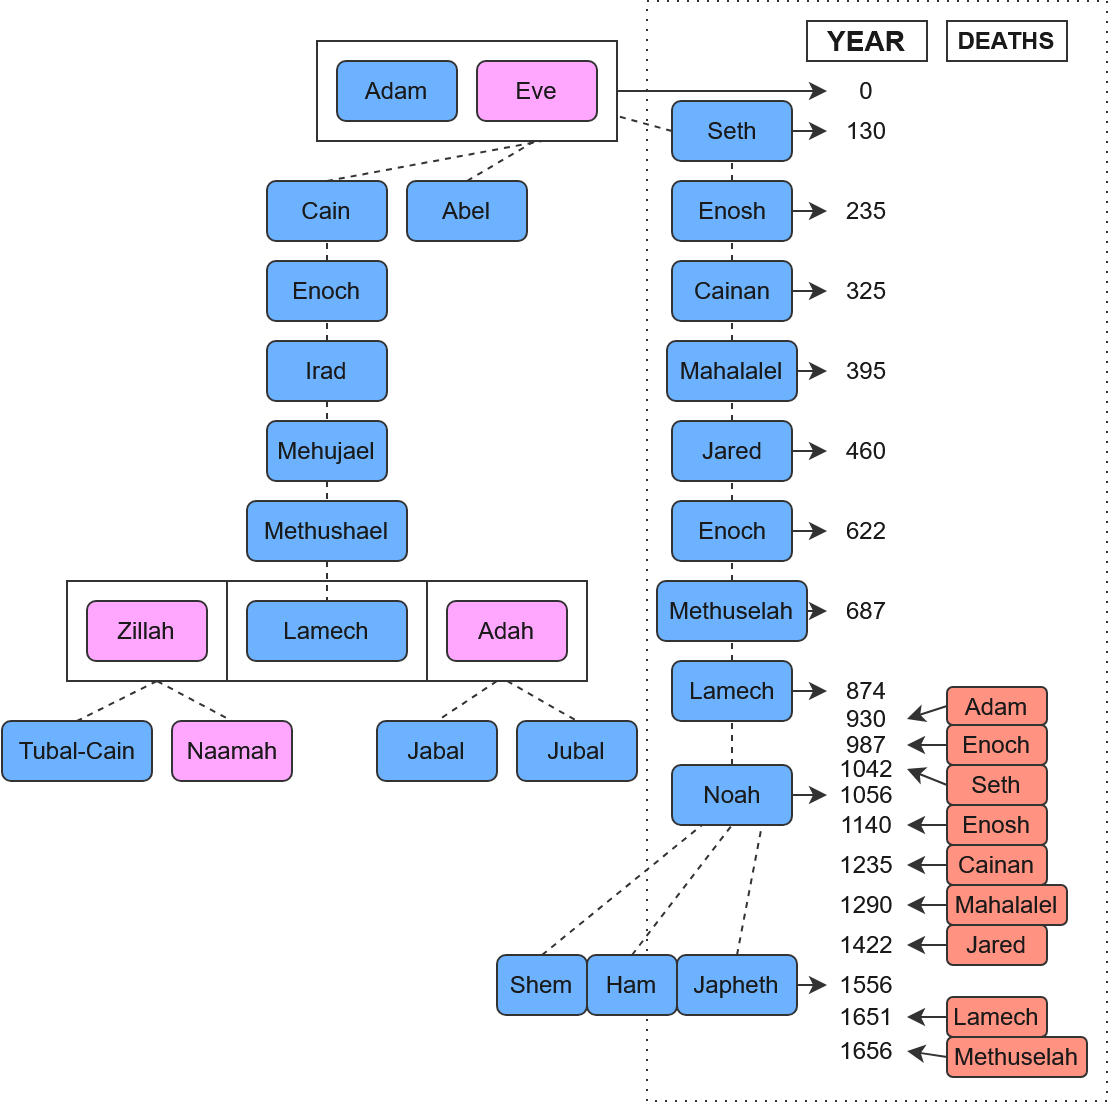
\includegraphics[width=\linewidth]{images/genealogies/noahs_genealogy.png}
  \caption{This is a diagram showing the genealogy of the family of Adam's as outlined in \bref{Genesis 4} and \bref{Genesis 5}. It ends with Noah's three children. Males are depicted in blue, while females are pink. Births are depicted as branching off from the mother. Marriages are depicted with a rectangular border around the couple. The genealogy between Seth and Noah have timeline markers showing the year of birth and death (death is shown for most, but not all). This diagram was created by me using the draw.io tool \cite{draw.io}.}
  \label{fig:noahs_genealogy}
\end{figure}
%% Chapter 6 of Genesis
\bookchapter{The Wickedness And Judgment\index{Judgment} of Man}


\bverse Now it came to pass, when men began to multiply on the face of the earth\index{Earth}, and daughters were born to them,
\bverse that the sons\vmark{a} of God saw the daughters of men, that they \textit{were} beautiful; and they took wives for themselves of all whom they chose.
	\translationnote{a}{The word `sons' here (Strong's 1121\cite{Strong's GodRules}) means children, people, grandsons, youth, etc. Since Adam\index{Adam} was directly created by God, any of his descendants could fall into this category. The `sons of God' distinction could be used to specifically refer to people who were following Gods and not those who strayed from his ways.}

\bverse And the \lord said, ``My Spirit shall not strive with man forever, for he \textit{is} indeed flesh; yet his days shall be one hundred and twenty years.''
\bverse There were giants\vmark{a} on the earth\index{Earth} in those days, and also afterward\vmark{b}, when the sons of God\vmark{c} came in to the daughters of men and they bore \textit{children} to them.
	\translationnote{a}{This term for `giant' (Strong's 5303\cite{Strong's GodRules}), is also known as `the Nephilim' has a bit of debate around it. Regardless, it means that there were a group of people with unusually large size and strength.}
	\contextnote{b}{This is likely referring to after the flood, since we also see giants mentioned after this time period in \bref{Numbers 13:33}.}
	\philosophicalnote{c}{Some argue that the `sons of God' here is angels (or demons), and thus the spirit beings created offspring with humans. The word for sons here does not really fit that at all (see the note on \bref{Genesis 6:2}).}

\bverse Those \textit{were} the mighty men who \textit{were} of old, men of renown.
\bverse 
\bverse 
\bverse 
\bverse 
\bverse 
\bverse 
\bverse 
\bverse 
\bverse 
\bverse 
\bverse 
\bverse 
\bverse 
\bverse 
\bverse 
\bverse 
\bverse 

%% Chapter 7 of Genesis
\bookchapter{The Great Flood}

\bverse 
\bverse 
\bverse 
\bverse 
\bverse 
\bverse 
\bverse 
\bverse 
\bverse 
\bverse 
\bverse 
\bverse 
\bverse 
\bverse 
\bverse 
\bverse 
\bverse 
\bverse 
\bverse 
\bverse 
\bverse 
\bverse 
\bverse 
\bverse 

%% Chapter 8 of Genesis
\bookchapter{Noah’s Deliverance}

\bverse Then God remembered Noah, and every living thing, and all the animals that \textit{were} with him in the ark. And God made a wind to pass over the earth, and the waters subsided.
\bverse The fountains of the deep\vmark{a} and the windows of heaven were also stopped, and the rain from heaven was restrained.
	\contextnote{a}{The `fountains of the deep' are clearly referred to here as something separate from the `rain from heaven,' which supports the idea that water was coming from within earth as well and not just from the rain. This is also referenced in \bref{Genesis 7:11}.}

\bverse And the waters receded continually from the earth\vmark{a}. At the end of the hundred and fifty days the waters decreased.
	\literarynote{a}{This is a literary technique that is used throughout these books (see \bref{Genesis 2:8}, \bref{Genesis 2:15}, and others). In \bref{Genesis 8:1}, it clearly states the waters subsided (implying completion). However, it follows up by saying the waters were receding continually - which may seem out of order and thus contradictory. This literary format is seen repeatedly and clearly expands on the statement made prior to this rather than giving specific accounts in order.}

\bverse Then the ark rested in the seventh month, the seventeenth day of the month, on the mountains of Ararat.
\bverse And the waters decreased continually until the tenth month. In the tenth \textit{month}, on the first \textit{day} of the month, the tops of the mountains were seen.
	\sciencenote{}{A question arises - does the earth have enough water to fit this flood account? A simple calculation based on a few key details suggests the answer is yes. First, the ocean water alone would not provide enough water to flood the earth in this manner. Thus, the ``fountains of the deep'' outlined in \bref{Genesis 8:2} and \bref{Genesis 7:11} are key to understanding how this is possible - which suggests water came from deep within earth, and not just from the oceans. To determine approximately how much water would be needed to flood the earth, the formula for the volume of a sphere can be used: $\frac{4}{3}\pi r^3$. Assuming earth is a perfect sphere and there are about as many hills and mountains as there are valleys and ravines (assuming terrain averages out to sea level, excluding oceans and filled basins), we can estimate the amount of water by finding the volume of that sphere from the highest mountain (Mount Everest at 6386.8 km from the center of the earth) to sea level (radius of earth which is about 6378.0 km from the center of the earth). This yields a total volume of water approximately three times that of Earth’s oceans\footnote{\begin{minipage}[t]{\linewidth}The results for these calculations were obtained from a Google featured snippet displaying the value directly in the search results after prompting Google with these questions. The calculations and conversions were done using Wolfram Alpha's computational engine \cite{WolframAlpha}. This calculation is ``$4*pi*(6384.8^3 - 6378.0^3)/3$ km$^3$'', which gave ``$\approx 3\times$ volume of Earth's oceans ($1.332\times10^9$ km$^3$)'' as an automatically generated comparison value. When entering in this calculation as miles instead of kilometers, the results was 3.4 times the volume of earths oceans (slightly more precise).\end{minipage}}. According to the Brookhaven National Laboratory, there is evidence for oceans of water deep in the earth. One fascinating statement on the subject (which should be more than enough to suggest this may be possible) is ``If just one percent of the weight of mantle rock located in the transition zone is \ce{H2O}, that would be equivalent to nearly three times the amount of water in our oceans, the researchers said'' \cite{deep earth water}. }
	\sermonnote{}{I wrote a sermonette on this topic  titled \textit{Fountains of The Deep}, which covers it a bit more concisely \cite{Antonius' Sermonettes}.}
	
\bverse So it came to pass, at the end of the forty days, that Noah opened the window of the ark which he had made.
\bverse Then he sent out a raven, which kept going to and fro until the waters had dried from the earth.
\bverse He also sent out from himself a dove, to see if the waters had receded from the face of the ground.
\bverse But the dove found no resting place for the sole of her foot, and she returned into the ark to him, for the waters \textit{were} on the face of the whole earth. So he put out his hand and took her, and drew her into the ark himself.
\bverse And he waited yet another seven days, and again he sent the dove out from the ark.
\bverse Then the dove came to him in the evening, and behold, a freshly plucked olive leaf\vmark{a} \textit{was} in her mouth; and Noah knew that the waters had receded from the earth.
	\questionnote{a}{This is interesting. Plants are obviously in a different category than the animals and people of the earth as they did not need saved by the ark. Perhaps this is part of what is meant by \textit{the breath of life} in \bref{Genesis 7:15} and \bref{Genesis 7:22}. However, how did an olive tree grow enough to bring forth olive leaves for the dove to pluck? It's possible it was just a freshly sprouted plant (small/tiny), and just a small sproutling (this can easily happen in a few days) and would likely be the case.}

\bverse So he waited yet another seven days and sent out a dove, which did not return again to him anymore. 
\bverse And it came to pass in the six hundred and first year, in the first \textit{month}, the first \textit{day} of the month\vmark{a}, that the waters were dried up from the earth; and Noah removed the covering of the ark and looked, and indeed the surface of the ground was dry.
	\contextnote{a}{This time is a reference to Noah's years on the earth. When the flood happened, he was 600 years old (see figure \ref{fig:noahs_genealogy} and \bref{Genesis 7:6}).}
	
\bverse And in the second month, on the twenty-seventh day of the month, the earth was dried.
\bverse Then God spoke to Noah, saying,
\bverse ``Go out of the ark, you and your wife, and your sons and your sons' wives with you.
\bverse Bring out with you every living thing of all flesh that \textit{is} with you: birds and cattle and every creeping thing that creeps on the earth, so that they may abound on the earth, and be fruitful and multiply on the earth.''
\bverse So Noah went out, and his sons and his wife and his sons' wives with him.
\bverse Every animal, every creeping thing, every bird, \textit{and} whatever creeps on the earth, according to their families, went out from the ark.

\bmarkerdown{God’s Covenant\index{Covenant} with Creation}

\bverse Then Noah built an altar to the \lord, and took of every clean animal and of every clean bird, and offered burnt offerings on the altar.
	\contextnote{}{This is the first time a \textit{burnt offering} is explicitly mentioned in scripture. It is possible that Abel's offering in \bref{Genesis 4:4}, though it does not state explicitly that it is a \text{burnt} offering. The laws around offerings have not yet been elaborated on or explained.}	

\bverse And the \lord smelled a smooth aroma. Then the \lord said in His heart, ``I will never again curse the ground for man's sake, although the imagination\vmark{a} of man's heart \textit{is} evil from his youth; nor will I again destroy every living thing as I have done.
	\translationnote{a}{The word `imagination' (Strong's 3336 \cite{Strong's GodRules}) means framing, or figuratively form. It can be thought of as \textit{intent} or \textit{thoughts} in this context.}

\begin{quotation}
\bverse ``While the earth remains, Seedtime and harvest, Cold and heat, Winter and summer, And day and night, Shall not cease.''
\end{quotation}

%% Chapter 9 of Genesis
\bookchapter{God's Promise to Noah\index{Noah}}

\bverse So God blessed Noah and his sons, and said to them: ``Be fruitful and multiply, and fill the earth.
\bverse And the fear of you and the dread of you shall be on every beast of the earth, on every bird of the air, on all that move \textit{on} the earth, and on all the fish of the sea. They are given into your hand.
\bverse Every moving thing that lives shall be food for you\vmark{a}. I have given you all things, even as the green herbs.
	\questionnote{a}{This scripture (as read) make it seem like anything/all living things on earth are good for food. He is speaking here to Noah and his sons. How does this reconcile with \bref{Deuteronomy 14} (the food laws)?}

\bverse But you shall not eat flesh with its life, \textit{that is}, its blood.
	\doctrinenote{}{This makes it clear that you are NOT to eat the blood of animals.}

\bverse Surely for your lifeblood I will demand \textit{a reckoning}; from the hand of every beast I will require it, and from the hand of man. From the hand of every man's brother I will require the life of man.
\begin{quotation}
\bverse Whoever sheds man's blood, By man his blood shall be shed; For in the image of God He made man. 
\bverse And as for you, be fruitful and multiply; Bring forth abundantly in the earth And multiply in it.''
\end{quotation}
\bverse Then God spoke to Noah and to his sons with him, saying:
\bverse ``And as for Me, behold, I establish My covenant with you and with your descendants after you,
\bverse and with every living creature that \textit{is} with you: the birds, the cattle, and every beast of the earth with you, of all that go our of the ark, every beast of the earth.
\bverse Thus I establish My covenant with you: Never again shall all flesh be cut off by the waters of the flood; never again shall there be a flood to destroy the earth.
\bverse And God said: ``This \textit{is} the sign of the covenant which I make between Me and you, and every living creature that \textit{is} with you, for perpetual generations:
\bverse I set My rainbow in the cloud, and it shall be for the sign of the covenant between Me and the earth.
\bverse It shall be, when I bring a cloud over the earth, that the rainbow shall be seen in the cloud;
\bverse and I will remember My covenant which \textit{is} between Me and you and every living creature of all flesh; the waters shall never again become a flood to destroy all flesh.
\bverse The rainbow shall be in the cloud, and I will look on it to remember the everlasting covenant between God and every living creature of all flesh that \textit{is} on the earth.''
\bverse And God said to Noah, ``This \textit{is} the sign of the covenant which I have established between Me and all flesh that is on the earth.''

\bmarkerdown{Noah and His Sons}

\bverse Now the sons of Noah who went out of the ark were Shem, Ham, and Japheth. And Ham \textit{was} the father of Canaan\vmark{a}.
	\translationnote{a}{The word/name for `Canaan' here (Strong's 3667 \cite{Strong's GodRules}) means `lowland'.}

\bverse These three \text{were} the sons of Noah, and from these the whole earth was populated.
\bverse And Noah began \textit{to be} a farmer, and he planted a vineyard.
\bverse Then he drank of the wine and was drunk, and became uncovered in his tent.
\bverse And Ham, the father of Canaan, saw the nakedness of his father, and told his two brothers outside.
\bverse But Shem and Japheth took a garment, laid \textit{it} on both their shoulders, and went backward and covered the nakedness of their father. Their faces \textit{were} turned away, and they did not see their father's nakedness.
\bverse So Noah awoke from his wine, and knew what his younger son had done to him.
\bverse Then he said:
\begin{quotation}
``Cursed \textit{be} Canaan; A servant of servants He shall be to his brethren.''
\end{quotation}
\bverse And he said:
\begin{quotation}
``Blessed \textit{be} the \lord, The God of Shem, And may Canaan be his servant.
\bverse May God enlarge Japheth, And may he dwell in the tents of Shem; And may Canaan be his servant.''
\end{quotation}

\bverse And Noah lived after the flood three hundred and fifty years.
\bverse So all the days of Noah were nine hundred and fifty years; and he died.
	\timelinenote{}{At the time of Noah's death, 2006 years have passed since the creation of Adam (see figure \ref{fig:noahs_genealogy}).}

%% Chapter 10 of Genesis
\bookchapter{Nations Descended from Noah}

\bverse Now this \textit{is} the genealogy of the sons of Noah: Shem, Ham, and Japheth. And sons were born to them after the flood.
\bverse The sons of Japheth \textit{were} Gomer, Magog, Madai, Javan, Tubal, Meshech, and Tiras.
\bverse The sons of Gomer \textit{were} Ashkenaz, Riphath, and Togarmah.
\bverse The sons of Javan \textit{were} Elishah, Tarshish, Kittim, and Dodanim.
\bverse From these the coastland \textit{peoples} of the Gentiles were separated into their lands, everyone according to his language, according to their families, into their nations.
\bverse The sons of Ham \textit{were} Cush, Mizraim, Put, and Canaan.
\bverse The sons of Cush \textit{were} Seba, Havilah, Sabtah, Raamah, and Sabtechah; and the sons of Raamah \textit{were} Sheba and Dedan.
\bverse 
\bverse 
\bverse 
\bverse 
\bverse 
\bverse 
\bverse 
\bverse 
\bverse 
\bverse 
\bverse 
\bverse 
\bverse 
\bverse 
\bverse 
\bverse 
\bverse 
\bverse 
\bverse 
\bverse 
\bverse 
\bverse 
\bverse 
\bverse 
\bverse 

%% Chapter 11 of Genesis
\bookchapter{The Tower of Babel}

\bverse Now the whole earth had one language\vmark{a} and one speech.
	\translationnote{a}{The word for `language' here (Strong's 8193 \cite{Strong's GodRules}) is distinct from the word `tongues' used in \bref{Genesis 10}. This word more literally means \textit{language} or \textit{speech}.}
	\contextnote{a}{In \bref{Genesis 10}, it makes it seem like the different lineages were separated based on their \textit{tongues}, which could mean languages. However, to be under one language here means either that \textit{tongues} specifically refers to different dialects \textit{or} that this languages is referring to something else such as the language of mathematics. We see in modern society that even though many countries have different languages, we all can write in common terms using something like mathematics. Though the `one speech' makes it seem like a more literal form of spoken language.}

\bverse And it came to pass, as they journeyed from the east, that they found a plain in the land of Shinar, and they dwelt there.
\bverse Then they said to one another, ``Come, let us make bricks and bake \textit{them} thoroughly.'' They had brick for stone, and they had asphalt for mortar.
\bverse And they said, ``Come, let us build ourselves a city, and a tower whos top \is in the heavens; let us make a name for ourselves, lest we be scattered abroad over the face of the whole earth.''
	\questionnote{}{We see here that they (the people of the time) did \textit{not} want to be scattered abroad over the face of the earth. Perhaps they knew something about sticking together that would give them an advantage? I wonder why they did not want to spread out. Perhaps they were advancing too quickly?}

\bverse But the \lord came down to see the city and the tower which the sons of men had build.
\bverse And the \lord said, ``Indeed the people \are one and they all have one language, and this is what they begin to do; now nothing that they propose to do will be withheld from them.
\bverse Come, let Us go down and there confuse their language, that they may not understand one another's speech.''
\bverse So the \lord scattered them abroad from there over the face of all the earth, and they ceased building the city.
\bverse Therefore its name is called Babel, because there the \lord confused the language of all the earth; and from there the \lord scattered them abroad over the face of all the earth.
	\questionnote{}{For some reason, the \lord decided that he had to scatter them abroad the face of the earth - which is directly opposed to what the people wanted (see \bref{Genesis 11:4}). Why did he find the need or desire to do this?}

\bmarkerdown{\name{Shem}'s Descendants}

\bverse This \is the genealogy of \name{Shem}: \name{Shem} was one hundred years old, and begot \name{Arphaxad} two years after the flood.
\bverse After he begot \name{Arphaxad}, \name{Shem} lived five hundred years, and begot sons and daughters.
\bverse \name{Arphaxad} lived thirty-five years, and begot \name{Salah}.
\bverse After he begot \name{Salah}, \name{Arphaxad} lived four hundred and three years, and begot sons and daughters.
\bverse \name{Salah} lived thirty years, and begot \name{Eber}.
\bverse After he begot \name{Eber}, \name{Salah} lived four hundred and three years, and begot sons and daughters.
\bverse \name{Eber} lived thirty-four years, and begot \name{Peleg}.
\bverse After he begot \name{Peleg}, \name{Eber} lived four hundred and thirty years, and begot sons and daughters.
\bverse \name{Peleg} lived thirty years, and begot \name{Reu}. 
\bverse After he begot \name{Reu}, \name{Peleg} lived two hundred and nine years, and begot sons and daughters.
\bverse \name{Reu} lived thirty-two years, and begot \name{Serug}.
\bverse After he begot \name{Serug}, \name{Reu} lived two hundred and seven years, and begot sons and daughters.
\bverse \name{Serug} lived thirty years, and begot \name{Nahor}.
\bverse After he begot \name{Nahor}, \name{Serug} lived two hundred years, and begot sons and daughters.
\bverse \name{Nahor} lived twenty-nine years, and begot \name{Terah}.
\bverse After he begot \name{Terah}, \name{Nahor} lived one hundred and nineteen years, and begot sons and daughters.
\bverse Now \name{Terah} lived seventy years, and begot \name{Abram}, \name{Nahor}, and \name{Haran}.



\begin{figure}[h] % h=here
	\centering
	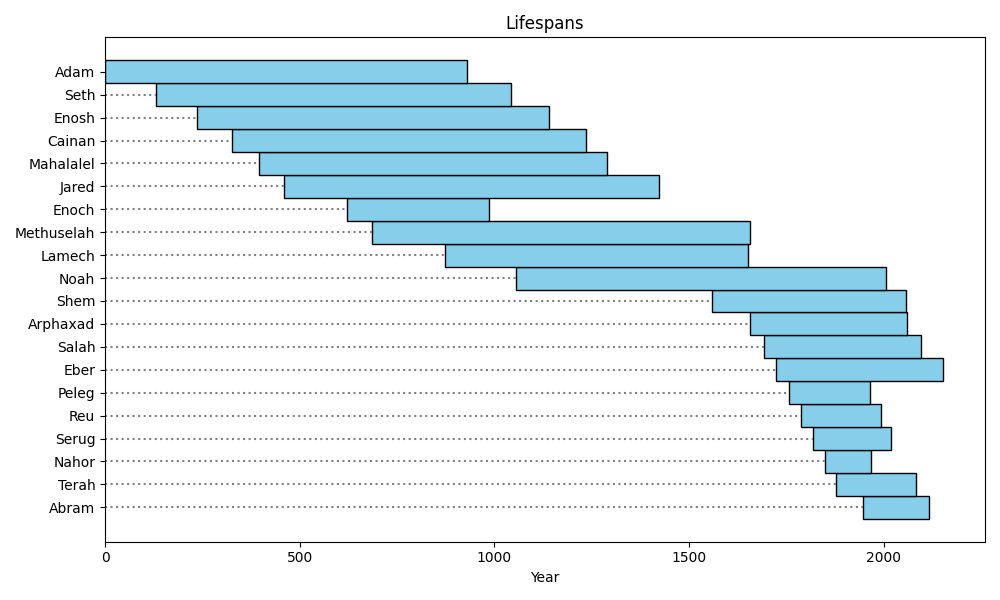
\includegraphics[width=0.95\linewidth]{images/lifespans/pre_abram_lifespans.png}
	\caption{This chart shows the lifespans of various individuals whose total lifespans are mentioned. The chart covers individuals up to and including \name{Abram}.}
	\label{fig:pre_adam_lifespans}
\end{figure}



\bmarkerdown{\name{Terah}'s Descendants}

\bverse This is the genealogy of \name{Terah}: \name{Terah} begot \name{Abram}, \name{Nahor}, and \name{Haran}. \name{Haran} begot \name{Lot}.
\bverse And \name{Haran} died before his father \name{Terah} in his native land, in Ur of the Chaldeans.
\bverse Then \name{Abram} and \name{Nahor} took wives: the name of \name{Abram}'s wife \was \name{Sarai}, and the name of \name{Nahor}'s wife, \name{Milcah}, the daughter of \name{Haran} the father of \name{Milcah} and the father of \name{Iscah}.
\bverse But \name{Sarai} was barren; she had no child.
\bverse And \name{Terah} took his son \name{Abram} and his grandson \name{Lot}, the son of \name{Haran}, and his daughter-in-law \name{Sarai}, his son \name{Abram}'s wife, and they went out with them from Ur of the Chaldeans to go to the land of Canaan; and they came to Haran and dwelt there.
\bverse So the days of \name{Terah} were two hundred and five years, and \name{Terah} died in Haran.



\begin{figure}[htbp] % h=here, t=top, b=bottom, p=page
	\centering
	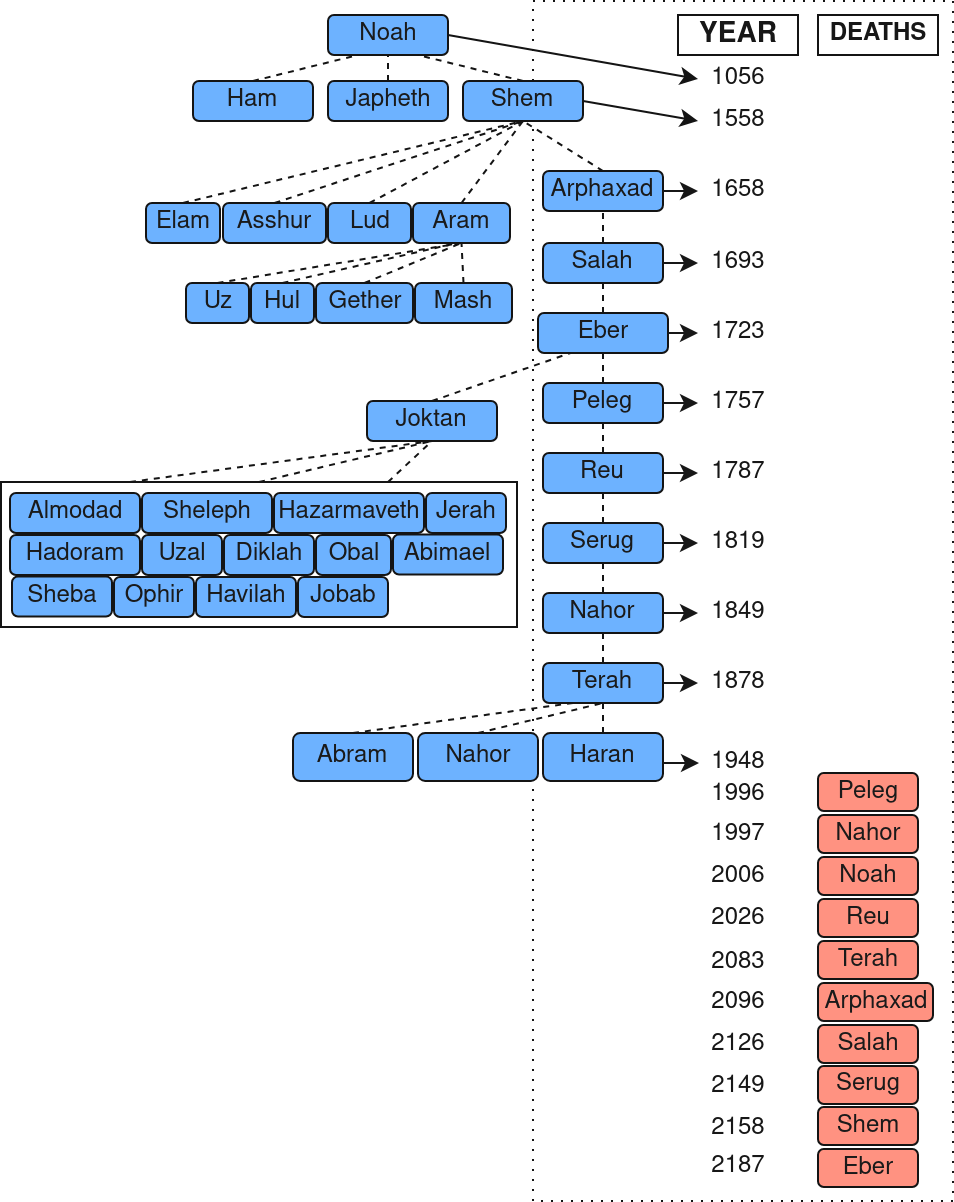
\includegraphics[width=0.9\linewidth]{images/genealogies/shems_genealogy.png}
	\caption{This is a diagram showing the genealogy of the family of \name{Shem} as outlined in \bref{Genesis 10} and \bref{Genesis 11}. It ends with \name{Terah}'s three children (\name{Abram}, \name{Nahor}, and \name{Haran}) from \bref{Genesis 11:26}. Males are depicted in blue. The genealogy shows timeline markers showing the year of birth and death for many of the descendants (where outlined in \bref{Genesis 11}), which are primarily in the dotted box. The box with a bold border represents all the sons of \name{Joktan}. This diagram was created by me using the draw.io tool \cite{draw.io}.}
	\label{fig:shems_genealogy}
\end{figure}

%% Chapter 12 of Genesis
\bookchapter{Promises to \name{Abram}}

\bverse Now the \lord had said to \name{Abram}:
\begin{bquotation}
``Get out of your country, From your family And from your father's house, To a land that I will show you. \bverse I will make you a great nation; I will bless you And make your name great; And you shall be a blessing. \bverse I will bless those who bless you, And I will curse him who curses you; And in you all the families of the earth shall be blessed.''
\end{bquotation}

\bverse So \name{Abram} departed as the \lord had spoken to him, and \name{Lot} went with him. And \name{Abram} \was seventy-five years old when he departed from Haran.
\bverse Then \name{Abram} took \name{Sarai} his wife and \name{Lot} his brother's son, and all their possessions that they had gathered, and the people whom they had acquired in Haran, and they departed to go to the land of Canaan. So they came to the land of Canaan.
\bverse \name{Abram} passed through the land to the place of Shechem, as far as the terebinth tree of Moreh. And the Canaanites \were then in the land.
\bverse Then the \lord appeared to \name{Abram} and said, ``To your descendants I will give this land.'' And there he build an altar to the \lord, who had appeared to him.
\bverse And he moved from there to the mountain east of Bethel, and he pitched his tent \textit{with} Bethel on the west and Ai on the east; there he built an altar to the \lord and called on the name of the \lord.
\bverse So \name{Abram} journeyed, going on still toward the South.

\bmarker{Abram in Egypt}

\bverse Now there was a famine in the land, and \name{Abram} went down to Egypt to dwell there, for the famine \was severe in the land.
\bverse And it came to pass, when he was close to entering Egypt, that he said to \name{Sarai} his wife, ``Indeed I know that you \are a woman of beautiful countenance.
\bverse Therefore it will happen, when the Egyptians see you, that they will say, `This \is his wife'; and they will kill me, but they will let you live.
\bverse Please say you \are my sister, that it may be well with me for your sake, and that I may live because of you.''
\bverse So it was, when \name{Abram} came into Egypt, that the Egyptians saw the woman, that she \was very beautiful.
\bverse The princes of Pharaoh also saw her and commended her to Pharaoh. And the women was taken to Pharaoh's house.
\bverse He treated \name{Abram} well for her sake. He had sheep, oxen, male donkeys, male and female servants, female donkeys, and camels.
	\questionnote{}{Why are male and female donkey's separated here in this list? What is the significance - perhaps something culturally significant?}

\bverse But the \lord plagued Pharaoh and his house with great plagues because of \name{Sarai}, \name{Abram}'s wife.
\bverse And Pharaoh called \name{Abram} and said ``What \is this you have done to me? Why did you say `She \is my sister'? I might have taken her as my wife. Now therefore, here is your wife; take \textit{her} and go your way.''
\bverse So Pharaoh commanded \textit{his} men concerning him; and they sent him away with his wife and all that he had.
%% Chapter 13 of Genesis
\bookchapter{}

%% Chapter 14 of Genesis
\bookchapter{\name{Lot}'s Captivity and Rescue}

\bverse And it came to pass in the days of \name{Amraphel} king of Shinar, \name{Arioch} king of Ellasar, \name{Chedorlaomer} king of Elam, and \name{Tidal} king of nations,
\bverse 
\bverse 
\bverse 
\bverse 
\bverse 
\bverse 
\bverse 
\bverse 
\bverse 
\bverse 
\bverse 
\bverse 
\bverse 
\bverse 
\bverse 
\bverse 
\bverse 
\bverse 
\bverse 
\bverse 
\bverse 
\bverse 
\bverse 

%% Chapter 15 of Genesis
\bookchapter{God's Covenant with \name{Abram}}

\bverse After these things the word of the \lord came to \name{Abram} in a vision, saying, ``Do not be afraid, \name{Abram}. I \textit{am} your shield, your exceedingly great reward.''
\bverse But \name{Abram} said, ``Lord \god\unskip\vmark{a}, what will You give me, seeing I go childless, and the heir of my house \is \name{Eliezer} of \location{Damascus}?''
	\translationnote{a}{This is a somewhat different representation of the translation. Instead of the usual `\lord' used for God's proper name, the `Lord' here is the Hebrew word `Adonay' (Strong's 136 \cite{Hebrew Concordance}) which literally means \textit{lord} or \textit{master}, whereas the `\god' is God's proper name, which usually appears as `\lord'. So another way to write this could be `lord \lord', but that is a little weird in English.}

\bverse But \name{Abram} said, ``Look, You have given me no offspring; indeed one born in my house is my heir!''
\bverse And behold, the word of the \lord \textit{came} to him, saying, ``This one shall not be your heir, but one who will come from your own body shall be your heir.'' 
\bverse Then He brought him outside and said, ``Look, now toward heaven, and count the stars if you are able to number them.'' And He said to him, ``So shall your descendants be.''
\bverse And he believed in the \lord, and He accounted it to him for righteousness.
\bverse Then He said to him, ``I \textit{am} the \lord, who brought you out of \location{Ur} of the \people{Chaldeans}, to give you this land to inherit it.''
\bverse And he said, ``Lord \god, how shall I know that I will inherit it?''
\bverse So He said to him, ``Bring Me a three-year-old heifer, a three-year-old female goat, a three-year-old ram, a turtledove, and a young pigeon.''
\bverse Then he brought all these to Him and cut them in two, down the middle, and placed each piece opposite the other; but he did not cut the birds in two.
	\questionnote{}{Is there some sort of symbolism here with cutting the animals in half and then \textit{not} cutting the birds?}

\bverse And when the vultures came down on the carcasses, \name{Abram} drove them away.
\bverse Now when the sun was going down, a deep sleep fell upon \name{Abram}; and behold, horror \textit{and} great darkness fell upon him. 
\bverse Then He said to \name{Abram}: ``Know certainly that your descendants will be strangers in a land \textit{that is} not theirs, and will serve them, and they will afflict them four hundred years.
	\contextnote{}{This is referring to the slavery in \location{Egypt}, where his descendants will be slaves and eventually freed after 400 years.}

\bverse And also the nation whom they serve I will judge; afterward they shall come out with great possessions.
\bverse Now as for you, you shall go to your fathers in peace; you shall be buried at a good old age.
\bverse But in the fourth generation they shall return here, for the iniquity of the \people{Amorites} \textit{is} not yet complete.''
\bverse And it came to pass, when the sun went down and it was dark, that behold, there appeared a smoking oven and a burning torch that passed between those pieces.
\bverse On the same day the \lord made a covenant with \name{Abram}, saying:
\bverse ``To your descendants I have given this land, from the river of \location{Egypt} to the great river, the \location{River of Euphrates}--
\bverse the \people{Kenites}, the \people{Kenezzites}, the \people{Kadmonites},
\bverse the \people{Hittites}, the \people{Perizzites}, the \people{Raphaim}, the \people{Amorites}, the \people{Canaanites}, the \people{Girgashites}, and the \people{Jebusites}.''

%% Chapter 16 of Genesis
\bookchapter{}

%% Chapter 17 of Genesis
\bookchapter{}

\bverse{}
\bverse{}
\bverse{}
\bverse{}
\bverse{}
\bverse{}
\bverse{}
\bverse{}
\bverse{}
\bverse{}
\bverse{}
\bverse{}
\bverse{}
\bverse{}
\bverse{}
\bverse{}
\bverse{}
\bverse{}
\bverse{}
\bverse{}
\bverse{}
\bverse{}
\bverse{}
\bverse{}
\bverse{}
\bverse{}
\bverse{}

%% Chapter 18 of Genesis
\bookchapter{}

%% Chapter 19 of Genesis
\bookchapter{\location{Sodom}'s Depravity}

\bverse 
\bverse 
\bverse 
\bverse 
\bverse 
\bverse 
\bverse 
\bverse 
\bverse 
\bverse 
\bverse 
\bverse 
\bverse 
\bverse 
\bverse 
\bverse 
\bverse 
\bverse 
\bverse 
\bverse 
\bverse 
\bverse 
\bverse 
\bverse 
\bverse 
\bverse 
\bverse 
\bverse 
\bverse 
\bverse 
\bverse 
\bverse 
\bverse 
\bverse 
\bverse 
\bverse 
\bverse 
\bverse 

%% Chapter 20 of Genesis
\bookchapter{}

%% Chapter 21 of Genesis
\bookchapter{}

\bverse 
\bverse 
\bverse 
\bverse 
\bverse 
\bverse 
\bverse 
\bverse 
\bverse 
\bverse 
\bverse 
\bverse 
\bverse 
\bverse 
\bverse 
\bverse 
\bverse 
\bverse 
\bverse 
\bverse 
\bverse 
\bverse 
\bverse 
\bverse 
\bverse 
\bverse 
\bverse 
\bverse 
\bverse 
\bverse 
\bverse 
\bverse 
\bverse 
\bverse 

%% Chapter 22 of Genesis
\bookchapter{}

\bverse{}
\bverse{}
\bverse{}
\bverse{}
\bverse{}
\bverse{}
\bverse{}
\bverse{}
\bverse{}
\bverse{}
\bverse{}
\bverse{}
\bverse{}
\bverse{}
\bverse{}
\bverse{}
\bverse{}
\bverse{}
\bverse{}
\bverse{}
\bverse{}
\bverse{}
\bverse{}
\bverse{}

%% Chapter 23 of Genesis
\bookchapter{}

\bverse{}
\bverse{}
\bverse{}
\bverse{}
\bverse{}
\bverse{}
\bverse{}
\bverse{}
\bverse{}
\bverse{}
\bverse{}
\bverse{}
\bverse{}
\bverse{}
\bverse{}
\bverse{}
\bverse{}
\bverse{}
\bverse{}
\bverse{}

%% Chapter 24 of Genesis
\bookchapter{}

%% Chapter 25 of Genesis
\bookchapter{}

\bverse{}
\bverse{}
\bverse{}
\bverse{}
\bverse{}
\bverse{}
\bverse{}
\bverse{}
\bverse{}
\bverse{}
\bverse{}
\bverse{}
\bverse{}
\bverse{}
\bverse{}
\bverse{}
\bverse{}
\bverse{}
\bverse{}
\bverse{}
\bverse{}
\bverse{}
\bverse{}
\bverse{}
\bverse{}
\bverse{}
\bverse{}
\bverse{}
\bverse{}
\bverse{}
\bverse{}
\bverse{}
\bverse{}
\bverse{}

%% Chapter 26 of Genesis
\bookchapter{}

%% Chapter 27 of Genesis
\bookchapter{}

\bverse{}
\bverse{}
\bverse{}
\bverse{}
\bverse{}
\bverse{}
\bverse{}
\bverse{}
\bverse{}
\bverse{}
\bverse{}
\bverse{}
\bverse{}
\bverse{}
\bverse{}
\bverse{}
\bverse{}
\bverse{}
\bverse{}
\bverse{}
\bverse{}
\bverse{}
\bverse{}
\bverse{}
\bverse{}
\bverse{}
\bverse{}
\bverse{}
\bverse{}
\bverse{}
\bverse{}
\bverse{}
\bverse{}
\bverse{}
\bverse{}
\bverse{}
\bverse{}
\bverse{}
\bverse{}
\bverse{}
\bverse{}
\bverse{}
\bverse{}
\bverse{}
\bverse{}
\bverse{}

%% Chapter 28 of Genesis
\bookchapter{}

\bverse 
\bverse 
\bverse 
\bverse 
\bverse 
\bverse 
\bverse 
\bverse 
\bverse 
\bverse 
\bverse 
\bverse 
\bverse 
\bverse 
\bverse 
\bverse 
\bverse 
\bverse 
\bverse 
\bverse 
\bverse 
\bverse 

%% Chapter 29 of Genesis
\bookchapter{}

\bverse{}
\bverse{}
\bverse{}
\bverse{}
\bverse{}
\bverse{}
\bverse{}
\bverse{}
\bverse{}
\bverse{}
\bverse{}
\bverse{}
\bverse{}
\bverse{}
\bverse{}
\bverse{}
\bverse{}
\bverse{}
\bverse{}
\bverse{}
\bverse{}
\bverse{}
\bverse{}
\bverse{}
\bverse{}
\bverse{}
\bverse{}
\bverse{}
\bverse{}
\bverse{}
\bverse{}
\bverse{}
\bverse{}
\bverse{}
\bverse{}

%% Chapter 30 of Genesis
\bookchapter{}

\bverse 
\bverse 
\bverse 
\bverse 
\bverse 
\bverse 
\bverse 
\bverse 
\bverse 
\bverse 
\bverse 
\bverse 
\bverse 
\bverse 
\bverse 
\bverse 
\bverse 
\bverse 
\bverse 
\bverse 
\bverse 
\bverse 
\bverse 
\bverse 
\bverse 
\bverse 
\bverse 
\bverse 
\bverse 
\bverse 
\bverse 
\bverse 
\bverse 
\bverse 
\bverse 
\bverse 
\bverse 
\bverse 
\bverse 
\bverse 
\bverse 
\bverse 
\bverse 

%% Chapter 31 of Genesis
\bookchapter{}

\bverse 
\bverse 
\bverse 
\bverse 
\bverse 
\bverse 
\bverse 
\bverse 
\bverse 
\bverse 
\bverse 
\bverse 
\bverse 
\bverse 
\bverse 
\bverse 
\bverse 
\bverse 
\bverse 
\bverse 
\bverse 
\bverse 
\bverse 
\bverse 
\bverse 
\bverse 
\bverse 
\bverse 
\bverse 
\bverse 
\bverse 
\bverse 
\bverse 
\bverse 
\bverse 
\bverse 
\bverse 
\bverse 
\bverse 
\bverse 
\bverse 
\bverse 
\bverse 
\bverse 
\bverse 
\bverse 
\bverse 
\bverse 
\bverse 
\bverse 
\bverse 
\bverse 
\bverse 
\bverse 
\bverse 

%% Chapter 32 of Genesis
\bookchapter{}

\bverse 
\bverse 
\bverse 
\bverse 
\bverse 
\bverse 
\bverse 
\bverse 
\bverse 
\bverse 
\bverse 
\bverse 
\bverse 
\bverse 
\bverse 
\bverse 
\bverse 
\bverse 
\bverse 
\bverse 
\bverse 
\bverse 
\bverse 
\bverse 
\bverse 
\bverse 
\bverse 
\bverse 
\bverse 
\bverse 
\bverse 
\bverse 

%% Chapter 33 of Genesis
\bookchapter{}

\bverse{}
\bverse{}
\bverse{}
\bverse{}
\bverse{}
\bverse{}
\bverse{}
\bverse{}
\bverse{}
\bverse{}
\bverse{}
\bverse{}
\bverse{}
\bverse{}
\bverse{}
\bverse{}
\bverse{}
\bverse{}
\bverse{}
\bverse{}

%% Chapter 34 of Genesis
\bookchapter{}

\bverse{}
\bverse{}
\bverse{}
\bverse{}
\bverse{}
\bverse{}
\bverse{}
\bverse{}
\bverse{}
\bverse{}
\bverse{}
\bverse{}
\bverse{}
\bverse{}
\bverse{}
\bverse{}
\bverse{}
\bverse{}
\bverse{}
\bverse{}
\bverse{}
\bverse{}
\bverse{}
\bverse{}
\bverse{}
\bverse{}
\bverse{}
\bverse{}
\bverse{}
\bverse{}
\bverse{}

%% Chapter 35 of Genesis
\bookchapter{}

\bverse 
\bverse 
\bverse 
\bverse 
\bverse 
\bverse 
\bverse 
\bverse 
\bverse 
\bverse 
\bverse 
\bverse 
\bverse 
\bverse 
\bverse 
\bverse 
\bverse 
\bverse 
\bverse 
\bverse 
\bverse 
\bverse 
\bverse 
\bverse 
\bverse 
\bverse 
\bverse 
\bverse 
\bverse 

%% Chapter 36 of Genesis
\bookchapter{}

\bverse 
\bverse 
\bverse 
\bverse 
\bverse 
\bverse 
\bverse 
\bverse 
\bverse 
\bverse 
\bverse 
\bverse 
\bverse 
\bverse 
\bverse 
\bverse 
\bverse 
\bverse 
\bverse 
\bverse 
\bverse 
\bverse 
\bverse 
\bverse 
\bverse 
\bverse 
\bverse 
\bverse 
\bverse 
\bverse 
\bverse 
\bverse 
\bverse 
\bverse 
\bverse 
\bverse 
\bverse 
\bverse 
\bverse 
\bverse 
\bverse 
\bverse 
\bverse 

%% Chapter 37 of Genesis
\bookchapter{}

\bverse 
\bverse 
\bverse 
\bverse 
\bverse 
\bverse 
\bverse 
\bverse 
\bverse 
\bverse 
\bverse 
\bverse 
\bverse 
\bverse 
\bverse 
\bverse 
\bverse 
\bverse 
\bverse 
\bverse 
\bverse 
\bverse 
\bverse 
\bverse 
\bverse 
\bverse 
\bverse 
\bverse 
\bverse 
\bverse 
\bverse 
\bverse 
\bverse 
\bverse 
\bverse 
\bverse 

%% Chapter 38 of Genesis
\bookchapter{}

\bverse 
\bverse 
\bverse 
\bverse 
\bverse 
\bverse 
\bverse 
\bverse 
\bverse 
\bverse 
\bverse 
\bverse 
\bverse 
\bverse 
\bverse 
\bverse 
\bverse 
\bverse 
\bverse 
\bverse 
\bverse 
\bverse 
\bverse 
\bverse 
\bverse 
\bverse 
\bverse 
\bverse 
\bverse 
\bverse 

%% Chapter 39 of Genesis
\bookchapter{}

\bverse{}
\bverse{}
\bverse{}
\bverse{}
\bverse{}
\bverse{}
\bverse{}
\bverse{}
\bverse{}
\bverse{}
\bverse{}
\bverse{}
\bverse{}
\bverse{}
\bverse{}
\bverse{}
\bverse{}
\bverse{}
\bverse{}
\bverse{}
\bverse{}
\bverse{}
\bverse{}

%% Chapter 40 of Genesis
\bookchapter{}

%% Chapter 41 of Genesis
\bookchapter{}

\bverse{}
\bverse{}
\bverse{}
\bverse{}
\bverse{}
\bverse{}
\bverse{}
\bverse{}
\bverse{}
\bverse{}
\bverse{}
\bverse{}
\bverse{}
\bverse{}
\bverse{}
\bverse{}
\bverse{}
\bverse{}
\bverse{}
\bverse{}
\bverse{}
\bverse{}
\bverse{}
\bverse{}
\bverse{}
\bverse{}
\bverse{}
\bverse{}
\bverse{}
\bverse{}
\bverse{}
\bverse{}
\bverse{}
\bverse{}
\bverse{}
\bverse{}
\bverse{}
\bverse{}
\bverse{}
\bverse{}
\bverse{}
\bverse{}
\bverse{}
\bverse{}
\bverse{}
\bverse{}
\bverse{}
\bverse{}
\bverse{}
\bverse{}
\bverse{}
\bverse{}
\bverse{}
\bverse{}
\bverse{}
\bverse{}
\bverse{}

%% Chapter 42 of Genesis
\bookchapter{}

\bverse{}
\bverse{}
\bverse{}
\bverse{}
\bverse{}
\bverse{}
\bverse{}
\bverse{}
\bverse{}
\bverse{}
\bverse{}
\bverse{}
\bverse{}
\bverse{}
\bverse{}
\bverse{}
\bverse{}
\bverse{}
\bverse{}
\bverse{}
\bverse{}
\bverse{}
\bverse{}
\bverse{}
\bverse{}
\bverse{}
\bverse{}
\bverse{}
\bverse{}
\bverse{}
\bverse{}
\bverse{}
\bverse{}
\bverse{}
\bverse{}
\bverse{}
\bverse{}
\bverse{}

%% Chapter 43 of Genesis
\bookchapter{}

\bverse 
\bverse 
\bverse 
\bverse 
\bverse 
\bverse 
\bverse 
\bverse 
\bverse 
\bverse 
\bverse 
\bverse 
\bverse 
\bverse 
\bverse 
\bverse 
\bverse 
\bverse 
\bverse 
\bverse 
\bverse 
\bverse 
\bverse 
\bverse 
\bverse 
\bverse 
\bverse 
\bverse 
\bverse 
\bverse 
\bverse 
\bverse 
\bverse 
\bverse 

%% Chapter 44 of Genesis
\bookchapter{}

\bverse 
\bverse 
\bverse 
\bverse 
\bverse 
\bverse 
\bverse 
\bverse 
\bverse 
\bverse 
\bverse 
\bverse 
\bverse 
\bverse 
\bverse 
\bverse 
\bverse 
\bverse 
\bverse 
\bverse 
\bverse 
\bverse 
\bverse 
\bverse 
\bverse 
\bverse 
\bverse 
\bverse 
\bverse 
\bverse 
\bverse 
\bverse 
\bverse 
\bverse 

%% Chapter 45 of Genesis
\bookchapter{}

\bverse 
\bverse 
\bverse 
\bverse 
\bverse 
\bverse 
\bverse 
\bverse 
\bverse 
\bverse 
\bverse 
\bverse 
\bverse 
\bverse 
\bverse 
\bverse 
\bverse 
\bverse 
\bverse 
\bverse 
\bverse 
\bverse 
\bverse 
\bverse 
\bverse 
\bverse 
\bverse 
\bverse 

%% Chapter 46 of Genesis
\bookchapter{}

\bverse{}
\bverse{}
\bverse{}
\bverse{}
\bverse{}
\bverse{}
\bverse{}
\bverse{}
\bverse{}
\bverse{}
\bverse{}
\bverse{}
\bverse{}
\bverse{}
\bverse{}
\bverse{}
\bverse{}
\bverse{}
\bverse{}
\bverse{}
\bverse{}
\bverse{}
\bverse{}
\bverse{}
\bverse{}
\bverse{}
\bverse{}
\bverse{}
\bverse{}
\bverse{}
\bverse{}
\bverse{}
\bverse{}
\bverse{}

%% Chapter 47 of Genesis
\bookchapter{}

\bverse 
\bverse 
\bverse 
\bverse 
\bverse 
\bverse 
\bverse 
\bverse 
\bverse 
\bverse 
\bverse 
\bverse 
\bverse 
\bverse 
\bverse 
\bverse 
\bverse 
\bverse 
\bverse 
\bverse 
\bverse 
\bverse 
\bverse 
\bverse 
\bverse 
\bverse 
\bverse 
\bverse 
\bverse 
\bverse 
\bverse 

%% Chapter 48 of Genesis
\bookchapter{}

\bverse 
\bverse 
\bverse 
\bverse 
\bverse 
\bverse 
\bverse 
\bverse 
\bverse 
\bverse 
\bverse 
\bverse 
\bverse 
\bverse 
\bverse 
\bverse 
\bverse 
\bverse 
\bverse 
\bverse 
\bverse 
\bverse 

%% Chapter 49 of Genesis
\bookchapter{}

\bverse 
\bverse 
\bverse 
\bverse 
\bverse 
\bverse 
\bverse 
\bverse 
\bverse 
\bverse 
\bverse 
\bverse 
\bverse 
\bverse 
\bverse 
\bverse 
\bverse 
\bverse 
\bverse 
\bverse 
\bverse 
\bverse 
\bverse 
\bverse 
\bverse 
\bverse 
\bverse 
\bverse 
\bverse 
\bverse 
\bverse 
\bverse 
\bverse 

%% Chapter 50 of Genesis
\bookchapter{}


%\booktitle{Exodus}{}
%% Chapter 1 of Exodus
\bookchapter{}

\bverse{}
\bverse{}
\bverse{}
\bverse{}
\bverse{}
\bverse{}
\bverse{}
\bverse{}
\bverse{}
\bverse{}
\bverse{}
\bverse{}
\bverse{}
\bverse{}
\bverse{}
\bverse{}
\bverse{}
\bverse{}
\bverse{}
\bverse{}
\bverse{}
\bverse{}

%% Chapter 2 of Exodus
\bookchapter{}

\bverse{}
\bverse{}
\bverse{}
\bverse{}
\bverse{}
\bverse{}
\bverse{}
\bverse{}
\bverse{}
\bverse{}
\bverse{}
\bverse{}
\bverse{}
\bverse{}
\bverse{}
\bverse{}
\bverse{}
\bverse{}
\bverse{}
\bverse{}
\bverse{}
\bverse{}
\bverse{}
\bverse{}
\bverse{}

%% Chapter 3 of Exodus
\bookchapter{}

%% Chapter 4 of Exodus
\bookchapter{}

\bverse{}
\bverse{}
\bverse{}
\bverse{}
\bverse{}
\bverse{}
\bverse{}
\bverse{}
\bverse{}
\bverse{}
\bverse{}
\bverse{}
\bverse{}
\bverse{}
\bverse{}
\bverse{}
\bverse{}
\bverse{}
\bverse{}
\bverse{}
\bverse{}
\bverse{}
\bverse{}
\bverse{}
\bverse{}
\bverse{}
\bverse{}
\bverse{}
\bverse{}
\bverse{}
\bverse{}

%% Chapter 5 of Exodus
\bookchapter{}

\bverse{}
\bverse{}
\bverse{}
\bverse{}
\bverse{}
\bverse{}
\bverse{}
\bverse{}
\bverse{}
\bverse{}
\bverse{}
\bverse{}
\bverse{}
\bverse{}
\bverse{}
\bverse{}
\bverse{}
\bverse{}
\bverse{}
\bverse{}
\bverse{}
\bverse{}
\bverse{}

%% Chapter 6 of Exodus
\bookchapter{}

\bverse{}
\bverse{}
\bverse{}
\bverse{}
\bverse{}
\bverse{}
\bverse{}
\bverse{}
\bverse{}
\bverse{}
\bverse{}
\bverse{}
\bverse{}
\bverse{}
\bverse{}
\bverse{}
\bverse{}
\bverse{}
\bverse{}
\bverse{}
\bverse{}
\bverse{}
\bverse{}
\bverse{}
\bverse{}
\bverse{}
\bverse{}
\bverse{}
\bverse{}
\bverse{}

%% Chapter 7 of Exodus
\bookchapter{}

\bverse{}
\bverse{}
\bverse{}
\bverse{}
\bverse{}
\bverse{}
\bverse{}
\bverse{}
\bverse{}
\bverse{}
\bverse{}
\bverse{}
\bverse{}
\bverse{}
\bverse{}
\bverse{}
\bverse{}
\bverse{}
\bverse{}
\bverse{}
\bverse{}
\bverse{}
\bverse{}
\bverse{}
\bverse{}

%% Chapter 8 of Exodus
\bookchapter{}

\bverse{}
\bverse{}
\bverse{}
\bverse{}
\bverse{}
\bverse{}
\bverse{}
\bverse{}
\bverse{}
\bverse{}
\bverse{}
\bverse{}
\bverse{}
\bverse{}
\bverse{}
\bverse{}
\bverse{}
\bverse{}
\bverse{}
\bverse{}
\bverse{}
\bverse{}
\bverse{}
\bverse{}
\bverse{}
\bverse{}
\bverse{}
\bverse{}
\bverse{}
\bverse{}
\bverse{}
\bverse{}

%% Chapter 9 of Exodus
\bookchapter{}

%% Chapter 10 of Exodus
\bookchapter{}

\bverse{}
\bverse{}
\bverse{}
\bverse{}
\bverse{}
\bverse{}
\bverse{}
\bverse{}
\bverse{}
\bverse{}
\bverse{}
\bverse{}
\bverse{}
\bverse{}
\bverse{}
\bverse{}
\bverse{}
\bverse{}
\bverse{}
\bverse{}
\bverse{}
\bverse{}
\bverse{}
\bverse{}
\bverse{}
\bverse{}
\bverse{}
\bverse{}
\bverse{}

%% Chapter 11 of Exodus
\bookchapter{}

\bverse{}
\bverse{}
\bverse{}
\bverse{}
\bverse{}
\bverse{}
\bverse{}
\bverse{}
\bverse{}
\bverse{}

%% Chapter 12 of Exodus
\bookchapter{}

%% Chapter 13 of Exodus
\bookchapter{}

%% Chapter 14 of Exodus
\bookchapter{}

%% Chapter 15 of Exodus
\bookchapter{}

\bverse{}
\bverse{}
\bverse{}
\bverse{}
\bverse{}
\bverse{}
\bverse{}
\bverse{}
\bverse{}
\bverse{}
\bverse{}
\bverse{}
\bverse{}
\bverse{}
\bverse{}
\bverse{}
\bverse{}
\bverse{}
\bverse{}
\bverse{}
\bverse{}
\bverse{}
\bverse{}
\bverse{}
\bverse{}
\bverse{}
\bverse{}

%% Chapter 16 of Exodus
\bookchapter{}

%% Chapter 17 of Exodus
\bookchapter{}

%% Chapter 18 of Exodus
\bookchapter{}

%% Chapter 19 of Exodus
\bookchapter{}

\bverse{}
\bverse{}
\bverse{}
\bverse{}
\bverse{}
\bverse{}
\bverse{}
\bverse{}
\bverse{}
\bverse{}
\bverse{}
\bverse{}
\bverse{}
\bverse{}
\bverse{}
\bverse{}
\bverse{}
\bverse{}
\bverse{}
\bverse{}
\bverse{}
\bverse{}
\bverse{}
\bverse{}
\bverse{}

%% Chapter 20 of Exodus
\bookchapter{}

%% Chapter 21 of Exodus
\bookchapter{}

\bverse{}
\bverse{}
\bverse{}
\bverse{}
\bverse{}
\bverse{}
\bverse{}
\bverse{}
\bverse{}
\bverse{}
\bverse{}
\bverse{}
\bverse{}
\bverse{}
\bverse{}
\bverse{}
\bverse{}
\bverse{}
\bverse{}
\bverse{}
\bverse{}
\bverse{}
\bverse{}
\bverse{}
\bverse{}
\bverse{}
\bverse{}
\bverse{}
\bverse{}
\bverse{}
\bverse{}
\bverse{}
\bverse{}
\bverse{}
\bverse{}
\bverse{}

%% Chapter 22 of Exodus
\bookchapter{}

%% Chapter 23 of Exodus
\bookchapter{}

%% Chapter 24 of Exodus
\bookchapter{}

%% Chapter 25 of Exodus
\bookchapter{}

\bverse{}
\bverse{}
\bverse{}
\bverse{}
\bverse{}
\bverse{}
\bverse{}
\bverse{}
\bverse{}
\bverse{}
\bverse{}
\bverse{}
\bverse{}
\bverse{}
\bverse{}
\bverse{}
\bverse{}
\bverse{}
\bverse{}
\bverse{}
\bverse{}
\bverse{}
\bverse{}
\bverse{}
\bverse{}
\bverse{}
\bverse{}
\bverse{}
\bverse{}
\bverse{}
\bverse{}
\bverse{}
\bverse{}
\bverse{}
\bverse{}
\bverse{}
\bverse{}
\bverse{}
\bverse{}
\bverse{}

%% Chapter 26 of Exodus
\bookchapter{}

%% Chapter 27 of Exodus
\bookchapter{}

%% Chapter 28 of Exodus
\bookchapter{}

%% Chapter 29 of Exodus
\bookchapter{}

\bverse{}
\bverse{}
\bverse{}
\bverse{}
\bverse{}
\bverse{}
\bverse{}
\bverse{}
\bverse{}
\bverse{}
\bverse{}
\bverse{}
\bverse{}
\bverse{}
\bverse{}
\bverse{}
\bverse{}
\bverse{}
\bverse{}
\bverse{}
\bverse{}
\bverse{}
\bverse{}
\bverse{}
\bverse{}
\bverse{}
\bverse{}
\bverse{}
\bverse{}
\bverse{}
\bverse{}
\bverse{}
\bverse{}
\bverse{}
\bverse{}
\bverse{}
\bverse{}
\bverse{}
\bverse{}
\bverse{}
\bverse{}
\bverse{}
\bverse{}
\bverse{}
\bverse{}
\bverse{}

%% Chapter 30 of Exodus
\bookchapter{}

\bverse{}
\bverse{}
\bverse{}
\bverse{}
\bverse{}
\bverse{}
\bverse{}
\bverse{}
\bverse{}
\bverse{}
\bverse{}
\bverse{}
\bverse{}
\bverse{}
\bverse{}
\bverse{}
\bverse{}
\bverse{}
\bverse{}
\bverse{}
\bverse{}
\bverse{}
\bverse{}
\bverse{}
\bverse{}
\bverse{}
\bverse{}
\bverse{}
\bverse{}
\bverse{}
\bverse{}
\bverse{}
\bverse{}
\bverse{}
\bverse{}
\bverse{}
\bverse{}
\bverse{}

%% Chapter 31 of Exodus
\bookchapter{}

%% Chapter 32 of Exodus
\bookchapter{}

%% Chapter 33 of Exodus
\bookchapter{}

%% Chapter 34 of Exodus
\bookchapter{}

\bverse{}
\bverse{}
\bverse{}
\bverse{}
\bverse{}
\bverse{}
\bverse{}
\bverse{}
\bverse{}
\bverse{}
\bverse{}
\bverse{}
\bverse{}
\bverse{}
\bverse{}
\bverse{}
\bverse{}
\bverse{}
\bverse{}
\bverse{}
\bverse{}
\bverse{}
\bverse{}
\bverse{}
\bverse{}
\bverse{}
\bverse{}
\bverse{}
\bverse{}
\bverse{}
\bverse{}
\bverse{}
\bverse{}
\bverse{}
\bverse{}

%% Chapter 35 of Exodus
\bookchapter{}

\bverse{}
\bverse{}
\bverse{}
\bverse{}
\bverse{}
\bverse{}
\bverse{}
\bverse{}
\bverse{}
\bverse{}
\bverse{}
\bverse{}
\bverse{}
\bverse{}
\bverse{}
\bverse{}
\bverse{}
\bverse{}
\bverse{}
\bverse{}
\bverse{}
\bverse{}
\bverse{}
\bverse{}
\bverse{}
\bverse{}
\bverse{}
\bverse{}
\bverse{}
\bverse{}
\bverse{}
\bverse{}
\bverse{}
\bverse{}
\bverse{}

%% Chapter 36 of Exodus
\bookchapter{}

%% Chapter 37 of Exodus
\bookchapter{}

\bverse{}
\bverse{}
\bverse{}
\bverse{}
\bverse{}
\bverse{}
\bverse{}
\bverse{}
\bverse{}
\bverse{}
\bverse{}
\bverse{}
\bverse{}
\bverse{}
\bverse{}
\bverse{}
\bverse{}
\bverse{}
\bverse{}
\bverse{}
\bverse{}
\bverse{}
\bverse{}
\bverse{}
\bverse{}
\bverse{}
\bverse{}
\bverse{}
\bverse{}

%% Chapter 38 of Exodus
\bookchapter{}

\bverse{}
\bverse{}
\bverse{}
\bverse{}
\bverse{}
\bverse{}
\bverse{}
\bverse{}
\bverse{}
\bverse{}
\bverse{}
\bverse{}
\bverse{}
\bverse{}
\bverse{}
\bverse{}
\bverse{}
\bverse{}
\bverse{}
\bverse{}
\bverse{}
\bverse{}
\bverse{}
\bverse{}
\bverse{}
\bverse{}
\bverse{}
\bverse{}
\bverse{}
\bverse{}
\bverse{}

%% Chapter 39 of Exodus
\bookchapter{}

%% Chapter 40 of Exodus
\bookchapter{}

\bverse{}
\bverse{}
\bverse{}
\bverse{}
\bverse{}
\bverse{}
\bverse{}
\bverse{}
\bverse{}
\bverse{}
\bverse{}
\bverse{}
\bverse{}
\bverse{}
\bverse{}
\bverse{}
\bverse{}
\bverse{}
\bverse{}
\bverse{}
\bverse{}
\bverse{}
\bverse{}
\bverse{}
\bverse{}
\bverse{}
\bverse{}
\bverse{}
\bverse{}
\bverse{}
\bverse{}
\bverse{}
\bverse{}
\bverse{}
\bverse{}
\bverse{}
\bverse{}
\bverse{}


%\booktitle{Leviticus}{}
%% Chapter 1 of Leviticus
\bookchapter{}

\bverse{}
\bverse{}
\bverse{}
\bverse{}
\bverse{}
\bverse{}
\bverse{}
\bverse{}
\bverse{}
\bverse{}
\bverse{}
\bverse{}
\bverse{}
\bverse{}
\bverse{}
\bverse{}
\bverse{}

%% Chapter 2 of Leviticus
\bookchapter{}

\bverse{}
\bverse{}
\bverse{}
\bverse{}
\bverse{}
\bverse{}
\bverse{}
\bverse{}
\bverse{}
\bverse{}
\bverse{}
\bverse{}
\bverse{}
\bverse{}
\bverse{}
\bverse{}

%% Chapter 3 of Leviticus
\bookchapter{}

\bverse{}
\bverse{}
\bverse{}
\bverse{}
\bverse{}
\bverse{}
\bverse{}
\bverse{}
\bverse{}
\bverse{}
\bverse{}
\bverse{}
\bverse{}
\bverse{}
\bverse{}
\bverse{}
\bverse{}

%% Chapter 4 of Leviticus
\bookchapter{}

\bverse{}
\bverse{}
\bverse{}
\bverse{}
\bverse{}
\bverse{}
\bverse{}
\bverse{}
\bverse{}
\bverse{}
\bverse{}
\bverse{}
\bverse{}
\bverse{}
\bverse{}
\bverse{}
\bverse{}
\bverse{}
\bverse{}
\bverse{}
\bverse{}
\bverse{}
\bverse{}
\bverse{}
\bverse{}
\bverse{}
\bverse{}
\bverse{}
\bverse{}
\bverse{}
\bverse{}
\bverse{}
\bverse{}
\bverse{}
\bverse{}

%% Chapter 5 of Leviticus
\bookchapter{}

\bverse{}
\bverse{}
\bverse{}
\bverse{}
\bverse{}
\bverse{}
\bverse{}
\bverse{}
\bverse{}
\bverse{}
\bverse{}
\bverse{}
\bverse{}
\bverse{}
\bverse{}
\bverse{}
\bverse{}
\bverse{}
\bverse{}

%% Chapter 6 of Leviticus
\bookchapter{}

%% Chapter 7 of Leviticus
\bookchapter{}

%% Chapter 8 of Leviticus
\bookchapter{}

%% Chapter 9 of Leviticus
\bookchapter{}

%% Chapter 10 of Leviticus
\bookchapter{}

\bverse{}
\bverse{}
\bverse{}
\bverse{}
\bverse{}
\bverse{}
\bverse{}
\bverse{}
\bverse{}
\bverse{}
\bverse{}
\bverse{}
\bverse{}
\bverse{}
\bverse{}
\bverse{}
\bverse{}
\bverse{}
\bverse{}
\bverse{}

%% Chapter 11 of Leviticus
\bookchapter{}

\bverse{}
\bverse{}
\bverse{}
\bverse{}
\bverse{}
\bverse{}
\bverse{}
\bverse{}
\bverse{}
\bverse{}
\bverse{}
\bverse{}
\bverse{}
\bverse{}
\bverse{}
\bverse{}
\bverse{}
\bverse{}
\bverse{}
\bverse{}
\bverse{}
\bverse{}
\bverse{}
\bverse{}
\bverse{}
\bverse{}
\bverse{}
\bverse{}
\bverse{}
\bverse{}
\bverse{}
\bverse{}
\bverse{}
\bverse{}
\bverse{}
\bverse{}
\bverse{}
\bverse{}
\bverse{}
\bverse{}
\bverse{}
\bverse{}
\bverse{}
\bverse{}
\bverse{}
\bverse{}
\bverse{}

%% Chapter 12 of Leviticus
\bookchapter{}

\bverse{}
\bverse{}
\bverse{}
\bverse{}
\bverse{}
\bverse{}
\bverse{}
\bverse{}

%% Chapter 13 of Leviticus
\bookchapter{}

%% Chapter 14 of Leviticus
\bookchapter{}

%% Chapter 15 of Leviticus
\bookchapter{}

\bverse{}
\bverse{}
\bverse{}
\bverse{}
\bverse{}
\bverse{}
\bverse{}
\bverse{}
\bverse{}
\bverse{}
\bverse{}
\bverse{}
\bverse{}
\bverse{}
\bverse{}
\bverse{}
\bverse{}
\bverse{}
\bverse{}
\bverse{}
\bverse{}
\bverse{}
\bverse{}
\bverse{}
\bverse{}
\bverse{}
\bverse{}
\bverse{}
\bverse{}
\bverse{}
\bverse{}
\bverse{}
\bverse{}

%% Chapter 16 of Leviticus
\bookchapter{}

\bverse{}
\bverse{}
\bverse{}
\bverse{}
\bverse{}
\bverse{}
\bverse{}
\bverse{}
\bverse{}
\bverse{}
\bverse{}
\bverse{}
\bverse{}
\bverse{}
\bverse{}
\bverse{}
\bverse{}
\bverse{}
\bverse{}
\bverse{}
\bverse{}
\bverse{}
\bverse{}
\bverse{}
\bverse{}
\bverse{}
\bverse{}
\bverse{}
\bverse{}
\bverse{}
\bverse{}
\bverse{}
\bverse{}
\bverse{}

%% Chapter 17 of Leviticus
\bookchapter{}

%% Chapter 18 of Leviticus
\bookchapter{}

\bverse{}
\bverse{}
\bverse{}
\bverse{}
\bverse{}
\bverse{}
\bverse{}
\bverse{}
\bverse{}
\bverse{}
\bverse{}
\bverse{}
\bverse{}
\bverse{}
\bverse{}
\bverse{}
\bverse{}
\bverse{}
\bverse{}
\bverse{}
\bverse{}
\bverse{}
\bverse{}
\bverse{}
\bverse{}
\bverse{}
\bverse{}
\bverse{}
\bverse{}
\bverse{}

%% Chapter 19 of Leviticus
\bookchapter{}

\bverse{}
\bverse{}
\bverse{}
\bverse{}
\bverse{}
\bverse{}
\bverse{}
\bverse{}
\bverse{}
\bverse{}
\bverse{}
\bverse{}
\bverse{}
\bverse{}
\bverse{}
\bverse{}
\bverse{}
\bverse{}
\bverse{}
\bverse{}
\bverse{}
\bverse{}
\bverse{}
\bverse{}
\bverse{}
\bverse{}
\bverse{}
\bverse{}
\bverse{}
\bverse{}
\bverse{}
\bverse{}
\bverse{}
\bverse{}
\bverse{}
\bverse{}
\bverse{}

%% Chapter 20 of Leviticus
\bookchapter{}

\bverse{}
\bverse{}
\bverse{}
\bverse{}
\bverse{}
\bverse{}
\bverse{}
\bverse{}
\bverse{}
\bverse{}
\bverse{}
\bverse{}
\bverse{}
\bverse{}
\bverse{}
\bverse{}
\bverse{}
\bverse{}
\bverse{}
\bverse{}
\bverse{}
\bverse{}
\bverse{}
\bverse{}
\bverse{}
\bverse{}
\bverse{}

%% Chapter 21 of Leviticus
\bookchapter{}

\bverse{}
\bverse{}
\bverse{}
\bverse{}
\bverse{}
\bverse{}
\bverse{}
\bverse{}
\bverse{}
\bverse{}
\bverse{}
\bverse{}
\bverse{}
\bverse{}
\bverse{}
\bverse{}
\bverse{}
\bverse{}
\bverse{}
\bverse{}
\bverse{}
\bverse{}
\bverse{}
\bverse{}

%% Chapter 22 of Leviticus
\bookchapter{}

%% Chapter 23 of Leviticus
\bookchapter{}

\bverse{}
\bverse{}
\bverse{}
\bverse{}
\bverse{}
\bverse{}
\bverse{}
\bverse{}
\bverse{}
\bverse{}
\bverse{}
\bverse{}
\bverse{}
\bverse{}
\bverse{}
\bverse{}
\bverse{}
\bverse{}
\bverse{}
\bverse{}
\bverse{}
\bverse{}
\bverse{}
\bverse{}
\bverse{}
\bverse{}
\bverse{}
\bverse{}
\bverse{}
\bverse{}
\bverse{}
\bverse{}
\bverse{}
\bverse{}
\bverse{}
\bverse{}
\bverse{}
\bverse{}
\bverse{}
\bverse{}
\bverse{}
\bverse{}
\bverse{}
\bverse{}

%% Chapter 24 of Leviticus
\bookchapter{}

\bverse{}
\bverse{}
\bverse{}
\bverse{}
\bverse{}
\bverse{}
\bverse{}
\bverse{}
\bverse{}
\bverse{}
\bverse{}
\bverse{}
\bverse{}
\bverse{}
\bverse{}
\bverse{}
\bverse{}
\bverse{}
\bverse{}
\bverse{}
\bverse{}
\bverse{}
\bverse{}

%% Chapter 25 of Leviticus
\bookchapter{}

%% Chapter 26 of Leviticus
\bookchapter{}

\bverse{}
\bverse{}
\bverse{}
\bverse{}
\bverse{}
\bverse{}
\bverse{}
\bverse{}
\bverse{}
\bverse{}
\bverse{}
\bverse{}
\bverse{}
\bverse{}
\bverse{}
\bverse{}
\bverse{}
\bverse{}
\bverse{}
\bverse{}
\bverse{}
\bverse{}
\bverse{}
\bverse{}
\bverse{}
\bverse{}
\bverse{}
\bverse{}
\bverse{}
\bverse{}
\bverse{}
\bverse{}
\bverse{}
\bverse{}
\bverse{}
\bverse{}
\bverse{}
\bverse{}
\bverse{}
\bverse{}
\bverse{}
\bverse{}
\bverse{}
\bverse{}
\bverse{}
\bverse{}

%% Chapter 27 of Leviticus
\bookchapter{}


%\booktitle{Numbers}{}
%% Chapter 1 of Numbers
\bookchapter{}

%% Chapter 2 of Numbers
\bookchapter{}

%% Chapter 3 of Numbers
\bookchapter{}

\bverse{}
\bverse{}
\bverse{}
\bverse{}
\bverse{}
\bverse{}
\bverse{}
\bverse{}
\bverse{}
\bverse{}
\bverse{}
\bverse{}
\bverse{}
\bverse{}
\bverse{}
\bverse{}
\bverse{}
\bverse{}
\bverse{}
\bverse{}
\bverse{}
\bverse{}
\bverse{}
\bverse{}
\bverse{}
\bverse{}
\bverse{}
\bverse{}
\bverse{}
\bverse{}
\bverse{}
\bverse{}
\bverse{}
\bverse{}
\bverse{}
\bverse{}
\bverse{}
\bverse{}
\bverse{}
\bverse{}
\bverse{}
\bverse{}
\bverse{}
\bverse{}
\bverse{}
\bverse{}
\bverse{}
\bverse{}
\bverse{}
\bverse{}
\bverse{}

%% Chapter 4 of Numbers
\bookchapter{}

%% Chapter 5 of Numbers
\bookchapter{}

\bverse{}
\bverse{}
\bverse{}
\bverse{}
\bverse{}
\bverse{}
\bverse{}
\bverse{}
\bverse{}
\bverse{}
\bverse{}
\bverse{}
\bverse{}
\bverse{}
\bverse{}
\bverse{}
\bverse{}
\bverse{}
\bverse{}
\bverse{}
\bverse{}
\bverse{}
\bverse{}
\bverse{}
\bverse{}
\bverse{}
\bverse{}
\bverse{}
\bverse{}
\bverse{}
\bverse{}

%% Chapter 6 of Numbers
\bookchapter{}

\bverse{}
\bverse{}
\bverse{}
\bverse{}
\bverse{}
\bverse{}
\bverse{}
\bverse{}
\bverse{}
\bverse{}
\bverse{}
\bverse{}
\bverse{}
\bverse{}
\bverse{}
\bverse{}
\bverse{}
\bverse{}
\bverse{}
\bverse{}
\bverse{}
\bverse{}
\bverse{}
\bverse{}
\bverse{}
\bverse{}
\bverse{}

%% Chapter 7 of Numbers
\bookchapter{}

%% Chapter 8 of Numbers
\bookchapter{}

\bverse{}
\bverse{}
\bverse{}
\bverse{}
\bverse{}
\bverse{}
\bverse{}
\bverse{}
\bverse{}
\bverse{}
\bverse{}
\bverse{}
\bverse{}
\bverse{}
\bverse{}
\bverse{}
\bverse{}
\bverse{}
\bverse{}
\bverse{}
\bverse{}
\bverse{}
\bverse{}
\bverse{}
\bverse{}
\bverse{}

%% Chapter 9 of Numbers
\bookchapter{}

%% Chapter 10 of Numbers
\bookchapter{}

%% Chapter 11 of Numbers
\bookchapter{}

\bverse{}
\bverse{}
\bverse{}
\bverse{}
\bverse{}
\bverse{}
\bverse{}
\bverse{}
\bverse{}
\bverse{}
\bverse{}
\bverse{}
\bverse{}
\bverse{}
\bverse{}
\bverse{}
\bverse{}
\bverse{}
\bverse{}
\bverse{}
\bverse{}
\bverse{}
\bverse{}
\bverse{}
\bverse{}
\bverse{}
\bverse{}
\bverse{}
\bverse{}
\bverse{}
\bverse{}
\bverse{}
\bverse{}
\bverse{}
\bverse{}

%% Chapter 12 of Numbers
\bookchapter{}

\bverse{}
\bverse{}
\bverse{}
\bverse{}
\bverse{}
\bverse{}
\bverse{}
\bverse{}
\bverse{}
\bverse{}
\bverse{}
\bverse{}
\bverse{}
\bverse{}
\bverse{}
\bverse{}

%% Chapter 13 of Numbers
\bookchapter{}

\bverse{}
\bverse{}
\bverse{}
\bverse{}
\bverse{}
\bverse{}
\bverse{}
\bverse{}
\bverse{}
\bverse{}
\bverse{}
\bverse{}
\bverse{}
\bverse{}
\bverse{}
\bverse{}
\bverse{}
\bverse{}
\bverse{}
\bverse{}
\bverse{}
\bverse{}
\bverse{}
\bverse{}
\bverse{}
\bverse{}
\bverse{}
\bverse{}
\bverse{}
\bverse{}
\bverse{}
\bverse{}
\bverse{}

%% Chapter 14 of Numbers
\bookchapter{}

%% Chapter 15 of Numbers
\bookchapter{}

%% Chapter 16 of Numbers
\bookchapter{}

%% Chapter 17 of Numbers
\bookchapter{}

\bverse{}
\bverse{}
\bverse{}
\bverse{}
\bverse{}
\bverse{}
\bverse{}
\bverse{}
\bverse{}
\bverse{}
\bverse{}
\bverse{}
\bverse{}

%% Chapter 18 of Numbers
\bookchapter{}

\bverse{}
\bverse{}
\bverse{}
\bverse{}
\bverse{}
\bverse{}
\bverse{}
\bverse{}
\bverse{}
\bverse{}
\bverse{}
\bverse{}
\bverse{}
\bverse{}
\bverse{}
\bverse{}
\bverse{}
\bverse{}
\bverse{}
\bverse{}
\bverse{}
\bverse{}
\bverse{}
\bverse{}
\bverse{}
\bverse{}
\bverse{}
\bverse{}
\bverse{}
\bverse{}
\bverse{}
\bverse{}

%% Chapter 19 of Numbers
\bookchapter{}

%% Chapter 20 of Numbers
\bookchapter{}

%% Chapter 21 of Numbers
\bookchapter{}

%% Chapter 22 of Numbers
\bookchapter{}

%% Chapter 23 of Numbers
\bookchapter{}

%% Chapter 24 of Numbers
\bookchapter{}

\bverse{}
\bverse{}
\bverse{}
\bverse{}
\bverse{}
\bverse{}
\bverse{}
\bverse{}
\bverse{}
\bverse{}
\bverse{}
\bverse{}
\bverse{}
\bverse{}
\bverse{}
\bverse{}
\bverse{}
\bverse{}
\bverse{}
\bverse{}
\bverse{}
\bverse{}
\bverse{}
\bverse{}
\bverse{}

%% Chapter 25 of Numbers
\bookchapter{}

%% Chapter 26 of Numbers
\bookchapter{}

%% Chapter 27 of Numbers
\bookchapter{}

\bverse{}
\bverse{}
\bverse{}
\bverse{}
\bverse{}
\bverse{}
\bverse{}
\bverse{}
\bverse{}
\bverse{}
\bverse{}
\bverse{}
\bverse{}
\bverse{}
\bverse{}
\bverse{}
\bverse{}
\bverse{}
\bverse{}
\bverse{}
\bverse{}
\bverse{}
\bverse{}

%% Chapter 28 of Numbers
\bookchapter{}

\bverse{}
\bverse{}
\bverse{}
\bverse{}
\bverse{}
\bverse{}
\bverse{}
\bverse{}
\bverse{}
\bverse{}
\bverse{}
\bverse{}
\bverse{}
\bverse{}
\bverse{}
\bverse{}
\bverse{}
\bverse{}
\bverse{}
\bverse{}
\bverse{}
\bverse{}
\bverse{}
\bverse{}
\bverse{}
\bverse{}
\bverse{}
\bverse{}
\bverse{}
\bverse{}
\bverse{}

%% Chapter 29 of Numbers
\bookchapter{}

%% Chapter 30 of Numbers
\bookchapter{}

\bverse{}
\bverse{}
\bverse{}
\bverse{}
\bverse{}
\bverse{}
\bverse{}
\bverse{}
\bverse{}
\bverse{}
\bverse{}
\bverse{}
\bverse{}
\bverse{}
\bverse{}
\bverse{}

%% Chapter 31 of Numbers
\bookchapter{}

\bverse{}
\bverse{}
\bverse{}
\bverse{}
\bverse{}
\bverse{}
\bverse{}
\bverse{}
\bverse{}
\bverse{}
\bverse{}
\bverse{}
\bverse{}
\bverse{}
\bverse{}
\bverse{}
\bverse{}
\bverse{}
\bverse{}
\bverse{}
\bverse{}
\bverse{}
\bverse{}
\bverse{}
\bverse{}
\bverse{}
\bverse{}
\bverse{}
\bverse{}
\bverse{}
\bverse{}
\bverse{}
\bverse{}
\bverse{}
\bverse{}
\bverse{}
\bverse{}
\bverse{}
\bverse{}
\bverse{}
\bverse{}
\bverse{}
\bverse{}
\bverse{}
\bverse{}
\bverse{}
\bverse{}
\bverse{}
\bverse{}
\bverse{}
\bverse{}
\bverse{}
\bverse{}
\bverse{}

%% Chapter 32 of Numbers
\bookchapter{}

%% Chapter 33 of Numbers
\bookchapter{}

\bverse{}
\bverse{}
\bverse{}
\bverse{}
\bverse{}
\bverse{}
\bverse{}
\bverse{}
\bverse{}
\bverse{}
\bverse{}
\bverse{}
\bverse{}
\bverse{}
\bverse{}
\bverse{}
\bverse{}
\bverse{}
\bverse{}
\bverse{}
\bverse{}
\bverse{}
\bverse{}
\bverse{}
\bverse{}
\bverse{}
\bverse{}
\bverse{}
\bverse{}
\bverse{}
\bverse{}
\bverse{}
\bverse{}
\bverse{}
\bverse{}
\bverse{}
\bverse{}
\bverse{}
\bverse{}
\bverse{}
\bverse{}
\bverse{}
\bverse{}
\bverse{}
\bverse{}
\bverse{}
\bverse{}
\bverse{}
\bverse{}
\bverse{}
\bverse{}
\bverse{}
\bverse{}
\bverse{}
\bverse{}
\bverse{}

%% Chapter 34 of Numbers
\bookchapter{}

\bverse{}
\bverse{}
\bverse{}
\bverse{}
\bverse{}
\bverse{}
\bverse{}
\bverse{}
\bverse{}
\bverse{}
\bverse{}
\bverse{}
\bverse{}
\bverse{}
\bverse{}
\bverse{}
\bverse{}
\bverse{}
\bverse{}
\bverse{}
\bverse{}
\bverse{}
\bverse{}
\bverse{}
\bverse{}
\bverse{}
\bverse{}
\bverse{}
\bverse{}

%% Chapter 35 of Numbers
\bookchapter{}

%% Chapter 36 of Numbers
\bookchapter{}

\bverse{}
\bverse{}
\bverse{}
\bverse{}
\bverse{}
\bverse{}
\bverse{}
\bverse{}
\bverse{}
\bverse{}
\bverse{}
\bverse{}
\bverse{}


%\booktitle{Deuteronomy}{}
%% Chapter 1 of Deuteronomy
\bookchapter{}

\bverse{}
\bverse{}
\bverse{}
\bverse{}
\bverse{}
\bverse{}
\bverse{}
\bverse{}
\bverse{}
\bverse{}
\bverse{}
\bverse{}
\bverse{}
\bverse{}
\bverse{}
\bverse{}
\bverse{}
\bverse{}
\bverse{}
\bverse{}
\bverse{}
\bverse{}
\bverse{}
\bverse{}
\bverse{}
\bverse{}
\bverse{}
\bverse{}
\bverse{}
\bverse{}
\bverse{}
\bverse{}
\bverse{}
\bverse{}
\bverse{}
\bverse{}
\bverse{}
\bverse{}
\bverse{}
\bverse{}
\bverse{}
\bverse{}
\bverse{}
\bverse{}
\bverse{}
\bverse{}

%% Chapter 2 of Deuteronomy
\bookchapter{}

%% Chapter 3 of Deuteronomy
\bookchapter{}

%% Chapter 4 of Deuteronomy
\bookchapter{}

\bverse{}
\bverse{}
\bverse{}
\bverse{}
\bverse{}
\bverse{}
\bverse{}
\bverse{}
\bverse{}
\bverse{}
\bverse{}
\bverse{}
\bverse{}
\bverse{}
\bverse{}
\bverse{}
\bverse{}
\bverse{}
\bverse{}
\bverse{}
\bverse{}
\bverse{}
\bverse{}
\bverse{}
\bverse{}
\bverse{}
\bverse{}
\bverse{}
\bverse{}
\bverse{}
\bverse{}
\bverse{}
\bverse{}
\bverse{}
\bverse{}
\bverse{}
\bverse{}
\bverse{}
\bverse{}
\bverse{}
\bverse{}
\bverse{}
\bverse{}
\bverse{}
\bverse{}
\bverse{}
\bverse{}
\bverse{}
\bverse{}

%% Chapter 5 of Deuteronomy
\bookchapter{}

\bverse{}
\bverse{}
\bverse{}
\bverse{}
\bverse{}
\bverse{}
\bverse{}
\bverse{}
\bverse{}
\bverse{}
\bverse{}
\bverse{}
\bverse{}
\bverse{}
\bverse{}
\bverse{}
\bverse{}
\bverse{}
\bverse{}
\bverse{}
\bverse{}
\bverse{}
\bverse{}
\bverse{}
\bverse{}
\bverse{}
\bverse{}
\bverse{}
\bverse{}
\bverse{}
\bverse{}
\bverse{}
\bverse{}

%% Chapter 6 of Deuteronomy
\bookchapter{}

%% Chapter 7 of Deuteronomy
\bookchapter{}

\bverse{}
\bverse{}
\bverse{}
\bverse{}
\bverse{}
\bverse{}
\bverse{}
\bverse{}
\bverse{}
\bverse{}
\bverse{}
\bverse{}
\bverse{}
\bverse{}
\bverse{}
\bverse{}
\bverse{}
\bverse{}
\bverse{}
\bverse{}
\bverse{}
\bverse{}
\bverse{}
\bverse{}
\bverse{}
\bverse{}

%% Chapter 8 of Deuteronomy
\bookchapter{}

\bverse{}
\bverse{}
\bverse{}
\bverse{}
\bverse{}
\bverse{}
\bverse{}
\bverse{}
\bverse{}
\bverse{}
\bverse{}
\bverse{}
\bverse{}
\bverse{}
\bverse{}
\bverse{}
\bverse{}
\bverse{}
\bverse{}
\bverse{}

%% Chapter 9 of Deuteronomy
\bookchapter{}

\bverse{}
\bverse{}
\bverse{}
\bverse{}
\bverse{}
\bverse{}
\bverse{}
\bverse{}
\bverse{}
\bverse{}
\bverse{}
\bverse{}
\bverse{}
\bverse{}
\bverse{}
\bverse{}
\bverse{}
\bverse{}
\bverse{}
\bverse{}
\bverse{}
\bverse{}
\bverse{}
\bverse{}
\bverse{}
\bverse{}
\bverse{}
\bverse{}
\bverse{}

%% Chapter 10 of Deuteronomy
\bookchapter{}

%% Chapter 11 of Deuteronomy
\bookchapter{}

%% Chapter 12 of Deuteronomy
\bookchapter{}

\bverse{}
\bverse{}
\bverse{}
\bverse{}
\bverse{}
\bverse{}
\bverse{}
\bverse{}
\bverse{}
\bverse{}
\bverse{}
\bverse{}
\bverse{}
\bverse{}
\bverse{}
\bverse{}
\bverse{}
\bverse{}
\bverse{}
\bverse{}
\bverse{}
\bverse{}
\bverse{}
\bverse{}
\bverse{}
\bverse{}
\bverse{}
\bverse{}
\bverse{}
\bverse{}
\bverse{}
\bverse{}

%% Chapter 13 of Deuteronomy
\bookchapter{}

%% Chapter 14 of Deuteronomy
\bookchapter{}

%% Chapter 15 of Deuteronomy
\bookchapter{}

\bverse{}
\bverse{}
\bverse{}
\bverse{}
\bverse{}
\bverse{}
\bverse{}
\bverse{}
\bverse{}
\bverse{}
\bverse{}
\bverse{}
\bverse{}
\bverse{}
\bverse{}
\bverse{}
\bverse{}
\bverse{}
\bverse{}
\bverse{}
\bverse{}
\bverse{}
\bverse{}

%% Chapter 16 of Deuteronomy
\bookchapter{}

%% Chapter 17 of Deuteronomy
\bookchapter{}

\bverse{}
\bverse{}
\bverse{}
\bverse{}
\bverse{}
\bverse{}
\bverse{}
\bverse{}
\bverse{}
\bverse{}
\bverse{}
\bverse{}
\bverse{}
\bverse{}
\bverse{}
\bverse{}
\bverse{}
\bverse{}
\bverse{}
\bverse{}

%% Chapter 18 of Deuteronomy
\bookchapter{}

%% Chapter 19 of Deuteronomy
\bookchapter{}

\bverse{}
\bverse{}
\bverse{}
\bverse{}
\bverse{}
\bverse{}
\bverse{}
\bverse{}
\bverse{}
\bverse{}
\bverse{}
\bverse{}
\bverse{}
\bverse{}
\bverse{}
\bverse{}
\bverse{}
\bverse{}
\bverse{}
\bverse{}
\bverse{}

%% Chapter 20 of Deuteronomy
\bookchapter{}

%% Chapter 21 of Deuteronomy
\bookchapter{}

\bverse{}
\bverse{}
\bverse{}
\bverse{}
\bverse{}
\bverse{}
\bverse{}
\bverse{}
\bverse{}
\bverse{}
\bverse{}
\bverse{}
\bverse{}
\bverse{}
\bverse{}
\bverse{}
\bverse{}
\bverse{}
\bverse{}
\bverse{}
\bverse{}
\bverse{}
\bverse{}

%% Chapter 22 of Deuteronomy
\bookchapter{}

%% Chapter 23 of Deuteronomy
\bookchapter{}

\bverse{}
\bverse{}
\bverse{}
\bverse{}
\bverse{}
\bverse{}
\bverse{}
\bverse{}
\bverse{}
\bverse{}
\bverse{}
\bverse{}
\bverse{}
\bverse{}
\bverse{}
\bverse{}
\bverse{}
\bverse{}
\bverse{}
\bverse{}
\bverse{}
\bverse{}
\bverse{}
\bverse{}
\bverse{}

%% Chapter 24 of Deuteronomy
\bookchapter{}

\bverse{}
\bverse{}
\bverse{}
\bverse{}
\bverse{}
\bverse{}
\bverse{}
\bverse{}
\bverse{}
\bverse{}
\bverse{}
\bverse{}
\bverse{}
\bverse{}
\bverse{}
\bverse{}
\bverse{}
\bverse{}
\bverse{}
\bverse{}
\bverse{}
\bverse{}

%% Chapter 25 of Deuteronomy
\bookchapter{}

%% Chapter 26 of Deuteronomy
\bookchapter{}

%% Chapter 27 of Deuteronomy
\bookchapter{}

\bverse{}
\bverse{}
\bverse{}
\bverse{}
\bverse{}
\bverse{}
\bverse{}
\bverse{}
\bverse{}
\bverse{}
\bverse{}
\bverse{}
\bverse{}
\bverse{}
\bverse{}
\bverse{}
\bverse{}
\bverse{}
\bverse{}
\bverse{}
\bverse{}
\bverse{}
\bverse{}
\bverse{}
\bverse{}
\bverse{}

%% Chapter 28 of Deuteronomy
\bookchapter{}

%% Chapter 29 of Deuteronomy
\bookchapter{}

\bverse{}
\bverse{}
\bverse{}
\bverse{}
\bverse{}
\bverse{}
\bverse{}
\bverse{}
\bverse{}
\bverse{}
\bverse{}
\bverse{}
\bverse{}
\bverse{}
\bverse{}
\bverse{}
\bverse{}
\bverse{}
\bverse{}
\bverse{}
\bverse{}
\bverse{}
\bverse{}
\bverse{}
\bverse{}
\bverse{}
\bverse{}
\bverse{}
\bverse{}

%% Chapter 30 of Deuteronomy
\bookchapter{}

\bverse{}
\bverse{}
\bverse{}
\bverse{}
\bverse{}
\bverse{}
\bverse{}
\bverse{}
\bverse{}
\bverse{}
\bverse{}
\bverse{}
\bverse{}
\bverse{}
\bverse{}
\bverse{}
\bverse{}
\bverse{}
\bverse{}
\bverse{}

%% Chapter 31 of Deuteronomy
\bookchapter{}

\bverse{}
\bverse{}
\bverse{}
\bverse{}
\bverse{}
\bverse{}
\bverse{}
\bverse{}
\bverse{}
\bverse{}
\bverse{}
\bverse{}
\bverse{}
\bverse{}
\bverse{}
\bverse{}
\bverse{}
\bverse{}
\bverse{}
\bverse{}
\bverse{}
\bverse{}
\bverse{}
\bverse{}
\bverse{}
\bverse{}
\bverse{}
\bverse{}
\bverse{}
\bverse{}

%% Chapter 32 of Deuteronomy
\bookchapter{}

%% Chapter 33 of Deuteronomy
\bookchapter{}

%% Chapter 34 of Deuteronomy
\bookchapter{}


%\booktitle{Joshua\index{Joshua}}{}
%\input{books/joshua\index{Joshua}/joshua1}
%\input{books/joshua\index{Joshua}/joshua2}
%\input{books/joshua\index{Joshua}/joshua3}
%\input{books/joshua\index{Joshua}/joshua4}
%\input{books/joshua\index{Joshua}/joshua5}
%\input{books/joshua\index{Joshua}/joshua6}
%\input{books/joshua\index{Joshua}/joshua7}
%\input{books/joshua\index{Joshua}/joshua8}
%\input{books/joshua\index{Joshua}/joshua9}
%\input{books/joshua\index{Joshua}/joshua10}
%\input{books/joshua\index{Joshua}/joshua11}
%\input{books/joshua\index{Joshua}/joshua12}
%\input{books/joshua\index{Joshua}/joshua13}
%\input{books/joshua\index{Joshua}/joshua14}
%\input{books/joshua\index{Joshua}/joshua15}
%\input{books/joshua\index{Joshua}/joshua16}
%\input{books/joshua\index{Joshua}/joshua17}
%\input{books/joshua\index{Joshua}/joshua18}
%\input{books/joshua\index{Joshua}/joshua19}
%\input{books/joshua\index{Joshua}/joshua20}
%\input{books/joshua\index{Joshua}/joshua21}
%\input{books/joshua\index{Joshua}/joshua22}
%\input{books/joshua\index{Joshua}/joshua23}
%\input{books/joshua\index{Joshua}/joshua24}

%\booktitle{Judges}{}
%% Chapter 1 of Judges
\bookchapter{}

%% Chapter 2 of Judges
\bookchapter{}

%% Chapter 3 of Judges
\bookchapter{}

\bverse{}
\bverse{}
\bverse{}
\bverse{}
\bverse{}
\bverse{}
\bverse{}
\bverse{}
\bverse{}
\bverse{}
\bverse{}
\bverse{}
\bverse{}
\bverse{}
\bverse{}
\bverse{}
\bverse{}
\bverse{}
\bverse{}
\bverse{}
\bverse{}
\bverse{}
\bverse{}
\bverse{}
\bverse{}
\bverse{}
\bverse{}
\bverse{}
\bverse{}
\bverse{}
\bverse{}

%% Chapter 4 of Judges
\bookchapter{}

\bverse{}
\bverse{}
\bverse{}
\bverse{}
\bverse{}
\bverse{}
\bverse{}
\bverse{}
\bverse{}
\bverse{}
\bverse{}
\bverse{}
\bverse{}
\bverse{}
\bverse{}
\bverse{}
\bverse{}
\bverse{}
\bverse{}
\bverse{}
\bverse{}
\bverse{}
\bverse{}
\bverse{}

%% Chapter 5 of Judges
\bookchapter{}

%% Chapter 6 of Judges
\bookchapter{}

\bverse{}
\bverse{}
\bverse{}
\bverse{}
\bverse{}
\bverse{}
\bverse{}
\bverse{}
\bverse{}
\bverse{}
\bverse{}
\bverse{}
\bverse{}
\bverse{}
\bverse{}
\bverse{}
\bverse{}
\bverse{}
\bverse{}
\bverse{}
\bverse{}
\bverse{}
\bverse{}
\bverse{}
\bverse{}
\bverse{}
\bverse{}
\bverse{}
\bverse{}
\bverse{}
\bverse{}
\bverse{}
\bverse{}
\bverse{}
\bverse{}
\bverse{}
\bverse{}
\bverse{}
\bverse{}
\bverse{}

%% Chapter 7 of Judges
\bookchapter{}

%% Chapter 8 of Judges
\bookchapter{}

\bverse{}
\bverse{}
\bverse{}
\bverse{}
\bverse{}
\bverse{}
\bverse{}
\bverse{}
\bverse{}
\bverse{}
\bverse{}
\bverse{}
\bverse{}
\bverse{}
\bverse{}
\bverse{}
\bverse{}
\bverse{}
\bverse{}
\bverse{}
\bverse{}
\bverse{}
\bverse{}
\bverse{}
\bverse{}
\bverse{}
\bverse{}
\bverse{}
\bverse{}
\bverse{}
\bverse{}
\bverse{}
\bverse{}
\bverse{}
\bverse{}

%% Chapter 9 of Judges
\bookchapter{}

%% Chapter 10 of Judges
\bookchapter{}

%% Chapter 11 of Judges
\bookchapter{}

\bverse{}
\bverse{}
\bverse{}
\bverse{}
\bverse{}
\bverse{}
\bverse{}
\bverse{}
\bverse{}
\bverse{}
\bverse{}
\bverse{}
\bverse{}
\bverse{}
\bverse{}
\bverse{}
\bverse{}
\bverse{}
\bverse{}
\bverse{}
\bverse{}
\bverse{}
\bverse{}
\bverse{}
\bverse{}
\bverse{}
\bverse{}
\bverse{}
\bverse{}
\bverse{}
\bverse{}
\bverse{}
\bverse{}
\bverse{}
\bverse{}
\bverse{}
\bverse{}
\bverse{}
\bverse{}
\bverse{}

%% Chapter 12 of Judges
\bookchapter{}

%% Chapter 13 of Judges
\bookchapter{}

%% Chapter 14 of Judges
\bookchapter{}

\bverse{}
\bverse{}
\bverse{}
\bverse{}
\bverse{}
\bverse{}
\bverse{}
\bverse{}
\bverse{}
\bverse{}
\bverse{}
\bverse{}
\bverse{}
\bverse{}
\bverse{}
\bverse{}
\bverse{}
\bverse{}
\bverse{}
\bverse{}

%% Chapter 15 of Judges
\bookchapter{}

%% Chapter 16 of Judges
\bookchapter{}

\bverse{}
\bverse{}
\bverse{}
\bverse{}
\bverse{}
\bverse{}
\bverse{}
\bverse{}
\bverse{}
\bverse{}
\bverse{}
\bverse{}
\bverse{}
\bverse{}
\bverse{}
\bverse{}
\bverse{}
\bverse{}
\bverse{}
\bverse{}
\bverse{}
\bverse{}
\bverse{}
\bverse{}
\bverse{}
\bverse{}
\bverse{}
\bverse{}
\bverse{}
\bverse{}
\bverse{}

%% Chapter 17 of Judges
\bookchapter{}

%% Chapter 18 of Judges
\bookchapter{}

%% Chapter 19 of Judges
\bookchapter{}

%% Chapter 20 of Judges
\bookchapter{}

%% Chapter 21 of Judges
\bookchapter{}


%\booktitle{Ruth}{}
%% Chapter 1 of Ruth
\bookchapter{}

\bverse{}
\bverse{}
\bverse{}
\bverse{}
\bverse{}
\bverse{}
\bverse{}
\bverse{}
\bverse{}
\bverse{}
\bverse{}
\bverse{}
\bverse{}
\bverse{}
\bverse{}
\bverse{}
\bverse{}
\bverse{}
\bverse{}
\bverse{}
\bverse{}
\bverse{}

%% Chapter 2 of Ruth
\bookchapter{}

\bverse{}
\bverse{}
\bverse{}
\bverse{}
\bverse{}
\bverse{}
\bverse{}
\bverse{}
\bverse{}
\bverse{}
\bverse{}
\bverse{}
\bverse{}
\bverse{}
\bverse{}
\bverse{}
\bverse{}
\bverse{}
\bverse{}
\bverse{}
\bverse{}
\bverse{}
\bverse{}

%% Chapter 3 of Ruth
\bookchapter{}

%% Chapter 4 of Ruth
\bookchapter{}


%\booktitle{1 Samuel}{}
%% Chapter 1 of 1 Samuel\index{Samuel}
\bookchapter{}

\bverse{}
\bverse{}
\bverse{}
\bverse{}
\bverse{}
\bverse{}
\bverse{}
\bverse{}
\bverse{}
\bverse{}
\bverse{}
\bverse{}
\bverse{}
\bverse{}
\bverse{}
\bverse{}
\bverse{}
\bverse{}
\bverse{}
\bverse{}
\bverse{}
\bverse{}
\bverse{}
\bverse{}
\bverse{}
\bverse{}
\bverse{}
\bverse{}

%% Chapter 2 of 1 Samuel\index{Samuel}
\bookchapter{}

\bverse{}
\bverse{}
\bverse{}
\bverse{}
\bverse{}
\bverse{}
\bverse{}
\bverse{}
\bverse{}
\bverse{}
\bverse{}
\bverse{}
\bverse{}
\bverse{}
\bverse{}
\bverse{}
\bverse{}
\bverse{}
\bverse{}
\bverse{}
\bverse{}
\bverse{}
\bverse{}
\bverse{}
\bverse{}
\bverse{}
\bverse{}
\bverse{}
\bverse{}
\bverse{}
\bverse{}
\bverse{}
\bverse{}
\bverse{}
\bverse{}
\bverse{}

%% Chapter 3 of 1 Samuel\index{Samuel}
\bookchapter{}

\bverse{}
\bverse{}
\bverse{}
\bverse{}
\bverse{}
\bverse{}
\bverse{}
\bverse{}
\bverse{}
\bverse{}
\bverse{}
\bverse{}
\bverse{}
\bverse{}
\bverse{}
\bverse{}
\bverse{}
\bverse{}
\bverse{}
\bverse{}
\bverse{}

%% Chapter 4 of 1 Samuel\index{Samuel}
\bookchapter{}

\bverse{}
\bverse{}
\bverse{}
\bverse{}
\bverse{}
\bverse{}
\bverse{}
\bverse{}
\bverse{}
\bverse{}
\bverse{}
\bverse{}
\bverse{}
\bverse{}
\bverse{}
\bverse{}
\bverse{}
\bverse{}
\bverse{}
\bverse{}
\bverse{}
\bverse{}

%% Chapter 5 of 1 Samuel\index{Samuel}
\bookchapter{}

\bverse{}
\bverse{}
\bverse{}
\bverse{}
\bverse{}
\bverse{}
\bverse{}
\bverse{}
\bverse{}
\bverse{}
\bverse{}
\bverse{}

%% Chapter 6 of 1 Samuel
\bookchapter{}

\bverse{}
\bverse{}
\bverse{}
\bverse{}
\bverse{}
\bverse{}
\bverse{}
\bverse{}
\bverse{}
\bverse{}
\bverse{}
\bverse{}
\bverse{}
\bverse{}
\bverse{}
\bverse{}
\bverse{}
\bverse{}
\bverse{}
\bverse{}
\bverse{}

%% Chapter 7 of 1 Samuel
\bookchapter{}

%% Chapter 8 of 1 Samuel
\bookchapter{}

\bverse{}
\bverse{}
\bverse{}
\bverse{}
\bverse{}
\bverse{}
\bverse{}
\bverse{}
\bverse{}
\bverse{}
\bverse{}
\bverse{}
\bverse{}
\bverse{}
\bverse{}
\bverse{}
\bverse{}
\bverse{}
\bverse{}
\bverse{}
\bverse{}
\bverse{}

%% Chapter 9 of 1 Samuel
\bookchapter{}

\bverse{}
\bverse{}
\bverse{}
\bverse{}
\bverse{}
\bverse{}
\bverse{}
\bverse{}
\bverse{}
\bverse{}
\bverse{}
\bverse{}
\bverse{}
\bverse{}
\bverse{}
\bverse{}
\bverse{}
\bverse{}
\bverse{}
\bverse{}
\bverse{}
\bverse{}
\bverse{}
\bverse{}
\bverse{}
\bverse{}
\bverse{}

%% Chapter 10 of 1 Samuel
\bookchapter{}

\bverse{}
\bverse{}
\bverse{}
\bverse{}
\bverse{}
\bverse{}
\bverse{}
\bverse{}
\bverse{}
\bverse{}
\bverse{}
\bverse{}
\bverse{}
\bverse{}
\bverse{}
\bverse{}
\bverse{}
\bverse{}
\bverse{}
\bverse{}
\bverse{}
\bverse{}
\bverse{}
\bverse{}
\bverse{}
\bverse{}
\bverse{}

%% Chapter 11 of 1 Samuel
\bookchapter{}

\bverse{}
\bverse{}
\bverse{}
\bverse{}
\bverse{}
\bverse{}
\bverse{}
\bverse{}
\bverse{}
\bverse{}
\bverse{}
\bverse{}
\bverse{}
\bverse{}
\bverse{}

%% Chapter 12 of 1 Samuel
\bookchapter{}

%% Chapter 13 of 1 Samuel
\bookchapter{}

%% Chapter 14 of 1 Samuel\index{Samuel}
\bookchapter{}

\bverse{}
\bverse{}
\bverse{}
\bverse{}
\bverse{}
\bverse{}
\bverse{}
\bverse{}
\bverse{}
\bverse{}
\bverse{}
\bverse{}
\bverse{}
\bverse{}
\bverse{}
\bverse{}
\bverse{}
\bverse{}
\bverse{}
\bverse{}
\bverse{}
\bverse{}
\bverse{}
\bverse{}
\bverse{}
\bverse{}
\bverse{}
\bverse{}
\bverse{}
\bverse{}
\bverse{}
\bverse{}
\bverse{}
\bverse{}
\bverse{}
\bverse{}
\bverse{}
\bverse{}
\bverse{}
\bverse{}
\bverse{}
\bverse{}
\bverse{}
\bverse{}
\bverse{}
\bverse{}
\bverse{}
\bverse{}
\bverse{}
\bverse{}
\bverse{}
\bverse{}

%% Chapter 15 of 1 Samuel
\bookchapter{}

\bverse{}
\bverse{}
\bverse{}
\bverse{}
\bverse{}
\bverse{}
\bverse{}
\bverse{}
\bverse{}
\bverse{}
\bverse{}
\bverse{}
\bverse{}
\bverse{}
\bverse{}
\bverse{}
\bverse{}
\bverse{}
\bverse{}
\bverse{}
\bverse{}
\bverse{}
\bverse{}
\bverse{}
\bverse{}
\bverse{}
\bverse{}
\bverse{}
\bverse{}
\bverse{}
\bverse{}
\bverse{}
\bverse{}
\bverse{}
\bverse{}

%% Chapter 16 of 1 Samuel
\bookchapter{}

\bverse{}
\bverse{}
\bverse{}
\bverse{}
\bverse{}
\bverse{}
\bverse{}
\bverse{}
\bverse{}
\bverse{}
\bverse{}
\bverse{}
\bverse{}
\bverse{}
\bverse{}
\bverse{}
\bverse{}
\bverse{}
\bverse{}
\bverse{}
\bverse{}
\bverse{}
\bverse{}

%% Chapter 17 of 1 Samuel\index{Samuel}
\bookchapter{}

\bverse{}
\bverse{}
\bverse{}
\bverse{}
\bverse{}
\bverse{}
\bverse{}
\bverse{}
\bverse{}
\bverse{}
\bverse{}
\bverse{}
\bverse{}
\bverse{}
\bverse{}
\bverse{}
\bverse{}
\bverse{}
\bverse{}
\bverse{}
\bverse{}
\bverse{}
\bverse{}
\bverse{}
\bverse{}
\bverse{}
\bverse{}
\bverse{}
\bverse{}
\bverse{}
\bverse{}
\bverse{}
\bverse{}
\bverse{}
\bverse{}
\bverse{}
\bverse{}
\bverse{}
\bverse{}
\bverse{}
\bverse{}
\bverse{}
\bverse{}
\bverse{}
\bverse{}
\bverse{}
\bverse{}
\bverse{}
\bverse{}
\bverse{}
\bverse{}
\bverse{}
\bverse{}
\bverse{}
\bverse{}
\bverse{}
\bverse{}
\bverse{}

%% Chapter 18 of 1 Samuel
\bookchapter{}

\bverse{}
\bverse{}
\bverse{}
\bverse{}
\bverse{}
\bverse{}
\bverse{}
\bverse{}
\bverse{}
\bverse{}
\bverse{}
\bverse{}
\bverse{}
\bverse{}
\bverse{}
\bverse{}
\bverse{}
\bverse{}
\bverse{}
\bverse{}
\bverse{}
\bverse{}
\bverse{}
\bverse{}
\bverse{}
\bverse{}
\bverse{}
\bverse{}
\bverse{}
\bverse{}

%% Chapter 19 of 1 Samuel
\bookchapter{}

\bverse{}
\bverse{}
\bverse{}
\bverse{}
\bverse{}
\bverse{}
\bverse{}
\bverse{}
\bverse{}
\bverse{}
\bverse{}
\bverse{}
\bverse{}
\bverse{}
\bverse{}
\bverse{}
\bverse{}
\bverse{}
\bverse{}
\bverse{}
\bverse{}
\bverse{}
\bverse{}
\bverse{}

%% Chapter 20 of 1 Samuel
\bookchapter{}

\bverse{}
\bverse{}
\bverse{}
\bverse{}
\bverse{}
\bverse{}
\bverse{}
\bverse{}
\bverse{}
\bverse{}
\bverse{}
\bverse{}
\bverse{}
\bverse{}
\bverse{}
\bverse{}
\bverse{}
\bverse{}
\bverse{}
\bverse{}
\bverse{}
\bverse{}
\bverse{}
\bverse{}
\bverse{}
\bverse{}
\bverse{}
\bverse{}
\bverse{}
\bverse{}
\bverse{}
\bverse{}
\bverse{}
\bverse{}
\bverse{}
\bverse{}
\bverse{}
\bverse{}
\bverse{}
\bverse{}
\bverse{}
\bverse{}

%% Chapter 21 of 1 Samuel\index{Samuel}
\bookchapter{}

\bverse{}
\bverse{}
\bverse{}
\bverse{}
\bverse{}
\bverse{}
\bverse{}
\bverse{}
\bverse{}
\bverse{}
\bverse{}
\bverse{}
\bverse{}
\bverse{}
\bverse{}

%% Chapter 22 of 1 Samuel
\bookchapter{}

%% Chapter 23 of 1 Samuel\index{Samuel}
\bookchapter{}

\bverse{}
\bverse{}
\bverse{}
\bverse{}
\bverse{}
\bverse{}
\bverse{}
\bverse{}
\bverse{}
\bverse{}
\bverse{}
\bverse{}
\bverse{}
\bverse{}
\bverse{}
\bverse{}
\bverse{}
\bverse{}
\bverse{}
\bverse{}
\bverse{}
\bverse{}
\bverse{}
\bverse{}
\bverse{}
\bverse{}
\bverse{}
\bverse{}
\bverse{}

%% Chapter 24 of 1 Samuel
\bookchapter{}

\bverse{}
\bverse{}
\bverse{}
\bverse{}
\bverse{}
\bverse{}
\bverse{}
\bverse{}
\bverse{}
\bverse{}
\bverse{}
\bverse{}
\bverse{}
\bverse{}
\bverse{}
\bverse{}
\bverse{}
\bverse{}
\bverse{}
\bverse{}
\bverse{}
\bverse{}

%% Chapter 25 of 1 Samuel\index{Samuel}
\bookchapter{}

\bverse{}
\bverse{}
\bverse{}
\bverse{}
\bverse{}
\bverse{}
\bverse{}
\bverse{}
\bverse{}
\bverse{}
\bverse{}
\bverse{}
\bverse{}
\bverse{}
\bverse{}
\bverse{}
\bverse{}
\bverse{}
\bverse{}
\bverse{}
\bverse{}
\bverse{}
\bverse{}
\bverse{}
\bverse{}
\bverse{}
\bverse{}
\bverse{}
\bverse{}
\bverse{}
\bverse{}
\bverse{}
\bverse{}
\bverse{}
\bverse{}
\bverse{}
\bverse{}
\bverse{}
\bverse{}
\bverse{}
\bverse{}
\bverse{}
\bverse{}
\bverse{}

%% Chapter 26 of 1 Samuel
\bookchapter{}

%% Chapter 27 of 1 Samuel
\bookchapter{}

%% Chapter 28 of 1 Samuel
\bookchapter{}

\bverse{}
\bverse{}
\bverse{}
\bverse{}
\bverse{}
\bverse{}
\bverse{}
\bverse{}
\bverse{}
\bverse{}
\bverse{}
\bverse{}
\bverse{}
\bverse{}
\bverse{}
\bverse{}
\bverse{}
\bverse{}
\bverse{}
\bverse{}
\bverse{}
\bverse{}
\bverse{}
\bverse{}
\bverse{}

%% Chapter 29 of 1 Samuel
\bookchapter{}

\bverse{}
\bverse{}
\bverse{}
\bverse{}
\bverse{}
\bverse{}
\bverse{}
\bverse{}
\bverse{}
\bverse{}
\bverse{}

%% Chapter 30 of 1 Samuel
\bookchapter{}

%% Chapter 31 of 1 Samuel
\bookchapter{}


%\booktitle{2 Samuel\index{Samuel}}{}
%% Chapter 1 of 2 Samuel\index{Samuel}
\bookchapter{}

\bverse{}
\bverse{}
\bverse{}
\bverse{}
\bverse{}
\bverse{}
\bverse{}
\bverse{}
\bverse{}
\bverse{}
\bverse{}
\bverse{}
\bverse{}
\bverse{}
\bverse{}
\bverse{}
\bverse{}
\bverse{}
\bverse{}
\bverse{}
\bverse{}
\bverse{}
\bverse{}
\bverse{}
\bverse{}
\bverse{}
\bverse{}

%% Chapter 2 of 2 Samuel
\bookchapter{}

\bverse{}
\bverse{}
\bverse{}
\bverse{}
\bverse{}
\bverse{}
\bverse{}
\bverse{}
\bverse{}
\bverse{}
\bverse{}
\bverse{}
\bverse{}
\bverse{}
\bverse{}
\bverse{}
\bverse{}
\bverse{}
\bverse{}
\bverse{}
\bverse{}
\bverse{}
\bverse{}
\bverse{}
\bverse{}
\bverse{}
\bverse{}
\bverse{}
\bverse{}
\bverse{}
\bverse{}
\bverse{}

%% Chapter 3 of 2 Samuel
\bookchapter{}

%% Chapter 4 of 2 Samuel
\bookchapter{}

\bverse{}
\bverse{}
\bverse{}
\bverse{}
\bverse{}
\bverse{}
\bverse{}
\bverse{}
\bverse{}
\bverse{}
\bverse{}
\bverse{}

%% Chapter 5 of 2 Samuel\index{Samuel}
\bookchapter{}

\bverse{}
\bverse{}
\bverse{}
\bverse{}
\bverse{}
\bverse{}
\bverse{}
\bverse{}
\bverse{}
\bverse{}
\bverse{}
\bverse{}
\bverse{}
\bverse{}
\bverse{}
\bverse{}
\bverse{}
\bverse{}
\bverse{}
\bverse{}
\bverse{}
\bverse{}
\bverse{}
\bverse{}
\bverse{}

%% Chapter 6 of 2 Samuel
\bookchapter{}

\bverse{}
\bverse{}
\bverse{}
\bverse{}
\bverse{}
\bverse{}
\bverse{}
\bverse{}
\bverse{}
\bverse{}
\bverse{}
\bverse{}
\bverse{}
\bverse{}
\bverse{}
\bverse{}
\bverse{}
\bverse{}
\bverse{}
\bverse{}
\bverse{}
\bverse{}
\bverse{}

%% Chapter 7 of 2 Samuel
\bookchapter{}

\bverse{}
\bverse{}
\bverse{}
\bverse{}
\bverse{}
\bverse{}
\bverse{}
\bverse{}
\bverse{}
\bverse{}
\bverse{}
\bverse{}
\bverse{}
\bverse{}
\bverse{}
\bverse{}
\bverse{}
\bverse{}
\bverse{}
\bverse{}
\bverse{}
\bverse{}
\bverse{}
\bverse{}
\bverse{}
\bverse{}
\bverse{}
\bverse{}
\bverse{}

%% Chapter 8 of 2 Samuel
\bookchapter{}

\bverse{}
\bverse{}
\bverse{}
\bverse{}
\bverse{}
\bverse{}
\bverse{}
\bverse{}
\bverse{}
\bverse{}
\bverse{}
\bverse{}
\bverse{}
\bverse{}
\bverse{}
\bverse{}
\bverse{}
\bverse{}

%% Chapter 9 of 2 Samuel\index{Samuel}
\bookchapter{}

\bverse{}
\bverse{}
\bverse{}
\bverse{}
\bverse{}
\bverse{}
\bverse{}
\bverse{}
\bverse{}
\bverse{}
\bverse{}
\bverse{}
\bverse{}

%% Chapter 10 of 2 Samuel\index{Samuel}
\bookchapter{}

\bverse{}
\bverse{}
\bverse{}
\bverse{}
\bverse{}
\bverse{}
\bverse{}
\bverse{}
\bverse{}
\bverse{}
\bverse{}
\bverse{}
\bverse{}
\bverse{}
\bverse{}
\bverse{}
\bverse{}
\bverse{}
\bverse{}

%% Chapter 11 of 2 Samuel
\bookchapter{}

%% Chapter 12 of 2 Samuel
\bookchapter{}

\bverse{}
\bverse{}
\bverse{}
\bverse{}
\bverse{}
\bverse{}
\bverse{}
\bverse{}
\bverse{}
\bverse{}
\bverse{}
\bverse{}
\bverse{}
\bverse{}
\bverse{}
\bverse{}
\bverse{}
\bverse{}
\bverse{}
\bverse{}
\bverse{}
\bverse{}
\bverse{}
\bverse{}
\bverse{}
\bverse{}
\bverse{}
\bverse{}
\bverse{}
\bverse{}
\bverse{}

%% Chapter 13 of 2 Samuel\index{Samuel}
\bookchapter{}

\bverse{}
\bverse{}
\bverse{}
\bverse{}
\bverse{}
\bverse{}
\bverse{}
\bverse{}
\bverse{}
\bverse{}
\bverse{}
\bverse{}
\bverse{}
\bverse{}
\bverse{}
\bverse{}
\bverse{}
\bverse{}
\bverse{}
\bverse{}
\bverse{}
\bverse{}
\bverse{}
\bverse{}
\bverse{}
\bverse{}
\bverse{}
\bverse{}
\bverse{}
\bverse{}
\bverse{}
\bverse{}
\bverse{}
\bverse{}
\bverse{}
\bverse{}
\bverse{}
\bverse{}
\bverse{}

%% Chapter 14 of 2 Samuel\index{Samuel}
\bookchapter{}

\bverse{}
\bverse{}
\bverse{}
\bverse{}
\bverse{}
\bverse{}
\bverse{}
\bverse{}
\bverse{}
\bverse{}
\bverse{}
\bverse{}
\bverse{}
\bverse{}
\bverse{}
\bverse{}
\bverse{}
\bverse{}
\bverse{}
\bverse{}
\bverse{}
\bverse{}
\bverse{}
\bverse{}
\bverse{}
\bverse{}
\bverse{}
\bverse{}
\bverse{}
\bverse{}
\bverse{}
\bverse{}
\bverse{}

%% Chapter 15 of 2 Samuel
\bookchapter{}

%% Chapter 16 of 2 Samuel
\bookchapter{}

%% Chapter 17 of 2 Samuel
\bookchapter{}

\bverse{}
\bverse{}
\bverse{}
\bverse{}
\bverse{}
\bverse{}
\bverse{}
\bverse{}
\bverse{}
\bverse{}
\bverse{}
\bverse{}
\bverse{}
\bverse{}
\bverse{}
\bverse{}
\bverse{}
\bverse{}
\bverse{}
\bverse{}
\bverse{}
\bverse{}
\bverse{}
\bverse{}
\bverse{}
\bverse{}
\bverse{}
\bverse{}
\bverse{}

%% Chapter 18 of 2 Samuel\index{Samuel}
\bookchapter{}

\bverse{}
\bverse{}
\bverse{}
\bverse{}
\bverse{}
\bverse{}
\bverse{}
\bverse{}
\bverse{}
\bverse{}
\bverse{}
\bverse{}
\bverse{}
\bverse{}
\bverse{}
\bverse{}
\bverse{}
\bverse{}
\bverse{}
\bverse{}
\bverse{}
\bverse{}
\bverse{}
\bverse{}
\bverse{}
\bverse{}
\bverse{}
\bverse{}
\bverse{}
\bverse{}
\bverse{}
\bverse{}
\bverse{}

%% Chapter 19 of 2 Samuel\index{Samuel}
\bookchapter{}

\bverse{}
\bverse{}
\bverse{}
\bverse{}
\bverse{}
\bverse{}
\bverse{}
\bverse{}
\bverse{}
\bverse{}
\bverse{}
\bverse{}
\bverse{}
\bverse{}
\bverse{}
\bverse{}
\bverse{}
\bverse{}
\bverse{}
\bverse{}
\bverse{}
\bverse{}
\bverse{}
\bverse{}
\bverse{}
\bverse{}
\bverse{}
\bverse{}
\bverse{}
\bverse{}
\bverse{}
\bverse{}
\bverse{}
\bverse{}
\bverse{}
\bverse{}
\bverse{}
\bverse{}
\bverse{}
\bverse{}
\bverse{}
\bverse{}
\bverse{}

%% Chapter 20 of 2 Samuel\index{Samuel}
\bookchapter{}

\bverse{}
\bverse{}
\bverse{}
\bverse{}
\bverse{}
\bverse{}
\bverse{}
\bverse{}
\bverse{}
\bverse{}
\bverse{}
\bverse{}
\bverse{}
\bverse{}
\bverse{}
\bverse{}
\bverse{}
\bverse{}
\bverse{}
\bverse{}
\bverse{}
\bverse{}
\bverse{}
\bverse{}
\bverse{}
\bverse{}

%% Chapter 21 of 2 Samuel
\bookchapter{}

\bverse{}
\bverse{}
\bverse{}
\bverse{}
\bverse{}
\bverse{}
\bverse{}
\bverse{}
\bverse{}
\bverse{}
\bverse{}
\bverse{}
\bverse{}
\bverse{}
\bverse{}
\bverse{}
\bverse{}
\bverse{}
\bverse{}
\bverse{}
\bverse{}
\bverse{}

%% Chapter 22 of 2 Samuel\index{Samuel}
\bookchapter{}

\bverse{}
\bverse{}
\bverse{}
\bverse{}
\bverse{}
\bverse{}
\bverse{}
\bverse{}
\bverse{}
\bverse{}
\bverse{}
\bverse{}
\bverse{}
\bverse{}
\bverse{}
\bverse{}
\bverse{}
\bverse{}
\bverse{}
\bverse{}
\bverse{}
\bverse{}
\bverse{}
\bverse{}
\bverse{}
\bverse{}
\bverse{}
\bverse{}
\bverse{}
\bverse{}
\bverse{}
\bverse{}
\bverse{}
\bverse{}
\bverse{}
\bverse{}
\bverse{}
\bverse{}
\bverse{}
\bverse{}
\bverse{}
\bverse{}
\bverse{}
\bverse{}
\bverse{}
\bverse{}
\bverse{}
\bverse{}
\bverse{}
\bverse{}
\bverse{}

%% Chapter 23 of 2 Samuel
\bookchapter{}

\bverse{}
\bverse{}
\bverse{}
\bverse{}
\bverse{}
\bverse{}
\bverse{}
\bverse{}
\bverse{}
\bverse{}
\bverse{}
\bverse{}
\bverse{}
\bverse{}
\bverse{}
\bverse{}
\bverse{}
\bverse{}
\bverse{}
\bverse{}
\bverse{}
\bverse{}
\bverse{}
\bverse{}
\bverse{}
\bverse{}
\bverse{}
\bverse{}
\bverse{}
\bverse{}
\bverse{}
\bverse{}
\bverse{}
\bverse{}
\bverse{}
\bverse{}
\bverse{}
\bverse{}
\bverse{}

%% Chapter 24 of 2 Samuel
\bookchapter{}


%\booktitle{1 Kings}{}
%% Chapter 1 of 1 Kings
\bookchapter{}

%% Chapter 2 of 1 Kings
\bookchapter{}

%% Chapter 3 of 1 Kings
\bookchapter{}

\bverse{}
\bverse{}
\bverse{}
\bverse{}
\bverse{}
\bverse{}
\bverse{}
\bverse{}
\bverse{}
\bverse{}
\bverse{}
\bverse{}
\bverse{}
\bverse{}
\bverse{}
\bverse{}
\bverse{}
\bverse{}
\bverse{}
\bverse{}
\bverse{}
\bverse{}
\bverse{}
\bverse{}
\bverse{}
\bverse{}
\bverse{}
\bverse{}

%% Chapter 4 of 1 Kings
\bookchapter{}

%% Chapter 5 of 1 Kings
\bookchapter{}

\bverse{}
\bverse{}
\bverse{}
\bverse{}
\bverse{}
\bverse{}
\bverse{}
\bverse{}
\bverse{}
\bverse{}
\bverse{}
\bverse{}
\bverse{}
\bverse{}
\bverse{}
\bverse{}
\bverse{}
\bverse{}

%% Chapter 6 of 1 Kings
\bookchapter{}

\bverse{}
\bverse{}
\bverse{}
\bverse{}
\bverse{}
\bverse{}
\bverse{}
\bverse{}
\bverse{}
\bverse{}
\bverse{}
\bverse{}
\bverse{}
\bverse{}
\bverse{}
\bverse{}
\bverse{}
\bverse{}
\bverse{}
\bverse{}
\bverse{}
\bverse{}
\bverse{}
\bverse{}
\bverse{}
\bverse{}
\bverse{}
\bverse{}
\bverse{}
\bverse{}
\bverse{}
\bverse{}
\bverse{}
\bverse{}
\bverse{}
\bverse{}
\bverse{}
\bverse{}

%% Chapter 7 of 1 Kings
\bookchapter{}

\bverse{}
\bverse{}
\bverse{}
\bverse{}
\bverse{}
\bverse{}
\bverse{}
\bverse{}
\bverse{}
\bverse{}
\bverse{}
\bverse{}
\bverse{}
\bverse{}
\bverse{}
\bverse{}
\bverse{}
\bverse{}
\bverse{}
\bverse{}
\bverse{}
\bverse{}
\bverse{}
\bverse{}
\bverse{}
\bverse{}
\bverse{}
\bverse{}
\bverse{}
\bverse{}
\bverse{}
\bverse{}
\bverse{}
\bverse{}
\bverse{}
\bverse{}
\bverse{}
\bverse{}
\bverse{}
\bverse{}
\bverse{}
\bverse{}
\bverse{}
\bverse{}
\bverse{}
\bverse{}
\bverse{}
\bverse{}
\bverse{}
\bverse{}
\bverse{}

%% Chapter 8 of 1 Kings
\bookchapter{}

\bverse{}
\bverse{}
\bverse{}
\bverse{}
\bverse{}
\bverse{}
\bverse{}
\bverse{}
\bverse{}
\bverse{}
\bverse{}
\bverse{}
\bverse{}
\bverse{}
\bverse{}
\bverse{}
\bverse{}
\bverse{}
\bverse{}
\bverse{}
\bverse{}
\bverse{}
\bverse{}
\bverse{}
\bverse{}
\bverse{}
\bverse{}
\bverse{}
\bverse{}
\bverse{}
\bverse{}
\bverse{}
\bverse{}
\bverse{}
\bverse{}
\bverse{}
\bverse{}
\bverse{}
\bverse{}
\bverse{}
\bverse{}
\bverse{}
\bverse{}
\bverse{}
\bverse{}
\bverse{}
\bverse{}
\bverse{}
\bverse{}
\bverse{}
\bverse{}
\bverse{}
\bverse{}
\bverse{}
\bverse{}
\bverse{}
\bverse{}
\bverse{}
\bverse{}
\bverse{}
\bverse{}
\bverse{}
\bverse{}
\bverse{}
\bverse{}
\bverse{}

%% Chapter 9 of 1 Kings
\bookchapter{}

\bverse{}
\bverse{}
\bverse{}
\bverse{}
\bverse{}
\bverse{}
\bverse{}
\bverse{}
\bverse{}
\bverse{}
\bverse{}
\bverse{}
\bverse{}
\bverse{}
\bverse{}
\bverse{}
\bverse{}
\bverse{}
\bverse{}
\bverse{}
\bverse{}
\bverse{}
\bverse{}
\bverse{}
\bverse{}
\bverse{}
\bverse{}
\bverse{}

%% Chapter 10 of 1 Kings
\bookchapter{}

\bverse{}
\bverse{}
\bverse{}
\bverse{}
\bverse{}
\bverse{}
\bverse{}
\bverse{}
\bverse{}
\bverse{}
\bverse{}
\bverse{}
\bverse{}
\bverse{}
\bverse{}
\bverse{}
\bverse{}
\bverse{}
\bverse{}
\bverse{}
\bverse{}
\bverse{}
\bverse{}
\bverse{}
\bverse{}
\bverse{}
\bverse{}
\bverse{}
\bverse{}

%% Chapter 11 of 1 Kings
\bookchapter{}

\bverse{}
\bverse{}
\bverse{}
\bverse{}
\bverse{}
\bverse{}
\bverse{}
\bverse{}
\bverse{}
\bverse{}
\bverse{}
\bverse{}
\bverse{}
\bverse{}
\bverse{}
\bverse{}
\bverse{}
\bverse{}
\bverse{}
\bverse{}
\bverse{}
\bverse{}
\bverse{}
\bverse{}
\bverse{}
\bverse{}
\bverse{}
\bverse{}
\bverse{}
\bverse{}
\bverse{}
\bverse{}
\bverse{}
\bverse{}
\bverse{}
\bverse{}
\bverse{}
\bverse{}
\bverse{}
\bverse{}
\bverse{}
\bverse{}
\bverse{}

%% Chapter 12 of 1 Kings
\bookchapter{}

%% Chapter 13 of 1 Kings
\bookchapter{}

%% Chapter 14 of 1 Kings
\bookchapter{}

\bverse{}
\bverse{}
\bverse{}
\bverse{}
\bverse{}
\bverse{}
\bverse{}
\bverse{}
\bverse{}
\bverse{}
\bverse{}
\bverse{}
\bverse{}
\bverse{}
\bverse{}
\bverse{}
\bverse{}
\bverse{}
\bverse{}
\bverse{}
\bverse{}
\bverse{}
\bverse{}
\bverse{}
\bverse{}
\bverse{}
\bverse{}
\bverse{}
\bverse{}
\bverse{}
\bverse{}

%% Chapter 15 of 1 Kings
\bookchapter{}

\bverse{}
\bverse{}
\bverse{}
\bverse{}
\bverse{}
\bverse{}
\bverse{}
\bverse{}
\bverse{}
\bverse{}
\bverse{}
\bverse{}
\bverse{}
\bverse{}
\bverse{}
\bverse{}
\bverse{}
\bverse{}
\bverse{}
\bverse{}
\bverse{}
\bverse{}
\bverse{}
\bverse{}
\bverse{}
\bverse{}
\bverse{}
\bverse{}
\bverse{}
\bverse{}
\bverse{}
\bverse{}
\bverse{}
\bverse{}

%% Chapter 16 of 1 Kings
\bookchapter{}

\bverse{}
\bverse{}
\bverse{}
\bverse{}
\bverse{}
\bverse{}
\bverse{}
\bverse{}
\bverse{}
\bverse{}
\bverse{}
\bverse{}
\bverse{}
\bverse{}
\bverse{}
\bverse{}
\bverse{}
\bverse{}
\bverse{}
\bverse{}
\bverse{}
\bverse{}
\bverse{}
\bverse{}
\bverse{}
\bverse{}
\bverse{}
\bverse{}
\bverse{}
\bverse{}
\bverse{}
\bverse{}
\bverse{}
\bverse{}

%% Chapter 17 of 1 Kings
\bookchapter{}

\bverse{}
\bverse{}
\bverse{}
\bverse{}
\bverse{}
\bverse{}
\bverse{}
\bverse{}
\bverse{}
\bverse{}
\bverse{}
\bverse{}
\bverse{}
\bverse{}
\bverse{}
\bverse{}
\bverse{}
\bverse{}
\bverse{}
\bverse{}
\bverse{}
\bverse{}
\bverse{}
\bverse{}

%% Chapter 18 of 1 Kings
\bookchapter{}

\bverse{}
\bverse{}
\bverse{}
\bverse{}
\bverse{}
\bverse{}
\bverse{}
\bverse{}
\bverse{}
\bverse{}
\bverse{}
\bverse{}
\bverse{}
\bverse{}
\bverse{}
\bverse{}
\bverse{}
\bverse{}
\bverse{}
\bverse{}
\bverse{}
\bverse{}
\bverse{}
\bverse{}
\bverse{}
\bverse{}
\bverse{}
\bverse{}
\bverse{}
\bverse{}
\bverse{}
\bverse{}
\bverse{}
\bverse{}
\bverse{}
\bverse{}
\bverse{}
\bverse{}
\bverse{}
\bverse{}
\bverse{}
\bverse{}
\bverse{}
\bverse{}
\bverse{}
\bverse{}

%% Chapter 19 of 1 Kings
\bookchapter{}

\bverse{}
\bverse{}
\bverse{}
\bverse{}
\bverse{}
\bverse{}
\bverse{}
\bverse{}
\bverse{}
\bverse{}
\bverse{}
\bverse{}
\bverse{}
\bverse{}
\bverse{}
\bverse{}
\bverse{}
\bverse{}
\bverse{}
\bverse{}
\bverse{}

%% Chapter 20 of 1 Kings
\bookchapter{}

\bverse{}
\bverse{}
\bverse{}
\bverse{}
\bverse{}
\bverse{}
\bverse{}
\bverse{}
\bverse{}
\bverse{}
\bverse{}
\bverse{}
\bverse{}
\bverse{}
\bverse{}
\bverse{}
\bverse{}
\bverse{}
\bverse{}
\bverse{}
\bverse{}
\bverse{}
\bverse{}
\bverse{}
\bverse{}
\bverse{}
\bverse{}
\bverse{}
\bverse{}
\bverse{}
\bverse{}
\bverse{}
\bverse{}
\bverse{}
\bverse{}
\bverse{}
\bverse{}
\bverse{}
\bverse{}
\bverse{}
\bverse{}
\bverse{}
\bverse{}

%% Chapter 21 of 1 Kings
\bookchapter{}

%% Chapter 22 of 1 Kings
\bookchapter{}


%\booktitle{2 Kings}{}
%% Chapter 1 of 2 Kings
\bookchapter{}

\bverse{}
\bverse{}
\bverse{}
\bverse{}
\bverse{}
\bverse{}
\bverse{}
\bverse{}
\bverse{}
\bverse{}
\bverse{}
\bverse{}
\bverse{}
\bverse{}
\bverse{}
\bverse{}
\bverse{}
\bverse{}

%% Chapter 2 of 2 Kings
\bookchapter{}

%% Chapter 3 of 2 Kings
\bookchapter{}

\bverse{}
\bverse{}
\bverse{}
\bverse{}
\bverse{}
\bverse{}
\bverse{}
\bverse{}
\bverse{}
\bverse{}
\bverse{}
\bverse{}
\bverse{}
\bverse{}
\bverse{}
\bverse{}
\bverse{}
\bverse{}
\bverse{}
\bverse{}
\bverse{}
\bverse{}
\bverse{}
\bverse{}
\bverse{}
\bverse{}
\bverse{}

%% Chapter 4 of 2 Kings
\bookchapter{}

%% Chapter 5 of 2 Kings
\bookchapter{}

\bverse{}
\bverse{}
\bverse{}
\bverse{}
\bverse{}
\bverse{}
\bverse{}
\bverse{}
\bverse{}
\bverse{}
\bverse{}
\bverse{}
\bverse{}
\bverse{}
\bverse{}
\bverse{}
\bverse{}
\bverse{}
\bverse{}
\bverse{}
\bverse{}
\bverse{}
\bverse{}
\bverse{}
\bverse{}
\bverse{}
\bverse{}

%% Chapter 6 of 2 Kings
\bookchapter{}

\bverse{}
\bverse{}
\bverse{}
\bverse{}
\bverse{}
\bverse{}
\bverse{}
\bverse{}
\bverse{}
\bverse{}
\bverse{}
\bverse{}
\bverse{}
\bverse{}
\bverse{}
\bverse{}
\bverse{}
\bverse{}
\bverse{}
\bverse{}
\bverse{}
\bverse{}
\bverse{}
\bverse{}
\bverse{}
\bverse{}
\bverse{}
\bverse{}
\bverse{}
\bverse{}
\bverse{}
\bverse{}
\bverse{}

%% Chapter 7 of 2 Kings
\bookchapter{}

%% Chapter 8 of 2 Kings
\bookchapter{}

%% Chapter 9 of 2 Kings
\bookchapter{}

\bverse{}
\bverse{}
\bverse{}
\bverse{}
\bverse{}
\bverse{}
\bverse{}
\bverse{}
\bverse{}
\bverse{}
\bverse{}
\bverse{}
\bverse{}
\bverse{}
\bverse{}
\bverse{}
\bverse{}
\bverse{}
\bverse{}
\bverse{}
\bverse{}
\bverse{}
\bverse{}
\bverse{}
\bverse{}
\bverse{}
\bverse{}
\bverse{}
\bverse{}
\bverse{}
\bverse{}
\bverse{}
\bverse{}
\bverse{}
\bverse{}
\bverse{}
\bverse{}

%% Chapter 10 of 2 Kings
\bookchapter{}

%% Chapter 11 of 2 Kings
\bookchapter{}

\bverse{}
\bverse{}
\bverse{}
\bverse{}
\bverse{}
\bverse{}
\bverse{}
\bverse{}
\bverse{}
\bverse{}
\bverse{}
\bverse{}
\bverse{}
\bverse{}
\bverse{}
\bverse{}
\bverse{}
\bverse{}
\bverse{}
\bverse{}
\bverse{}

%% Chapter 12 of 2 Kings
\bookchapter{}

%% Chapter 13 of 2 Kings
\bookchapter{}

%% Chapter 14 of 2 Kings
\bookchapter{}

\bverse{}
\bverse{}
\bverse{}
\bverse{}
\bverse{}
\bverse{}
\bverse{}
\bverse{}
\bverse{}
\bverse{}
\bverse{}
\bverse{}
\bverse{}
\bverse{}
\bverse{}
\bverse{}
\bverse{}
\bverse{}
\bverse{}
\bverse{}
\bverse{}
\bverse{}
\bverse{}
\bverse{}
\bverse{}
\bverse{}
\bverse{}
\bverse{}
\bverse{}

%% Chapter 15 of 2 Kings
\bookchapter{}

\bverse{}
\bverse{}
\bverse{}
\bverse{}
\bverse{}
\bverse{}
\bverse{}
\bverse{}
\bverse{}
\bverse{}
\bverse{}
\bverse{}
\bverse{}
\bverse{}
\bverse{}
\bverse{}
\bverse{}
\bverse{}
\bverse{}
\bverse{}
\bverse{}
\bverse{}
\bverse{}
\bverse{}
\bverse{}
\bverse{}
\bverse{}
\bverse{}
\bverse{}
\bverse{}
\bverse{}
\bverse{}
\bverse{}
\bverse{}
\bverse{}
\bverse{}
\bverse{}
\bverse{}

%% Chapter 16 of 2 Kings
\bookchapter{}

\bverse{}
\bverse{}
\bverse{}
\bverse{}
\bverse{}
\bverse{}
\bverse{}
\bverse{}
\bverse{}
\bverse{}
\bverse{}
\bverse{}
\bverse{}
\bverse{}
\bverse{}
\bverse{}
\bverse{}
\bverse{}
\bverse{}
\bverse{}

%% Chapter 17 of 2 Kings
\bookchapter{}

\bverse{}
\bverse{}
\bverse{}
\bverse{}
\bverse{}
\bverse{}
\bverse{}
\bverse{}
\bverse{}
\bverse{}
\bverse{}
\bverse{}
\bverse{}
\bverse{}
\bverse{}
\bverse{}
\bverse{}
\bverse{}
\bverse{}
\bverse{}
\bverse{}
\bverse{}
\bverse{}
\bverse{}
\bverse{}
\bverse{}
\bverse{}
\bverse{}
\bverse{}
\bverse{}
\bverse{}
\bverse{}
\bverse{}
\bverse{}
\bverse{}
\bverse{}
\bverse{}
\bverse{}
\bverse{}
\bverse{}
\bverse{}

%% Chapter 18 of 2 Kings
\bookchapter{}

\bverse{}
\bverse{}
\bverse{}
\bverse{}
\bverse{}
\bverse{}
\bverse{}
\bverse{}
\bverse{}
\bverse{}
\bverse{}
\bverse{}
\bverse{}
\bverse{}
\bverse{}
\bverse{}
\bverse{}
\bverse{}
\bverse{}
\bverse{}
\bverse{}
\bverse{}
\bverse{}
\bverse{}
\bverse{}
\bverse{}
\bverse{}
\bverse{}
\bverse{}
\bverse{}
\bverse{}
\bverse{}
\bverse{}
\bverse{}
\bverse{}
\bverse{}
\bverse{}

%% Chapter 19 of 2 Kings
\bookchapter{}

\bverse{}
\bverse{}
\bverse{}
\bverse{}
\bverse{}
\bverse{}
\bverse{}
\bverse{}
\bverse{}
\bverse{}
\bverse{}
\bverse{}
\bverse{}
\bverse{}
\bverse{}
\bverse{}
\bverse{}
\bverse{}
\bverse{}
\bverse{}
\bverse{}
\bverse{}
\bverse{}
\bverse{}
\bverse{}
\bverse{}
\bverse{}
\bverse{}
\bverse{}
\bverse{}
\bverse{}
\bverse{}
\bverse{}
\bverse{}
\bverse{}
\bverse{}
\bverse{}

%% Chapter 20 of 2 Kings
\bookchapter{}

\bverse{}
\bverse{}
\bverse{}
\bverse{}
\bverse{}
\bverse{}
\bverse{}
\bverse{}
\bverse{}
\bverse{}
\bverse{}
\bverse{}
\bverse{}
\bverse{}
\bverse{}
\bverse{}
\bverse{}
\bverse{}
\bverse{}
\bverse{}
\bverse{}

%% Chapter 21 of 2 Kings
\bookchapter{}

%% Chapter 22 of 2 Kings
\bookchapter{}

\bverse{}
\bverse{}
\bverse{}
\bverse{}
\bverse{}
\bverse{}
\bverse{}
\bverse{}
\bverse{}
\bverse{}
\bverse{}
\bverse{}
\bverse{}
\bverse{}
\bverse{}
\bverse{}
\bverse{}
\bverse{}
\bverse{}
\bverse{}

%% Chapter 23 of 2 Kings
\bookchapter{}

\bverse{}
\bverse{}
\bverse{}
\bverse{}
\bverse{}
\bverse{}
\bverse{}
\bverse{}
\bverse{}
\bverse{}
\bverse{}
\bverse{}
\bverse{}
\bverse{}
\bverse{}
\bverse{}
\bverse{}
\bverse{}
\bverse{}
\bverse{}
\bverse{}
\bverse{}
\bverse{}
\bverse{}
\bverse{}
\bverse{}
\bverse{}
\bverse{}
\bverse{}
\bverse{}
\bverse{}
\bverse{}
\bverse{}
\bverse{}
\bverse{}
\bverse{}
\bverse{}

%% Chapter 24 of 2 Kings
\bookchapter{}

\bverse{}
\bverse{}
\bverse{}
\bverse{}
\bverse{}
\bverse{}
\bverse{}
\bverse{}
\bverse{}
\bverse{}
\bverse{}
\bverse{}
\bverse{}
\bverse{}
\bverse{}
\bverse{}
\bverse{}
\bverse{}
\bverse{}
\bverse{}

%% Chapter 25 of 2 Kings
\bookchapter{}


%\booktitle{1 Chronicles}{}
%% Chapter 1 of 1 Chronicles
\bookchapter{}

%% Chapter 2 of 1 Chronicles
\bookchapter{}

\bverse{}
\bverse{}
\bverse{}
\bverse{}
\bverse{}
\bverse{}
\bverse{}
\bverse{}
\bverse{}
\bverse{}
\bverse{}
\bverse{}
\bverse{}
\bverse{}
\bverse{}
\bverse{}
\bverse{}
\bverse{}
\bverse{}
\bverse{}
\bverse{}
\bverse{}
\bverse{}
\bverse{}
\bverse{}
\bverse{}
\bverse{}
\bverse{}
\bverse{}
\bverse{}
\bverse{}
\bverse{}
\bverse{}
\bverse{}
\bverse{}
\bverse{}
\bverse{}
\bverse{}
\bverse{}
\bverse{}
\bverse{}
\bverse{}
\bverse{}
\bverse{}
\bverse{}
\bverse{}
\bverse{}
\bverse{}
\bverse{}
\bverse{}
\bverse{}
\bverse{}
\bverse{}
\bverse{}
\bverse{}

%% Chapter 3 of 1 Chronicles
\bookchapter{}

%% Chapter 4 of 1 Chronicles
\bookchapter{}

\bverse{}
\bverse{}
\bverse{}
\bverse{}
\bverse{}
\bverse{}
\bverse{}
\bverse{}
\bverse{}
\bverse{}
\bverse{}
\bverse{}
\bverse{}
\bverse{}
\bverse{}
\bverse{}
\bverse{}
\bverse{}
\bverse{}
\bverse{}
\bverse{}
\bverse{}
\bverse{}
\bverse{}
\bverse{}
\bverse{}
\bverse{}
\bverse{}
\bverse{}
\bverse{}
\bverse{}
\bverse{}
\bverse{}
\bverse{}
\bverse{}
\bverse{}
\bverse{}
\bverse{}
\bverse{}
\bverse{}
\bverse{}
\bverse{}
\bverse{}

%% Chapter 5 of 1 Chronicles
\bookchapter{}

%% Chapter 6 of 1 Chronicles
\bookchapter{}

\bverse{}
\bverse{}
\bverse{}
\bverse{}
\bverse{}
\bverse{}
\bverse{}
\bverse{}
\bverse{}
\bverse{}
\bverse{}
\bverse{}
\bverse{}
\bverse{}
\bverse{}
\bverse{}
\bverse{}
\bverse{}
\bverse{}
\bverse{}
\bverse{}
\bverse{}
\bverse{}
\bverse{}
\bverse{}
\bverse{}
\bverse{}
\bverse{}
\bverse{}
\bverse{}
\bverse{}
\bverse{}
\bverse{}
\bverse{}
\bverse{}
\bverse{}
\bverse{}
\bverse{}
\bverse{}
\bverse{}
\bverse{}
\bverse{}
\bverse{}
\bverse{}
\bverse{}
\bverse{}
\bverse{}
\bverse{}
\bverse{}
\bverse{}
\bverse{}
\bverse{}
\bverse{}
\bverse{}
\bverse{}
\bverse{}
\bverse{}
\bverse{}
\bverse{}
\bverse{}
\bverse{}
\bverse{}
\bverse{}
\bverse{}
\bverse{}
\bverse{}
\bverse{}
\bverse{}
\bverse{}
\bverse{}
\bverse{}
\bverse{}
\bverse{}
\bverse{}
\bverse{}
\bverse{}
\bverse{}
\bverse{}
\bverse{}
\bverse{}
\bverse{}

%% Chapter 7 of 1 Chronicles
\bookchapter{}

%% Chapter 8 of 1 Chronicles
\bookchapter{}

%% Chapter 9 of 1 Chronicles
\bookchapter{}

\bverse{}
\bverse{}
\bverse{}
\bverse{}
\bverse{}
\bverse{}
\bverse{}
\bverse{}
\bverse{}
\bverse{}
\bverse{}
\bverse{}
\bverse{}
\bverse{}
\bverse{}
\bverse{}
\bverse{}
\bverse{}
\bverse{}
\bverse{}
\bverse{}
\bverse{}
\bverse{}
\bverse{}
\bverse{}
\bverse{}
\bverse{}
\bverse{}
\bverse{}
\bverse{}
\bverse{}
\bverse{}
\bverse{}
\bverse{}
\bverse{}
\bverse{}
\bverse{}
\bverse{}
\bverse{}
\bverse{}
\bverse{}
\bverse{}
\bverse{}
\bverse{}

%% Chapter 10 of 1 Chronicles
\bookchapter{}

%% Chapter 11 of 1 Chronicles
\bookchapter{}

\bverse{}
\bverse{}
\bverse{}
\bverse{}
\bverse{}
\bverse{}
\bverse{}
\bverse{}
\bverse{}
\bverse{}
\bverse{}
\bverse{}
\bverse{}
\bverse{}
\bverse{}
\bverse{}
\bverse{}
\bverse{}
\bverse{}
\bverse{}
\bverse{}
\bverse{}
\bverse{}
\bverse{}
\bverse{}
\bverse{}
\bverse{}
\bverse{}
\bverse{}
\bverse{}
\bverse{}
\bverse{}
\bverse{}
\bverse{}
\bverse{}
\bverse{}
\bverse{}
\bverse{}
\bverse{}
\bverse{}
\bverse{}
\bverse{}
\bverse{}
\bverse{}
\bverse{}
\bverse{}
\bverse{}

%% Chapter 12 of 1 Chronicles
\bookchapter{}

\bverse{}
\bverse{}
\bverse{}
\bverse{}
\bverse{}
\bverse{}
\bverse{}
\bverse{}
\bverse{}
\bverse{}
\bverse{}
\bverse{}
\bverse{}
\bverse{}
\bverse{}
\bverse{}
\bverse{}
\bverse{}
\bverse{}
\bverse{}
\bverse{}
\bverse{}
\bverse{}
\bverse{}
\bverse{}
\bverse{}
\bverse{}
\bverse{}
\bverse{}
\bverse{}
\bverse{}
\bverse{}
\bverse{}
\bverse{}
\bverse{}
\bverse{}
\bverse{}
\bverse{}
\bverse{}
\bverse{}

%% Chapter 13 of 1 Chronicles
\bookchapter{}

\bverse{}
\bverse{}
\bverse{}
\bverse{}
\bverse{}
\bverse{}
\bverse{}
\bverse{}
\bverse{}
\bverse{}
\bverse{}
\bverse{}
\bverse{}
\bverse{}

%% Chapter 14 of 1 Chronicles
\bookchapter{}

\bverse{}
\bverse{}
\bverse{}
\bverse{}
\bverse{}
\bverse{}
\bverse{}
\bverse{}
\bverse{}
\bverse{}
\bverse{}
\bverse{}
\bverse{}
\bverse{}
\bverse{}
\bverse{}
\bverse{}

%% Chapter 15 of 1 Chronicles
\bookchapter{}

\bverse{}
\bverse{}
\bverse{}
\bverse{}
\bverse{}
\bverse{}
\bverse{}
\bverse{}
\bverse{}
\bverse{}
\bverse{}
\bverse{}
\bverse{}
\bverse{}
\bverse{}
\bverse{}
\bverse{}
\bverse{}
\bverse{}
\bverse{}
\bverse{}
\bverse{}
\bverse{}
\bverse{}
\bverse{}
\bverse{}
\bverse{}
\bverse{}
\bverse{}

%% Chapter 16 of 1 Chronicles
\bookchapter{}

\bverse{}
\bverse{}
\bverse{}
\bverse{}
\bverse{}
\bverse{}
\bverse{}
\bverse{}
\bverse{}
\bverse{}
\bverse{}
\bverse{}
\bverse{}
\bverse{}
\bverse{}
\bverse{}
\bverse{}
\bverse{}
\bverse{}
\bverse{}
\bverse{}
\bverse{}
\bverse{}
\bverse{}
\bverse{}
\bverse{}
\bverse{}
\bverse{}
\bverse{}
\bverse{}
\bverse{}
\bverse{}
\bverse{}
\bverse{}
\bverse{}
\bverse{}
\bverse{}
\bverse{}
\bverse{}
\bverse{}
\bverse{}
\bverse{}
\bverse{}

%% Chapter 17 of 1 Chronicles
\bookchapter{}

\bverse{}
\bverse{}
\bverse{}
\bverse{}
\bverse{}
\bverse{}
\bverse{}
\bverse{}
\bverse{}
\bverse{}
\bverse{}
\bverse{}
\bverse{}
\bverse{}
\bverse{}
\bverse{}
\bverse{}
\bverse{}
\bverse{}
\bverse{}
\bverse{}
\bverse{}
\bverse{}
\bverse{}
\bverse{}
\bverse{}
\bverse{}

%% Chapter 18 of 1 Chronicles
\bookchapter{}

\bverse{}
\bverse{}
\bverse{}
\bverse{}
\bverse{}
\bverse{}
\bverse{}
\bverse{}
\bverse{}
\bverse{}
\bverse{}
\bverse{}
\bverse{}
\bverse{}
\bverse{}
\bverse{}
\bverse{}

%% Chapter 19 of 1 Chronicles
\bookchapter{}

\bverse{}
\bverse{}
\bverse{}
\bverse{}
\bverse{}
\bverse{}
\bverse{}
\bverse{}
\bverse{}
\bverse{}
\bverse{}
\bverse{}
\bverse{}
\bverse{}
\bverse{}
\bverse{}
\bverse{}
\bverse{}
\bverse{}

%% Chapter 20 of 1 Chronicles
\bookchapter{}

%% Chapter 21 of 1 Chronicles
\bookchapter{}

\bverse{}
\bverse{}
\bverse{}
\bverse{}
\bverse{}
\bverse{}
\bverse{}
\bverse{}
\bverse{}
\bverse{}
\bverse{}
\bverse{}
\bverse{}
\bverse{}
\bverse{}
\bverse{}
\bverse{}
\bverse{}
\bverse{}
\bverse{}
\bverse{}
\bverse{}
\bverse{}
\bverse{}
\bverse{}
\bverse{}
\bverse{}
\bverse{}
\bverse{}
\bverse{}

%% Chapter 22 of 1 Chronicles
\bookchapter{}

%% Chapter 23 of 1 Chronicles
\bookchapter{}

%% Chapter 24 of 1 Chronicles
\bookchapter{}

\bverse{}
\bverse{}
\bverse{}
\bverse{}
\bverse{}
\bverse{}
\bverse{}
\bverse{}
\bverse{}
\bverse{}
\bverse{}
\bverse{}
\bverse{}
\bverse{}
\bverse{}
\bverse{}
\bverse{}
\bverse{}
\bverse{}
\bverse{}
\bverse{}
\bverse{}
\bverse{}
\bverse{}
\bverse{}
\bverse{}
\bverse{}
\bverse{}
\bverse{}
\bverse{}
\bverse{}

%% Chapter 25 of 1 Chronicles
\bookchapter{}

%% Chapter 26 of 1 Chronicles
\bookchapter{}

\bverse{}
\bverse{}
\bverse{}
\bverse{}
\bverse{}
\bverse{}
\bverse{}
\bverse{}
\bverse{}
\bverse{}
\bverse{}
\bverse{}
\bverse{}
\bverse{}
\bverse{}
\bverse{}
\bverse{}
\bverse{}
\bverse{}
\bverse{}
\bverse{}
\bverse{}
\bverse{}
\bverse{}
\bverse{}
\bverse{}
\bverse{}
\bverse{}
\bverse{}
\bverse{}
\bverse{}
\bverse{}

%% Chapter 27 of 1 Chronicles
\bookchapter{}

%% Chapter 28 of 1 Chronicles
\bookchapter{}

\bverse{}
\bverse{}
\bverse{}
\bverse{}
\bverse{}
\bverse{}
\bverse{}
\bverse{}
\bverse{}
\bverse{}
\bverse{}
\bverse{}
\bverse{}
\bverse{}
\bverse{}
\bverse{}
\bverse{}
\bverse{}
\bverse{}
\bverse{}
\bverse{}

%% Chapter 29 of 1 Chronicles
\bookchapter{}

\bverse{}
\bverse{}
\bverse{}
\bverse{}
\bverse{}
\bverse{}
\bverse{}
\bverse{}
\bverse{}
\bverse{}
\bverse{}
\bverse{}
\bverse{}
\bverse{}
\bverse{}
\bverse{}
\bverse{}
\bverse{}
\bverse{}
\bverse{}
\bverse{}
\bverse{}
\bverse{}
\bverse{}
\bverse{}
\bverse{}
\bverse{}
\bverse{}
\bverse{}
\bverse{}


%\booktitle{2 Chronicles}{}
%% Chapter 1 of 2 Chronicles
\bookchapter{}

\bverse{}
\bverse{}
\bverse{}
\bverse{}
\bverse{}
\bverse{}
\bverse{}
\bverse{}
\bverse{}
\bverse{}
\bverse{}
\bverse{}
\bverse{}
\bverse{}
\bverse{}
\bverse{}
\bverse{}

%% Chapter 2 of 2 Chronicles
\bookchapter{}

\bverse{}
\bverse{}
\bverse{}
\bverse{}
\bverse{}
\bverse{}
\bverse{}
\bverse{}
\bverse{}
\bverse{}
\bverse{}
\bverse{}
\bverse{}
\bverse{}
\bverse{}
\bverse{}
\bverse{}
\bverse{}

%% Chapter 3 of 2 Chronicles
\bookchapter{}

%% Chapter 4 of 2 Chronicles
\bookchapter{}

\bverse{}
\bverse{}
\bverse{}
\bverse{}
\bverse{}
\bverse{}
\bverse{}
\bverse{}
\bverse{}
\bverse{}
\bverse{}
\bverse{}
\bverse{}
\bverse{}
\bverse{}
\bverse{}
\bverse{}
\bverse{}
\bverse{}
\bverse{}
\bverse{}
\bverse{}

%% Chapter 5 of 2 Chronicles
\bookchapter{}

%% Chapter 6 of 2 Chronicles
\bookchapter{}

%% Chapter 7 of 2 Chronicles
\bookchapter{}

\bverse{}
\bverse{}
\bverse{}
\bverse{}
\bverse{}
\bverse{}
\bverse{}
\bverse{}
\bverse{}
\bverse{}
\bverse{}
\bverse{}
\bverse{}
\bverse{}
\bverse{}
\bverse{}
\bverse{}
\bverse{}
\bverse{}
\bverse{}
\bverse{}
\bverse{}

%% Chapter 8 of 2 Chronicles
\bookchapter{}

%% Chapter 9 of 2 Chronicles
\bookchapter{}

%% Chapter 10 of 2 Chronicles
\bookchapter{}

\bverse{}
\bverse{}
\bverse{}
\bverse{}
\bverse{}
\bverse{}
\bverse{}
\bverse{}
\bverse{}
\bverse{}
\bverse{}
\bverse{}
\bverse{}
\bverse{}
\bverse{}
\bverse{}
\bverse{}
\bverse{}
\bverse{}

%% Chapter 11 of 2 Chronicles
\bookchapter{}

\bverse{}
\bverse{}
\bverse{}
\bverse{}
\bverse{}
\bverse{}
\bverse{}
\bverse{}
\bverse{}
\bverse{}
\bverse{}
\bverse{}
\bverse{}
\bverse{}
\bverse{}
\bverse{}
\bverse{}
\bverse{}
\bverse{}
\bverse{}
\bverse{}
\bverse{}
\bverse{}

%% Chapter 12 of 2 Chronicles
\bookchapter{}

%% Chapter 13 of 2 Chronicles
\bookchapter{}

\bverse{}
\bverse{}
\bverse{}
\bverse{}
\bverse{}
\bverse{}
\bverse{}
\bverse{}
\bverse{}
\bverse{}
\bverse{}
\bverse{}
\bverse{}
\bverse{}
\bverse{}
\bverse{}
\bverse{}
\bverse{}
\bverse{}
\bverse{}
\bverse{}
\bverse{}

%% Chapter 14 of 2 Chronicles
\bookchapter{}

%% Chapter 15 of 2 Chronicles
\bookchapter{}

%% Chapter 16 of 2 Chronicles
\bookchapter{}

%% Chapter 17 of 2 Chronicles
\bookchapter{}

%% Chapter 18 of 2 Chronicles
\bookchapter{}

\bverse{}
\bverse{}
\bverse{}
\bverse{}
\bverse{}
\bverse{}
\bverse{}
\bverse{}
\bverse{}
\bverse{}
\bverse{}
\bverse{}
\bverse{}
\bverse{}
\bverse{}
\bverse{}
\bverse{}
\bverse{}
\bverse{}
\bverse{}
\bverse{}
\bverse{}
\bverse{}
\bverse{}
\bverse{}
\bverse{}
\bverse{}
\bverse{}
\bverse{}
\bverse{}
\bverse{}
\bverse{}
\bverse{}
\bverse{}

%% Chapter 19 of 2 Chronicles
\bookchapter{}

\bverse{}
\bverse{}
\bverse{}
\bverse{}
\bverse{}
\bverse{}
\bverse{}
\bverse{}
\bverse{}
\bverse{}
\bverse{}

%% Chapter 20 of 2 Chronicles
\bookchapter{}

%% Chapter 21 of 2 Chronicles
\bookchapter{}

\bverse{}
\bverse{}
\bverse{}
\bverse{}
\bverse{}
\bverse{}
\bverse{}
\bverse{}
\bverse{}
\bverse{}
\bverse{}
\bverse{}
\bverse{}
\bverse{}
\bverse{}
\bverse{}
\bverse{}
\bverse{}
\bverse{}
\bverse{}

%% Chapter 22 of 2 Chronicles
\bookchapter{}

%% Chapter 23 of 2 Chronicles
\bookchapter{}

\bverse{}
\bverse{}
\bverse{}
\bverse{}
\bverse{}
\bverse{}
\bverse{}
\bverse{}
\bverse{}
\bverse{}
\bverse{}
\bverse{}
\bverse{}
\bverse{}
\bverse{}
\bverse{}
\bverse{}
\bverse{}
\bverse{}
\bverse{}
\bverse{}

%% Chapter 24 of 2 Chronicles
\bookchapter{}

\bverse{}
\bverse{}
\bverse{}
\bverse{}
\bverse{}
\bverse{}
\bverse{}
\bverse{}
\bverse{}
\bverse{}
\bverse{}
\bverse{}
\bverse{}
\bverse{}
\bverse{}
\bverse{}
\bverse{}
\bverse{}
\bverse{}
\bverse{}
\bverse{}
\bverse{}
\bverse{}
\bverse{}
\bverse{}
\bverse{}
\bverse{}

%% Chapter 25 of 2 Chronicles
\bookchapter{}

\bverse{}
\bverse{}
\bverse{}
\bverse{}
\bverse{}
\bverse{}
\bverse{}
\bverse{}
\bverse{}
\bverse{}
\bverse{}
\bverse{}
\bverse{}
\bverse{}
\bverse{}
\bverse{}
\bverse{}
\bverse{}
\bverse{}
\bverse{}
\bverse{}
\bverse{}
\bverse{}
\bverse{}
\bverse{}
\bverse{}
\bverse{}
\bverse{}

%% Chapter 26 of 2 Chronicles
\bookchapter{}

%% Chapter 27 of 2 Chronicles
\bookchapter{}

\bverse{}
\bverse{}
\bverse{}
\bverse{}
\bverse{}
\bverse{}
\bverse{}
\bverse{}
\bverse{}

%% Chapter 28 of 2 Chronicles
\bookchapter{}

%% Chapter 29 of 2 Chronicles
\bookchapter{}

\bverse{}
\bverse{}
\bverse{}
\bverse{}
\bverse{}
\bverse{}
\bverse{}
\bverse{}
\bverse{}
\bverse{}
\bverse{}
\bverse{}
\bverse{}
\bverse{}
\bverse{}
\bverse{}
\bverse{}
\bverse{}
\bverse{}
\bverse{}
\bverse{}
\bverse{}
\bverse{}
\bverse{}
\bverse{}
\bverse{}
\bverse{}
\bverse{}
\bverse{}
\bverse{}
\bverse{}
\bverse{}
\bverse{}
\bverse{}
\bverse{}
\bverse{}

%% Chapter 30 of 2 Chronicles
\bookchapter{}

\bverse{}
\bverse{}
\bverse{}
\bverse{}
\bverse{}
\bverse{}
\bverse{}
\bverse{}
\bverse{}
\bverse{}
\bverse{}
\bverse{}
\bverse{}
\bverse{}
\bverse{}
\bverse{}
\bverse{}
\bverse{}
\bverse{}
\bverse{}
\bverse{}
\bverse{}
\bverse{}
\bverse{}
\bverse{}
\bverse{}
\bverse{}

%% Chapter 31 of 2 Chronicles
\bookchapter{}

%% Chapter 32 of 2 Chronicles
\bookchapter{}

%% Chapter 33 of 2 Chronicles
\bookchapter{}

%% Chapter 34 of 2 Chronicles
\bookchapter{}

\bverse{}
\bverse{}
\bverse{}
\bverse{}
\bverse{}
\bverse{}
\bverse{}
\bverse{}
\bverse{}
\bverse{}
\bverse{}
\bverse{}
\bverse{}
\bverse{}
\bverse{}
\bverse{}
\bverse{}
\bverse{}
\bverse{}
\bverse{}
\bverse{}
\bverse{}
\bverse{}
\bverse{}
\bverse{}
\bverse{}
\bverse{}
\bverse{}
\bverse{}
\bverse{}
\bverse{}
\bverse{}
\bverse{}

%% Chapter 35 of 2 Chronicles
\bookchapter{}

%% Chapter 36 of 2 Chronicles
\bookchapter{}

\bverse{}
\bverse{}
\bverse{}
\bverse{}
\bverse{}
\bverse{}
\bverse{}
\bverse{}
\bverse{}
\bverse{}
\bverse{}
\bverse{}
\bverse{}
\bverse{}
\bverse{}
\bverse{}
\bverse{}
\bverse{}
\bverse{}
\bverse{}
\bverse{}
\bverse{}
\bverse{}


%\booktitle{Ezra}{}
%% Chapter 1 of Ezra
\bookchapter{}

%% Chapter 2 of Ezra
\bookchapter{}

%% Chapter 3 of Ezra
\bookchapter{}

%% Chapter 4 of Ezra
\bookchapter{}

%% Chapter 5 of Ezra
\bookchapter{}

\bverse{}
\bverse{}
\bverse{}
\bverse{}
\bverse{}
\bverse{}
\bverse{}
\bverse{}
\bverse{}
\bverse{}
\bverse{}
\bverse{}
\bverse{}
\bverse{}
\bverse{}
\bverse{}
\bverse{}

%% Chapter 6 of Ezra
\bookchapter{}

\bverse{}
\bverse{}
\bverse{}
\bverse{}
\bverse{}
\bverse{}
\bverse{}
\bverse{}
\bverse{}
\bverse{}
\bverse{}
\bverse{}
\bverse{}
\bverse{}
\bverse{}
\bverse{}
\bverse{}
\bverse{}
\bverse{}
\bverse{}
\bverse{}
\bverse{}

%% Chapter 7 of Ezra
\bookchapter{}

\bverse{}
\bverse{}
\bverse{}
\bverse{}
\bverse{}
\bverse{}
\bverse{}
\bverse{}
\bverse{}
\bverse{}
\bverse{}
\bverse{}
\bverse{}
\bverse{}
\bverse{}
\bverse{}
\bverse{}
\bverse{}
\bverse{}
\bverse{}
\bverse{}
\bverse{}
\bverse{}
\bverse{}
\bverse{}
\bverse{}
\bverse{}
\bverse{}

%% Chapter 8 of Ezra
\bookchapter{}

\bverse{}
\bverse{}
\bverse{}
\bverse{}
\bverse{}
\bverse{}
\bverse{}
\bverse{}
\bverse{}
\bverse{}
\bverse{}
\bverse{}
\bverse{}
\bverse{}
\bverse{}
\bverse{}
\bverse{}
\bverse{}
\bverse{}
\bverse{}
\bverse{}
\bverse{}
\bverse{}
\bverse{}
\bverse{}
\bverse{}
\bverse{}
\bverse{}
\bverse{}
\bverse{}
\bverse{}
\bverse{}
\bverse{}
\bverse{}
\bverse{}
\bverse{}

%% Chapter 9 of Ezra
\bookchapter{}

%% Chapter 10 of Ezra
\bookchapter{}


%\booktitle{Nehemiah}{}
%% Chapter 1 of Nehemiah
\bookchapter{}

%% Chapter 2 of Nehemiah
\bookchapter{}

\bverse{}
\bverse{}
\bverse{}
\bverse{}
\bverse{}
\bverse{}
\bverse{}
\bverse{}
\bverse{}
\bverse{}
\bverse{}
\bverse{}
\bverse{}
\bverse{}
\bverse{}
\bverse{}
\bverse{}
\bverse{}
\bverse{}
\bverse{}

%% Chapter 3 of Nehemiah
\bookchapter{}

\bverse{}
\bverse{}
\bverse{}
\bverse{}
\bverse{}
\bverse{}
\bverse{}
\bverse{}
\bverse{}
\bverse{}
\bverse{}
\bverse{}
\bverse{}
\bverse{}
\bverse{}
\bverse{}
\bverse{}
\bverse{}
\bverse{}
\bverse{}
\bverse{}
\bverse{}
\bverse{}
\bverse{}
\bverse{}
\bverse{}
\bverse{}
\bverse{}
\bverse{}
\bverse{}
\bverse{}
\bverse{}

%% Chapter 4 of Nehemiah
\bookchapter{}

%% Chapter 5 of Nehemiah
\bookchapter{}

%% Chapter 6 of Nehemiah
\bookchapter{}

%% Chapter 7 of Nehemiah
\bookchapter{}

%% Chapter 8 of Nehemiah
\bookchapter{}

%% Chapter 9 of Nehemiah
\bookchapter{}

\bverse{}
\bverse{}
\bverse{}
\bverse{}
\bverse{}
\bverse{}
\bverse{}
\bverse{}
\bverse{}
\bverse{}
\bverse{}
\bverse{}
\bverse{}
\bverse{}
\bverse{}
\bverse{}
\bverse{}
\bverse{}
\bverse{}
\bverse{}
\bverse{}
\bverse{}
\bverse{}
\bverse{}
\bverse{}
\bverse{}
\bverse{}
\bverse{}
\bverse{}
\bverse{}
\bverse{}
\bverse{}
\bverse{}
\bverse{}
\bverse{}
\bverse{}
\bverse{}
\bverse{}

%% Chapter 10 of Nehemiah
\bookchapter{}

\bverse{}
\bverse{}
\bverse{}
\bverse{}
\bverse{}
\bverse{}
\bverse{}
\bverse{}
\bverse{}
\bverse{}
\bverse{}
\bverse{}
\bverse{}
\bverse{}
\bverse{}
\bverse{}
\bverse{}
\bverse{}
\bverse{}
\bverse{}
\bverse{}
\bverse{}
\bverse{}
\bverse{}
\bverse{}
\bverse{}
\bverse{}
\bverse{}
\bverse{}
\bverse{}
\bverse{}
\bverse{}
\bverse{}
\bverse{}
\bverse{}
\bverse{}
\bverse{}
\bverse{}
\bverse{}

%% Chapter 11 of Nehemiah
\bookchapter{}

%% Chapter 12 of Nehemiah
\bookchapter{}

\bverse{}
\bverse{}
\bverse{}
\bverse{}
\bverse{}
\bverse{}
\bverse{}
\bverse{}
\bverse{}
\bverse{}
\bverse{}
\bverse{}
\bverse{}
\bverse{}
\bverse{}
\bverse{}
\bverse{}
\bverse{}
\bverse{}
\bverse{}
\bverse{}
\bverse{}
\bverse{}
\bverse{}
\bverse{}
\bverse{}
\bverse{}
\bverse{}
\bverse{}
\bverse{}
\bverse{}
\bverse{}
\bverse{}
\bverse{}
\bverse{}
\bverse{}
\bverse{}
\bverse{}
\bverse{}
\bverse{}
\bverse{}
\bverse{}
\bverse{}
\bverse{}
\bverse{}
\bverse{}
\bverse{}

%% Chapter 13 of Nehemiah
\bookchapter{}

\bverse{}
\bverse{}
\bverse{}
\bverse{}
\bverse{}
\bverse{}
\bverse{}
\bverse{}
\bverse{}
\bverse{}
\bverse{}
\bverse{}
\bverse{}
\bverse{}
\bverse{}
\bverse{}
\bverse{}
\bverse{}
\bverse{}
\bverse{}
\bverse{}
\bverse{}
\bverse{}
\bverse{}
\bverse{}
\bverse{}
\bverse{}
\bverse{}
\bverse{}
\bverse{}
\bverse{}


%\booktitle{Esther}{}
%% Chapter 1 of Esther
\bookchapter{}

\bverse{}
\bverse{}
\bverse{}
\bverse{}
\bverse{}
\bverse{}
\bverse{}
\bverse{}
\bverse{}
\bverse{}
\bverse{}
\bverse{}
\bverse{}
\bverse{}
\bverse{}
\bverse{}
\bverse{}
\bverse{}
\bverse{}
\bverse{}
\bverse{}
\bverse{}

%% Chapter 2 of Esther
\bookchapter{}

\bverse{}
\bverse{}
\bverse{}
\bverse{}
\bverse{}
\bverse{}
\bverse{}
\bverse{}
\bverse{}
\bverse{}
\bverse{}
\bverse{}
\bverse{}
\bverse{}
\bverse{}
\bverse{}
\bverse{}
\bverse{}
\bverse{}
\bverse{}
\bverse{}
\bverse{}
\bverse{}

%% Chapter 3 of Esther
\bookchapter{}

%% Chapter 4 of Esther
\bookchapter{}

%% Chapter 5 of Esther
\bookchapter{}

%% Chapter 6 of Esther
\bookchapter{}

%% Chapter 7 of Esther
\bookchapter{}

\bverse{}
\bverse{}
\bverse{}
\bverse{}
\bverse{}
\bverse{}
\bverse{}
\bverse{}
\bverse{}
\bverse{}

%% Chapter 8 of Esther
\bookchapter{}

\bverse{}
\bverse{}
\bverse{}
\bverse{}
\bverse{}
\bverse{}
\bverse{}
\bverse{}
\bverse{}
\bverse{}
\bverse{}
\bverse{}
\bverse{}
\bverse{}
\bverse{}
\bverse{}
\bverse{}

%% Chapter 9 of Esther
\bookchapter{}

%% Chapter 10 of Esther
\bookchapter{}


%\booktitle{Job}{}
%% Chapter 1 of Job
\bookchapter{}

\bverse{}
\bverse{}
\bverse{}
\bverse{}
\bverse{}
\bverse{}
\bverse{}
\bverse{}
\bverse{}
\bverse{}
\bverse{}
\bverse{}
\bverse{}
\bverse{}
\bverse{}
\bverse{}
\bverse{}
\bverse{}
\bverse{}
\bverse{}
\bverse{}
\bverse{}

%% Chapter 2 of Job
\bookchapter{}

%% Chapter 3 of Job
\bookchapter{}

%% Chapter 4 of Job
\bookchapter{}

\bverse{}
\bverse{}
\bverse{}
\bverse{}
\bverse{}
\bverse{}
\bverse{}
\bverse{}
\bverse{}
\bverse{}
\bverse{}
\bverse{}
\bverse{}
\bverse{}
\bverse{}
\bverse{}
\bverse{}
\bverse{}
\bverse{}
\bverse{}
\bverse{}

%% Chapter 5 of Job
\bookchapter{}

%% Chapter 6 of Job
\bookchapter{}

\bverse{}
\bverse{}
\bverse{}
\bverse{}
\bverse{}
\bverse{}
\bverse{}
\bverse{}
\bverse{}
\bverse{}
\bverse{}
\bverse{}
\bverse{}
\bverse{}
\bverse{}
\bverse{}
\bverse{}
\bverse{}
\bverse{}
\bverse{}
\bverse{}
\bverse{}
\bverse{}
\bverse{}
\bverse{}
\bverse{}
\bverse{}
\bverse{}
\bverse{}
\bverse{}

%% Chapter 7 of Job
\bookchapter{}

\bverse{}
\bverse{}
\bverse{}
\bverse{}
\bverse{}
\bverse{}
\bverse{}
\bverse{}
\bverse{}
\bverse{}
\bverse{}
\bverse{}
\bverse{}
\bverse{}
\bverse{}
\bverse{}
\bverse{}
\bverse{}
\bverse{}
\bverse{}
\bverse{}

%% Chapter 8 of Job
\bookchapter{}

%% Chapter 9 of Job
\bookchapter{}

%% Chapter 10 of Job
\bookchapter{}

\bverse{}
\bverse{}
\bverse{}
\bverse{}
\bverse{}
\bverse{}
\bverse{}
\bverse{}
\bverse{}
\bverse{}
\bverse{}
\bverse{}
\bverse{}
\bverse{}
\bverse{}
\bverse{}
\bverse{}
\bverse{}
\bverse{}
\bverse{}
\bverse{}
\bverse{}

%% Chapter 11 of Job
\bookchapter{}

\bverse{}
\bverse{}
\bverse{}
\bverse{}
\bverse{}
\bverse{}
\bverse{}
\bverse{}
\bverse{}
\bverse{}
\bverse{}
\bverse{}
\bverse{}
\bverse{}
\bverse{}
\bverse{}
\bverse{}
\bverse{}
\bverse{}
\bverse{}

%% Chapter 12 of Job
\bookchapter{}

%% Chapter 13 of Job
\bookchapter{}

\bverse{}
\bverse{}
\bverse{}
\bverse{}
\bverse{}
\bverse{}
\bverse{}
\bverse{}
\bverse{}
\bverse{}
\bverse{}
\bverse{}
\bverse{}
\bverse{}
\bverse{}
\bverse{}
\bverse{}
\bverse{}
\bverse{}
\bverse{}
\bverse{}
\bverse{}
\bverse{}
\bverse{}
\bverse{}
\bverse{}
\bverse{}
\bverse{}

%% Chapter 14 of Job
\bookchapter{}

\bverse{}
\bverse{}
\bverse{}
\bverse{}
\bverse{}
\bverse{}
\bverse{}
\bverse{}
\bverse{}
\bverse{}
\bverse{}
\bverse{}
\bverse{}
\bverse{}
\bverse{}
\bverse{}
\bverse{}
\bverse{}
\bverse{}
\bverse{}
\bverse{}
\bverse{}

%% Chapter 15 of Job
\bookchapter{}

%% Chapter 16 of Job
\bookchapter{}

%% Chapter 17 of Job
\bookchapter{}

%% Chapter 18 of Job
\bookchapter{}

%% Chapter 19 of Job
\bookchapter{}

%% Chapter 20 of Job
\bookchapter{}

\bverse{}
\bverse{}
\bverse{}
\bverse{}
\bverse{}
\bverse{}
\bverse{}
\bverse{}
\bverse{}
\bverse{}
\bverse{}
\bverse{}
\bverse{}
\bverse{}
\bverse{}
\bverse{}
\bverse{}
\bverse{}
\bverse{}
\bverse{}
\bverse{}
\bverse{}
\bverse{}
\bverse{}
\bverse{}
\bverse{}
\bverse{}
\bverse{}
\bverse{}

%% Chapter 21 of Job
\bookchapter{}

\bverse{}
\bverse{}
\bverse{}
\bverse{}
\bverse{}
\bverse{}
\bverse{}
\bverse{}
\bverse{}
\bverse{}
\bverse{}
\bverse{}
\bverse{}
\bverse{}
\bverse{}
\bverse{}
\bverse{}
\bverse{}
\bverse{}
\bverse{}
\bverse{}
\bverse{}
\bverse{}
\bverse{}
\bverse{}
\bverse{}
\bverse{}
\bverse{}
\bverse{}
\bverse{}
\bverse{}
\bverse{}
\bverse{}
\bverse{}

%% Chapter 22 of Job
\bookchapter{}

\bverse{}
\bverse{}
\bverse{}
\bverse{}
\bverse{}
\bverse{}
\bverse{}
\bverse{}
\bverse{}
\bverse{}
\bverse{}
\bverse{}
\bverse{}
\bverse{}
\bverse{}
\bverse{}
\bverse{}
\bverse{}
\bverse{}
\bverse{}
\bverse{}
\bverse{}
\bverse{}
\bverse{}
\bverse{}
\bverse{}
\bverse{}
\bverse{}
\bverse{}
\bverse{}

%% Chapter 23 of Job
\bookchapter{}

%% Chapter 24 of Job
\bookchapter{}

%% Chapter 25 of Job
\bookchapter{}

\bverse{}
\bverse{}
\bverse{}
\bverse{}
\bverse{}
\bverse{}

%% Chapter 26 of Job
\bookchapter{}

\bverse{}
\bverse{}
\bverse{}
\bverse{}
\bverse{}
\bverse{}
\bverse{}
\bverse{}
\bverse{}
\bverse{}
\bverse{}
\bverse{}
\bverse{}
\bverse{}

%% Chapter 27 of Job
\bookchapter{}

\bverse{}
\bverse{}
\bverse{}
\bverse{}
\bverse{}
\bverse{}
\bverse{}
\bverse{}
\bverse{}
\bverse{}
\bverse{}
\bverse{}
\bverse{}
\bverse{}
\bverse{}
\bverse{}
\bverse{}
\bverse{}
\bverse{}
\bverse{}
\bverse{}
\bverse{}
\bverse{}

%% Chapter 28 of Job
\bookchapter{}

%% Chapter 29 of Job
\bookchapter{}

\bverse{}
\bverse{}
\bverse{}
\bverse{}
\bverse{}
\bverse{}
\bverse{}
\bverse{}
\bverse{}
\bverse{}
\bverse{}
\bverse{}
\bverse{}
\bverse{}
\bverse{}
\bverse{}
\bverse{}
\bverse{}
\bverse{}
\bverse{}
\bverse{}
\bverse{}
\bverse{}
\bverse{}
\bverse{}

%% Chapter 30 of Job
\bookchapter{}

%% Chapter 31 of Job
\bookchapter{}

%% Chapter 32 of Job
\bookchapter{}

%% Chapter 33 of Job
\bookchapter{}

\bverse{}
\bverse{}
\bverse{}
\bverse{}
\bverse{}
\bverse{}
\bverse{}
\bverse{}
\bverse{}
\bverse{}
\bverse{}
\bverse{}
\bverse{}
\bverse{}
\bverse{}
\bverse{}
\bverse{}
\bverse{}
\bverse{}
\bverse{}
\bverse{}
\bverse{}
\bverse{}
\bverse{}
\bverse{}
\bverse{}
\bverse{}
\bverse{}
\bverse{}
\bverse{}
\bverse{}
\bverse{}
\bverse{}

%% Chapter 34 of Job
\bookchapter{}

\bverse{}
\bverse{}
\bverse{}
\bverse{}
\bverse{}
\bverse{}
\bverse{}
\bverse{}
\bverse{}
\bverse{}
\bverse{}
\bverse{}
\bverse{}
\bverse{}
\bverse{}
\bverse{}
\bverse{}
\bverse{}
\bverse{}
\bverse{}
\bverse{}
\bverse{}
\bverse{}
\bverse{}
\bverse{}
\bverse{}
\bverse{}
\bverse{}
\bverse{}
\bverse{}
\bverse{}
\bverse{}
\bverse{}
\bverse{}
\bverse{}
\bverse{}
\bverse{}

%% Chapter 35 of Job
\bookchapter{}

%% Chapter 36 of Job
\bookchapter{}

%% Chapter 37 of Job
\bookchapter{}

%% Chapter 38 of Job
\bookchapter{}

%% Chapter 39 of Job
\bookchapter{}

\bverse{}
\bverse{}
\bverse{}
\bverse{}
\bverse{}
\bverse{}
\bverse{}
\bverse{}
\bverse{}
\bverse{}
\bverse{}
\bverse{}
\bverse{}
\bverse{}
\bverse{}
\bverse{}
\bverse{}
\bverse{}
\bverse{}
\bverse{}
\bverse{}
\bverse{}
\bverse{}
\bverse{}
\bverse{}
\bverse{}
\bverse{}
\bverse{}
\bverse{}
\bverse{}

%% Chapter 40 of Job
\bookchapter{}

%% Chapter 41 of Job
\bookchapter{}

%% Chapter 42 of Job
\bookchapter{}


%\booktitle{Psalms}{}
%% Chapter 1 of Psalms
\bookchapter{}

\bverse{}
\bverse{}
\bverse{}
\bverse{}
\bverse{}
\bverse{}

%% Chapter 2 of Psalms
\bookchapter{}

\bverse{}
\bverse{}
\bverse{}
\bverse{}
\bverse{}
\bverse{}
\bverse{}
\bverse{}
\bverse{}
\bverse{}
\bverse{}
\bverse{}

%% Chapter 3 of Psalms
\bookchapter{}

\bverse{}
\bverse{}
\bverse{}
\bverse{}
\bverse{}
\bverse{}
\bverse{}
\bverse{}

%% Chapter 4 of Psalms
\bookchapter{}

%% Chapter 5 of Psalms
\bookchapter{}

\bverse{}
\bverse{}
\bverse{}
\bverse{}
\bverse{}
\bverse{}
\bverse{}
\bverse{}
\bverse{}
\bverse{}
\bverse{}
\bverse{}

%% Chapter 6 of Psalms
\bookchapter{}

%% Chapter 7 of Psalms
\bookchapter{}

%% Chapter 8 of Psalms
\bookchapter{}

%% Chapter 9 of Psalms
\bookchapter{}

\bverse{}
\bverse{}
\bverse{}
\bverse{}
\bverse{}
\bverse{}
\bverse{}
\bverse{}
\bverse{}
\bverse{}
\bverse{}
\bverse{}
\bverse{}
\bverse{}
\bverse{}
\bverse{}
\bverse{}
\bverse{}
\bverse{}
\bverse{}

%% Chapter 10 of Psalms
\bookchapter{}

\bverse{}
\bverse{}
\bverse{}
\bverse{}
\bverse{}
\bverse{}
\bverse{}
\bverse{}
\bverse{}
\bverse{}
\bverse{}
\bverse{}
\bverse{}
\bverse{}
\bverse{}
\bverse{}
\bverse{}
\bverse{}

%% Chapter 11 of Psalms
\bookchapter{}

%% Chapter 12 of Psalms
\bookchapter{}

%% Chapter 13 of Psalms
\bookchapter{}

%% Chapter 14 of Psalms
\bookchapter{}

%% Chapter 15 of Psalms
\bookchapter{}

%% Chapter 16 of Psalms
\bookchapter{}

%% Chapter 17 of Psalms
\bookchapter{}

\bverse{}
\bverse{}
\bverse{}
\bverse{}
\bverse{}
\bverse{}
\bverse{}
\bverse{}
\bverse{}
\bverse{}
\bverse{}
\bverse{}
\bverse{}
\bverse{}
\bverse{}

%% Chapter 18 of Psalms
\bookchapter{}

%% Chapter 19 of Psalms
\bookchapter{}

\bverse{}
\bverse{}
\bverse{}
\bverse{}
\bverse{}
\bverse{}
\bverse{}
\bverse{}
\bverse{}
\bverse{}
\bverse{}
\bverse{}
\bverse{}
\bverse{}

%% Chapter 20 of Psalms
\bookchapter{}

%% Chapter 21 of Psalms
\bookchapter{}

\bverse{}
\bverse{}
\bverse{}
\bverse{}
\bverse{}
\bverse{}
\bverse{}
\bverse{}
\bverse{}
\bverse{}
\bverse{}
\bverse{}
\bverse{}

%% Chapter 22 of Psalms
\bookchapter{}

\bverse{}
\bverse{}
\bverse{}
\bverse{}
\bverse{}
\bverse{}
\bverse{}
\bverse{}
\bverse{}
\bverse{}
\bverse{}
\bverse{}
\bverse{}
\bverse{}
\bverse{}
\bverse{}
\bverse{}
\bverse{}
\bverse{}
\bverse{}
\bverse{}
\bverse{}
\bverse{}
\bverse{}
\bverse{}
\bverse{}
\bverse{}
\bverse{}
\bverse{}
\bverse{}
\bverse{}

%% Chapter 23 of Psalms
\bookchapter{}

\bverse{}
\bverse{}
\bverse{}
\bverse{}
\bverse{}
\bverse{}

%% Chapter 24 of Psalms
\bookchapter{}

%% Chapter 25 of Psalms
\bookchapter{}

\bverse{}
\bverse{}
\bverse{}
\bverse{}
\bverse{}
\bverse{}
\bverse{}
\bverse{}
\bverse{}
\bverse{}
\bverse{}
\bverse{}
\bverse{}
\bverse{}
\bverse{}
\bverse{}
\bverse{}
\bverse{}
\bverse{}
\bverse{}
\bverse{}
\bverse{}

%% Chapter 26 of Psalms
\bookchapter{}

\bverse{}
\bverse{}
\bverse{}
\bverse{}
\bverse{}
\bverse{}
\bverse{}
\bverse{}
\bverse{}
\bverse{}
\bverse{}
\bverse{}

%% Chapter 27 of Psalms
\bookchapter{}

%% Chapter 28 of Psalms
\bookchapter{}

%% Chapter 29 of Psalms
\bookchapter{}

%% Chapter 30 of Psalms
\bookchapter{}

%% Chapter 31 of Psalms
\bookchapter{}

\bverse{}
\bverse{}
\bverse{}
\bverse{}
\bverse{}
\bverse{}
\bverse{}
\bverse{}
\bverse{}
\bverse{}
\bverse{}
\bverse{}
\bverse{}
\bverse{}
\bverse{}
\bverse{}
\bverse{}
\bverse{}
\bverse{}
\bverse{}
\bverse{}
\bverse{}
\bverse{}
\bverse{}

%% Chapter 32 of Psalms
\bookchapter{}

\bverse{}
\bverse{}
\bverse{}
\bverse{}
\bverse{}
\bverse{}
\bverse{}
\bverse{}
\bverse{}
\bverse{}
\bverse{}

%% Chapter 33 of Psalms
\bookchapter{}

\bverse{}
\bverse{}
\bverse{}
\bverse{}
\bverse{}
\bverse{}
\bverse{}
\bverse{}
\bverse{}
\bverse{}
\bverse{}
\bverse{}
\bverse{}
\bverse{}
\bverse{}
\bverse{}
\bverse{}
\bverse{}
\bverse{}
\bverse{}
\bverse{}
\bverse{}

%% Chapter 34 of Psalms
\bookchapter{}

\bverse{}
\bverse{}
\bverse{}
\bverse{}
\bverse{}
\bverse{}
\bverse{}
\bverse{}
\bverse{}
\bverse{}
\bverse{}
\bverse{}
\bverse{}
\bverse{}
\bverse{}
\bverse{}
\bverse{}
\bverse{}
\bverse{}
\bverse{}
\bverse{}
\bverse{}

%% Chapter 35 of Psalms
\bookchapter{}

%% Chapter 36 of Psalms
\bookchapter{}

%% Chapter 37 of Psalms
\bookchapter{}

%% Chapter 38 of Psalms
\bookchapter{}

%% Chapter 39 of Psalms
\bookchapter{}

%% Chapter 40 of Psalms
\bookchapter{}

%% Chapter 41 of Psalms
\bookchapter{}

\bverse{}
\bverse{}
\bverse{}
\bverse{}
\bverse{}
\bverse{}
\bverse{}
\bverse{}
\bverse{}
\bverse{}
\bverse{}
\bverse{}
\bverse{}

%% Chapter 42 of Psalms
\bookchapter{}

\bverse{}
\bverse{}
\bverse{}
\bverse{}
\bverse{}
\bverse{}
\bverse{}
\bverse{}
\bverse{}
\bverse{}
\bverse{}

%% Chapter 43 of Psalms
\bookchapter{}

\bverse{}
\bverse{}
\bverse{}
\bverse{}
\bverse{}

%% Chapter 44 of Psalms
\bookchapter{}

\bverse{}
\bverse{}
\bverse{}
\bverse{}
\bverse{}
\bverse{}
\bverse{}
\bverse{}
\bverse{}
\bverse{}
\bverse{}
\bverse{}
\bverse{}
\bverse{}
\bverse{}
\bverse{}
\bverse{}
\bverse{}
\bverse{}
\bverse{}
\bverse{}
\bverse{}
\bverse{}
\bverse{}
\bverse{}
\bverse{}

%% Chapter 45 of Psalms
\bookchapter{}

%% Chapter 46 of Psalms
\bookchapter{}

%% Chapter 47 of Psalms
\bookchapter{}

%% Chapter 48 of Psalms
\bookchapter{}

%% Chapter 49 of Psalms
\bookchapter{}

%% Chapter 50 of Psalms
\bookchapter{}

\bverse{}
\bverse{}
\bverse{}
\bverse{}
\bverse{}
\bverse{}
\bverse{}
\bverse{}
\bverse{}
\bverse{}
\bverse{}
\bverse{}
\bverse{}
\bverse{}
\bverse{}
\bverse{}
\bverse{}
\bverse{}
\bverse{}
\bverse{}
\bverse{}
\bverse{}
\bverse{}

%% Chapter 51 of Psalms
\bookchapter{}

%% Chapter 52 of Psalms
\bookchapter{}

%% Chapter 53 of Psalms
\bookchapter{}

%% Chapter 54 of Psalms
\bookchapter{}

%% Chapter 55 of Psalms
\bookchapter{}

%% Chapter 56 of Psalms
\bookchapter{}

\bverse{}
\bverse{}
\bverse{}
\bverse{}
\bverse{}
\bverse{}
\bverse{}
\bverse{}
\bverse{}
\bverse{}
\bverse{}
\bverse{}
\bverse{}

%% Chapter 57 of Psalms
\bookchapter{}

%% Chapter 58 of Psalms
\bookchapter{}

\bverse{}
\bverse{}
\bverse{}
\bverse{}
\bverse{}
\bverse{}
\bverse{}
\bverse{}
\bverse{}
\bverse{}
\bverse{}

%% Chapter 59 of Psalms
\bookchapter{}

%% Chapter 60 of Psalms
\bookchapter{}

%% Chapter 61 of Psalms
\bookchapter{}

%% Chapter 62 of Psalms
\bookchapter{}

\bverse{}
\bverse{}
\bverse{}
\bverse{}
\bverse{}
\bverse{}
\bverse{}
\bverse{}
\bverse{}
\bverse{}
\bverse{}
\bverse{}

%% Chapter 63 of Psalms
\bookchapter{}

%% Chapter 64 of Psalms
\bookchapter{}

%% Chapter 65 of Psalms
\bookchapter{}

%% Chapter 66 of Psalms
\bookchapter{}

\bverse{}
\bverse{}
\bverse{}
\bverse{}
\bverse{}
\bverse{}
\bverse{}
\bverse{}
\bverse{}
\bverse{}
\bverse{}
\bverse{}
\bverse{}
\bverse{}
\bverse{}
\bverse{}
\bverse{}
\bverse{}
\bverse{}
\bverse{}

%% Chapter 67 of Psalms
\bookchapter{}

\bverse{}
\bverse{}
\bverse{}
\bverse{}
\bverse{}
\bverse{}
\bverse{}

%% Chapter 68 of Psalms
\bookchapter{}

\bverse{}
\bverse{}
\bverse{}
\bverse{}
\bverse{}
\bverse{}
\bverse{}
\bverse{}
\bverse{}
\bverse{}
\bverse{}
\bverse{}
\bverse{}
\bverse{}
\bverse{}
\bverse{}
\bverse{}
\bverse{}
\bverse{}
\bverse{}
\bverse{}
\bverse{}
\bverse{}
\bverse{}
\bverse{}
\bverse{}
\bverse{}
\bverse{}
\bverse{}
\bverse{}
\bverse{}
\bverse{}
\bverse{}
\bverse{}
\bverse{}

%% Chapter 69 of Psalms
\bookchapter{}

\bverse{}
\bverse{}
\bverse{}
\bverse{}
\bverse{}
\bverse{}
\bverse{}
\bverse{}
\bverse{}
\bverse{}
\bverse{}
\bverse{}
\bverse{}
\bverse{}
\bverse{}
\bverse{}
\bverse{}
\bverse{}
\bverse{}
\bverse{}
\bverse{}
\bverse{}
\bverse{}
\bverse{}
\bverse{}
\bverse{}
\bverse{}
\bverse{}
\bverse{}
\bverse{}
\bverse{}
\bverse{}
\bverse{}
\bverse{}
\bverse{}
\bverse{}

%% Chapter 70 of Psalms
\bookchapter{}

%% Chapter 71 of Psalms
\bookchapter{}

%% Chapter 72 of Psalms
\bookchapter{}

\bverse{}
\bverse{}
\bverse{}
\bverse{}
\bverse{}
\bverse{}
\bverse{}
\bverse{}
\bverse{}
\bverse{}
\bverse{}
\bverse{}
\bverse{}
\bverse{}
\bverse{}
\bverse{}
\bverse{}
\bverse{}
\bverse{}
\bverse{}

%% Chapter 73 of Psalms
\bookchapter{}

%% Chapter 74 of Psalms
\bookchapter{}

\bverse{}
\bverse{}
\bverse{}
\bverse{}
\bverse{}
\bverse{}
\bverse{}
\bverse{}
\bverse{}
\bverse{}
\bverse{}
\bverse{}
\bverse{}
\bverse{}
\bverse{}
\bverse{}
\bverse{}
\bverse{}
\bverse{}
\bverse{}
\bverse{}
\bverse{}
\bverse{}

%% Chapter 75 of Psalms
\bookchapter{}

\bverse{}
\bverse{}
\bverse{}
\bverse{}
\bverse{}
\bverse{}
\bverse{}
\bverse{}
\bverse{}
\bverse{}

%% Chapter 76 of Psalms
\bookchapter{}

\bverse{}
\bverse{}
\bverse{}
\bverse{}
\bverse{}
\bverse{}
\bverse{}
\bverse{}
\bverse{}
\bverse{}
\bverse{}
\bverse{}

%% Chapter 77 of Psalms
\bookchapter{}

\bverse{}
\bverse{}
\bverse{}
\bverse{}
\bverse{}
\bverse{}
\bverse{}
\bverse{}
\bverse{}
\bverse{}
\bverse{}
\bverse{}
\bverse{}
\bverse{}
\bverse{}
\bverse{}
\bverse{}
\bverse{}
\bverse{}
\bverse{}

%% Chapter 78 of Psalms
\bookchapter{}

\bverse{}
\bverse{}
\bverse{}
\bverse{}
\bverse{}
\bverse{}
\bverse{}
\bverse{}
\bverse{}
\bverse{}
\bverse{}
\bverse{}
\bverse{}
\bverse{}
\bverse{}
\bverse{}
\bverse{}
\bverse{}
\bverse{}
\bverse{}
\bverse{}
\bverse{}
\bverse{}
\bverse{}
\bverse{}
\bverse{}
\bverse{}
\bverse{}
\bverse{}
\bverse{}
\bverse{}
\bverse{}
\bverse{}
\bverse{}
\bverse{}
\bverse{}
\bverse{}
\bverse{}
\bverse{}
\bverse{}
\bverse{}
\bverse{}
\bverse{}
\bverse{}
\bverse{}
\bverse{}
\bverse{}
\bverse{}
\bverse{}
\bverse{}
\bverse{}
\bverse{}
\bverse{}
\bverse{}
\bverse{}
\bverse{}
\bverse{}
\bverse{}
\bverse{}
\bverse{}
\bverse{}
\bverse{}
\bverse{}
\bverse{}
\bverse{}
\bverse{}
\bverse{}
\bverse{}
\bverse{}
\bverse{}
\bverse{}
\bverse{}

%% Chapter 79 of Psalms
\bookchapter{}

\bverse{}
\bverse{}
\bverse{}
\bverse{}
\bverse{}
\bverse{}
\bverse{}
\bverse{}
\bverse{}
\bverse{}
\bverse{}
\bverse{}
\bverse{}

%% Chapter 80 of Psalms
\bookchapter{}

\bverse{}
\bverse{}
\bverse{}
\bverse{}
\bverse{}
\bverse{}
\bverse{}
\bverse{}
\bverse{}
\bverse{}
\bverse{}
\bverse{}
\bverse{}
\bverse{}
\bverse{}
\bverse{}
\bverse{}
\bverse{}
\bverse{}

%% Chapter 81 of Psalms
\bookchapter{}

\bverse{}
\bverse{}
\bverse{}
\bverse{}
\bverse{}
\bverse{}
\bverse{}
\bverse{}
\bverse{}
\bverse{}
\bverse{}
\bverse{}
\bverse{}
\bverse{}
\bverse{}
\bverse{}

%% Chapter 82 of Psalms
\bookchapter{}

%% Chapter 83 of Psalms
\bookchapter{}

\bverse{}
\bverse{}
\bverse{}
\bverse{}
\bverse{}
\bverse{}
\bverse{}
\bverse{}
\bverse{}
\bverse{}
\bverse{}
\bverse{}
\bverse{}
\bverse{}
\bverse{}
\bverse{}
\bverse{}
\bverse{}

%% Chapter 84 of Psalms
\bookchapter{}

%% Chapter 85 of Psalms
\bookchapter{}

%% Chapter 86 of Psalms
\bookchapter{}

\bverse{}
\bverse{}
\bverse{}
\bverse{}
\bverse{}
\bverse{}
\bverse{}
\bverse{}
\bverse{}
\bverse{}
\bverse{}
\bverse{}
\bverse{}
\bverse{}
\bverse{}
\bverse{}
\bverse{}

%% Chapter 87 of Psalms
\bookchapter{}

%% Chapter 88 of Psalms
\bookchapter{}

\bverse{}
\bverse{}
\bverse{}
\bverse{}
\bverse{}
\bverse{}
\bverse{}
\bverse{}
\bverse{}
\bverse{}
\bverse{}
\bverse{}
\bverse{}
\bverse{}
\bverse{}
\bverse{}
\bverse{}
\bverse{}

%% Chapter 89 of Psalms
\bookchapter{}

%% Chapter 90 of Psalms
\bookchapter{}

\bverse{}
\bverse{}
\bverse{}
\bverse{}
\bverse{}
\bverse{}
\bverse{}
\bverse{}
\bverse{}
\bverse{}
\bverse{}
\bverse{}
\bverse{}
\bverse{}
\bverse{}
\bverse{}
\bverse{}

%% Chapter 91 of Psalms
\bookchapter{}

\bverse{}
\bverse{}
\bverse{}
\bverse{}
\bverse{}
\bverse{}
\bverse{}
\bverse{}
\bverse{}
\bverse{}
\bverse{}
\bverse{}
\bverse{}
\bverse{}
\bverse{}
\bverse{}

%% Chapter 92 of Psalms
\bookchapter{}

\bverse{}
\bverse{}
\bverse{}
\bverse{}
\bverse{}
\bverse{}
\bverse{}
\bverse{}
\bverse{}
\bverse{}
\bverse{}
\bverse{}
\bverse{}
\bverse{}
\bverse{}

%% Chapter 93 of Psalms
\bookchapter{}

\bverse{}
\bverse{}
\bverse{}
\bverse{}
\bverse{}

%% Chapter 94 of Psalms
\bookchapter{}

%% Chapter 95 of Psalms
\bookchapter{}

\bverse{}
\bverse{}
\bverse{}
\bverse{}
\bverse{}
\bverse{}
\bverse{}
\bverse{}
\bverse{}
\bverse{}
\bverse{}

%% Chapter 96 of Psalms
\bookchapter{}

\bverse{}
\bverse{}
\bverse{}
\bverse{}
\bverse{}
\bverse{}
\bverse{}
\bverse{}
\bverse{}
\bverse{}
\bverse{}
\bverse{}
\bverse{}

%% Chapter 97 of Psalms
\bookchapter{}

%% Chapter 98 of Psalms
\bookchapter{}

%% Chapter 99 of Psalms
\bookchapter{}

\bverse{}
\bverse{}
\bverse{}
\bverse{}
\bverse{}
\bverse{}
\bverse{}
\bverse{}
\bverse{}

%% Chapter 100 of Psalms
\bookchapter{}

\bverse{}
\bverse{}
\bverse{}
\bverse{}
\bverse{}

%% Chapter 101 of Psalms
\bookchapter{}

\bverse{}
\bverse{}
\bverse{}
\bverse{}
\bverse{}
\bverse{}
\bverse{}
\bverse{}

%% Chapter 102 of Psalms
\bookchapter{}

\bverse{}
\bverse{}
\bverse{}
\bverse{}
\bverse{}
\bverse{}
\bverse{}
\bverse{}
\bverse{}
\bverse{}
\bverse{}
\bverse{}
\bverse{}
\bverse{}
\bverse{}
\bverse{}
\bverse{}
\bverse{}
\bverse{}
\bverse{}
\bverse{}
\bverse{}
\bverse{}
\bverse{}
\bverse{}
\bverse{}
\bverse{}
\bverse{}

%% Chapter 103 of Psalms
\bookchapter{}

%% Chapter 104 of Psalms
\bookchapter{}

%% Chapter 105 of Psalms
\bookchapter{}

\bverse{}
\bverse{}
\bverse{}
\bverse{}
\bverse{}
\bverse{}
\bverse{}
\bverse{}
\bverse{}
\bverse{}
\bverse{}
\bverse{}
\bverse{}
\bverse{}
\bverse{}
\bverse{}
\bverse{}
\bverse{}
\bverse{}
\bverse{}
\bverse{}
\bverse{}
\bverse{}
\bverse{}
\bverse{}
\bverse{}
\bverse{}
\bverse{}
\bverse{}
\bverse{}
\bverse{}
\bverse{}
\bverse{}
\bverse{}
\bverse{}
\bverse{}
\bverse{}
\bverse{}
\bverse{}
\bverse{}
\bverse{}
\bverse{}
\bverse{}
\bverse{}
\bverse{}

%% Chapter 106 of Psalms
\bookchapter{}

\bverse{}
\bverse{}
\bverse{}
\bverse{}
\bverse{}
\bverse{}
\bverse{}
\bverse{}
\bverse{}
\bverse{}
\bverse{}
\bverse{}
\bverse{}
\bverse{}
\bverse{}
\bverse{}
\bverse{}
\bverse{}
\bverse{}
\bverse{}
\bverse{}
\bverse{}
\bverse{}
\bverse{}
\bverse{}
\bverse{}
\bverse{}
\bverse{}
\bverse{}
\bverse{}
\bverse{}
\bverse{}
\bverse{}
\bverse{}
\bverse{}
\bverse{}
\bverse{}
\bverse{}
\bverse{}
\bverse{}
\bverse{}
\bverse{}
\bverse{}
\bverse{}
\bverse{}
\bverse{}
\bverse{}
\bverse{}

%% Chapter 107 of Psalms
\bookchapter{}

\bverse{}
\bverse{}
\bverse{}
\bverse{}
\bverse{}
\bverse{}
\bverse{}
\bverse{}
\bverse{}
\bverse{}
\bverse{}
\bverse{}
\bverse{}
\bverse{}
\bverse{}
\bverse{}
\bverse{}
\bverse{}
\bverse{}
\bverse{}
\bverse{}
\bverse{}
\bverse{}
\bverse{}
\bverse{}
\bverse{}
\bverse{}
\bverse{}
\bverse{}
\bverse{}
\bverse{}
\bverse{}
\bverse{}
\bverse{}
\bverse{}
\bverse{}
\bverse{}
\bverse{}
\bverse{}
\bverse{}
\bverse{}
\bverse{}
\bverse{}

%% Chapter 108 of Psalms
\bookchapter{}

%% Chapter 109 of Psalms
\bookchapter{}

%% Chapter 110 of Psalms
\bookchapter{}

%% Chapter 111 of Psalms
\bookchapter{}

%% Chapter 112 of Psalms
\bookchapter{}

\bverse{}
\bverse{}
\bverse{}
\bverse{}
\bverse{}
\bverse{}
\bverse{}
\bverse{}
\bverse{}
\bverse{}

%% Chapter 113 of Psalms
\bookchapter{}

%% Chapter 114 of Psalms
\bookchapter{}

\bverse{}
\bverse{}
\bverse{}
\bverse{}
\bverse{}
\bverse{}
\bverse{}
\bverse{}

%% Chapter 115 of Psalms
\bookchapter{}

\bverse{}
\bverse{}
\bverse{}
\bverse{}
\bverse{}
\bverse{}
\bverse{}
\bverse{}
\bverse{}
\bverse{}
\bverse{}
\bverse{}
\bverse{}
\bverse{}
\bverse{}
\bverse{}
\bverse{}
\bverse{}

%% Chapter 116 of Psalms
\bookchapter{}

%% Chapter 117 of Psalms
\bookchapter{}

\bverse{}
\bverse{}

%% Chapter 118 of Psalms
\bookchapter{}

%% Chapter 119 of Psalms
\bookchapter{}

\bverse{}
\bverse{}
\bverse{}
\bverse{}
\bverse{}
\bverse{}
\bverse{}
\bverse{}
\bverse{}
\bverse{}
\bverse{}
\bverse{}
\bverse{}
\bverse{}
\bverse{}
\bverse{}
\bverse{}
\bverse{}
\bverse{}
\bverse{}
\bverse{}
\bverse{}
\bverse{}
\bverse{}
\bverse{}
\bverse{}
\bverse{}
\bverse{}
\bverse{}
\bverse{}
\bverse{}
\bverse{}
\bverse{}
\bverse{}
\bverse{}
\bverse{}
\bverse{}
\bverse{}
\bverse{}
\bverse{}
\bverse{}
\bverse{}
\bverse{}
\bverse{}
\bverse{}
\bverse{}
\bverse{}
\bverse{}
\bverse{}
\bverse{}
\bverse{}
\bverse{}
\bverse{}
\bverse{}
\bverse{}
\bverse{}
\bverse{}
\bverse{}
\bverse{}
\bverse{}
\bverse{}
\bverse{}
\bverse{}
\bverse{}
\bverse{}
\bverse{}
\bverse{}
\bverse{}
\bverse{}
\bverse{}
\bverse{}
\bverse{}
\bverse{}
\bverse{}
\bverse{}
\bverse{}
\bverse{}
\bverse{}
\bverse{}
\bverse{}
\bverse{}
\bverse{}
\bverse{}
\bverse{}
\bverse{}
\bverse{}
\bverse{}
\bverse{}
\bverse{}
\bverse{}
\bverse{}
\bverse{}
\bverse{}
\bverse{}
\bverse{}
\bverse{}
\bverse{}
\bverse{}
\bverse{}
\bverse{}
\bverse{}
\bverse{}
\bverse{}
\bverse{}
\bverse{}
\bverse{}
\bverse{}
\bverse{}
\bverse{}
\bverse{}
\bverse{}
\bverse{}
\bverse{}
\bverse{}
\bverse{}
\bverse{}
\bverse{}
\bverse{}
\bverse{}
\bverse{}
\bverse{}
\bverse{}
\bverse{}
\bverse{}
\bverse{}
\bverse{}
\bverse{}
\bverse{}
\bverse{}
\bverse{}
\bverse{}
\bverse{}
\bverse{}
\bverse{}
\bverse{}
\bverse{}
\bverse{}
\bverse{}
\bverse{}
\bverse{}
\bverse{}
\bverse{}
\bverse{}
\bverse{}
\bverse{}
\bverse{}
\bverse{}
\bverse{}
\bverse{}
\bverse{}
\bverse{}
\bverse{}
\bverse{}
\bverse{}
\bverse{}
\bverse{}
\bverse{}
\bverse{}
\bverse{}
\bverse{}
\bverse{}
\bverse{}
\bverse{}
\bverse{}
\bverse{}
\bverse{}
\bverse{}
\bverse{}
\bverse{}
\bverse{}
\bverse{}
\bverse{}
\bverse{}
\bverse{}
\bverse{}
\bverse{}

%% Chapter 120 of Psalms
\bookchapter{}

\bverse{}
\bverse{}
\bverse{}
\bverse{}
\bverse{}
\bverse{}
\bverse{}

%% Chapter 121 of Psalms
\bookchapter{}

%% Chapter 122 of Psalms
\bookchapter{}

%% Chapter 123 of Psalms
\bookchapter{}

%% Chapter 124 of Psalms
\bookchapter{}

%% Chapter 125 of Psalms
\bookchapter{}

\bverse{}
\bverse{}
\bverse{}
\bverse{}
\bverse{}

%% Chapter 126 of Psalms
\bookchapter{}

%% Chapter 127 of Psalms
\bookchapter{}

%% Chapter 128 of Psalms
\bookchapter{}

\bverse{}
\bverse{}
\bverse{}
\bverse{}
\bverse{}
\bverse{}

%% Chapter 129 of Psalms
\bookchapter{}

\bverse{}
\bverse{}
\bverse{}
\bverse{}
\bverse{}
\bverse{}
\bverse{}
\bverse{}

%% Chapter 130 of Psalms
\bookchapter{}

\bverse{}
\bverse{}
\bverse{}
\bverse{}
\bverse{}
\bverse{}
\bverse{}
\bverse{}

%% Chapter 131 of Psalms
\bookchapter{}

\bverse{}
\bverse{}
\bverse{}

%% Chapter 132 of Psalms
\bookchapter{}

%% Chapter 133 of Psalms
\bookchapter{}

\bverse{}
\bverse{}
\bverse{}

%% Chapter 134 of Psalms
\bookchapter{}

\bverse{}
\bverse{}
\bverse{}

%% Chapter 135 of Psalms
\bookchapter{}

%% Chapter 136 of Psalms
\bookchapter{}

%% Chapter 137 of Psalms
\bookchapter{}

\bverse{}
\bverse{}
\bverse{}
\bverse{}
\bverse{}
\bverse{}
\bverse{}
\bverse{}
\bverse{}

%% Chapter 138 of Psalms
\bookchapter{}

\bverse{}
\bverse{}
\bverse{}
\bverse{}
\bverse{}
\bverse{}
\bverse{}
\bverse{}

%% Chapter 139 of Psalms
\bookchapter{}

\bverse{}
\bverse{}
\bverse{}
\bverse{}
\bverse{}
\bverse{}
\bverse{}
\bverse{}
\bverse{}
\bverse{}
\bverse{}
\bverse{}
\bverse{}
\bverse{}
\bverse{}
\bverse{}
\bverse{}
\bverse{}
\bverse{}
\bverse{}
\bverse{}
\bverse{}
\bverse{}
\bverse{}

%% Chapter 140 of Psalms
\bookchapter{}

\bverse{}
\bverse{}
\bverse{}
\bverse{}
\bverse{}
\bverse{}
\bverse{}
\bverse{}
\bverse{}
\bverse{}
\bverse{}
\bverse{}
\bverse{}

%% Chapter 141 of Psalms
\bookchapter{}

%% Chapter 142 of Psalms
\bookchapter{}

\bverse{}
\bverse{}
\bverse{}
\bverse{}
\bverse{}
\bverse{}
\bverse{}

%% Chapter 143 of Psalms
\bookchapter{}

\bverse{}
\bverse{}
\bverse{}
\bverse{}
\bverse{}
\bverse{}
\bverse{}
\bverse{}
\bverse{}
\bverse{}
\bverse{}
\bverse{}

%% Chapter 144 of Psalms
\bookchapter{}

%% Chapter 145 of Psalms
\bookchapter{}

\bverse{}
\bverse{}
\bverse{}
\bverse{}
\bverse{}
\bverse{}
\bverse{}
\bverse{}
\bverse{}
\bverse{}
\bverse{}
\bverse{}
\bverse{}
\bverse{}
\bverse{}
\bverse{}
\bverse{}
\bverse{}
\bverse{}
\bverse{}
\bverse{}

%% Chapter 146 of Psalms
\bookchapter{}

%% Chapter 147 of Psalms
\bookchapter{}

%% Chapter 148 of Psalms
\bookchapter{}

%% Chapter 149 of Psalms
\bookchapter{}

%% Chapter 150 of Psalms
\bookchapter{}

\bverse{}
\bverse{}
\bverse{}
\bverse{}
\bverse{}
\bverse{}


%\booktitle{Proverbs}{}
%% Chapter 1 of Proverbs
\bookchapter{}

\bverse{}
\bverse{}
\bverse{}
\bverse{}
\bverse{}
\bverse{}
\bverse{}
\bverse{}
\bverse{}
\bverse{}
\bverse{}
\bverse{}
\bverse{}
\bverse{}
\bverse{}
\bverse{}
\bverse{}
\bverse{}
\bverse{}
\bverse{}
\bverse{}
\bverse{}
\bverse{}
\bverse{}
\bverse{}
\bverse{}
\bverse{}
\bverse{}
\bverse{}
\bverse{}
\bverse{}
\bverse{}
\bverse{}

%% Chapter 2 of Proverbs
\bookchapter{}

%% Chapter 3 of Proverbs
\bookchapter{}

\bverse{}
\bverse{}
\bverse{}
\bverse{}
\bverse{}
\bverse{}
\bverse{}
\bverse{}
\bverse{}
\bverse{}
\bverse{}
\bverse{}
\bverse{}
\bverse{}
\bverse{}
\bverse{}
\bverse{}
\bverse{}
\bverse{}
\bverse{}
\bverse{}
\bverse{}
\bverse{}
\bverse{}
\bverse{}
\bverse{}
\bverse{}
\bverse{}
\bverse{}
\bverse{}
\bverse{}
\bverse{}
\bverse{}
\bverse{}
\bverse{}

%% Chapter 4 of Proverbs
\bookchapter{}

\bverse{}
\bverse{}
\bverse{}
\bverse{}
\bverse{}
\bverse{}
\bverse{}
\bverse{}
\bverse{}
\bverse{}
\bverse{}
\bverse{}
\bverse{}
\bverse{}
\bverse{}
\bverse{}
\bverse{}
\bverse{}
\bverse{}
\bverse{}
\bverse{}
\bverse{}
\bverse{}
\bverse{}
\bverse{}
\bverse{}
\bverse{}

%% Chapter 5 of Proverbs
\bookchapter{}

%% Chapter 6 of Proverbs
\bookchapter{}

\bverse{}
\bverse{}
\bverse{}
\bverse{}
\bverse{}
\bverse{}
\bverse{}
\bverse{}
\bverse{}
\bverse{}
\bverse{}
\bverse{}
\bverse{}
\bverse{}
\bverse{}
\bverse{}
\bverse{}
\bverse{}
\bverse{}
\bverse{}
\bverse{}
\bverse{}
\bverse{}
\bverse{}
\bverse{}
\bverse{}
\bverse{}
\bverse{}
\bverse{}
\bverse{}
\bverse{}
\bverse{}
\bverse{}
\bverse{}
\bverse{}

%% Chapter 7 of Proverbs
\bookchapter{}

\bverse{}
\bverse{}
\bverse{}
\bverse{}
\bverse{}
\bverse{}
\bverse{}
\bverse{}
\bverse{}
\bverse{}
\bverse{}
\bverse{}
\bverse{}
\bverse{}
\bverse{}
\bverse{}
\bverse{}
\bverse{}
\bverse{}
\bverse{}
\bverse{}
\bverse{}
\bverse{}
\bverse{}
\bverse{}
\bverse{}
\bverse{}

%% Chapter 8 of Proverbs
\bookchapter{}

%% Chapter 9 of Proverbs
\bookchapter{}

\bverse{}
\bverse{}
\bverse{}
\bverse{}
\bverse{}
\bverse{}
\bverse{}
\bverse{}
\bverse{}
\bverse{}
\bverse{}
\bverse{}
\bverse{}
\bverse{}
\bverse{}
\bverse{}
\bverse{}
\bverse{}

%% Chapter 10 of Proverbs
\bookchapter{}

\bverse{}
\bverse{}
\bverse{}
\bverse{}
\bverse{}
\bverse{}
\bverse{}
\bverse{}
\bverse{}
\bverse{}
\bverse{}
\bverse{}
\bverse{}
\bverse{}
\bverse{}
\bverse{}
\bverse{}
\bverse{}
\bverse{}
\bverse{}
\bverse{}
\bverse{}
\bverse{}
\bverse{}
\bverse{}
\bverse{}
\bverse{}
\bverse{}
\bverse{}
\bverse{}
\bverse{}
\bverse{}

%% Chapter 11 of Proverbs
\bookchapter{}

%% Chapter 12 of Proverbs
\bookchapter{}

%% Chapter 13 of Proverbs
\bookchapter{}

\bverse{}
\bverse{}
\bverse{}
\bverse{}
\bverse{}
\bverse{}
\bverse{}
\bverse{}
\bverse{}
\bverse{}
\bverse{}
\bverse{}
\bverse{}
\bverse{}
\bverse{}
\bverse{}
\bverse{}
\bverse{}
\bverse{}
\bverse{}
\bverse{}
\bverse{}
\bverse{}
\bverse{}
\bverse{}

%% Chapter 14 of Proverbs
\bookchapter{}

%% Chapter 15 of Proverbs
\bookchapter{}

\bverse{}
\bverse{}
\bverse{}
\bverse{}
\bverse{}
\bverse{}
\bverse{}
\bverse{}
\bverse{}
\bverse{}
\bverse{}
\bverse{}
\bverse{}
\bverse{}
\bverse{}
\bverse{}
\bverse{}
\bverse{}
\bverse{}
\bverse{}
\bverse{}
\bverse{}
\bverse{}
\bverse{}
\bverse{}
\bverse{}
\bverse{}
\bverse{}
\bverse{}
\bverse{}
\bverse{}
\bverse{}
\bverse{}

%% Chapter 16 of Proverbs
\bookchapter{}

\bverse{}
\bverse{}
\bverse{}
\bverse{}
\bverse{}
\bverse{}
\bverse{}
\bverse{}
\bverse{}
\bverse{}
\bverse{}
\bverse{}
\bverse{}
\bverse{}
\bverse{}
\bverse{}
\bverse{}
\bverse{}
\bverse{}
\bverse{}
\bverse{}
\bverse{}
\bverse{}
\bverse{}
\bverse{}
\bverse{}
\bverse{}
\bverse{}
\bverse{}
\bverse{}
\bverse{}
\bverse{}
\bverse{}

%% Chapter 17 of Proverbs
\bookchapter{}

%% Chapter 18 of Proverbs
\bookchapter{}

\bverse{}
\bverse{}
\bverse{}
\bverse{}
\bverse{}
\bverse{}
\bverse{}
\bverse{}
\bverse{}
\bverse{}
\bverse{}
\bverse{}
\bverse{}
\bverse{}
\bverse{}
\bverse{}
\bverse{}
\bverse{}
\bverse{}
\bverse{}
\bverse{}
\bverse{}
\bverse{}
\bverse{}

%% Chapter 19 of Proverbs
\bookchapter{}

%% Chapter 20 of Proverbs
\bookchapter{}

\bverse{}
\bverse{}
\bverse{}
\bverse{}
\bverse{}
\bverse{}
\bverse{}
\bverse{}
\bverse{}
\bverse{}
\bverse{}
\bverse{}
\bverse{}
\bverse{}
\bverse{}
\bverse{}
\bverse{}
\bverse{}
\bverse{}
\bverse{}
\bverse{}
\bverse{}
\bverse{}
\bverse{}
\bverse{}
\bverse{}
\bverse{}
\bverse{}
\bverse{}
\bverse{}

%% Chapter 21 of Proverbs
\bookchapter{}

\bverse{}
\bverse{}
\bverse{}
\bverse{}
\bverse{}
\bverse{}
\bverse{}
\bverse{}
\bverse{}
\bverse{}
\bverse{}
\bverse{}
\bverse{}
\bverse{}
\bverse{}
\bverse{}
\bverse{}
\bverse{}
\bverse{}
\bverse{}
\bverse{}
\bverse{}
\bverse{}
\bverse{}
\bverse{}
\bverse{}
\bverse{}
\bverse{}
\bverse{}
\bverse{}
\bverse{}

%% Chapter 22 of Proverbs
\bookchapter{}

%% Chapter 23 of Proverbs
\bookchapter{}

\bverse{}
\bverse{}
\bverse{}
\bverse{}
\bverse{}
\bverse{}
\bverse{}
\bverse{}
\bverse{}
\bverse{}
\bverse{}
\bverse{}
\bverse{}
\bverse{}
\bverse{}
\bverse{}
\bverse{}
\bverse{}
\bverse{}
\bverse{}
\bverse{}
\bverse{}
\bverse{}
\bverse{}
\bverse{}
\bverse{}
\bverse{}
\bverse{}
\bverse{}
\bverse{}
\bverse{}
\bverse{}
\bverse{}
\bverse{}
\bverse{}

%% Chapter 24 of Proverbs
\bookchapter{}

\bverse{}
\bverse{}
\bverse{}
\bverse{}
\bverse{}
\bverse{}
\bverse{}
\bverse{}
\bverse{}
\bverse{}
\bverse{}
\bverse{}
\bverse{}
\bverse{}
\bverse{}
\bverse{}
\bverse{}
\bverse{}
\bverse{}
\bverse{}
\bverse{}
\bverse{}
\bverse{}
\bverse{}
\bverse{}
\bverse{}
\bverse{}
\bverse{}
\bverse{}
\bverse{}
\bverse{}
\bverse{}
\bverse{}
\bverse{}

%% Chapter 25 of Proverbs
\bookchapter{}

%% Chapter 26 of Proverbs
\bookchapter{}

\bverse{}
\bverse{}
\bverse{}
\bverse{}
\bverse{}
\bverse{}
\bverse{}
\bverse{}
\bverse{}
\bverse{}
\bverse{}
\bverse{}
\bverse{}
\bverse{}
\bverse{}
\bverse{}
\bverse{}
\bverse{}
\bverse{}
\bverse{}
\bverse{}
\bverse{}
\bverse{}
\bverse{}
\bverse{}
\bverse{}
\bverse{}
\bverse{}

%% Chapter 27 of Proverbs
\bookchapter{}

%% Chapter 28 of Proverbs
\bookchapter{}

\bverse{}
\bverse{}
\bverse{}
\bverse{}
\bverse{}
\bverse{}
\bverse{}
\bverse{}
\bverse{}
\bverse{}
\bverse{}
\bverse{}
\bverse{}
\bverse{}
\bverse{}
\bverse{}
\bverse{}
\bverse{}
\bverse{}
\bverse{}
\bverse{}
\bverse{}
\bverse{}
\bverse{}
\bverse{}
\bverse{}
\bverse{}
\bverse{}

%% Chapter 29 of Proverbs
\bookchapter{}

\bverse{}
\bverse{}
\bverse{}
\bverse{}
\bverse{}
\bverse{}
\bverse{}
\bverse{}
\bverse{}
\bverse{}
\bverse{}
\bverse{}
\bverse{}
\bverse{}
\bverse{}
\bverse{}
\bverse{}
\bverse{}
\bverse{}
\bverse{}
\bverse{}
\bverse{}
\bverse{}
\bverse{}
\bverse{}
\bverse{}
\bverse{}

%% Chapter 30 of Proverbs
\bookchapter{}

\bverse{}
\bverse{}
\bverse{}
\bverse{}
\bverse{}
\bverse{}
\bverse{}
\bverse{}
\bverse{}
\bverse{}
\bverse{}
\bverse{}
\bverse{}
\bverse{}
\bverse{}
\bverse{}
\bverse{}
\bverse{}
\bverse{}
\bverse{}
\bverse{}
\bverse{}
\bverse{}
\bverse{}
\bverse{}
\bverse{}
\bverse{}
\bverse{}
\bverse{}
\bverse{}
\bverse{}
\bverse{}
\bverse{}

%% Chapter 31 of Proverbs
\bookchapter{}


%\booktitle{Ecclesiastes}{}
%% Chapter 1 of Ecclesiastes
\bookchapter{}

%% Chapter 2 of Ecclesiastes
\bookchapter{}

\bverse{}
\bverse{}
\bverse{}
\bverse{}
\bverse{}
\bverse{}
\bverse{}
\bverse{}
\bverse{}
\bverse{}
\bverse{}
\bverse{}
\bverse{}
\bverse{}
\bverse{}
\bverse{}
\bverse{}
\bverse{}
\bverse{}
\bverse{}
\bverse{}
\bverse{}
\bverse{}
\bverse{}
\bverse{}
\bverse{}

%% Chapter 3 of Ecclesiastes
\bookchapter{}

%% Chapter 4 of Ecclesiastes
\bookchapter{}

\bverse{}
\bverse{}
\bverse{}
\bverse{}
\bverse{}
\bverse{}
\bverse{}
\bverse{}
\bverse{}
\bverse{}
\bverse{}
\bverse{}
\bverse{}
\bverse{}
\bverse{}
\bverse{}

%% Chapter 5 of Ecclesiastes
\bookchapter{}

\bverse{}
\bverse{}
\bverse{}
\bverse{}
\bverse{}
\bverse{}
\bverse{}
\bverse{}
\bverse{}
\bverse{}
\bverse{}
\bverse{}
\bverse{}
\bverse{}
\bverse{}
\bverse{}
\bverse{}
\bverse{}
\bverse{}
\bverse{}

%% Chapter 6 of Ecclesiastes
\bookchapter{}

\bverse{}
\bverse{}
\bverse{}
\bverse{}
\bverse{}
\bverse{}
\bverse{}
\bverse{}
\bverse{}
\bverse{}
\bverse{}
\bverse{}

%% Chapter 7 of Ecclesiastes
\bookchapter{}

\bverse{}
\bverse{}
\bverse{}
\bverse{}
\bverse{}
\bverse{}
\bverse{}
\bverse{}
\bverse{}
\bverse{}
\bverse{}
\bverse{}
\bverse{}
\bverse{}
\bverse{}
\bverse{}
\bverse{}
\bverse{}
\bverse{}
\bverse{}
\bverse{}
\bverse{}
\bverse{}
\bverse{}
\bverse{}
\bverse{}
\bverse{}
\bverse{}
\bverse{}

%% Chapter 8 of Ecclesiastes
\bookchapter{}

\bverse{}
\bverse{}
\bverse{}
\bverse{}
\bverse{}
\bverse{}
\bverse{}
\bverse{}
\bverse{}
\bverse{}
\bverse{}
\bverse{}
\bverse{}
\bverse{}
\bverse{}
\bverse{}
\bverse{}

%% Chapter 9 of Ecclesiastes
\bookchapter{}

%% Chapter 10 of Ecclesiastes
\bookchapter{}

%% Chapter 11 of Ecclesiastes
\bookchapter{}

\bverse{}
\bverse{}
\bverse{}
\bverse{}
\bverse{}
\bverse{}
\bverse{}
\bverse{}
\bverse{}
\bverse{}

%% Chapter 12 of Ecclesiastes
\bookchapter{}


%\input{books/songofsolomon/songofsolomon}
%\booktitle{Isaiah}{}
%% Chapter 1 of Isaiah
\bookchapter{}

\bverse{}
\bverse{}
\bverse{}
\bverse{}
\bverse{}
\bverse{}
\bverse{}
\bverse{}
\bverse{}
\bverse{}
\bverse{}
\bverse{}
\bverse{}
\bverse{}
\bverse{}
\bverse{}
\bverse{}
\bverse{}
\bverse{}
\bverse{}
\bverse{}
\bverse{}
\bverse{}
\bverse{}
\bverse{}
\bverse{}
\bverse{}
\bverse{}
\bverse{}
\bverse{}
\bverse{}

%% Chapter 2 of Isaiah
\bookchapter{}

%% Chapter 3 of Isaiah
\bookchapter{}

%% Chapter 4 of Isaiah
\bookchapter{}

%% Chapter 5 of Isaiah
\bookchapter{}

\bverse{}
\bverse{}
\bverse{}
\bverse{}
\bverse{}
\bverse{}
\bverse{}
\bverse{}
\bverse{}
\bverse{}
\bverse{}
\bverse{}
\bverse{}
\bverse{}
\bverse{}
\bverse{}
\bverse{}
\bverse{}
\bverse{}
\bverse{}
\bverse{}
\bverse{}
\bverse{}
\bverse{}
\bverse{}
\bverse{}
\bverse{}
\bverse{}
\bverse{}
\bverse{}

%% Chapter 6 of Isaiah
\bookchapter{}

%% Chapter 7 of Isaiah
\bookchapter{}

%% Chapter 8 of Isaiah
\bookchapter{}

%% Chapter 9 of Isaiah
\bookchapter{}

\bverse{}
\bverse{}
\bverse{}
\bverse{}
\bverse{}
\bverse{}
\bverse{}
\bverse{}
\bverse{}
\bverse{}
\bverse{}
\bverse{}
\bverse{}
\bverse{}
\bverse{}
\bverse{}
\bverse{}
\bverse{}
\bverse{}
\bverse{}
\bverse{}

%% Chapter 10 of Isaiah
\bookchapter{}

%% Chapter 11 of Isaiah
\bookchapter{}

\bverse{}
\bverse{}
\bverse{}
\bverse{}
\bverse{}
\bverse{}
\bverse{}
\bverse{}
\bverse{}
\bverse{}
\bverse{}
\bverse{}
\bverse{}
\bverse{}
\bverse{}
\bverse{}

%% Chapter 12 of Isaiah
\bookchapter{}

\bverse{}
\bverse{}
\bverse{}
\bverse{}
\bverse{}
\bverse{}

%% Chapter 13 of Isaiah
\bookchapter{}

\bverse{}
\bverse{}
\bverse{}
\bverse{}
\bverse{}
\bverse{}
\bverse{}
\bverse{}
\bverse{}
\bverse{}
\bverse{}
\bverse{}
\bverse{}
\bverse{}
\bverse{}
\bverse{}
\bverse{}
\bverse{}
\bverse{}
\bverse{}
\bverse{}
\bverse{}

%% Chapter 14 of Isaiah
\bookchapter{}

%% Chapter 15 of Isaiah
\bookchapter{}

%% Chapter 16 of Isaiah
\bookchapter{}

\bverse{}
\bverse{}
\bverse{}
\bverse{}
\bverse{}
\bverse{}
\bverse{}
\bverse{}
\bverse{}
\bverse{}
\bverse{}
\bverse{}
\bverse{}
\bverse{}

%% Chapter 17 of Isaiah
\bookchapter{}

\bverse{}
\bverse{}
\bverse{}
\bverse{}
\bverse{}
\bverse{}
\bverse{}
\bverse{}
\bverse{}
\bverse{}
\bverse{}
\bverse{}
\bverse{}
\bverse{}

%% Chapter 18 of Isaiah
\bookchapter{}

\bverse{}
\bverse{}
\bverse{}
\bverse{}
\bverse{}
\bverse{}
\bverse{}

%% Chapter 19 of Isaiah
\bookchapter{}

\bverse{}
\bverse{}
\bverse{}
\bverse{}
\bverse{}
\bverse{}
\bverse{}
\bverse{}
\bverse{}
\bverse{}
\bverse{}
\bverse{}
\bverse{}
\bverse{}
\bverse{}
\bverse{}
\bverse{}
\bverse{}
\bverse{}
\bverse{}
\bverse{}
\bverse{}
\bverse{}
\bverse{}
\bverse{}

%% Chapter 20 of Isaiah
\bookchapter{}

\bverse{}
\bverse{}
\bverse{}
\bverse{}
\bverse{}
\bverse{}

%% Chapter 21 of Isaiah
\bookchapter{}

\bverse{}
\bverse{}
\bverse{}
\bverse{}
\bverse{}
\bverse{}
\bverse{}
\bverse{}
\bverse{}
\bverse{}
\bverse{}
\bverse{}
\bverse{}
\bverse{}
\bverse{}
\bverse{}
\bverse{}

%% Chapter 22 of Isaiah
\bookchapter{}

%% Chapter 23 of Isaiah
\bookchapter{}

%% Chapter 24 of Isaiah
\bookchapter{}

\bverse{}
\bverse{}
\bverse{}
\bverse{}
\bverse{}
\bverse{}
\bverse{}
\bverse{}
\bverse{}
\bverse{}
\bverse{}
\bverse{}
\bverse{}
\bverse{}
\bverse{}
\bverse{}
\bverse{}
\bverse{}
\bverse{}
\bverse{}
\bverse{}
\bverse{}
\bverse{}

%% Chapter 25 of Isaiah
\bookchapter{}

\bverse{}
\bverse{}
\bverse{}
\bverse{}
\bverse{}
\bverse{}
\bverse{}
\bverse{}
\bverse{}
\bverse{}
\bverse{}
\bverse{}

%% Chapter 26 of Isaiah
\bookchapter{}

\bverse{}
\bverse{}
\bverse{}
\bverse{}
\bverse{}
\bverse{}
\bverse{}
\bverse{}
\bverse{}
\bverse{}
\bverse{}
\bverse{}
\bverse{}
\bverse{}
\bverse{}
\bverse{}
\bverse{}
\bverse{}
\bverse{}
\bverse{}
\bverse{}

%% Chapter 27 of Isaiah
\bookchapter{}

\bverse{}
\bverse{}
\bverse{}
\bverse{}
\bverse{}
\bverse{}
\bverse{}
\bverse{}
\bverse{}
\bverse{}
\bverse{}
\bverse{}
\bverse{}

%% Chapter 28 of Isaiah
\bookchapter{}

%% Chapter 29 of Isaiah
\bookchapter{}

\bverse{}
\bverse{}
\bverse{}
\bverse{}
\bverse{}
\bverse{}
\bverse{}
\bverse{}
\bverse{}
\bverse{}
\bverse{}
\bverse{}
\bverse{}
\bverse{}
\bverse{}
\bverse{}
\bverse{}
\bverse{}
\bverse{}
\bverse{}
\bverse{}
\bverse{}
\bverse{}
\bverse{}

%% Chapter 30 of Isaiah
\bookchapter{}

\bverse{}
\bverse{}
\bverse{}
\bverse{}
\bverse{}
\bverse{}
\bverse{}
\bverse{}
\bverse{}
\bverse{}
\bverse{}
\bverse{}
\bverse{}
\bverse{}
\bverse{}
\bverse{}
\bverse{}
\bverse{}
\bverse{}
\bverse{}
\bverse{}
\bverse{}
\bverse{}
\bverse{}
\bverse{}
\bverse{}
\bverse{}
\bverse{}
\bverse{}
\bverse{}
\bverse{}
\bverse{}
\bverse{}

%% Chapter 31 of Isaiah
\bookchapter{}

%% Chapter 32 of Isaiah
\bookchapter{}

%% Chapter 33 of Isaiah
\bookchapter{}

%% Chapter 34 of Isaiah
\bookchapter{}

%% Chapter 35 of Isaiah
\bookchapter{}

\bverse{}
\bverse{}
\bverse{}
\bverse{}
\bverse{}
\bverse{}
\bverse{}
\bverse{}
\bverse{}
\bverse{}

%% Chapter 36 of Isaiah
\bookchapter{}

%% Chapter 37 of Isaiah
\bookchapter{}

\bverse{}
\bverse{}
\bverse{}
\bverse{}
\bverse{}
\bverse{}
\bverse{}
\bverse{}
\bverse{}
\bverse{}
\bverse{}
\bverse{}
\bverse{}
\bverse{}
\bverse{}
\bverse{}
\bverse{}
\bverse{}
\bverse{}
\bverse{}
\bverse{}
\bverse{}
\bverse{}
\bverse{}
\bverse{}
\bverse{}
\bverse{}
\bverse{}
\bverse{}
\bverse{}
\bverse{}
\bverse{}
\bverse{}
\bverse{}
\bverse{}
\bverse{}
\bverse{}
\bverse{}

%% Chapter 38 of Isaiah
\bookchapter{}

%% Chapter 39 of Isaiah
\bookchapter{}

\bverse{}
\bverse{}
\bverse{}
\bverse{}
\bverse{}
\bverse{}
\bverse{}
\bverse{}

%% Chapter 40 of Isaiah
\bookchapter{}

%% Chapter 41 of Isaiah
\bookchapter{}

\bverse{}
\bverse{}
\bverse{}
\bverse{}
\bverse{}
\bverse{}
\bverse{}
\bverse{}
\bverse{}
\bverse{}
\bverse{}
\bverse{}
\bverse{}
\bverse{}
\bverse{}
\bverse{}
\bverse{}
\bverse{}
\bverse{}
\bverse{}
\bverse{}
\bverse{}
\bverse{}
\bverse{}
\bverse{}
\bverse{}
\bverse{}
\bverse{}
\bverse{}

%% Chapter 42 of Isaiah
\bookchapter{}

\bverse{}
\bverse{}
\bverse{}
\bverse{}
\bverse{}
\bverse{}
\bverse{}
\bverse{}
\bverse{}
\bverse{}
\bverse{}
\bverse{}
\bverse{}
\bverse{}
\bverse{}
\bverse{}
\bverse{}
\bverse{}
\bverse{}
\bverse{}
\bverse{}
\bverse{}
\bverse{}
\bverse{}
\bverse{}

%% Chapter 43 of Isaiah
\bookchapter{}

\bverse{}
\bverse{}
\bverse{}
\bverse{}
\bverse{}
\bverse{}
\bverse{}
\bverse{}
\bverse{}
\bverse{}
\bverse{}
\bverse{}
\bverse{}
\bverse{}
\bverse{}
\bverse{}
\bverse{}
\bverse{}
\bverse{}
\bverse{}
\bverse{}
\bverse{}
\bverse{}
\bverse{}
\bverse{}
\bverse{}
\bverse{}
\bverse{}

%% Chapter 44 of Isaiah
\bookchapter{}

\bverse{}
\bverse{}
\bverse{}
\bverse{}
\bverse{}
\bverse{}
\bverse{}
\bverse{}
\bverse{}
\bverse{}
\bverse{}
\bverse{}
\bverse{}
\bverse{}
\bverse{}
\bverse{}
\bverse{}
\bverse{}
\bverse{}
\bverse{}
\bverse{}
\bverse{}
\bverse{}
\bverse{}
\bverse{}
\bverse{}
\bverse{}
\bverse{}

%% Chapter 45 of Isaiah
\bookchapter{}

\bverse{}
\bverse{}
\bverse{}
\bverse{}
\bverse{}
\bverse{}
\bverse{}
\bverse{}
\bverse{}
\bverse{}
\bverse{}
\bverse{}
\bverse{}
\bverse{}
\bverse{}
\bverse{}
\bverse{}
\bverse{}
\bverse{}
\bverse{}
\bverse{}
\bverse{}
\bverse{}
\bverse{}
\bverse{}

%% Chapter 46 of Isaiah
\bookchapter{}

\bverse{}
\bverse{}
\bverse{}
\bverse{}
\bverse{}
\bverse{}
\bverse{}
\bverse{}
\bverse{}
\bverse{}
\bverse{}
\bverse{}
\bverse{}

%% Chapter 47 of Isaiah
\bookchapter{}

%% Chapter 48 of Isaiah
\bookchapter{}

%% Chapter 49 of Isaiah
\bookchapter{}

%% Chapter 50 of Isaiah
\bookchapter{}

\bverse{}
\bverse{}
\bverse{}
\bverse{}
\bverse{}
\bverse{}
\bverse{}
\bverse{}
\bverse{}
\bverse{}
\bverse{}

%% Chapter 51 of Isaiah
\bookchapter{}

%% Chapter 52 of Isaiah
\bookchapter{}

%% Chapter 53 of Isaiah
\bookchapter{}

\bverse{}
\bverse{}
\bverse{}
\bverse{}
\bverse{}
\bverse{}
\bverse{}
\bverse{}
\bverse{}
\bverse{}
\bverse{}
\bverse{}

%% Chapter 54 of Isaiah
\bookchapter{}

%% Chapter 55 of Isaiah
\bookchapter{}

%% Chapter 56 of Isaiah
\bookchapter{}

%% Chapter 57 of Isaiah
\bookchapter{}

\bverse{}
\bverse{}
\bverse{}
\bverse{}
\bverse{}
\bverse{}
\bverse{}
\bverse{}
\bverse{}
\bverse{}
\bverse{}
\bverse{}
\bverse{}
\bverse{}
\bverse{}
\bverse{}
\bverse{}
\bverse{}
\bverse{}
\bverse{}
\bverse{}

%% Chapter 58 of Isaiah
\bookchapter{}

%% Chapter 59 of Isaiah
\bookchapter{}

%% Chapter 60 of Isaiah
\bookchapter{}

%% Chapter 61 of Isaiah
\bookchapter{}

%% Chapter 62 of Isaiah
\bookchapter{}

\bverse{}
\bverse{}
\bverse{}
\bverse{}
\bverse{}
\bverse{}
\bverse{}
\bverse{}
\bverse{}
\bverse{}
\bverse{}
\bverse{}

%% Chapter 63 of Isaiah
\bookchapter{}

\bverse{}
\bverse{}
\bverse{}
\bverse{}
\bverse{}
\bverse{}
\bverse{}
\bverse{}
\bverse{}
\bverse{}
\bverse{}
\bverse{}
\bverse{}
\bverse{}
\bverse{}
\bverse{}
\bverse{}
\bverse{}
\bverse{}

%% Chapter 64 of Isaiah
\bookchapter{}

\bverse{}
\bverse{}
\bverse{}
\bverse{}
\bverse{}
\bverse{}
\bverse{}
\bverse{}
\bverse{}
\bverse{}
\bverse{}
\bverse{}

%% Chapter 65 of Isaiah
\bookchapter{}

\bverse{}
\bverse{}
\bverse{}
\bverse{}
\bverse{}
\bverse{}
\bverse{}
\bverse{}
\bverse{}
\bverse{}
\bverse{}
\bverse{}
\bverse{}
\bverse{}
\bverse{}
\bverse{}
\bverse{}
\bverse{}
\bverse{}
\bverse{}
\bverse{}
\bverse{}
\bverse{}
\bverse{}
\bverse{}

%% Chapter 66 of Isaiah
\bookchapter{}


%\booktitle{Jeremiah}{}
%% Chapter 1 of Jeremiah
\bookchapter{}

%% Chapter 2 of Jeremiah
\bookchapter{}

%% Chapter 3 of Jeremiah
\bookchapter{}

%% Chapter 4 of Jeremiah
\bookchapter{}

%% Chapter 5 of Jeremiah
\bookchapter{}

%% Chapter 6 of Jeremiah
\bookchapter{}

%% Chapter 7 of Jeremiah
\bookchapter{}

%% Chapter 8 of Jeremiah
\bookchapter{}

%% Chapter 9 of Jeremiah
\bookchapter{}

%% Chapter 10 of Jeremiah
\bookchapter{}

%% Chapter 11 of Jeremiah
\bookchapter{}

%% Chapter 12 of Jeremiah
\bookchapter{}

\bverse{}
\bverse{}
\bverse{}
\bverse{}
\bverse{}
\bverse{}
\bverse{}
\bverse{}
\bverse{}
\bverse{}
\bverse{}
\bverse{}
\bverse{}
\bverse{}
\bverse{}
\bverse{}
\bverse{}

%% Chapter 13 of Jeremiah
\bookchapter{}

%% Chapter 14 of Jeremiah
\bookchapter{}

%% Chapter 15 of Jeremiah
\bookchapter{}

\bverse{}
\bverse{}
\bverse{}
\bverse{}
\bverse{}
\bverse{}
\bverse{}
\bverse{}
\bverse{}
\bverse{}
\bverse{}
\bverse{}
\bverse{}
\bverse{}
\bverse{}
\bverse{}
\bverse{}
\bverse{}
\bverse{}
\bverse{}
\bverse{}

%% Chapter 16 of Jeremiah
\bookchapter{}

%% Chapter 17 of Jeremiah
\bookchapter{}

\bverse{}
\bverse{}
\bverse{}
\bverse{}
\bverse{}
\bverse{}
\bverse{}
\bverse{}
\bverse{}
\bverse{}
\bverse{}
\bverse{}
\bverse{}
\bverse{}
\bverse{}
\bverse{}
\bverse{}
\bverse{}
\bverse{}
\bverse{}
\bverse{}
\bverse{}
\bverse{}
\bverse{}
\bverse{}
\bverse{}
\bverse{}

%% Chapter 18 of Jeremiah
\bookchapter{}

%% Chapter 19 of Jeremiah
\bookchapter{}

\bverse{}
\bverse{}
\bverse{}
\bverse{}
\bverse{}
\bverse{}
\bverse{}
\bverse{}
\bverse{}
\bverse{}
\bverse{}
\bverse{}
\bverse{}
\bverse{}
\bverse{}

%% Chapter 20 of Jeremiah
\bookchapter{}

%% Chapter 21 of Jeremiah
\bookchapter{}

%% Chapter 22 of Jeremiah
\bookchapter{}

\bverse{}
\bverse{}
\bverse{}
\bverse{}
\bverse{}
\bverse{}
\bverse{}
\bverse{}
\bverse{}
\bverse{}
\bverse{}
\bverse{}
\bverse{}
\bverse{}
\bverse{}
\bverse{}
\bverse{}
\bverse{}
\bverse{}
\bverse{}
\bverse{}
\bverse{}
\bverse{}
\bverse{}
\bverse{}
\bverse{}
\bverse{}
\bverse{}
\bverse{}
\bverse{}

%% Chapter 23 of Jeremiah
\bookchapter{}

\bverse{}
\bverse{}
\bverse{}
\bverse{}
\bverse{}
\bverse{}
\bverse{}
\bverse{}
\bverse{}
\bverse{}
\bverse{}
\bverse{}
\bverse{}
\bverse{}
\bverse{}
\bverse{}
\bverse{}
\bverse{}
\bverse{}
\bverse{}
\bverse{}
\bverse{}
\bverse{}
\bverse{}
\bverse{}
\bverse{}
\bverse{}
\bverse{}
\bverse{}
\bverse{}
\bverse{}
\bverse{}
\bverse{}
\bverse{}
\bverse{}
\bverse{}
\bverse{}
\bverse{}
\bverse{}
\bverse{}

%% Chapter 24 of Jeremiah
\bookchapter{}

\bverse{}
\bverse{}
\bverse{}
\bverse{}
\bverse{}
\bverse{}
\bverse{}
\bverse{}
\bverse{}
\bverse{}

%% Chapter 25 of Jeremiah
\bookchapter{}

%% Chapter 26 of Jeremiah
\bookchapter{}

%% Chapter 27 of Jeremiah
\bookchapter{}

%% Chapter 28 of Jeremiah
\bookchapter{}

%% Chapter 29 of Jeremiah
\bookchapter{}

%% Chapter 30 of Jeremiah
\bookchapter{}

%% Chapter 31 of Jeremiah
\bookchapter{}

%% Chapter 32 of Jeremiah
\bookchapter{}

%% Chapter 33 of Jeremiah
\bookchapter{}

\bverse{}
\bverse{}
\bverse{}
\bverse{}
\bverse{}
\bverse{}
\bverse{}
\bverse{}
\bverse{}
\bverse{}
\bverse{}
\bverse{}
\bverse{}
\bverse{}
\bverse{}
\bverse{}
\bverse{}
\bverse{}
\bverse{}
\bverse{}
\bverse{}
\bverse{}
\bverse{}
\bverse{}
\bverse{}
\bverse{}

%% Chapter 34 of Jeremiah
\bookchapter{}

%% Chapter 35 of Jeremiah
\bookchapter{}

%% Chapter 36 of Jeremiah
\bookchapter{}

\bverse{}
\bverse{}
\bverse{}
\bverse{}
\bverse{}
\bverse{}
\bverse{}
\bverse{}
\bverse{}
\bverse{}
\bverse{}
\bverse{}
\bverse{}
\bverse{}
\bverse{}
\bverse{}
\bverse{}
\bverse{}
\bverse{}
\bverse{}
\bverse{}
\bverse{}
\bverse{}
\bverse{}
\bverse{}
\bverse{}
\bverse{}
\bverse{}
\bverse{}
\bverse{}
\bverse{}
\bverse{}

%% Chapter 37 of Jeremiah
\bookchapter{}

\bverse{}
\bverse{}
\bverse{}
\bverse{}
\bverse{}
\bverse{}
\bverse{}
\bverse{}
\bverse{}
\bverse{}
\bverse{}
\bverse{}
\bverse{}
\bverse{}
\bverse{}
\bverse{}
\bverse{}
\bverse{}
\bverse{}
\bverse{}
\bverse{}

%% Chapter 38 of Jeremiah
\bookchapter{}

\bverse{}
\bverse{}
\bverse{}
\bverse{}
\bverse{}
\bverse{}
\bverse{}
\bverse{}
\bverse{}
\bverse{}
\bverse{}
\bverse{}
\bverse{}
\bverse{}
\bverse{}
\bverse{}
\bverse{}
\bverse{}
\bverse{}
\bverse{}
\bverse{}
\bverse{}
\bverse{}
\bverse{}
\bverse{}
\bverse{}
\bverse{}
\bverse{}

%% Chapter 39 of Jeremiah
\bookchapter{}

%% Chapter 40 of Jeremiah
\bookchapter{}

%% Chapter 41 of Jeremiah
\bookchapter{}

%% Chapter 42 of Jeremiah
\bookchapter{}

\bverse{}
\bverse{}
\bverse{}
\bverse{}
\bverse{}
\bverse{}
\bverse{}
\bverse{}
\bverse{}
\bverse{}
\bverse{}
\bverse{}
\bverse{}
\bverse{}
\bverse{}
\bverse{}
\bverse{}
\bverse{}
\bverse{}
\bverse{}
\bverse{}
\bverse{}

%% Chapter 43 of Jeremiah
\bookchapter{}

\bverse{}
\bverse{}
\bverse{}
\bverse{}
\bverse{}
\bverse{}
\bverse{}
\bverse{}
\bverse{}
\bverse{}
\bverse{}
\bverse{}
\bverse{}

%% Chapter 44 of Jeremiah
\bookchapter{}

\bverse{}
\bverse{}
\bverse{}
\bverse{}
\bverse{}
\bverse{}
\bverse{}
\bverse{}
\bverse{}
\bverse{}
\bverse{}
\bverse{}
\bverse{}
\bverse{}
\bverse{}
\bverse{}
\bverse{}
\bverse{}
\bverse{}
\bverse{}
\bverse{}
\bverse{}
\bverse{}
\bverse{}
\bverse{}
\bverse{}
\bverse{}
\bverse{}
\bverse{}
\bverse{}

%% Chapter 45 of Jeremiah
\bookchapter{}

\bverse{}
\bverse{}
\bverse{}
\bverse{}
\bverse{}

%% Chapter 46 of Jeremiah
\bookchapter{}

\bverse{}
\bverse{}
\bverse{}
\bverse{}
\bverse{}
\bverse{}
\bverse{}
\bverse{}
\bverse{}
\bverse{}
\bverse{}
\bverse{}
\bverse{}
\bverse{}
\bverse{}
\bverse{}
\bverse{}
\bverse{}
\bverse{}
\bverse{}
\bverse{}
\bverse{}
\bverse{}
\bverse{}
\bverse{}
\bverse{}
\bverse{}
\bverse{}

%% Chapter 47 of Jeremiah
\bookchapter{}

%% Chapter 48 of Jeremiah
\bookchapter{}

\bverse{}
\bverse{}
\bverse{}
\bverse{}
\bverse{}
\bverse{}
\bverse{}
\bverse{}
\bverse{}
\bverse{}
\bverse{}
\bverse{}
\bverse{}
\bverse{}
\bverse{}
\bverse{}
\bverse{}
\bverse{}
\bverse{}
\bverse{}
\bverse{}
\bverse{}
\bverse{}
\bverse{}
\bverse{}
\bverse{}
\bverse{}
\bverse{}
\bverse{}
\bverse{}
\bverse{}
\bverse{}
\bverse{}
\bverse{}
\bverse{}
\bverse{}
\bverse{}
\bverse{}
\bverse{}
\bverse{}
\bverse{}
\bverse{}
\bverse{}
\bverse{}
\bverse{}
\bverse{}
\bverse{}

%% Chapter 49 of Jeremiah
\bookchapter{}

\bverse{}
\bverse{}
\bverse{}
\bverse{}
\bverse{}
\bverse{}
\bverse{}
\bverse{}
\bverse{}
\bverse{}
\bverse{}
\bverse{}
\bverse{}
\bverse{}
\bverse{}
\bverse{}
\bverse{}
\bverse{}
\bverse{}
\bverse{}
\bverse{}
\bverse{}
\bverse{}
\bverse{}
\bverse{}
\bverse{}
\bverse{}
\bverse{}
\bverse{}
\bverse{}
\bverse{}
\bverse{}
\bverse{}
\bverse{}
\bverse{}
\bverse{}
\bverse{}
\bverse{}
\bverse{}

%% Chapter 50 of Jeremiah
\bookchapter{}

\bverse{}
\bverse{}
\bverse{}
\bverse{}
\bverse{}
\bverse{}
\bverse{}
\bverse{}
\bverse{}
\bverse{}
\bverse{}
\bverse{}
\bverse{}
\bverse{}
\bverse{}
\bverse{}
\bverse{}
\bverse{}
\bverse{}
\bverse{}
\bverse{}
\bverse{}
\bverse{}
\bverse{}
\bverse{}
\bverse{}
\bverse{}
\bverse{}
\bverse{}
\bverse{}
\bverse{}
\bverse{}
\bverse{}
\bverse{}
\bverse{}
\bverse{}
\bverse{}
\bverse{}
\bverse{}
\bverse{}
\bverse{}
\bverse{}
\bverse{}
\bverse{}
\bverse{}
\bverse{}

%% Chapter 51 of Jeremiah
\bookchapter{}

%% Chapter 52 of Jeremiah
\bookchapter{}

\bverse{}
\bverse{}
\bverse{}
\bverse{}
\bverse{}
\bverse{}
\bverse{}
\bverse{}
\bverse{}
\bverse{}
\bverse{}
\bverse{}
\bverse{}
\bverse{}
\bverse{}
\bverse{}
\bverse{}
\bverse{}
\bverse{}
\bverse{}
\bverse{}
\bverse{}
\bverse{}
\bverse{}
\bverse{}
\bverse{}
\bverse{}
\bverse{}
\bverse{}
\bverse{}
\bverse{}
\bverse{}
\bverse{}
\bverse{}


%\booktitle{Lamentations}{}
%% Chapter 1 of Lamentations
\bookchapter{}

%% Chapter 2 of Lamentations
\bookchapter{}

%% Chapter 3 of Lamentations
\bookchapter{}

\bverse{}
\bverse{}
\bverse{}
\bverse{}
\bverse{}
\bverse{}
\bverse{}
\bverse{}
\bverse{}
\bverse{}
\bverse{}
\bverse{}
\bverse{}
\bverse{}
\bverse{}
\bverse{}
\bverse{}
\bverse{}
\bverse{}
\bverse{}
\bverse{}
\bverse{}
\bverse{}
\bverse{}
\bverse{}
\bverse{}
\bverse{}
\bverse{}
\bverse{}
\bverse{}
\bverse{}
\bverse{}
\bverse{}
\bverse{}
\bverse{}
\bverse{}
\bverse{}
\bverse{}
\bverse{}
\bverse{}
\bverse{}
\bverse{}
\bverse{}
\bverse{}
\bverse{}
\bverse{}
\bverse{}
\bverse{}
\bverse{}
\bverse{}
\bverse{}
\bverse{}
\bverse{}
\bverse{}
\bverse{}
\bverse{}
\bverse{}
\bverse{}
\bverse{}
\bverse{}
\bverse{}
\bverse{}
\bverse{}
\bverse{}
\bverse{}
\bverse{}

%% Chapter 4 of Lamentations
\bookchapter{}

\bverse{}
\bverse{}
\bverse{}
\bverse{}
\bverse{}
\bverse{}
\bverse{}
\bverse{}
\bverse{}
\bverse{}
\bverse{}
\bverse{}
\bverse{}
\bverse{}
\bverse{}
\bverse{}
\bverse{}
\bverse{}
\bverse{}
\bverse{}
\bverse{}
\bverse{}

%% Chapter 5 of Lamentations
\bookchapter{}


%\booktitle{Ezekiel}{}
%% Chapter 1 of Ezekiel
\bookchapter{}

\bverse{}
\bverse{}
\bverse{}
\bverse{}
\bverse{}
\bverse{}
\bverse{}
\bverse{}
\bverse{}
\bverse{}
\bverse{}
\bverse{}
\bverse{}
\bverse{}
\bverse{}
\bverse{}
\bverse{}
\bverse{}
\bverse{}
\bverse{}
\bverse{}
\bverse{}
\bverse{}
\bverse{}
\bverse{}
\bverse{}
\bverse{}
\bverse{}

%% Chapter 2 of Ezekiel
\bookchapter{}

%% Chapter 3 of Ezekiel
\bookchapter{}

\bverse{}
\bverse{}
\bverse{}
\bverse{}
\bverse{}
\bverse{}
\bverse{}
\bverse{}
\bverse{}
\bverse{}
\bverse{}
\bverse{}
\bverse{}
\bverse{}
\bverse{}
\bverse{}
\bverse{}
\bverse{}
\bverse{}
\bverse{}
\bverse{}
\bverse{}
\bverse{}
\bverse{}
\bverse{}
\bverse{}
\bverse{}

%% Chapter 4 of Ezekiel
\bookchapter{}

\bverse{}
\bverse{}
\bverse{}
\bverse{}
\bverse{}
\bverse{}
\bverse{}
\bverse{}
\bverse{}
\bverse{}
\bverse{}
\bverse{}
\bverse{}
\bverse{}
\bverse{}
\bverse{}
\bverse{}

%% Chapter 5 of Ezekiel
\bookchapter{}

%% Chapter 6 of Ezekiel
\bookchapter{}

\bverse{}
\bverse{}
\bverse{}
\bverse{}
\bverse{}
\bverse{}
\bverse{}
\bverse{}
\bverse{}
\bverse{}
\bverse{}
\bverse{}
\bverse{}
\bverse{}

%% Chapter 7 of Ezekiel
\bookchapter{}

%% Chapter 8 of Ezekiel
\bookchapter{}

\bverse{}
\bverse{}
\bverse{}
\bverse{}
\bverse{}
\bverse{}
\bverse{}
\bverse{}
\bverse{}
\bverse{}
\bverse{}
\bverse{}
\bverse{}
\bverse{}
\bverse{}
\bverse{}
\bverse{}
\bverse{}

%% Chapter 9 of Ezekiel
\bookchapter{}

\bverse{}
\bverse{}
\bverse{}
\bverse{}
\bverse{}
\bverse{}
\bverse{}
\bverse{}
\bverse{}
\bverse{}
\bverse{}

%% Chapter 10 of Ezekiel
\bookchapter{}

%% Chapter 11 of Ezekiel
\bookchapter{}

%% Chapter 12 of Ezekiel
\bookchapter{}

%% Chapter 13 of Ezekiel
\bookchapter{}

\bverse{}
\bverse{}
\bverse{}
\bverse{}
\bverse{}
\bverse{}
\bverse{}
\bverse{}
\bverse{}
\bverse{}
\bverse{}
\bverse{}
\bverse{}
\bverse{}
\bverse{}
\bverse{}
\bverse{}
\bverse{}
\bverse{}
\bverse{}
\bverse{}
\bverse{}
\bverse{}

%% Chapter 14 of Ezekiel
\bookchapter{}

%% Chapter 15 of Ezekiel
\bookchapter{}

\bverse{}
\bverse{}
\bverse{}
\bverse{}
\bverse{}
\bverse{}
\bverse{}
\bverse{}

%% Chapter 16 of Ezekiel
\bookchapter{}

%% Chapter 17 of Ezekiel
\bookchapter{}

%% Chapter 18 of Ezekiel
\bookchapter{}

%% Chapter 19 of Ezekiel
\bookchapter{}

\bverse{}
\bverse{}
\bverse{}
\bverse{}
\bverse{}
\bverse{}
\bverse{}
\bverse{}
\bverse{}
\bverse{}
\bverse{}
\bverse{}
\bverse{}
\bverse{}

%% Chapter 20 of Ezekiel
\bookchapter{}

\bverse{}
\bverse{}
\bverse{}
\bverse{}
\bverse{}
\bverse{}
\bverse{}
\bverse{}
\bverse{}
\bverse{}
\bverse{}
\bverse{}
\bverse{}
\bverse{}
\bverse{}
\bverse{}
\bverse{}
\bverse{}
\bverse{}
\bverse{}
\bverse{}
\bverse{}
\bverse{}
\bverse{}
\bverse{}
\bverse{}
\bverse{}
\bverse{}
\bverse{}
\bverse{}
\bverse{}
\bverse{}
\bverse{}
\bverse{}
\bverse{}
\bverse{}
\bverse{}
\bverse{}
\bverse{}
\bverse{}
\bverse{}
\bverse{}
\bverse{}
\bverse{}
\bverse{}
\bverse{}
\bverse{}
\bverse{}
\bverse{}

%% Chapter 21 of Ezekiel
\bookchapter{}

\bverse{}
\bverse{}
\bverse{}
\bverse{}
\bverse{}
\bverse{}
\bverse{}
\bverse{}
\bverse{}
\bverse{}
\bverse{}
\bverse{}
\bverse{}
\bverse{}
\bverse{}
\bverse{}
\bverse{}
\bverse{}
\bverse{}
\bverse{}
\bverse{}
\bverse{}
\bverse{}
\bverse{}
\bverse{}
\bverse{}
\bverse{}
\bverse{}
\bverse{}
\bverse{}
\bverse{}
\bverse{}

%% Chapter 22 of Ezekiel
\bookchapter{}

%% Chapter 23 of Ezekiel
\bookchapter{}

%% Chapter 24 of Ezekiel
\bookchapter{}

%% Chapter 25 of Ezekiel
\bookchapter{}

%% Chapter 26 of Ezekiel
\bookchapter{}

%% Chapter 27 of Ezekiel
\bookchapter{}

%% Chapter 28 of Ezekiel
\bookchapter{}

%% Chapter 29 of Ezekiel
\bookchapter{}

%% Chapter 30 of Ezekiel
\bookchapter{}

\bverse{}
\bverse{}
\bverse{}
\bverse{}
\bverse{}
\bverse{}
\bverse{}
\bverse{}
\bverse{}
\bverse{}
\bverse{}
\bverse{}
\bverse{}
\bverse{}
\bverse{}
\bverse{}
\bverse{}
\bverse{}
\bverse{}
\bverse{}
\bverse{}
\bverse{}
\bverse{}
\bverse{}
\bverse{}
\bverse{}

%% Chapter 31 of Ezekiel
\bookchapter{}

%% Chapter 32 of Ezekiel
\bookchapter{}

\bverse{}
\bverse{}
\bverse{}
\bverse{}
\bverse{}
\bverse{}
\bverse{}
\bverse{}
\bverse{}
\bverse{}
\bverse{}
\bverse{}
\bverse{}
\bverse{}
\bverse{}
\bverse{}
\bverse{}
\bverse{}
\bverse{}
\bverse{}
\bverse{}
\bverse{}
\bverse{}
\bverse{}
\bverse{}
\bverse{}
\bverse{}
\bverse{}
\bverse{}
\bverse{}
\bverse{}
\bverse{}

%% Chapter 33 of Ezekiel
\bookchapter{}

%% Chapter 34 of Ezekiel
\bookchapter{}

\bverse{}
\bverse{}
\bverse{}
\bverse{}
\bverse{}
\bverse{}
\bverse{}
\bverse{}
\bverse{}
\bverse{}
\bverse{}
\bverse{}
\bverse{}
\bverse{}
\bverse{}
\bverse{}
\bverse{}
\bverse{}
\bverse{}
\bverse{}
\bverse{}
\bverse{}
\bverse{}
\bverse{}
\bverse{}
\bverse{}
\bverse{}
\bverse{}
\bverse{}
\bverse{}
\bverse{}

%% Chapter 35 of Ezekiel
\bookchapter{}

%% Chapter 36 of Ezekiel
\bookchapter{}

%% Chapter 37 of Ezekiel
\bookchapter{}

%% Chapter 38 of Ezekiel
\bookchapter{}

\bverse{}
\bverse{}
\bverse{}
\bverse{}
\bverse{}
\bverse{}
\bverse{}
\bverse{}
\bverse{}
\bverse{}
\bverse{}
\bverse{}
\bverse{}
\bverse{}
\bverse{}
\bverse{}
\bverse{}
\bverse{}
\bverse{}
\bverse{}
\bverse{}
\bverse{}
\bverse{}

%% Chapter 39 of Ezekiel
\bookchapter{}

\bverse{}
\bverse{}
\bverse{}
\bverse{}
\bverse{}
\bverse{}
\bverse{}
\bverse{}
\bverse{}
\bverse{}
\bverse{}
\bverse{}
\bverse{}
\bverse{}
\bverse{}
\bverse{}
\bverse{}
\bverse{}
\bverse{}
\bverse{}
\bverse{}
\bverse{}
\bverse{}
\bverse{}
\bverse{}
\bverse{}
\bverse{}
\bverse{}
\bverse{}

%% Chapter 40 of Ezekiel
\bookchapter{}

\bverse{}
\bverse{}
\bverse{}
\bverse{}
\bverse{}
\bverse{}
\bverse{}
\bverse{}
\bverse{}
\bverse{}
\bverse{}
\bverse{}
\bverse{}
\bverse{}
\bverse{}
\bverse{}
\bverse{}
\bverse{}
\bverse{}
\bverse{}
\bverse{}
\bverse{}
\bverse{}
\bverse{}
\bverse{}
\bverse{}
\bverse{}
\bverse{}
\bverse{}
\bverse{}
\bverse{}
\bverse{}
\bverse{}
\bverse{}
\bverse{}
\bverse{}
\bverse{}
\bverse{}
\bverse{}
\bverse{}
\bverse{}
\bverse{}
\bverse{}
\bverse{}
\bverse{}
\bverse{}
\bverse{}
\bverse{}
\bverse{}

%% Chapter 41 of Ezekiel
\bookchapter{}

\bverse{}
\bverse{}
\bverse{}
\bverse{}
\bverse{}
\bverse{}
\bverse{}
\bverse{}
\bverse{}
\bverse{}
\bverse{}
\bverse{}
\bverse{}
\bverse{}
\bverse{}
\bverse{}
\bverse{}
\bverse{}
\bverse{}
\bverse{}
\bverse{}
\bverse{}
\bverse{}
\bverse{}
\bverse{}
\bverse{}

%% Chapter 42 of Ezekiel
\bookchapter{}

%% Chapter 43 of Ezekiel
\bookchapter{}

\bverse{}
\bverse{}
\bverse{}
\bverse{}
\bverse{}
\bverse{}
\bverse{}
\bverse{}
\bverse{}
\bverse{}
\bverse{}
\bverse{}
\bverse{}
\bverse{}
\bverse{}
\bverse{}
\bverse{}
\bverse{}
\bverse{}
\bverse{}
\bverse{}
\bverse{}
\bverse{}
\bverse{}
\bverse{}
\bverse{}
\bverse{}

%% Chapter 44 of Ezekiel
\bookchapter{}

%% Chapter 45 of Ezekiel
\bookchapter{}

%% Chapter 46 of Ezekiel
\bookchapter{}

%% Chapter 47 of Ezekiel
\bookchapter{}

%% Chapter 48 of Ezekiel
\bookchapter{}


%\booktitle{Daniel}{}
%% Chapter 1 of Daniel
\bookchapter{}

\bverse{}
\bverse{}
\bverse{}
\bverse{}
\bverse{}
\bverse{}
\bverse{}
\bverse{}
\bverse{}
\bverse{}
\bverse{}
\bverse{}
\bverse{}
\bverse{}
\bverse{}
\bverse{}
\bverse{}
\bverse{}
\bverse{}
\bverse{}
\bverse{}

%% Chapter 2 of Daniel
\bookchapter{}

\bverse{}
\bverse{}
\bverse{}
\bverse{}
\bverse{}
\bverse{}
\bverse{}
\bverse{}
\bverse{}
\bverse{}
\bverse{}
\bverse{}
\bverse{}
\bverse{}
\bverse{}
\bverse{}
\bverse{}
\bverse{}
\bverse{}
\bverse{}
\bverse{}
\bverse{}
\bverse{}
\bverse{}
\bverse{}
\bverse{}
\bverse{}
\bverse{}
\bverse{}
\bverse{}
\bverse{}
\bverse{}
\bverse{}
\bverse{}
\bverse{}
\bverse{}
\bverse{}
\bverse{}
\bverse{}
\bverse{}
\bverse{}
\bverse{}
\bverse{}
\bverse{}
\bverse{}
\bverse{}
\bverse{}
\bverse{}
\bverse{}

%% Chapter 3 of Daniel
\bookchapter{}

%% Chapter 4 of Daniel
\bookchapter{}

\bverse{}
\bverse{}
\bverse{}
\bverse{}
\bverse{}
\bverse{}
\bverse{}
\bverse{}
\bverse{}
\bverse{}
\bverse{}
\bverse{}
\bverse{}
\bverse{}
\bverse{}
\bverse{}
\bverse{}
\bverse{}
\bverse{}
\bverse{}
\bverse{}
\bverse{}
\bverse{}
\bverse{}
\bverse{}
\bverse{}
\bverse{}
\bverse{}
\bverse{}
\bverse{}
\bverse{}
\bverse{}
\bverse{}
\bverse{}
\bverse{}
\bverse{}
\bverse{}

%% Chapter 5 of Daniel
\bookchapter{}

%% Chapter 6 of Daniel
\bookchapter{}

%% Chapter 7 of Daniel
\bookchapter{}

\bverse{}
\bverse{}
\bverse{}
\bverse{}
\bverse{}
\bverse{}
\bverse{}
\bverse{}
\bverse{}
\bverse{}
\bverse{}
\bverse{}
\bverse{}
\bverse{}
\bverse{}
\bverse{}
\bverse{}
\bverse{}
\bverse{}
\bverse{}
\bverse{}
\bverse{}
\bverse{}
\bverse{}
\bverse{}
\bverse{}
\bverse{}
\bverse{}

%% Chapter 8 of Daniel
\bookchapter{}

%% Chapter 9 of Daniel
\bookchapter{}

\bverse{}
\bverse{}
\bverse{}
\bverse{}
\bverse{}
\bverse{}
\bverse{}
\bverse{}
\bverse{}
\bverse{}
\bverse{}
\bverse{}
\bverse{}
\bverse{}
\bverse{}
\bverse{}
\bverse{}
\bverse{}
\bverse{}
\bverse{}
\bverse{}
\bverse{}
\bverse{}
\bverse{}
\bverse{}
\bverse{}
\bverse{}

%% Chapter 10 of Daniel
\bookchapter{}

\bverse{}
\bverse{}
\bverse{}
\bverse{}
\bverse{}
\bverse{}
\bverse{}
\bverse{}
\bverse{}
\bverse{}
\bverse{}
\bverse{}
\bverse{}
\bverse{}
\bverse{}
\bverse{}
\bverse{}
\bverse{}
\bverse{}
\bverse{}
\bverse{}

%% Chapter 11 of Daniel
\bookchapter{}

%% Chapter 12 of Daniel
\bookchapter{}

\bverse{}
\bverse{}
\bverse{}
\bverse{}
\bverse{}
\bverse{}
\bverse{}
\bverse{}
\bverse{}
\bverse{}
\bverse{}
\bverse{}
\bverse{}


%\booktitle{Hosea}{}
%% Chapter 1 of Hosea
\bookchapter{}

%% Chapter 2 of Hosea
\bookchapter{}

%% Chapter 3 of Hosea
\bookchapter{}

\bverse{}
\bverse{}
\bverse{}
\bverse{}
\bverse{}

%% Chapter 4 of Hosea
\bookchapter{}

\bverse{}
\bverse{}
\bverse{}
\bverse{}
\bverse{}
\bverse{}
\bverse{}
\bverse{}
\bverse{}
\bverse{}
\bverse{}
\bverse{}
\bverse{}
\bverse{}
\bverse{}
\bverse{}
\bverse{}
\bverse{}
\bverse{}

%% Chapter 5 of Hosea
\bookchapter{}

%% Chapter 6 of Hosea
\bookchapter{}

\bverse{}
\bverse{}
\bverse{}
\bverse{}
\bverse{}
\bverse{}
\bverse{}
\bverse{}
\bverse{}
\bverse{}
\bverse{}

%% Chapter 7 of Hosea
\bookchapter{}

%% Chapter 8 of Hosea
\bookchapter{}

\bverse{}
\bverse{}
\bverse{}
\bverse{}
\bverse{}
\bverse{}
\bverse{}
\bverse{}
\bverse{}
\bverse{}
\bverse{}
\bverse{}
\bverse{}
\bverse{}

%% Chapter 9 of Hosea
\bookchapter{}

\bverse{}
\bverse{}
\bverse{}
\bverse{}
\bverse{}
\bverse{}
\bverse{}
\bverse{}
\bverse{}
\bverse{}
\bverse{}
\bverse{}
\bverse{}
\bverse{}
\bverse{}
\bverse{}
\bverse{}

%% Chapter 10 of Hosea
\bookchapter{}

%% Chapter 11 of Hosea
\bookchapter{}

%% Chapter 12 of Hosea
\bookchapter{}

%% Chapter 13 of Hosea
\bookchapter{}

%% Chapter 14 of Hosea
\bookchapter{}

\bverse{}
\bverse{}
\bverse{}
\bverse{}
\bverse{}
\bverse{}
\bverse{}
\bverse{}
\bverse{}


%\booktitle{Joel}{}
%% Chapter 1 of Joel
\bookchapter{}

\bverse{}
\bverse{}
\bverse{}
\bverse{}
\bverse{}
\bverse{}
\bverse{}
\bverse{}
\bverse{}
\bverse{}
\bverse{}
\bverse{}
\bverse{}
\bverse{}
\bverse{}
\bverse{}
\bverse{}
\bverse{}
\bverse{}
\bverse{}

%% Chapter 2 of Joel
\bookchapter{}

%% Chapter 3 of Joel
\bookchapter{}

\bverse{}
\bverse{}
\bverse{}
\bverse{}
\bverse{}
\bverse{}
\bverse{}
\bverse{}
\bverse{}
\bverse{}
\bverse{}
\bverse{}
\bverse{}
\bverse{}
\bverse{}
\bverse{}
\bverse{}
\bverse{}
\bverse{}
\bverse{}
\bverse{}


%\booktitle{Amos}{}
%% Chapter 1 of Amos
\bookchapter{}

%% Chapter 2 of Amos
\bookchapter{}

%% Chapter 3 of Amos
\bookchapter{}

%% Chapter 4 of Amos
\bookchapter{}

\bverse{}
\bverse{}
\bverse{}
\bverse{}
\bverse{}
\bverse{}
\bverse{}
\bverse{}
\bverse{}
\bverse{}
\bverse{}
\bverse{}
\bverse{}

%% Chapter 5 of Amos
\bookchapter{}

\bverse{}
\bverse{}
\bverse{}
\bverse{}
\bverse{}
\bverse{}
\bverse{}
\bverse{}
\bverse{}
\bverse{}
\bverse{}
\bverse{}
\bverse{}
\bverse{}
\bverse{}
\bverse{}
\bverse{}
\bverse{}
\bverse{}
\bverse{}
\bverse{}
\bverse{}
\bverse{}
\bverse{}
\bverse{}
\bverse{}
\bverse{}

%% Chapter 6 of Amos
\bookchapter{}

\bverse{}
\bverse{}
\bverse{}
\bverse{}
\bverse{}
\bverse{}
\bverse{}
\bverse{}
\bverse{}
\bverse{}
\bverse{}
\bverse{}
\bverse{}
\bverse{}

%% Chapter 7 of Amos
\bookchapter{}

\bverse{}
\bverse{}
\bverse{}
\bverse{}
\bverse{}
\bverse{}
\bverse{}
\bverse{}
\bverse{}
\bverse{}
\bverse{}
\bverse{}
\bverse{}
\bverse{}
\bverse{}
\bverse{}
\bverse{}

%% Chapter 8 of Amos
\bookchapter{}

%% Chapter 9 of Amos
\bookchapter{}


%\booktitle{Obadiah}{}
%% Chapter 1 of Obadiah
\bookchapter{}


%\booktitle{Jonah}{}
%% Chapter 1 of Jonah
\bookchapter{}

\bverse{}
\bverse{}
\bverse{}
\bverse{}
\bverse{}
\bverse{}
\bverse{}
\bverse{}
\bverse{}
\bverse{}
\bverse{}
\bverse{}
\bverse{}
\bverse{}
\bverse{}
\bverse{}
\bverse{}

%% Chapter 2 of Jonah
\bookchapter{}

%% Chapter 3 of Jonah
\bookchapter{}

\bverse{}
\bverse{}
\bverse{}
\bverse{}
\bverse{}
\bverse{}
\bverse{}
\bverse{}
\bverse{}
\bverse{}

%% Chapter 4 of Jonah
\bookchapter{}

\bverse{}
\bverse{}
\bverse{}
\bverse{}
\bverse{}
\bverse{}
\bverse{}
\bverse{}
\bverse{}
\bverse{}
\bverse{}


%\booktitle{Micah}{}
%% Chapter 1 of Micah
\bookchapter{}

\bverse{}
\bverse{}
\bverse{}
\bverse{}
\bverse{}
\bverse{}
\bverse{}
\bverse{}
\bverse{}
\bverse{}
\bverse{}
\bverse{}
\bverse{}
\bverse{}
\bverse{}
\bverse{}

%% Chapter 2 of Micah
\bookchapter{}

\bverse{}
\bverse{}
\bverse{}
\bverse{}
\bverse{}
\bverse{}
\bverse{}
\bverse{}
\bverse{}
\bverse{}
\bverse{}
\bverse{}
\bverse{}

%% Chapter 3 of Micah
\bookchapter{}

\bverse{}
\bverse{}
\bverse{}
\bverse{}
\bverse{}
\bverse{}
\bverse{}
\bverse{}
\bverse{}
\bverse{}
\bverse{}
\bverse{}

%% Chapter 4 of Micah
\bookchapter{}

\bverse{}
\bverse{}
\bverse{}
\bverse{}
\bverse{}
\bverse{}
\bverse{}
\bverse{}
\bverse{}
\bverse{}
\bverse{}
\bverse{}
\bverse{}

%% Chapter 5 of Micah
\bookchapter{}

%% Chapter 6 of Micah
\bookchapter{}

%% Chapter 7 of Micah
\bookchapter{}

\bverse{}
\bverse{}
\bverse{}
\bverse{}
\bverse{}
\bverse{}
\bverse{}
\bverse{}
\bverse{}
\bverse{}
\bverse{}
\bverse{}
\bverse{}
\bverse{}
\bverse{}
\bverse{}
\bverse{}
\bverse{}
\bverse{}
\bverse{}


%\booktitle{Nahum}{}
%% Chapter 1 of Nahum
\bookchapter{}

\bverse{}
\bverse{}
\bverse{}
\bverse{}
\bverse{}
\bverse{}
\bverse{}
\bverse{}
\bverse{}
\bverse{}
\bverse{}
\bverse{}
\bverse{}
\bverse{}
\bverse{}

%% Chapter 2 of Nahum
\bookchapter{}

%% Chapter 3 of Nahum
\bookchapter{}


%\booktitle{Habakkuk}{}
%% Chapter 1 of Habakkuk
\bookchapter{}

%% Chapter 2 of Habakkuk
\bookchapter{}

\bverse{}
\bverse{}
\bverse{}
\bverse{}
\bverse{}
\bverse{}
\bverse{}
\bverse{}
\bverse{}
\bverse{}
\bverse{}
\bverse{}
\bverse{}
\bverse{}
\bverse{}
\bverse{}
\bverse{}
\bverse{}
\bverse{}
\bverse{}

%% Chapter 3 of Habakkuk
\bookchapter{}


%\booktitle{Zephaniah}{}
%% Chapter 1 of Zephaniah
\bookchapter{}

%% Chapter 2 of Zephaniah
\bookchapter{}

%% Chapter 3 of Zephaniah
\bookchapter{}


%\booktitle{Haggai}{}
%% Chapter 1 of Haggai
\bookchapter{}

\bverse{}
\bverse{}
\bverse{}
\bverse{}
\bverse{}
\bverse{}
\bverse{}
\bverse{}
\bverse{}
\bverse{}
\bverse{}
\bverse{}
\bverse{}
\bverse{}
\bverse{}

%% Chapter 2 of Haggai
\bookchapter{}

\bverse{}
\bverse{}
\bverse{}
\bverse{}
\bverse{}
\bverse{}
\bverse{}
\bverse{}
\bverse{}
\bverse{}
\bverse{}
\bverse{}
\bverse{}
\bverse{}
\bverse{}
\bverse{}
\bverse{}
\bverse{}
\bverse{}
\bverse{}
\bverse{}
\bverse{}
\bverse{}


%\booktitle{Zechariah}{}
%% Chapter 1 of Zechariah
\bookchapter{}

\bverse{}
\bverse{}
\bverse{}
\bverse{}
\bverse{}
\bverse{}
\bverse{}
\bverse{}
\bverse{}
\bverse{}
\bverse{}
\bverse{}
\bverse{}
\bverse{}
\bverse{}
\bverse{}
\bverse{}
\bverse{}
\bverse{}
\bverse{}
\bverse{}

%% Chapter 2 of Zechariah
\bookchapter{}

\bverse{}
\bverse{}
\bverse{}
\bverse{}
\bverse{}
\bverse{}
\bverse{}
\bverse{}
\bverse{}
\bverse{}
\bverse{}
\bverse{}
\bverse{}

%% Chapter 3 of Zechariah
\bookchapter{}

\bverse{}
\bverse{}
\bverse{}
\bverse{}
\bverse{}
\bverse{}
\bverse{}
\bverse{}
\bverse{}
\bverse{}

%% Chapter 4 of Zechariah
\bookchapter{}

\bverse{}
\bverse{}
\bverse{}
\bverse{}
\bverse{}
\bverse{}
\bverse{}
\bverse{}
\bverse{}
\bverse{}
\bverse{}
\bverse{}
\bverse{}
\bverse{}

%% Chapter 5 of Zechariah
\bookchapter{}

\bverse{}
\bverse{}
\bverse{}
\bverse{}
\bverse{}
\bverse{}
\bverse{}
\bverse{}
\bverse{}
\bverse{}
\bverse{}

%% Chapter 6 of Zechariah
\bookchapter{}

%% Chapter 7 of Zechariah
\bookchapter{}

\bverse{}
\bverse{}
\bverse{}
\bverse{}
\bverse{}
\bverse{}
\bverse{}
\bverse{}
\bverse{}
\bverse{}
\bverse{}
\bverse{}
\bverse{}
\bverse{}

%% Chapter 8 of Zechariah
\bookchapter{}

\bverse{}
\bverse{}
\bverse{}
\bverse{}
\bverse{}
\bverse{}
\bverse{}
\bverse{}
\bverse{}
\bverse{}
\bverse{}
\bverse{}
\bverse{}
\bverse{}
\bverse{}
\bverse{}
\bverse{}
\bverse{}
\bverse{}
\bverse{}
\bverse{}
\bverse{}
\bverse{}

%% Chapter 9 of Zechariah
\bookchapter{}

%% Chapter 10 of Zechariah
\bookchapter{}

\bverse{}
\bverse{}
\bverse{}
\bverse{}
\bverse{}
\bverse{}
\bverse{}
\bverse{}
\bverse{}
\bverse{}
\bverse{}
\bverse{}

%% Chapter 11 of Zechariah
\bookchapter{}

\bverse{}
\bverse{}
\bverse{}
\bverse{}
\bverse{}
\bverse{}
\bverse{}
\bverse{}
\bverse{}
\bverse{}
\bverse{}
\bverse{}
\bverse{}
\bverse{}
\bverse{}
\bverse{}
\bverse{}

%% Chapter 12 of Zechariah
\bookchapter{}

%% Chapter 13 of Zechariah
\bookchapter{}

\bverse{}
\bverse{}
\bverse{}
\bverse{}
\bverse{}
\bverse{}
\bverse{}
\bverse{}
\bverse{}

%% Chapter 14 of Zechariah
\bookchapter{}


%\booktitle{Malachi}{}
%% Chapter 1 of Malachi
\bookchapter{}

\bverse{}
\bverse{}
\bverse{}
\bverse{}
\bverse{}
\bverse{}
\bverse{}
\bverse{}
\bverse{}
\bverse{}
\bverse{}
\bverse{}
\bverse{}
\bverse{}

%% Chapter 2 of Malachi
\bookchapter{}

%% Chapter 3 of Malachi
\bookchapter{}

\bverse{}
\bverse{}
\bverse{}
\bverse{}
\bverse{}
\bverse{}
\bverse{}
\bverse{}
\bverse{}
\bverse{}
\bverse{}
\bverse{}
\bverse{}
\bverse{}
\bverse{}
\bverse{}
\bverse{}
\bverse{}

%% Chapter 4 of Malachi
\bookchapter{}



\newpage
\thispagestyle{empty}

\begin{center}
\vspace{5cm}
\Huge \textbf{The New Testament}
\end{center}

\rule{\textwidth}{0.5pt}\\  % Line below title
\vspace{-.4em} \\
\small \textbf{Synopsis:} Add synopsis here... \\
\rule{\textwidth}{0.5pt}    % Line below description

%\booktitle{Matthew}{}
%% Chapter 1 of Matthew
\bookchapter{}

%% Chapter 2 of Matthew
\bookchapter{}

%% Chapter 3 of Matthew
\bookchapter{}

\bverse{}
\bverse{}
\bverse{}
\bverse{}
\bverse{}
\bverse{}
\bverse{}
\bverse{}
\bverse{}
\bverse{}
\bverse{}
\bverse{}
\bverse{}
\bverse{}
\bverse{}
\bverse{}
\bverse{}

%% Chapter 4 of Matthew
\bookchapter{}

%% Chapter 5 of Matthew
\bookchapter{}

%% Chapter 6 of Matthew
\bookchapter{}

%% Chapter 7 of Matthew
\bookchapter{}

%% Chapter 8 of Matthew
\bookchapter{}

%% Chapter 9 of Matthew
\bookchapter{}

%% Chapter 10 of Matthew
\bookchapter{}

%% Chapter 11 of Matthew
\bookchapter{}

%% Chapter 12 of Matthew
\bookchapter{}

%% Chapter 13 of Matthew
\bookchapter{}

%% Chapter 14 of Matthew
\bookchapter{}

%% Chapter 15 of Matthew
\bookchapter{}

\bverse{}
\bverse{}
\bverse{}
\bverse{}
\bverse{}
\bverse{}
\bverse{}
\bverse{}
\bverse{}
\bverse{}
\bverse{}
\bverse{}
\bverse{}
\bverse{}
\bverse{}
\bverse{}
\bverse{}
\bverse{}
\bverse{}
\bverse{}
\bverse{}
\bverse{}
\bverse{}
\bverse{}
\bverse{}
\bverse{}
\bverse{}
\bverse{}
\bverse{}
\bverse{}
\bverse{}
\bverse{}
\bverse{}
\bverse{}
\bverse{}
\bverse{}
\bverse{}
\bverse{}
\bverse{}

%% Chapter 16 of Matthew
\bookchapter{}

\bverse{}
\bverse{}
\bverse{}
\bverse{}
\bverse{}
\bverse{}
\bverse{}
\bverse{}
\bverse{}
\bverse{}
\bverse{}
\bverse{}
\bverse{}
\bverse{}
\bverse{}
\bverse{}
\bverse{}
\bverse{}
\bverse{}
\bverse{}
\bverse{}
\bverse{}
\bverse{}
\bverse{}
\bverse{}
\bverse{}
\bverse{}
\bverse{}

%% Chapter 17 of Matthew
\bookchapter{}

%% Chapter 18 of Matthew
\bookchapter{}

%% Chapter 19 of Matthew
\bookchapter{}

%% Chapter 20 of Matthew
\bookchapter{}

%% Chapter 21 of Matthew
\bookchapter{}

%% Chapter 22 of Matthew
\bookchapter{}

\bverse{}
\bverse{}
\bverse{}
\bverse{}
\bverse{}
\bverse{}
\bverse{}
\bverse{}
\bverse{}
\bverse{}
\bverse{}
\bverse{}
\bverse{}
\bverse{}
\bverse{}
\bverse{}
\bverse{}
\bverse{}
\bverse{}
\bverse{}
\bverse{}
\bverse{}
\bverse{}
\bverse{}
\bverse{}
\bverse{}
\bverse{}
\bverse{}
\bverse{}
\bverse{}
\bverse{}
\bverse{}
\bverse{}
\bverse{}
\bverse{}
\bverse{}
\bverse{}
\bverse{}
\bverse{}
\bverse{}
\bverse{}
\bverse{}
\bverse{}
\bverse{}
\bverse{}
\bverse{}

%% Chapter 23 of Matthew
\bookchapter{}

\bverse{}
\bverse{}
\bverse{}
\bverse{}
\bverse{}
\bverse{}
\bverse{}
\bverse{}
\bverse{}
\bverse{}
\bverse{}
\bverse{}
\bverse{}
\bverse{}
\bverse{}
\bverse{}
\bverse{}
\bverse{}
\bverse{}
\bverse{}
\bverse{}
\bverse{}
\bverse{}
\bverse{}
\bverse{}
\bverse{}
\bverse{}
\bverse{}
\bverse{}
\bverse{}
\bverse{}
\bverse{}
\bverse{}
\bverse{}
\bverse{}
\bverse{}
\bverse{}
\bverse{}
\bverse{}

%% Chapter 24 of Matthew
\bookchapter{}

%% Chapter 25 of Matthew
\bookchapter{}

%% Chapter 26 of Matthew
\bookchapter{}

%% Chapter 27 of Matthew
\bookchapter{}

%% Chapter 28 of Matthew
\bookchapter{}

\bverse{}
\bverse{}
\bverse{}
\bverse{}
\bverse{}
\bverse{}
\bverse{}
\bverse{}
\bverse{}
\bverse{}
\bverse{}
\bverse{}
\bverse{}
\bverse{}
\bverse{}
\bverse{}
\bverse{}
\bverse{}
\bverse{}
\bverse{}


%\booktitle{Mark}{}
%% Chapter 1 of Mark
\bookchapter{}

\bverse{}
\bverse{}
\bverse{}
\bverse{}
\bverse{}
\bverse{}
\bverse{}
\bverse{}
\bverse{}
\bverse{}
\bverse{}
\bverse{}
\bverse{}
\bverse{}
\bverse{}
\bverse{}
\bverse{}
\bverse{}
\bverse{}
\bverse{}
\bverse{}
\bverse{}
\bverse{}
\bverse{}
\bverse{}
\bverse{}
\bverse{}
\bverse{}
\bverse{}
\bverse{}
\bverse{}
\bverse{}
\bverse{}
\bverse{}
\bverse{}
\bverse{}
\bverse{}
\bverse{}
\bverse{}
\bverse{}
\bverse{}
\bverse{}
\bverse{}
\bverse{}
\bverse{}

%% Chapter 2 of Mark
\bookchapter{}

%% Chapter 3 of Mark
\bookchapter{}

%% Chapter 4 of Mark
\bookchapter{}

\bverse{}
\bverse{}
\bverse{}
\bverse{}
\bverse{}
\bverse{}
\bverse{}
\bverse{}
\bverse{}
\bverse{}
\bverse{}
\bverse{}
\bverse{}
\bverse{}
\bverse{}
\bverse{}
\bverse{}
\bverse{}
\bverse{}
\bverse{}
\bverse{}
\bverse{}
\bverse{}
\bverse{}
\bverse{}
\bverse{}
\bverse{}
\bverse{}
\bverse{}
\bverse{}
\bverse{}
\bverse{}
\bverse{}
\bverse{}
\bverse{}
\bverse{}
\bverse{}
\bverse{}
\bverse{}
\bverse{}
\bverse{}

%% Chapter 5 of Mark
\bookchapter{}

%% Chapter 6 of Mark
\bookchapter{}

\bverse{}
\bverse{}
\bverse{}
\bverse{}
\bverse{}
\bverse{}
\bverse{}
\bverse{}
\bverse{}
\bverse{}
\bverse{}
\bverse{}
\bverse{}
\bverse{}
\bverse{}
\bverse{}
\bverse{}
\bverse{}
\bverse{}
\bverse{}
\bverse{}
\bverse{}
\bverse{}
\bverse{}
\bverse{}
\bverse{}
\bverse{}
\bverse{}
\bverse{}
\bverse{}
\bverse{}
\bverse{}
\bverse{}
\bverse{}
\bverse{}
\bverse{}
\bverse{}
\bverse{}
\bverse{}
\bverse{}
\bverse{}
\bverse{}
\bverse{}
\bverse{}
\bverse{}
\bverse{}
\bverse{}
\bverse{}
\bverse{}
\bverse{}
\bverse{}
\bverse{}
\bverse{}
\bverse{}
\bverse{}
\bverse{}

%% Chapter 7 of Mark
\bookchapter{}

%% Chapter 8 of Mark
\bookchapter{}

\bverse{}
\bverse{}
\bverse{}
\bverse{}
\bverse{}
\bverse{}
\bverse{}
\bverse{}
\bverse{}
\bverse{}
\bverse{}
\bverse{}
\bverse{}
\bverse{}
\bverse{}
\bverse{}
\bverse{}
\bverse{}
\bverse{}
\bverse{}
\bverse{}
\bverse{}
\bverse{}
\bverse{}
\bverse{}
\bverse{}
\bverse{}
\bverse{}
\bverse{}
\bverse{}
\bverse{}
\bverse{}
\bverse{}
\bverse{}
\bverse{}
\bverse{}
\bverse{}
\bverse{}

%% Chapter 9 of Mark
\bookchapter{}

%% Chapter 10 of Mark
\bookchapter{}

\bverse{}
\bverse{}
\bverse{}
\bverse{}
\bverse{}
\bverse{}
\bverse{}
\bverse{}
\bverse{}
\bverse{}
\bverse{}
\bverse{}
\bverse{}
\bverse{}
\bverse{}
\bverse{}
\bverse{}
\bverse{}
\bverse{}
\bverse{}
\bverse{}
\bverse{}
\bverse{}
\bverse{}
\bverse{}
\bverse{}
\bverse{}
\bverse{}
\bverse{}
\bverse{}
\bverse{}
\bverse{}
\bverse{}
\bverse{}
\bverse{}
\bverse{}
\bverse{}
\bverse{}
\bverse{}
\bverse{}
\bverse{}
\bverse{}
\bverse{}
\bverse{}
\bverse{}
\bverse{}
\bverse{}
\bverse{}
\bverse{}
\bverse{}
\bverse{}
\bverse{}

%% Chapter 11 of Mark
\bookchapter{}

\bverse{}
\bverse{}
\bverse{}
\bverse{}
\bverse{}
\bverse{}
\bverse{}
\bverse{}
\bverse{}
\bverse{}
\bverse{}
\bverse{}
\bverse{}
\bverse{}
\bverse{}
\bverse{}
\bverse{}
\bverse{}
\bverse{}
\bverse{}
\bverse{}
\bverse{}
\bverse{}
\bverse{}
\bverse{}
\bverse{}
\bverse{}
\bverse{}
\bverse{}
\bverse{}
\bverse{}
\bverse{}
\bverse{}

%% Chapter 12 of Mark
\bookchapter{}

%% Chapter 13 of Mark
\bookchapter{}

%% Chapter 14 of Mark
\bookchapter{}

%% Chapter 15 of Mark
\bookchapter{}

\bverse{}
\bverse{}
\bverse{}
\bverse{}
\bverse{}
\bverse{}
\bverse{}
\bverse{}
\bverse{}
\bverse{}
\bverse{}
\bverse{}
\bverse{}
\bverse{}
\bverse{}
\bverse{}
\bverse{}
\bverse{}
\bverse{}
\bverse{}
\bverse{}
\bverse{}
\bverse{}
\bverse{}
\bverse{}
\bverse{}
\bverse{}
\bverse{}
\bverse{}
\bverse{}
\bverse{}
\bverse{}
\bverse{}
\bverse{}
\bverse{}
\bverse{}
\bverse{}
\bverse{}
\bverse{}
\bverse{}
\bverse{}
\bverse{}
\bverse{}
\bverse{}
\bverse{}
\bverse{}
\bverse{}

%% Chapter 16 of Mark
\bookchapter{}


%\booktitle{Luke}{}
%% Chapter 1 of Luke
\bookchapter{}

\bverse{}
\bverse{}
\bverse{}
\bverse{}
\bverse{}
\bverse{}
\bverse{}
\bverse{}
\bverse{}
\bverse{}
\bverse{}
\bverse{}
\bverse{}
\bverse{}
\bverse{}
\bverse{}
\bverse{}
\bverse{}
\bverse{}
\bverse{}
\bverse{}
\bverse{}
\bverse{}
\bverse{}
\bverse{}
\bverse{}
\bverse{}
\bverse{}
\bverse{}
\bverse{}
\bverse{}
\bverse{}
\bverse{}
\bverse{}
\bverse{}
\bverse{}
\bverse{}
\bverse{}
\bverse{}
\bverse{}
\bverse{}
\bverse{}
\bverse{}
\bverse{}
\bverse{}
\bverse{}
\bverse{}
\bverse{}
\bverse{}
\bverse{}
\bverse{}
\bverse{}
\bverse{}
\bverse{}
\bverse{}
\bverse{}
\bverse{}
\bverse{}
\bverse{}
\bverse{}
\bverse{}
\bverse{}
\bverse{}
\bverse{}
\bverse{}
\bverse{}
\bverse{}
\bverse{}
\bverse{}
\bverse{}
\bverse{}
\bverse{}
\bverse{}
\bverse{}
\bverse{}
\bverse{}
\bverse{}
\bverse{}
\bverse{}
\bverse{}

%% Chapter 2 of Luke
\bookchapter{}

\bverse{}
\bverse{}
\bverse{}
\bverse{}
\bverse{}
\bverse{}
\bverse{}
\bverse{}
\bverse{}
\bverse{}
\bverse{}
\bverse{}
\bverse{}
\bverse{}
\bverse{}
\bverse{}
\bverse{}
\bverse{}
\bverse{}
\bverse{}
\bverse{}
\bverse{}
\bverse{}
\bverse{}
\bverse{}
\bverse{}
\bverse{}
\bverse{}
\bverse{}
\bverse{}
\bverse{}
\bverse{}
\bverse{}
\bverse{}
\bverse{}
\bverse{}
\bverse{}
\bverse{}
\bverse{}
\bverse{}
\bverse{}
\bverse{}
\bverse{}
\bverse{}
\bverse{}
\bverse{}
\bverse{}
\bverse{}
\bverse{}
\bverse{}
\bverse{}
\bverse{}

%% Chapter 3 of Luke
\bookchapter{}

\bverse{}
\bverse{}
\bverse{}
\bverse{}
\bverse{}
\bverse{}
\bverse{}
\bverse{}
\bverse{}
\bverse{}
\bverse{}
\bverse{}
\bverse{}
\bverse{}
\bverse{}
\bverse{}
\bverse{}
\bverse{}
\bverse{}
\bverse{}
\bverse{}
\bverse{}
\bverse{}
\bverse{}
\bverse{}
\bverse{}
\bverse{}
\bverse{}
\bverse{}
\bverse{}
\bverse{}
\bverse{}
\bverse{}
\bverse{}
\bverse{}
\bverse{}
\bverse{}
\bverse{}

%% Chapter 4 of Luke
\bookchapter{}

\bverse{}
\bverse{}
\bverse{}
\bverse{}
\bverse{}
\bverse{}
\bverse{}
\bverse{}
\bverse{}
\bverse{}
\bverse{}
\bverse{}
\bverse{}
\bverse{}
\bverse{}
\bverse{}
\bverse{}
\bverse{}
\bverse{}
\bverse{}
\bverse{}
\bverse{}
\bverse{}
\bverse{}
\bverse{}
\bverse{}
\bverse{}
\bverse{}
\bverse{}
\bverse{}
\bverse{}
\bverse{}
\bverse{}
\bverse{}
\bverse{}
\bverse{}
\bverse{}
\bverse{}
\bverse{}
\bverse{}
\bverse{}
\bverse{}
\bverse{}
\bverse{}

%% Chapter 5 of Luke
\bookchapter{}

\bverse{}
\bverse{}
\bverse{}
\bverse{}
\bverse{}
\bverse{}
\bverse{}
\bverse{}
\bverse{}
\bverse{}
\bverse{}
\bverse{}
\bverse{}
\bverse{}
\bverse{}
\bverse{}
\bverse{}
\bverse{}
\bverse{}
\bverse{}
\bverse{}
\bverse{}
\bverse{}
\bverse{}
\bverse{}
\bverse{}
\bverse{}
\bverse{}
\bverse{}
\bverse{}
\bverse{}
\bverse{}
\bverse{}
\bverse{}
\bverse{}
\bverse{}
\bverse{}
\bverse{}
\bverse{}

%% Chapter 6 of Luke
\bookchapter{}

%% Chapter 7 of Luke
\bookchapter{}

%% Chapter 8 of Luke
\bookchapter{}

\bverse{}
\bverse{}
\bverse{}
\bverse{}
\bverse{}
\bverse{}
\bverse{}
\bverse{}
\bverse{}
\bverse{}
\bverse{}
\bverse{}
\bverse{}
\bverse{}
\bverse{}
\bverse{}
\bverse{}
\bverse{}
\bverse{}
\bverse{}
\bverse{}
\bverse{}
\bverse{}
\bverse{}
\bverse{}
\bverse{}
\bverse{}
\bverse{}
\bverse{}
\bverse{}
\bverse{}
\bverse{}
\bverse{}
\bverse{}
\bverse{}
\bverse{}
\bverse{}
\bverse{}
\bverse{}
\bverse{}
\bverse{}
\bverse{}
\bverse{}
\bverse{}
\bverse{}
\bverse{}
\bverse{}
\bverse{}
\bverse{}
\bverse{}
\bverse{}
\bverse{}
\bverse{}
\bverse{}
\bverse{}
\bverse{}

%% Chapter 9 of Luke
\bookchapter{}

\bverse{}
\bverse{}
\bverse{}
\bverse{}
\bverse{}
\bverse{}
\bverse{}
\bverse{}
\bverse{}
\bverse{}
\bverse{}
\bverse{}
\bverse{}
\bverse{}
\bverse{}
\bverse{}
\bverse{}
\bverse{}
\bverse{}
\bverse{}
\bverse{}
\bverse{}
\bverse{}
\bverse{}
\bverse{}
\bverse{}
\bverse{}
\bverse{}
\bverse{}
\bverse{}
\bverse{}
\bverse{}
\bverse{}
\bverse{}
\bverse{}
\bverse{}
\bverse{}
\bverse{}
\bverse{}
\bverse{}
\bverse{}
\bverse{}
\bverse{}
\bverse{}
\bverse{}
\bverse{}
\bverse{}
\bverse{}
\bverse{}
\bverse{}
\bverse{}
\bverse{}
\bverse{}
\bverse{}
\bverse{}
\bverse{}
\bverse{}
\bverse{}
\bverse{}
\bverse{}
\bverse{}
\bverse{}

%% Chapter 10 of Luke
\bookchapter{}

\bverse{}
\bverse{}
\bverse{}
\bverse{}
\bverse{}
\bverse{}
\bverse{}
\bverse{}
\bverse{}
\bverse{}
\bverse{}
\bverse{}
\bverse{}
\bverse{}
\bverse{}
\bverse{}
\bverse{}
\bverse{}
\bverse{}
\bverse{}
\bverse{}
\bverse{}
\bverse{}
\bverse{}
\bverse{}
\bverse{}
\bverse{}
\bverse{}
\bverse{}
\bverse{}
\bverse{}
\bverse{}
\bverse{}
\bverse{}
\bverse{}
\bverse{}
\bverse{}
\bverse{}
\bverse{}
\bverse{}
\bverse{}
\bverse{}

%% Chapter 11 of Luke
\bookchapter{}

\bverse{}
\bverse{}
\bverse{}
\bverse{}
\bverse{}
\bverse{}
\bverse{}
\bverse{}
\bverse{}
\bverse{}
\bverse{}
\bverse{}
\bverse{}
\bverse{}
\bverse{}
\bverse{}
\bverse{}
\bverse{}
\bverse{}
\bverse{}
\bverse{}
\bverse{}
\bverse{}
\bverse{}
\bverse{}
\bverse{}
\bverse{}
\bverse{}
\bverse{}
\bverse{}
\bverse{}
\bverse{}
\bverse{}
\bverse{}
\bverse{}
\bverse{}
\bverse{}
\bverse{}
\bverse{}
\bverse{}
\bverse{}
\bverse{}
\bverse{}
\bverse{}
\bverse{}
\bverse{}
\bverse{}
\bverse{}
\bverse{}
\bverse{}
\bverse{}
\bverse{}
\bverse{}
\bverse{}

%% Chapter 12 of Luke
\bookchapter{}

%% Chapter 13 of Luke
\bookchapter{}

%% Chapter 14 of Luke
\bookchapter{}

%% Chapter 15 of Luke
\bookchapter{}

%% Chapter 16 of Luke
\bookchapter{}

%% Chapter 17 of Luke
\bookchapter{}

\bverse{}
\bverse{}
\bverse{}
\bverse{}
\bverse{}
\bverse{}
\bverse{}
\bverse{}
\bverse{}
\bverse{}
\bverse{}
\bverse{}
\bverse{}
\bverse{}
\bverse{}
\bverse{}
\bverse{}
\bverse{}
\bverse{}
\bverse{}
\bverse{}
\bverse{}
\bverse{}
\bverse{}
\bverse{}
\bverse{}
\bverse{}
\bverse{}
\bverse{}
\bverse{}
\bverse{}
\bverse{}
\bverse{}
\bverse{}
\bverse{}
\bverse{}
\bverse{}

%% Chapter 18 of Luke
\bookchapter{}

\bverse{}
\bverse{}
\bverse{}
\bverse{}
\bverse{}
\bverse{}
\bverse{}
\bverse{}
\bverse{}
\bverse{}
\bverse{}
\bverse{}
\bverse{}
\bverse{}
\bverse{}
\bverse{}
\bverse{}
\bverse{}
\bverse{}
\bverse{}
\bverse{}
\bverse{}
\bverse{}
\bverse{}
\bverse{}
\bverse{}
\bverse{}
\bverse{}
\bverse{}
\bverse{}
\bverse{}
\bverse{}
\bverse{}
\bverse{}
\bverse{}
\bverse{}
\bverse{}
\bverse{}
\bverse{}
\bverse{}
\bverse{}
\bverse{}
\bverse{}

%% Chapter 19 of Luke
\bookchapter{}

\bverse{}
\bverse{}
\bverse{}
\bverse{}
\bverse{}
\bverse{}
\bverse{}
\bverse{}
\bverse{}
\bverse{}
\bverse{}
\bverse{}
\bverse{}
\bverse{}
\bverse{}
\bverse{}
\bverse{}
\bverse{}
\bverse{}
\bverse{}
\bverse{}
\bverse{}
\bverse{}
\bverse{}
\bverse{}
\bverse{}
\bverse{}
\bverse{}
\bverse{}
\bverse{}
\bverse{}
\bverse{}
\bverse{}
\bverse{}
\bverse{}
\bverse{}
\bverse{}
\bverse{}
\bverse{}
\bverse{}
\bverse{}
\bverse{}
\bverse{}
\bverse{}
\bverse{}
\bverse{}
\bverse{}
\bverse{}

%% Chapter 20 of Luke
\bookchapter{}

%% Chapter 21 of Luke
\bookchapter{}

\bverse{}
\bverse{}
\bverse{}
\bverse{}
\bverse{}
\bverse{}
\bverse{}
\bverse{}
\bverse{}
\bverse{}
\bverse{}
\bverse{}
\bverse{}
\bverse{}
\bverse{}
\bverse{}
\bverse{}
\bverse{}
\bverse{}
\bverse{}
\bverse{}
\bverse{}
\bverse{}
\bverse{}
\bverse{}
\bverse{}
\bverse{}
\bverse{}
\bverse{}
\bverse{}
\bverse{}
\bverse{}
\bverse{}
\bverse{}
\bverse{}
\bverse{}
\bverse{}
\bverse{}

%% Chapter 22 of Luke
\bookchapter{}

%% Chapter 23 of Luke
\bookchapter{}

%% Chapter 24 of Luke
\bookchapter{}


%\booktitle{John}{}
% Chapter 1 of John
\bookchapter{}

%% Chapter 2 of John
\bookchapter{}

%% Chapter 3 of John
\bookchapter{}

\bverse{}
\bverse{}
\bverse{}
\bverse{}
\bverse{}
\bverse{}
\bverse{}
\bverse{}
\bverse{}
\bverse{}
\bverse{}
\bverse{}
\bverse{}
\bverse{}
\bverse{}
\bverse{}
\bverse{}
\bverse{}
\bverse{}
\bverse{}
\bverse{}
\bverse{}
\bverse{}
\bverse{}
\bverse{}
\bverse{}
\bverse{}
\bverse{}
\bverse{}
\bverse{}
\bverse{}
\bverse{}
\bverse{}
\bverse{}
\bverse{}
\bverse{}

%% Chapter 4 of John
\bookchapter{}

%% Chapter 5 of John
\bookchapter{}

%% Chapter 6 of John
\bookchapter{}

\bverse{}
\bverse{}
\bverse{}
\bverse{}
\bverse{}
\bverse{}
\bverse{}
\bverse{}
\bverse{}
\bverse{}
\bverse{}
\bverse{}
\bverse{}
\bverse{}
\bverse{}
\bverse{}
\bverse{}
\bverse{}
\bverse{}
\bverse{}
\bverse{}
\bverse{}
\bverse{}
\bverse{}
\bverse{}
\bverse{}
\bverse{}
\bverse{}
\bverse{}
\bverse{}
\bverse{}
\bverse{}
\bverse{}
\bverse{}
\bverse{}
\bverse{}
\bverse{}
\bverse{}
\bverse{}
\bverse{}
\bverse{}
\bverse{}
\bverse{}
\bverse{}
\bverse{}
\bverse{}
\bverse{}
\bverse{}
\bverse{}
\bverse{}
\bverse{}
\bverse{}
\bverse{}
\bverse{}
\bverse{}
\bverse{}
\bverse{}
\bverse{}
\bverse{}
\bverse{}
\bverse{}
\bverse{}
\bverse{}
\bverse{}
\bverse{}
\bverse{}
\bverse{}
\bverse{}
\bverse{}
\bverse{}
\bverse{}

%% Chapter 7 of John\index{John}
\bookchapter{}

\bverse{}
\bverse{}
\bverse{}
\bverse{}
\bverse{}
\bverse{}
\bverse{}
\bverse{}
\bverse{}
\bverse{}
\bverse{}
\bverse{}
\bverse{}
\bverse{}
\bverse{}
\bverse{}
\bverse{}
\bverse{}
\bverse{}
\bverse{}
\bverse{}
\bverse{}
\bverse{}
\bverse{}
\bverse{}
\bverse{}
\bverse{}
\bverse{}
\bverse{}
\bverse{}
\bverse{}
\bverse{}
\bverse{}
\bverse{}
\bverse{}
\bverse{}
\bverse{}
\bverse{}
\bverse{}
\bverse{}
\bverse{}
\bverse{}
\bverse{}
\bverse{}
\bverse{}
\bverse{}
\bverse{}
\bverse{}
\bverse{}
\bverse{}
\bverse{}
\bverse{}
\bverse{}

%% Chapter 8 of John
\bookchapter{}

\bverse{}
\bverse{}
\bverse{}
\bverse{}
\bverse{}
\bverse{}
\bverse{}
\bverse{}
\bverse{}
\bverse{}
\bverse{}
\bverse{}
\bverse{}
\bverse{}
\bverse{}
\bverse{}
\bverse{}
\bverse{}
\bverse{}
\bverse{}
\bverse{}
\bverse{}
\bverse{}
\bverse{}
\bverse{}
\bverse{}
\bverse{}
\bverse{}
\bverse{}
\bverse{}
\bverse{}
\bverse{}
\bverse{}
\bverse{}
\bverse{}
\bverse{}
\bverse{}
\bverse{}
\bverse{}
\bverse{}
\bverse{}
\bverse{}
\bverse{}
\bverse{}
\bverse{}
\bverse{}
\bverse{}
\bverse{}
\bverse{}
\bverse{}
\bverse{}
\bverse{}
\bverse{}
\bverse{}
\bverse{}
\bverse{}
\bverse{}
\bverse{}
\bverse{}

%% Chapter 9 of John
\bookchapter{}

\bverse{}
\bverse{}
\bverse{}
\bverse{}
\bverse{}
\bverse{}
\bverse{}
\bverse{}
\bverse{}
\bverse{}
\bverse{}
\bverse{}
\bverse{}
\bverse{}
\bverse{}
\bverse{}
\bverse{}
\bverse{}
\bverse{}
\bverse{}
\bverse{}
\bverse{}
\bverse{}
\bverse{}
\bverse{}
\bverse{}
\bverse{}
\bverse{}
\bverse{}
\bverse{}
\bverse{}
\bverse{}
\bverse{}
\bverse{}
\bverse{}
\bverse{}
\bverse{}
\bverse{}
\bverse{}
\bverse{}
\bverse{}

%% Chapter 10 of John
\bookchapter{}

\bverse{}
\bverse{}
\bverse{}
\bverse{}
\bverse{}
\bverse{}
\bverse{}
\bverse{}
\bverse{}
\bverse{}
\bverse{}
\bverse{}
\bverse{}
\bverse{}
\bverse{}
\bverse{}
\bverse{}
\bverse{}
\bverse{}
\bverse{}
\bverse{}
\bverse{}
\bverse{}
\bverse{}
\bverse{}
\bverse{}
\bverse{}
\bverse{}
\bverse{}
\bverse{}
\bverse{}
\bverse{}
\bverse{}
\bverse{}
\bverse{}
\bverse{}
\bverse{}
\bverse{}
\bverse{}
\bverse{}
\bverse{}
\bverse{}

%% Chapter 11 of John
\bookchapter{}

\bverse{}
\bverse{}
\bverse{}
\bverse{}
\bverse{}
\bverse{}
\bverse{}
\bverse{}
\bverse{}
\bverse{}
\bverse{}
\bverse{}
\bverse{}
\bverse{}
\bverse{}
\bverse{}
\bverse{}
\bverse{}
\bverse{}
\bverse{}
\bverse{}
\bverse{}
\bverse{}
\bverse{}
\bverse{}
\bverse{}
\bverse{}
\bverse{}
\bverse{}
\bverse{}
\bverse{}
\bverse{}
\bverse{}
\bverse{}
\bverse{}
\bverse{}
\bverse{}
\bverse{}
\bverse{}
\bverse{}
\bverse{}
\bverse{}
\bverse{}
\bverse{}
\bverse{}
\bverse{}
\bverse{}
\bverse{}
\bverse{}
\bverse{}
\bverse{}
\bverse{}
\bverse{}
\bverse{}
\bverse{}
\bverse{}
\bverse{}

%% Chapter 12 of John\index{John}
\bookchapter{}

\bverse{}
\bverse{}
\bverse{}
\bverse{}
\bverse{}
\bverse{}
\bverse{}
\bverse{}
\bverse{}
\bverse{}
\bverse{}
\bverse{}
\bverse{}
\bverse{}
\bverse{}
\bverse{}
\bverse{}
\bverse{}
\bverse{}
\bverse{}
\bverse{}
\bverse{}
\bverse{}
\bverse{}
\bverse{}
\bverse{}
\bverse{}
\bverse{}
\bverse{}
\bverse{}
\bverse{}
\bverse{}
\bverse{}
\bverse{}
\bverse{}
\bverse{}
\bverse{}
\bverse{}
\bverse{}
\bverse{}
\bverse{}
\bverse{}
\bverse{}
\bverse{}
\bverse{}
\bverse{}
\bverse{}
\bverse{}
\bverse{}
\bverse{}

%% Chapter 13 of John
\bookchapter{}

%% Chapter 14 of John
\bookchapter{}

\bverse{}
\bverse{}
\bverse{}
\bverse{}
\bverse{}
\bverse{}
\bverse{}
\bverse{}
\bverse{}
\bverse{}
\bverse{}
\bverse{}
\bverse{}
\bverse{}
\bverse{}
\bverse{}
\bverse{}
\bverse{}
\bverse{}
\bverse{}
\bverse{}
\bverse{}
\bverse{}
\bverse{}
\bverse{}
\bverse{}
\bverse{}
\bverse{}
\bverse{}
\bverse{}
\bverse{}

%% Chapter 15 of John
\bookchapter{}

%% Chapter 16 of John\index{John}
\bookchapter{}

\bverse{}
\bverse{}
\bverse{}
\bverse{}
\bverse{}
\bverse{}
\bverse{}
\bverse{}
\bverse{}
\bverse{}
\bverse{}
\bverse{}
\bverse{}
\bverse{}
\bverse{}
\bverse{}
\bverse{}
\bverse{}
\bverse{}
\bverse{}
\bverse{}
\bverse{}
\bverse{}
\bverse{}
\bverse{}
\bverse{}
\bverse{}
\bverse{}
\bverse{}
\bverse{}
\bverse{}
\bverse{}
\bverse{}

%% Chapter 17 of John
\bookchapter{}

%% Chapter 18 of John\index{John}
\bookchapter{}

\bverse{}
\bverse{}
\bverse{}
\bverse{}
\bverse{}
\bverse{}
\bverse{}
\bverse{}
\bverse{}
\bverse{}
\bverse{}
\bverse{}
\bverse{}
\bverse{}
\bverse{}
\bverse{}
\bverse{}
\bverse{}
\bverse{}
\bverse{}
\bverse{}
\bverse{}
\bverse{}
\bverse{}
\bverse{}
\bverse{}
\bverse{}
\bverse{}
\bverse{}
\bverse{}
\bverse{}
\bverse{}
\bverse{}
\bverse{}
\bverse{}
\bverse{}
\bverse{}
\bverse{}
\bverse{}
\bverse{}

%% Chapter 19 of John\index{John}
\bookchapter{}

\bverse{}
\bverse{}
\bverse{}
\bverse{}
\bverse{}
\bverse{}
\bverse{}
\bverse{}
\bverse{}
\bverse{}
\bverse{}
\bverse{}
\bverse{}
\bverse{}
\bverse{}
\bverse{}
\bverse{}
\bverse{}
\bverse{}
\bverse{}
\bverse{}
\bverse{}
\bverse{}
\bverse{}
\bverse{}
\bverse{}
\bverse{}
\bverse{}
\bverse{}
\bverse{}
\bverse{}
\bverse{}
\bverse{}
\bverse{}
\bverse{}
\bverse{}
\bverse{}
\bverse{}
\bverse{}
\bverse{}
\bverse{}
\bverse{}

%% Chapter 20 of John\index{John}
\bookchapter{}

\bverse{}
\bverse{}
\bverse{}
\bverse{}
\bverse{}
\bverse{}
\bverse{}
\bverse{}
\bverse{}
\bverse{}
\bverse{}
\bverse{}
\bverse{}
\bverse{}
\bverse{}
\bverse{}
\bverse{}
\bverse{}
\bverse{}
\bverse{}
\bverse{}
\bverse{}
\bverse{}
\bverse{}
\bverse{}
\bverse{}
\bverse{}
\bverse{}
\bverse{}
\bverse{}
\bverse{}

%% Chapter 21 of John
\bookchapter{}

\bverse{}
\bverse{}
\bverse{}
\bverse{}
\bverse{}
\bverse{}
\bverse{}
\bverse{}
\bverse{}
\bverse{}
\bverse{}
\bverse{}
\bverse{}
\bverse{}
\bverse{}
\bverse{}
\bverse{}
\bverse{}
\bverse{}
\bverse{}
\bverse{}
\bverse{}
\bverse{}
\bverse{}
\bverse{}


%\booktitle{Acts}{}
%% Chapter 1 of Acts
\bookchapter{}

%% Chapter 2 of Acts
\bookchapter{}

\bverse{}
\bverse{}
\bverse{}
\bverse{}
\bverse{}
\bverse{}
\bverse{}
\bverse{}
\bverse{}
\bverse{}
\bverse{}
\bverse{}
\bverse{}
\bverse{}
\bverse{}
\bverse{}
\bverse{}
\bverse{}
\bverse{}
\bverse{}
\bverse{}
\bverse{}
\bverse{}
\bverse{}
\bverse{}
\bverse{}
\bverse{}
\bverse{}
\bverse{}
\bverse{}
\bverse{}
\bverse{}
\bverse{}
\bverse{}
\bverse{}
\bverse{}
\bverse{}
\bverse{}
\bverse{}
\bverse{}
\bverse{}
\bverse{}
\bverse{}
\bverse{}
\bverse{}
\bverse{}
\bverse{}

%% Chapter 3 of Acts
\bookchapter{}

\bverse{}
\bverse{}
\bverse{}
\bverse{}
\bverse{}
\bverse{}
\bverse{}
\bverse{}
\bverse{}
\bverse{}
\bverse{}
\bverse{}
\bverse{}
\bverse{}
\bverse{}
\bverse{}
\bverse{}
\bverse{}
\bverse{}
\bverse{}
\bverse{}
\bverse{}
\bverse{}
\bverse{}
\bverse{}
\bverse{}

%% Chapter 4 of Acts
\bookchapter{}

\bverse{}
\bverse{}
\bverse{}
\bverse{}
\bverse{}
\bverse{}
\bverse{}
\bverse{}
\bverse{}
\bverse{}
\bverse{}
\bverse{}
\bverse{}
\bverse{}
\bverse{}
\bverse{}
\bverse{}
\bverse{}
\bverse{}
\bverse{}
\bverse{}
\bverse{}
\bverse{}
\bverse{}
\bverse{}
\bverse{}
\bverse{}
\bverse{}
\bverse{}
\bverse{}
\bverse{}
\bverse{}
\bverse{}
\bverse{}
\bverse{}
\bverse{}
\bverse{}

%% Chapter 5 of Acts
\bookchapter{}

\bverse{}
\bverse{}
\bverse{}
\bverse{}
\bverse{}
\bverse{}
\bverse{}
\bverse{}
\bverse{}
\bverse{}
\bverse{}
\bverse{}
\bverse{}
\bverse{}
\bverse{}
\bverse{}
\bverse{}
\bverse{}
\bverse{}
\bverse{}
\bverse{}
\bverse{}
\bverse{}
\bverse{}
\bverse{}
\bverse{}
\bverse{}
\bverse{}
\bverse{}
\bverse{}
\bverse{}
\bverse{}
\bverse{}
\bverse{}
\bverse{}
\bverse{}
\bverse{}
\bverse{}
\bverse{}
\bverse{}
\bverse{}
\bverse{}

%% Chapter 6 of Acts
\bookchapter{}

\bverse{}
\bverse{}
\bverse{}
\bverse{}
\bverse{}
\bverse{}
\bverse{}
\bverse{}
\bverse{}
\bverse{}
\bverse{}
\bverse{}
\bverse{}
\bverse{}
\bverse{}

%% Chapter 7 of Acts
\bookchapter{}

\bverse{}
\bverse{}
\bverse{}
\bverse{}
\bverse{}
\bverse{}
\bverse{}
\bverse{}
\bverse{}
\bverse{}
\bverse{}
\bverse{}
\bverse{}
\bverse{}
\bverse{}
\bverse{}
\bverse{}
\bverse{}
\bverse{}
\bverse{}
\bverse{}
\bverse{}
\bverse{}
\bverse{}
\bverse{}
\bverse{}
\bverse{}
\bverse{}
\bverse{}
\bverse{}
\bverse{}
\bverse{}
\bverse{}
\bverse{}
\bverse{}
\bverse{}
\bverse{}
\bverse{}
\bverse{}
\bverse{}
\bverse{}
\bverse{}
\bverse{}
\bverse{}
\bverse{}
\bverse{}
\bverse{}
\bverse{}
\bverse{}
\bverse{}
\bverse{}
\bverse{}
\bverse{}
\bverse{}
\bverse{}
\bverse{}
\bverse{}
\bverse{}
\bverse{}
\bverse{}

%% Chapter 8 of Acts
\bookchapter{}

%% Chapter 9 of Acts
\bookchapter{}

%% Chapter 10 of Acts
\bookchapter{}

%% Chapter 11 of Acts
\bookchapter{}

%% Chapter 12 of Acts
\bookchapter{}

\bverse{}
\bverse{}
\bverse{}
\bverse{}
\bverse{}
\bverse{}
\bverse{}
\bverse{}
\bverse{}
\bverse{}
\bverse{}
\bverse{}
\bverse{}
\bverse{}
\bverse{}
\bverse{}
\bverse{}
\bverse{}
\bverse{}
\bverse{}
\bverse{}
\bverse{}
\bverse{}
\bverse{}
\bverse{}

%% Chapter 13 of Acts
\bookchapter{}

\bverse{}
\bverse{}
\bverse{}
\bverse{}
\bverse{}
\bverse{}
\bverse{}
\bverse{}
\bverse{}
\bverse{}
\bverse{}
\bverse{}
\bverse{}
\bverse{}
\bverse{}
\bverse{}
\bverse{}
\bverse{}
\bverse{}
\bverse{}
\bverse{}
\bverse{}
\bverse{}
\bverse{}
\bverse{}
\bverse{}
\bverse{}
\bverse{}
\bverse{}
\bverse{}
\bverse{}
\bverse{}
\bverse{}
\bverse{}
\bverse{}
\bverse{}
\bverse{}
\bverse{}
\bverse{}
\bverse{}
\bverse{}
\bverse{}
\bverse{}
\bverse{}
\bverse{}
\bverse{}
\bverse{}
\bverse{}
\bverse{}
\bverse{}
\bverse{}
\bverse{}

%% Chapter 14 of Acts
\bookchapter{}

\bverse{}
\bverse{}
\bverse{}
\bverse{}
\bverse{}
\bverse{}
\bverse{}
\bverse{}
\bverse{}
\bverse{}
\bverse{}
\bverse{}
\bverse{}
\bverse{}
\bverse{}
\bverse{}
\bverse{}
\bverse{}
\bverse{}
\bverse{}
\bverse{}
\bverse{}
\bverse{}
\bverse{}
\bverse{}
\bverse{}
\bverse{}
\bverse{}

%% Chapter 15 of Acts
\bookchapter{}

%% Chapter 16 of Acts
\bookchapter{}

\bverse{}
\bverse{}
\bverse{}
\bverse{}
\bverse{}
\bverse{}
\bverse{}
\bverse{}
\bverse{}
\bverse{}
\bverse{}
\bverse{}
\bverse{}
\bverse{}
\bverse{}
\bverse{}
\bverse{}
\bverse{}
\bverse{}
\bverse{}
\bverse{}
\bverse{}
\bverse{}
\bverse{}
\bverse{}
\bverse{}
\bverse{}
\bverse{}
\bverse{}
\bverse{}
\bverse{}
\bverse{}
\bverse{}
\bverse{}
\bverse{}
\bverse{}
\bverse{}
\bverse{}
\bverse{}
\bverse{}

%% Chapter 17 of Acts
\bookchapter{}

\bverse{}
\bverse{}
\bverse{}
\bverse{}
\bverse{}
\bverse{}
\bverse{}
\bverse{}
\bverse{}
\bverse{}
\bverse{}
\bverse{}
\bverse{}
\bverse{}
\bverse{}
\bverse{}
\bverse{}
\bverse{}
\bverse{}
\bverse{}
\bverse{}
\bverse{}
\bverse{}
\bverse{}
\bverse{}
\bverse{}
\bverse{}
\bverse{}
\bverse{}
\bverse{}
\bverse{}
\bverse{}
\bverse{}
\bverse{}

%% Chapter 18 of Acts
\bookchapter{}

\bverse{}
\bverse{}
\bverse{}
\bverse{}
\bverse{}
\bverse{}
\bverse{}
\bverse{}
\bverse{}
\bverse{}
\bverse{}
\bverse{}
\bverse{}
\bverse{}
\bverse{}
\bverse{}
\bverse{}
\bverse{}
\bverse{}
\bverse{}
\bverse{}
\bverse{}
\bverse{}
\bverse{}
\bverse{}
\bverse{}
\bverse{}
\bverse{}

%% Chapter 19 of Acts
\bookchapter{}

\bverse{}
\bverse{}
\bverse{}
\bverse{}
\bverse{}
\bverse{}
\bverse{}
\bverse{}
\bverse{}
\bverse{}
\bverse{}
\bverse{}
\bverse{}
\bverse{}
\bverse{}
\bverse{}
\bverse{}
\bverse{}
\bverse{}
\bverse{}
\bverse{}
\bverse{}
\bverse{}
\bverse{}
\bverse{}
\bverse{}
\bverse{}
\bverse{}
\bverse{}
\bverse{}
\bverse{}
\bverse{}
\bverse{}
\bverse{}
\bverse{}
\bverse{}
\bverse{}
\bverse{}
\bverse{}
\bverse{}
\bverse{}

%% Chapter 20 of Acts
\bookchapter{}

\bverse{}
\bverse{}
\bverse{}
\bverse{}
\bverse{}
\bverse{}
\bverse{}
\bverse{}
\bverse{}
\bverse{}
\bverse{}
\bverse{}
\bverse{}
\bverse{}
\bverse{}
\bverse{}
\bverse{}
\bverse{}
\bverse{}
\bverse{}
\bverse{}
\bverse{}
\bverse{}
\bverse{}
\bverse{}
\bverse{}
\bverse{}
\bverse{}
\bverse{}
\bverse{}
\bverse{}
\bverse{}
\bverse{}
\bverse{}
\bverse{}
\bverse{}
\bverse{}
\bverse{}

%% Chapter 21 of Acts
\bookchapter{}

%% Chapter 22 of Acts
\bookchapter{}

%% Chapter 23 of Acts
\bookchapter{}

%% Chapter 24 of Acts
\bookchapter{}

%% Chapter 25 of Acts
\bookchapter{}

%% Chapter 26 of Acts
\bookchapter{}

\bverse{}
\bverse{}
\bverse{}
\bverse{}
\bverse{}
\bverse{}
\bverse{}
\bverse{}
\bverse{}
\bverse{}
\bverse{}
\bverse{}
\bverse{}
\bverse{}
\bverse{}
\bverse{}
\bverse{}
\bverse{}
\bverse{}
\bverse{}
\bverse{}
\bverse{}
\bverse{}
\bverse{}
\bverse{}
\bverse{}
\bverse{}
\bverse{}
\bverse{}
\bverse{}
\bverse{}
\bverse{}

%% Chapter 27 of Acts
\bookchapter{}

%% Chapter 28 of Acts
\bookchapter{}


%\booktitle{Romans}{}
%% Chapter 1 of Romans
\bookchapter{}

\bverse{}
\bverse{}
\bverse{}
\bverse{}
\bverse{}
\bverse{}
\bverse{}
\bverse{}
\bverse{}
\bverse{}
\bverse{}
\bverse{}
\bverse{}
\bverse{}
\bverse{}
\bverse{}
\bverse{}
\bverse{}
\bverse{}
\bverse{}
\bverse{}
\bverse{}
\bverse{}
\bverse{}
\bverse{}
\bverse{}
\bverse{}
\bverse{}
\bverse{}
\bverse{}
\bverse{}
\bverse{}

%% Chapter 2 of Romans
\bookchapter{}

\bverse{}
\bverse{}
\bverse{}
\bverse{}
\bverse{}
\bverse{}
\bverse{}
\bverse{}
\bverse{}
\bverse{}
\bverse{}
\bverse{}
\bverse{}
\bverse{}
\bverse{}
\bverse{}
\bverse{}
\bverse{}
\bverse{}
\bverse{}
\bverse{}
\bverse{}
\bverse{}
\bverse{}
\bverse{}
\bverse{}
\bverse{}
\bverse{}
\bverse{}

%% Chapter 3 of Romans
\bookchapter{}

\bverse{}
\bverse{}
\bverse{}
\bverse{}
\bverse{}
\bverse{}
\bverse{}
\bverse{}
\bverse{}
\bverse{}
\bverse{}
\bverse{}
\bverse{}
\bverse{}
\bverse{}
\bverse{}
\bverse{}
\bverse{}
\bverse{}
\bverse{}
\bverse{}
\bverse{}
\bverse{}
\bverse{}
\bverse{}
\bverse{}
\bverse{}
\bverse{}
\bverse{}
\bverse{}
\bverse{}

%% Chapter 4 of Romans
\bookchapter{}

%% Chapter 5 of Romans
\bookchapter{}

%% Chapter 6 of Romans
\bookchapter{}

%% Chapter 7 of Romans
\bookchapter{}

%% Chapter 8 of Romans
\bookchapter{}

%% Chapter 9 of Romans
\bookchapter{}

\bverse{}
\bverse{}
\bverse{}
\bverse{}
\bverse{}
\bverse{}
\bverse{}
\bverse{}
\bverse{}
\bverse{}
\bverse{}
\bverse{}
\bverse{}
\bverse{}
\bverse{}
\bverse{}
\bverse{}
\bverse{}
\bverse{}
\bverse{}
\bverse{}
\bverse{}
\bverse{}
\bverse{}
\bverse{}
\bverse{}
\bverse{}
\bverse{}
\bverse{}
\bverse{}
\bverse{}
\bverse{}
\bverse{}

%% Chapter 10 of Romans
\bookchapter{}

%% Chapter 11 of Romans
\bookchapter{}

%% Chapter 12 of Romans
\bookchapter{}

%% Chapter 13 of Romans
\bookchapter{}

%% Chapter 14 of Romans
\bookchapter{}

\bverse{}
\bverse{}
\bverse{}
\bverse{}
\bverse{}
\bverse{}
\bverse{}
\bverse{}
\bverse{}
\bverse{}
\bverse{}
\bverse{}
\bverse{}
\bverse{}
\bverse{}
\bverse{}
\bverse{}
\bverse{}
\bverse{}
\bverse{}
\bverse{}
\bverse{}
\bverse{}

%% Chapter 15 of Romans
\bookchapter{}

%% Chapter 16 of Romans
\bookchapter{}


%\booktitle{1 Corinthians}{}
%% Chapter 1 of 1 Corinthians
\bookchapter{}

%% Chapter 2 of 1 Corinthians
\bookchapter{}

%% Chapter 3 of 1 Corinthians
\bookchapter{}

%% Chapter 4 of 1 Corinthians
\bookchapter{}

\bverse{}
\bverse{}
\bverse{}
\bverse{}
\bverse{}
\bverse{}
\bverse{}
\bverse{}
\bverse{}
\bverse{}
\bverse{}
\bverse{}
\bverse{}
\bverse{}
\bverse{}
\bverse{}
\bverse{}
\bverse{}
\bverse{}
\bverse{}
\bverse{}

%% Chapter 5 of 1 Corinthians
\bookchapter{}

%% Chapter 6 of 1 Corinthians
\bookchapter{}

%% Chapter 7 of 1 Corinthians
\bookchapter{}

\bverse{}
\bverse{}
\bverse{}
\bverse{}
\bverse{}
\bverse{}
\bverse{}
\bverse{}
\bverse{}
\bverse{}
\bverse{}
\bverse{}
\bverse{}
\bverse{}
\bverse{}
\bverse{}
\bverse{}
\bverse{}
\bverse{}
\bverse{}
\bverse{}
\bverse{}
\bverse{}
\bverse{}
\bverse{}
\bverse{}
\bverse{}
\bverse{}
\bverse{}
\bverse{}
\bverse{}
\bverse{}
\bverse{}
\bverse{}
\bverse{}
\bverse{}
\bverse{}
\bverse{}
\bverse{}
\bverse{}

%% Chapter 8 of 1 Corinthians
\bookchapter{}

\bverse{}
\bverse{}
\bverse{}
\bverse{}
\bverse{}
\bverse{}
\bverse{}
\bverse{}
\bverse{}
\bverse{}
\bverse{}
\bverse{}
\bverse{}

%% Chapter 9 of 1 Corinthians
\bookchapter{}

\bverse{}
\bverse{}
\bverse{}
\bverse{}
\bverse{}
\bverse{}
\bverse{}
\bverse{}
\bverse{}
\bverse{}
\bverse{}
\bverse{}
\bverse{}
\bverse{}
\bverse{}
\bverse{}
\bverse{}
\bverse{}
\bverse{}
\bverse{}
\bverse{}
\bverse{}
\bverse{}
\bverse{}
\bverse{}
\bverse{}
\bverse{}

%% Chapter 10 of 1 Corinthians
\bookchapter{}

%% Chapter 11 of 1 Corinthians
\bookchapter{}

%% Chapter 12 of 1 Corinthians
\bookchapter{}

%% Chapter 13 of 1 Corinthians
\bookchapter{}

\bverse{}
\bverse{}
\bverse{}
\bverse{}
\bverse{}
\bverse{}
\bverse{}
\bverse{}
\bverse{}
\bverse{}
\bverse{}
\bverse{}
\bverse{}

%% Chapter 14 of 1 Corinthians
\bookchapter{}

\bverse{}
\bverse{}
\bverse{}
\bverse{}
\bverse{}
\bverse{}
\bverse{}
\bverse{}
\bverse{}
\bverse{}
\bverse{}
\bverse{}
\bverse{}
\bverse{}
\bverse{}
\bverse{}
\bverse{}
\bverse{}
\bverse{}
\bverse{}
\bverse{}
\bverse{}
\bverse{}
\bverse{}
\bverse{}
\bverse{}
\bverse{}
\bverse{}
\bverse{}
\bverse{}
\bverse{}
\bverse{}
\bverse{}
\bverse{}
\bverse{}
\bverse{}
\bverse{}
\bverse{}
\bverse{}
\bverse{}

%% Chapter 15 of 1 Corinthians
\bookchapter{}

\bverse{}
\bverse{}
\bverse{}
\bverse{}
\bverse{}
\bverse{}
\bverse{}
\bverse{}
\bverse{}
\bverse{}
\bverse{}
\bverse{}
\bverse{}
\bverse{}
\bverse{}
\bverse{}
\bverse{}
\bverse{}
\bverse{}
\bverse{}
\bverse{}
\bverse{}
\bverse{}
\bverse{}
\bverse{}
\bverse{}
\bverse{}
\bverse{}
\bverse{}
\bverse{}
\bverse{}
\bverse{}
\bverse{}
\bverse{}
\bverse{}
\bverse{}
\bverse{}
\bverse{}
\bverse{}
\bverse{}
\bverse{}
\bverse{}
\bverse{}
\bverse{}
\bverse{}
\bverse{}
\bverse{}
\bverse{}
\bverse{}
\bverse{}
\bverse{}
\bverse{}
\bverse{}
\bverse{}
\bverse{}
\bverse{}
\bverse{}
\bverse{}

%% Chapter 16 of 1 Corinthians
\bookchapter{}


%\booktitle{2 Corinthians}{}
%% Chapter 1 of 2 Corinthians
\bookchapter{}

%% Chapter 2 of 2 Corinthians
\bookchapter{}

%% Chapter 3 of 2 Corinthians
\bookchapter{}

%% Chapter 4 of 2 Corinthians
\bookchapter{}

\bverse{}
\bverse{}
\bverse{}
\bverse{}
\bverse{}
\bverse{}
\bverse{}
\bverse{}
\bverse{}
\bverse{}
\bverse{}
\bverse{}
\bverse{}
\bverse{}
\bverse{}
\bverse{}
\bverse{}
\bverse{}

%% Chapter 5 of 2 Corinthians
\bookchapter{}

\bverse{}
\bverse{}
\bverse{}
\bverse{}
\bverse{}
\bverse{}
\bverse{}
\bverse{}
\bverse{}
\bverse{}
\bverse{}
\bverse{}
\bverse{}
\bverse{}
\bverse{}
\bverse{}
\bverse{}
\bverse{}
\bverse{}
\bverse{}
\bverse{}

%% Chapter 6 of 2 Corinthians
\bookchapter{}

%% Chapter 7 of 2 Corinthians
\bookchapter{}

%% Chapter 8 of 2 Corinthians
\bookchapter{}

%% Chapter 9 of 2 Corinthians
\bookchapter{}

\bverse{}
\bverse{}
\bverse{}
\bverse{}
\bverse{}
\bverse{}
\bverse{}
\bverse{}
\bverse{}
\bverse{}
\bverse{}
\bverse{}
\bverse{}
\bverse{}
\bverse{}

%% Chapter 10 of 2 Corinthians
\bookchapter{}

\bverse{}
\bverse{}
\bverse{}
\bverse{}
\bverse{}
\bverse{}
\bverse{}
\bverse{}
\bverse{}
\bverse{}
\bverse{}
\bverse{}
\bverse{}
\bverse{}
\bverse{}
\bverse{}
\bverse{}
\bverse{}

%% Chapter 11 of 2 Corinthians
\bookchapter{}

\bverse{}
\bverse{}
\bverse{}
\bverse{}
\bverse{}
\bverse{}
\bverse{}
\bverse{}
\bverse{}
\bverse{}
\bverse{}
\bverse{}
\bverse{}
\bverse{}
\bverse{}
\bverse{}
\bverse{}
\bverse{}
\bverse{}
\bverse{}
\bverse{}
\bverse{}
\bverse{}
\bverse{}
\bverse{}
\bverse{}
\bverse{}
\bverse{}
\bverse{}
\bverse{}
\bverse{}
\bverse{}
\bverse{}

%% Chapter 12 of 2 Corinthians
\bookchapter{}

%% Chapter 13 of 2 Corinthians
\bookchapter{}


%\booktitle{Galatians}{}
%% Chapter 1 of Galatians
\bookchapter{}

\bverse{}
\bverse{}
\bverse{}
\bverse{}
\bverse{}
\bverse{}
\bverse{}
\bverse{}
\bverse{}
\bverse{}
\bverse{}
\bverse{}
\bverse{}
\bverse{}
\bverse{}
\bverse{}
\bverse{}
\bverse{}
\bverse{}
\bverse{}
\bverse{}
\bverse{}
\bverse{}
\bverse{}

%% Chapter 2 of Galatians
\bookchapter{}

\bverse{}
\bverse{}
\bverse{}
\bverse{}
\bverse{}
\bverse{}
\bverse{}
\bverse{}
\bverse{}
\bverse{}
\bverse{}
\bverse{}
\bverse{}
\bverse{}
\bverse{}
\bverse{}
\bverse{}
\bverse{}
\bverse{}
\bverse{}
\bverse{}

%% Chapter 3 of Galatians
\bookchapter{}

%% Chapter 4 of Galatians
\bookchapter{}

\bverse{}
\bverse{}
\bverse{}
\bverse{}
\bverse{}
\bverse{}
\bverse{}
\bverse{}
\bverse{}
\bverse{}
\bverse{}
\bverse{}
\bverse{}
\bverse{}
\bverse{}
\bverse{}
\bverse{}
\bverse{}
\bverse{}
\bverse{}
\bverse{}
\bverse{}
\bverse{}
\bverse{}
\bverse{}
\bverse{}
\bverse{}
\bverse{}
\bverse{}
\bverse{}
\bverse{}

%% Chapter 5 of Galatians
\bookchapter{}

%% Chapter 6 of Galatians
\bookchapter{}


%\booktitle{Ephesians}{}
%% Chapter 1 of Ephesians
\bookchapter{}

\bverse{}
\bverse{}
\bverse{}
\bverse{}
\bverse{}
\bverse{}
\bverse{}
\bverse{}
\bverse{}
\bverse{}
\bverse{}
\bverse{}
\bverse{}
\bverse{}
\bverse{}
\bverse{}
\bverse{}
\bverse{}
\bverse{}
\bverse{}
\bverse{}
\bverse{}
\bverse{}

%% Chapter 2 of Ephesians
\bookchapter{}

%% Chapter 3 of Ephesians
\bookchapter{}

\bverse{}
\bverse{}
\bverse{}
\bverse{}
\bverse{}
\bverse{}
\bverse{}
\bverse{}
\bverse{}
\bverse{}
\bverse{}
\bverse{}
\bverse{}
\bverse{}
\bverse{}
\bverse{}
\bverse{}
\bverse{}
\bverse{}
\bverse{}
\bverse{}

%% Chapter 4 of Ephesians
\bookchapter{}

%% Chapter 5 of Ephesians
\bookchapter{}

%% Chapter 6 of Ephesians
\bookchapter{}

\bverse{}
\bverse{}
\bverse{}
\bverse{}
\bverse{}
\bverse{}
\bverse{}
\bverse{}
\bverse{}
\bverse{}
\bverse{}
\bverse{}
\bverse{}
\bverse{}
\bverse{}
\bverse{}
\bverse{}
\bverse{}
\bverse{}
\bverse{}
\bverse{}
\bverse{}
\bverse{}
\bverse{}


%\booktitle{Philippians}{}
%% Chapter 1 of Philippians
\bookchapter{}

%% Chapter 2 of Philippians
\bookchapter{}

\bverse{}
\bverse{}
\bverse{}
\bverse{}
\bverse{}
\bverse{}
\bverse{}
\bverse{}
\bverse{}
\bverse{}
\bverse{}
\bverse{}
\bverse{}
\bverse{}
\bverse{}
\bverse{}
\bverse{}
\bverse{}
\bverse{}
\bverse{}
\bverse{}
\bverse{}
\bverse{}
\bverse{}
\bverse{}
\bverse{}
\bverse{}
\bverse{}
\bverse{}
\bverse{}

%% Chapter 3 of Philippians
\bookchapter{}

%% Chapter 4 of Philippians
\bookchapter{}


%\booktitle{Colossians}{}
%% Chapter 1 of Colossians
\bookchapter{}

\bverse{}
\bverse{}
\bverse{}
\bverse{}
\bverse{}
\bverse{}
\bverse{}
\bverse{}
\bverse{}
\bverse{}
\bverse{}
\bverse{}
\bverse{}
\bverse{}
\bverse{}
\bverse{}
\bverse{}
\bverse{}
\bverse{}
\bverse{}
\bverse{}
\bverse{}
\bverse{}
\bverse{}
\bverse{}
\bverse{}
\bverse{}
\bverse{}
\bverse{}

%% Chapter 2 of Colossians
\bookchapter{}

\bverse{}
\bverse{}
\bverse{}
\bverse{}
\bverse{}
\bverse{}
\bverse{}
\bverse{}
\bverse{}
\bverse{}
\bverse{}
\bverse{}
\bverse{}
\bverse{}
\bverse{}
\bverse{}
\bverse{}
\bverse{}
\bverse{}
\bverse{}
\bverse{}
\bverse{}
\bverse{}

%% Chapter 3 of Colossians
\bookchapter{}

%% Chapter 4 of Colossians
\bookchapter{}


%\booktitle{1 Thessalonians}{}
%% Chapter 1 of 1 Thessalonians
\bookchapter{}

%% Chapter 2 of 1 Thessalonians
\bookchapter{}

\bverse{}
\bverse{}
\bverse{}
\bverse{}
\bverse{}
\bverse{}
\bverse{}
\bverse{}
\bverse{}
\bverse{}
\bverse{}
\bverse{}
\bverse{}
\bverse{}
\bverse{}
\bverse{}
\bverse{}
\bverse{}
\bverse{}
\bverse{}

%% Chapter 3 of 1 Thessalonians
\bookchapter{}

\bverse{}
\bverse{}
\bverse{}
\bverse{}
\bverse{}
\bverse{}
\bverse{}
\bverse{}
\bverse{}
\bverse{}
\bverse{}
\bverse{}
\bverse{}

%% Chapter 4 of 1 Thessalonians
\bookchapter{}

%% Chapter 5 of 1 Thessalonians
\bookchapter{}

\bverse{}
\bverse{}
\bverse{}
\bverse{}
\bverse{}
\bverse{}
\bverse{}
\bverse{}
\bverse{}
\bverse{}
\bverse{}
\bverse{}
\bverse{}
\bverse{}
\bverse{}
\bverse{}
\bverse{}
\bverse{}
\bverse{}
\bverse{}
\bverse{}
\bverse{}
\bverse{}
\bverse{}
\bverse{}
\bverse{}
\bverse{}
\bverse{}


%\booktitle{2 Thessalonians}{}
%% Chapter 1 of 2 Thessalonians
\bookchapter{}

\bverse{}
\bverse{}
\bverse{}
\bverse{}
\bverse{}
\bverse{}
\bverse{}
\bverse{}
\bverse{}
\bverse{}
\bverse{}
\bverse{}

%% Chapter 2 of 2 Thessalonians
\bookchapter{}

%% Chapter 3 of 2 Thessalonians
\bookchapter{}

\bverse{}
\bverse{}
\bverse{}
\bverse{}
\bverse{}
\bverse{}
\bverse{}
\bverse{}
\bverse{}
\bverse{}
\bverse{}
\bverse{}
\bverse{}
\bverse{}
\bverse{}
\bverse{}
\bverse{}
\bverse{}


%\booktitle{1 Timothy}{}
%% Chapter 1 of 1 Timothy
\bookchapter{}

\bverse{}
\bverse{}
\bverse{}
\bverse{}
\bverse{}
\bverse{}
\bverse{}
\bverse{}
\bverse{}
\bverse{}
\bverse{}
\bverse{}
\bverse{}
\bverse{}
\bverse{}
\bverse{}
\bverse{}
\bverse{}
\bverse{}
\bverse{}

%% Chapter 2 of 1 Timothy
\bookchapter{}

\bverse{}
\bverse{}
\bverse{}
\bverse{}
\bverse{}
\bverse{}
\bverse{}
\bverse{}
\bverse{}
\bverse{}
\bverse{}
\bverse{}
\bverse{}
\bverse{}
\bverse{}

%% Chapter 3 of 1 Timothy
\bookchapter{}

\bverse{}
\bverse{}
\bverse{}
\bverse{}
\bverse{}
\bverse{}
\bverse{}
\bverse{}
\bverse{}
\bverse{}
\bverse{}
\bverse{}
\bverse{}
\bverse{}
\bverse{}
\bverse{}

%% Chapter 4 of 1 Timothy
\bookchapter{}

%% Chapter 5 of 1 Timothy
\bookchapter{}

%% Chapter 6 of 1 Timothy
\bookchapter{}


%\booktitle{2 Timothy}{}
%% Chapter 1 of 2 Timothy
\bookchapter{}

%% Chapter 2 of 2 Timothy
\bookchapter{}

\bverse{}
\bverse{}
\bverse{}
\bverse{}
\bverse{}
\bverse{}
\bverse{}
\bverse{}
\bverse{}
\bverse{}
\bverse{}
\bverse{}
\bverse{}
\bverse{}
\bverse{}
\bverse{}
\bverse{}
\bverse{}
\bverse{}
\bverse{}
\bverse{}
\bverse{}
\bverse{}
\bverse{}
\bverse{}
\bverse{}

%% Chapter 3 of 2 Timothy
\bookchapter{}

%% Chapter 4 of 2 Timothy
\bookchapter{}

\bverse{}
\bverse{}
\bverse{}
\bverse{}
\bverse{}
\bverse{}
\bverse{}
\bverse{}
\bverse{}
\bverse{}
\bverse{}
\bverse{}
\bverse{}
\bverse{}
\bverse{}
\bverse{}
\bverse{}
\bverse{}
\bverse{}
\bverse{}
\bverse{}
\bverse{}


%\booktitle{Titus}{}
%% Chapter 1 of Titus
\bookchapter{}

%% Chapter 2 of Titus
\bookchapter{}

\bverse{}
\bverse{}
\bverse{}
\bverse{}
\bverse{}
\bverse{}
\bverse{}
\bverse{}
\bverse{}
\bverse{}
\bverse{}
\bverse{}
\bverse{}
\bverse{}
\bverse{}

%% Chapter 3 of Titus
\bookchapter{}

\bverse{}
\bverse{}
\bverse{}
\bverse{}
\bverse{}
\bverse{}
\bverse{}
\bverse{}
\bverse{}
\bverse{}
\bverse{}
\bverse{}
\bverse{}
\bverse{}
\bverse{}


%\booktitle{Philemon}{}
%% Chapter 1 of Philemon
\bookchapter{}


%\booktitle{Hebrews}{}
%% Chapter 1 of Hebrews
\bookchapter{}

\bverse{}
\bverse{}
\bverse{}
\bverse{}
\bverse{}
\bverse{}
\bverse{}
\bverse{}
\bverse{}
\bverse{}
\bverse{}
\bverse{}
\bverse{}
\bverse{}

%% Chapter 2 of Hebrews
\bookchapter{}

%% Chapter 3 of Hebrews
\bookchapter{}

%% Chapter 4 of Hebrews\index{Hebrew}
\bookchapter{}

\bverse{}
\bverse{}
\bverse{}
\bverse{}
\bverse{}
\bverse{}
\bverse{}
\bverse{}
\bverse{}
\bverse{}
\bverse{}
\bverse{}
\bverse{}
\bverse{}
\bverse{}
\bverse{}

%% Chapter 5 of Hebrews\index{Hebrew}
\bookchapter{}

\bverse{}
\bverse{}
\bverse{}
\bverse{}
\bverse{}
\bverse{}
\bverse{}
\bverse{}
\bverse{}
\bverse{}
\bverse{}
\bverse{}
\bverse{}
\bverse{}

%% Chapter 6 of Hebrews
\bookchapter{}

%% Chapter 7 of Hebrews\index{Hebrew}
\bookchapter{}

\bverse{}
\bverse{}
\bverse{}
\bverse{}
\bverse{}
\bverse{}
\bverse{}
\bverse{}
\bverse{}
\bverse{}
\bverse{}
\bverse{}
\bverse{}
\bverse{}
\bverse{}
\bverse{}
\bverse{}
\bverse{}
\bverse{}
\bverse{}
\bverse{}
\bverse{}
\bverse{}
\bverse{}
\bverse{}
\bverse{}
\bverse{}
\bverse{}

%% Chapter 8 of Hebrews
\bookchapter{}

%% Chapter 9 of Hebrews\index{Hebrew}
\bookchapter{}

\bverse{}
\bverse{}
\bverse{}
\bverse{}
\bverse{}
\bverse{}
\bverse{}
\bverse{}
\bverse{}
\bverse{}
\bverse{}
\bverse{}
\bverse{}
\bverse{}
\bverse{}
\bverse{}
\bverse{}
\bverse{}
\bverse{}
\bverse{}
\bverse{}
\bverse{}
\bverse{}
\bverse{}
\bverse{}
\bverse{}
\bverse{}
\bverse{}

%% Chapter 10 of Hebrews\index{Hebrew}
\bookchapter{}

\bverse{}
\bverse{}
\bverse{}
\bverse{}
\bverse{}
\bverse{}
\bverse{}
\bverse{}
\bverse{}
\bverse{}
\bverse{}
\bverse{}
\bverse{}
\bverse{}
\bverse{}
\bverse{}
\bverse{}
\bverse{}
\bverse{}
\bverse{}
\bverse{}
\bverse{}
\bverse{}
\bverse{}
\bverse{}
\bverse{}
\bverse{}
\bverse{}
\bverse{}
\bverse{}
\bverse{}
\bverse{}
\bverse{}
\bverse{}
\bverse{}
\bverse{}
\bverse{}
\bverse{}
\bverse{}

%% Chapter 11 of Hebrews\index{Hebrew}
\bookchapter{}

\bverse{}
\bverse{}
\bverse{}
\bverse{}
\bverse{}
\bverse{}
\bverse{}
\bverse{}
\bverse{}
\bverse{}
\bverse{}
\bverse{}
\bverse{}
\bverse{}
\bverse{}
\bverse{}
\bverse{}
\bverse{}
\bverse{}
\bverse{}
\bverse{}
\bverse{}
\bverse{}
\bverse{}
\bverse{}
\bverse{}
\bverse{}
\bverse{}
\bverse{}
\bverse{}
\bverse{}
\bverse{}
\bverse{}
\bverse{}
\bverse{}
\bverse{}
\bverse{}
\bverse{}
\bverse{}
\bverse{}

%% Chapter 12 of Hebrews
\bookchapter{}

%% Chapter 13 of Hebrews
\bookchapter{}

\bverse{}
\bverse{}
\bverse{}
\bverse{}
\bverse{}
\bverse{}
\bverse{}
\bverse{}
\bverse{}
\bverse{}
\bverse{}
\bverse{}
\bverse{}
\bverse{}
\bverse{}
\bverse{}
\bverse{}
\bverse{}
\bverse{}
\bverse{}
\bverse{}
\bverse{}
\bverse{}
\bverse{}
\bverse{}


%\booktitle{James}{}
%% Chapter 1 of James
\bookchapter{}

\bverse{}
\bverse{}
\bverse{}
\bverse{}
\bverse{}
\bverse{}
\bverse{}
\bverse{}
\bverse{}
\bverse{}
\bverse{}
\bverse{}
\bverse{}
\bverse{}
\bverse{}
\bverse{}
\bverse{}
\bverse{}
\bverse{}
\bverse{}
\bverse{}
\bverse{}
\bverse{}
\bverse{}
\bverse{}
\bverse{}
\bverse{}

%% Chapter 2 of James
\bookchapter{}

%% Chapter 3 of James
\bookchapter{}

\bverse{}
\bverse{}
\bverse{}
\bverse{}
\bverse{}
\bverse{}
\bverse{}
\bverse{}
\bverse{}
\bverse{}
\bverse{}
\bverse{}
\bverse{}
\bverse{}
\bverse{}
\bverse{}
\bverse{}
\bverse{}

%% Chapter 4 of James
\bookchapter{}

%% Chapter 5 of James
\bookchapter{}


%\booktitle{1 Peter}{}
%% Chapter 1 of 1 Peter
\bookchapter{}

%% Chapter 2 of 1 Peter
\bookchapter{}

%% Chapter 3 of 1 Peter
\bookchapter{}

\bverse{}
\bverse{}
\bverse{}
\bverse{}
\bverse{}
\bverse{}
\bverse{}
\bverse{}
\bverse{}
\bverse{}
\bverse{}
\bverse{}
\bverse{}
\bverse{}
\bverse{}
\bverse{}
\bverse{}
\bverse{}
\bverse{}
\bverse{}
\bverse{}
\bverse{}

%% Chapter 4 of 1 Peter
\bookchapter{}

%% Chapter 5 of 1 Peter\index{Peter}
\bookchapter{}

\bverse{}
\bverse{}
\bverse{}
\bverse{}
\bverse{}
\bverse{}
\bverse{}
\bverse{}
\bverse{}
\bverse{}
\bverse{}
\bverse{}
\bverse{}
\bverse{}


%\booktitle{2 Peter}{}
%% Chapter 1 of 2 Peter
\bookchapter{}

\bverse{}
\bverse{}
\bverse{}
\bverse{}
\bverse{}
\bverse{}
\bverse{}
\bverse{}
\bverse{}
\bverse{}
\bverse{}
\bverse{}
\bverse{}
\bverse{}
\bverse{}
\bverse{}
\bverse{}
\bverse{}
\bverse{}
\bverse{}
\bverse{}

%% Chapter 2 of 2 Peter
\bookchapter{}

\bverse{}
\bverse{}
\bverse{}
\bverse{}
\bverse{}
\bverse{}
\bverse{}
\bverse{}
\bverse{}
\bverse{}
\bverse{}
\bverse{}
\bverse{}
\bverse{}
\bverse{}
\bverse{}
\bverse{}
\bverse{}
\bverse{}
\bverse{}
\bverse{}
\bverse{}

%% Chapter 3 of 2 Peter
\bookchapter{}

\bverse{}
\bverse{}
\bverse{}
\bverse{}
\bverse{}
\bverse{}
\bverse{}
\bverse{}
\bverse{}
\bverse{}
\bverse{}
\bverse{}
\bverse{}
\bverse{}
\bverse{}
\bverse{}
\bverse{}
\bverse{}


%\booktitle{1 John\index{John}}{}
%% Chapter 1 of 1 John
\bookchapter{}

\bverse{}
\bverse{}
\bverse{}
\bverse{}
\bverse{}
\bverse{}
\bverse{}
\bverse{}
\bverse{}
\bverse{}

%% Chapter 2 of 1 John
\bookchapter{}

\bverse{}
\bverse{}
\bverse{}
\bverse{}
\bverse{}
\bverse{}
\bverse{}
\bverse{}
\bverse{}
\bverse{}
\bverse{}
\bverse{}
\bverse{}
\bverse{}
\bverse{}
\bverse{}
\bverse{}
\bverse{}
\bverse{}
\bverse{}
\bverse{}
\bverse{}
\bverse{}
\bverse{}
\bverse{}
\bverse{}
\bverse{}
\bverse{}
\bverse{}

%% Chapter 3 of 1 John\index{John}
\bookchapter{}

\bverse{}
\bverse{}
\bverse{}
\bverse{}
\bverse{}
\bverse{}
\bverse{}
\bverse{}
\bverse{}
\bverse{}
\bverse{}
\bverse{}
\bverse{}
\bverse{}
\bverse{}
\bverse{}
\bverse{}
\bverse{}
\bverse{}
\bverse{}
\bverse{}
\bverse{}
\bverse{}
\bverse{}

%% Chapter 4 of 1 John
\bookchapter{}

%% Chapter 5 of 1 John
\bookchapter{}


%\booktitle{2 John}{}
%% Chapter 1 of 2 John
\bookchapter{}


%\booktitle{3 John}{}
%% Chapter 1 of 3 John\index{John}
\bookchapter{}

\bverse{}
\bverse{}
\bverse{}
\bverse{}
\bverse{}
\bverse{}
\bverse{}
\bverse{}
\bverse{}
\bverse{}
\bverse{}
\bverse{}
\bverse{}
\bverse{}


%\booktitle{Jude}{}
%% Chapter 1 of Jude
\bookchapter{}


%\booktitle{Revelation}{}
%% Chapter 1 of Revelation
\bookchapter{}

%% Chapter 2 of Revelation
\bookchapter{}

\bverse 
\bverse 
\bverse 
\bverse 
\bverse 
\bverse 
\bverse 
\bverse 
\bverse 
\bverse 
\bverse 
\bverse 
\bverse 
\bverse 
\bverse 
\bverse 
\bverse 
\bverse 
\bverse 
\bverse 
\bverse 
\bverse 
\bverse 
\bverse 
\bverse 
\bverse 
\bverse 
\bverse 
\bverse 

%% Chapter 3 of Revelation
\bookchapter{}

\bverse{}
\bverse{}
\bverse{}
\bverse{}
\bverse{}
\bverse{}
\bverse{}
\bverse{}
\bverse{}
\bverse{}
\bverse{}
\bverse{}
\bverse{}
\bverse{}
\bverse{}
\bverse{}
\bverse{}
\bverse{}
\bverse{}
\bverse{}
\bverse{}
\bverse{}

%% Chapter 4 of Revelation
\bookchapter{}

\bverse 
\bverse 
\bverse 
\bverse 
\bverse 
\bverse 
\bverse 
\bverse 
\bverse 
\bverse 
\bverse 

%% Chapter 5 of Revelation
\bookchapter{}

\bverse{}
\bverse{}
\bverse{}
\bverse{}
\bverse{}
\bverse{}
\bverse{}
\bverse{}
\bverse{}
\bverse{}
\bverse{}
\bverse{}
\bverse{}
\bverse{}

%% Chapter 6 of Revelation
\bookchapter{}

\bverse{}
\bverse{}
\bverse{}
\bverse{}
\bverse{}
\bverse{}
\bverse{}
\bverse{}
\bverse{}
\bverse{}
\bverse{}
\bverse{}
\bverse{}
\bverse{}
\bverse{}
\bverse{}
\bverse{}

%% Chapter 7 of Revelation
\bookchapter{}

%% Chapter 8 of Revelation
\bookchapter{}

\bverse 
\bverse 
\bverse 
\bverse 
\bverse 
\bverse 
\bverse 
\bverse 
\bverse 
\bverse 
\bverse 
\bverse 
\bverse 

%% Chapter 9 of Revelation
\bookchapter{}

\bverse{}
\bverse{}
\bverse{}
\bverse{}
\bverse{}
\bverse{}
\bverse{}
\bverse{}
\bverse{}
\bverse{}
\bverse{}
\bverse{}
\bverse{}
\bverse{}
\bverse{}
\bverse{}
\bverse{}
\bverse{}
\bverse{}
\bverse{}
\bverse{}

% Chapter 10 of Revelation
\bookchapter{}

\bverse 
\bverse 
\bverse 
\bverse 
\bverse 
\bverse 
\bverse 
\bverse 
\bverse 
\bverse 
\bverse 

%% Chapter 11 of Revelation
\bookchapter{}

\bverse 
\bverse 
\bverse 
\bverse 
\bverse 
\bverse 
\bverse 
\bverse 
\bverse 
\bverse 
\bverse 
\bverse 
\bverse 
\bverse 
\bverse 
\bverse 
\bverse 
\bverse 
\bverse 

%% Chapter 12 of Revelation
\bookchapter{The Woman, The Child, and The Dragon}

\bverse{}
\bverse{}
\bverse{}
\bverse{}
\bverse{}
\bverse{}
\bverse{}
\bverse{}
\bverse{So the great dragon was cast out, that serpent of old, called the Devil and Satan\index{Satan}, who deceives the whole world; he was cast to the earth\index{Earth}, and his angels were cast out with him.}
\bverse{}
\bverse{}
\bverse{}
\bverse{}
\bverse{}
\bverse{}
\bverse{}
\bverse{}

%% Chapter 13 of Revelation
\bookchapter{}

\bverse{}
\bverse{}
\bverse{}
\bverse{}
\bverse{}
\bverse{}
\bverse{}
\bverse{}
\bverse{}
\bverse{}
\bverse{}
\bverse{}
\bverse{}
\bverse{}
\bverse{}
\bverse{}
\bverse{}
\bverse{}

%% Chapter 14 of Revelation
\bookchapter{}

\bverse{}
\bverse{}
\bverse{}
\bverse{}
\bverse{}
\bverse{}
\bverse{}
\bverse{}
\bverse{}
\bverse{}
\bverse{}
\bverse{}
\bverse{}
\bverse{}
\bverse{}
\bverse{}
\bverse{}
\bverse{}
\bverse{}
\bverse{}

%% Chapter 15 of Revelation
\bookchapter{}

\bverse{}
\bverse{}
\bverse{}
\bverse{}
\bverse{}
\bverse{}
\bverse{}
\bverse{}

%% Chapter 16 of Revelation
\bookchapter{}

%% Chapter 17 of Revelation
\bookchapter{}

\bverse{}
\bverse{}
\bverse{}
\bverse{}
\bverse{}
\bverse{}
\bverse{}
\bverse{}
\bverse{}
\bverse{}
\bverse{}
\bverse{}
\bverse{}
\bverse{}
\bverse{}
\bverse{}
\bverse{}
\bverse{}

%% Chapter 18 of Revelation
\bookchapter{}

\bverse{}
\bverse{}
\bverse{}
\bverse{}
\bverse{}
\bverse{}
\bverse{}
\bverse{}
\bverse{}
\bverse{}
\bverse{}
\bverse{}
\bverse{}
\bverse{}
\bverse{}
\bverse{}
\bverse{}
\bverse{}
\bverse{}
\bverse{}
\bverse{}
\bverse{}
\bverse{}
\bverse{}

%% Chapter 19 of Revelation
\bookchapter{}

\bverse{}
\bverse{}
\bverse{}
\bverse{}
\bverse{}
\bverse{}
\bverse{}
\bverse{}
\bverse{}
\bverse{}
\bverse{}
\bverse{}
\bverse{}
\bverse{}
\bverse{}
\bverse{}
\bverse{}
\bverse{}
\bverse{}
\bverse{}
\bverse{}

%% Chapter 20 of Revelation
\bookchapter{}

%% Chapter 21 of Revelation
\bookchapter{}

%% Chapter 22 of Revelation
\bookchapter{}

\bverse{}
\bverse{}
\bverse{}
\bverse{}
\bverse{}
\bverse{}
\bverse{}
\bverse{}
\bverse{}
\bverse{}
\bverse{}
\bverse{}
\bverse{}
\bverse{}
\bverse{}
\bverse{}
\bverse{}
\bverse{}
\bverse{}
\bverse{}
\bverse{}






%Begin the backmatter.
\backmatter
{\footnotesize
\begin{thebibliography}{99}
	
	\bibitem{Strong's GodRules} ``KJV W/ STRONGS BIBLE.'' \url{https://godrules.net/library/kjvstrongs/kjvstrongs.htm}
	
	\bibitem{Antonius' Sermonettes} Antonius Torode. Personal sermonette catalog: \url{https://torodean.github.io/sermonettes.html}
	
	\bibitem{Hebrew Concordance} ``Bible Hub.'' Strong's Lexicon: \url{https://biblehub.com/hebrew}
	
	\bibitem{Mortenson You Shall Surely Die} Dr. Terry Mortenson. ``Genesis 2:17—“You Shall Surely Die,'' May 2, 2007.  \url{https://answersingenesis.org/death-before-sin/genesis-2-17-you-shall-surely-die/}
	
	\bibitem{Parsons Hebrew for Christians} John J. Parsons, ``Hebrew for Christians.'' \url{https://hebrew4christians.com/}
	
	\bibitem{Dictionary-Merriam-Webster} Merriam-Webster Dictionary: \url{https://www.merriam-webster.com/dictionary}
	
	\bibitem{draw.io} draw.io, 2025, \url{https://www.draw.io}
	
\end{thebibliography}
}
\printindex

\end{document}